\section{Specifica delle Componenti}\label{componenti}
\subsection{Back-end}
\gl{Package} contenente tutte le componenti che costituiscono il back-end. Le componenti sono organizzate secondo il pattern a \gl{microservizi}.
\begin{figure}[h] \centering 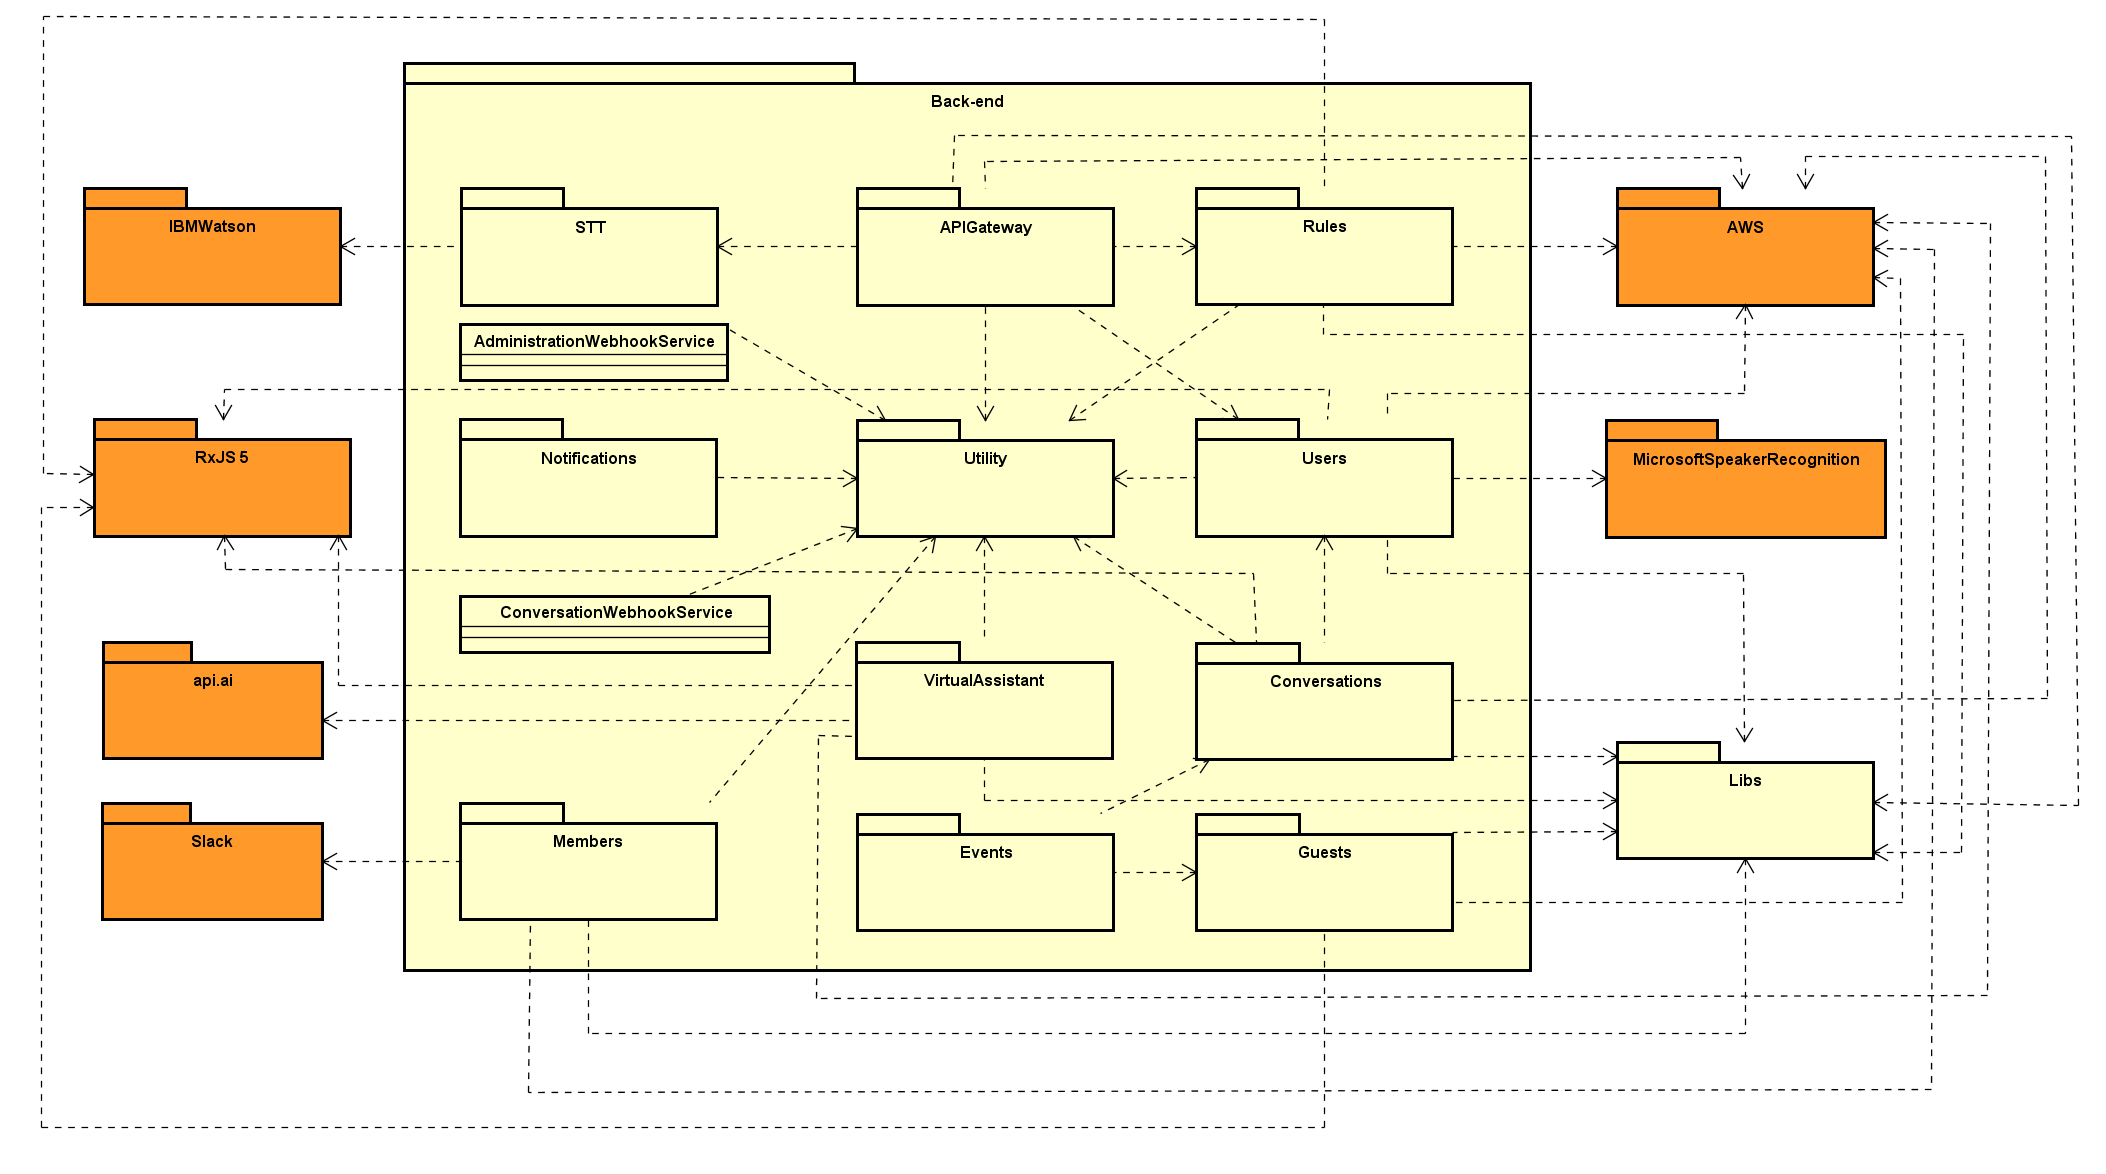
\includegraphics[width=\textwidth,height=\textheight,keepaspectratio]{images/diagrams/back-end/Official_Backend_0304/Back-end.png}
	\caption{Package Back-end}
\end{figure}
\newpage
\paragraph{Classi}
\hypertarget{AdministrationWebhookService_label}{\subparagraph{AdministrationWebhookService}}
\begin{figure}[h]
	\centering
	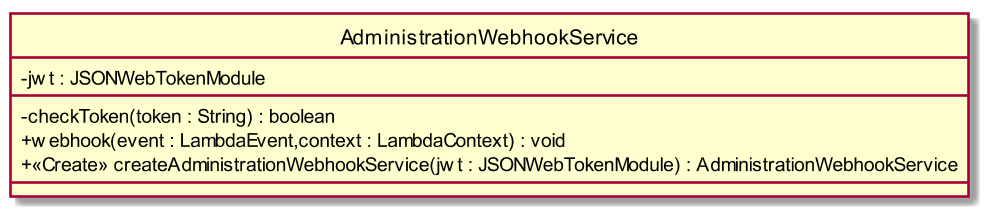
\includegraphics[width=\textwidth,height=\textheight,keepaspectratio]{images/ClassAdministrationWebhookService.png}
	\caption{Back-end::AdministrationWebhookService}
\end{figure}
\begin{itemize}
	\item \textbf{Nome}: \file{AdministrationWebhookService};
	\item \textbf{Tipo}: \file{Class};
	\item \textbf{Descrizione}: questa classe si occupa di implementare l'interfaccia \file{WebhookService}, realizzando un Webhook che fornisce una risposta all'\file{Agent} di amministrazione;
	\item \textbf{Utilizzo}: fornisce il metodo che si occupa di rispondere alle chiamate al \gl{microservizio} da parte dell'\file{Agent} di amministrazione;
	\item \textbf{Padre}: \file{<<interface>> WebhookService};
	\item \textbf{Attributi}:
	\begin{itemize}
		\item[] \file{- jwt: JSONWebTokenModule} \\
		Attributo contenente un riferimento al modulo di \gl{Node.js} per la gestione dei JSON Web Tokens, il quale permette di verificare la validità di un determinato token e di estrarre i dati presenti al suo interno;
	\end{itemize}
	\item \textbf{Metodi}:
	\begin{itemize}
		\item[] \file{- checkToken(token: String): boolean} \\		Metodo che permette di controllare l'autenticità di un JWT. Utilizzato dal metodo \file{webhook} per controllare che la richiesta sia stata fatta da un amministratore autenticato prima di compiere qualsiasi altra azione;\\
		Parametri:
		\begin{itemize}
			\item \file{token: String} \\
			Parametro contenente il JWT per l'autenticazione;
		\end{itemize}
		\item[] \file{+ webhook(event: LambdaEvent, context: LambdaContext): void} \\		Questo metodo soddisfa i requisiti per webhook descritti da api.ai. Viene chiamato ad ogni interazione dell'agente di amministrazione, e si occupa di verificare che nella richiesta sia presente un JSON Web Token (JWT) che confermi un'autenticazione avvenuta con successo. In caso di mancata autenticazione, il campo \file{status} della risposta sarà impostato a 403.  Nel caso in cui il token sia presente e valido (la firma sia valida ed il token non sia scaduto), tale campo sarà invece impostato a 200, ed il campo \file{speech} sarà copiato da \file{fulfillment.speech} della richiesta, risultando quindi in una risposta uguale a quella definita nell'agente di api.ai;\\
		Parametri:
		\begin{itemize}
			\item \file{event: LambdaEvent} \\
			Parametro contenente, all'interno del campo \file{body} sotto forma di stringa in formato JSON, un oggetto con tutti i dati relativi ad una richiesta di api.ai, contenente il token da validare, a \file{AdministrationWebhookService}. Tali dati sono:
			\begin{lstlisting}[language=json,firstnumber=1]
			{
			"id":"String",
			"lang":"String",
			"originalRequest":{
			"source":"String",
			"data":{
			"token":"JWToken"
			}
			}
			"result":"ProcessingResult",
			"sessionId":"String",
			"status":"StatusObject",
			"timestamp":"String"
			}
			\end{lstlisting}
			Per la relativa documentazione, consultare la pagina \url{https://docs.api.ai/docs/query#response} (visitato in data 2017-03-21);
			\item \file{context: LambdaContext} \\
			Parametro utilizzato dal webhook per inviare la risposta. La risposta, contenuta nel \file{LambdaResponse}, parametro del metodo \file{LambdaContext::succeed}, possiede un attributo \file{body}, il quale conterrà il corpo di essa sotto forma di una stringa in formato JSON. \\
			La risposta può essere organizzata in due modi diversi a seconda se il JWT è valido o meno.\\
			Nel caso il JWT sia valido, l'attributo \file{LambdaResponse::statusCode} sarà pari a 200. \\
			Nel caso il JWT non sia valido, l'attributo \file{LambdaResponse::statusCode} sarà pari a 403.
		\end{itemize}
		\item[] \file{+ <<Create>> createAdministrationWebhookService(jwt: JSONWebTokenModule)\\: AdministrationWebhookService} \\		Costruttore che si occupa di effettuare la \gl{dependency injection} di \file{JSONWebTokenModule};\\
		Parametri:
		\begin{itemize}
			\item \file{jwt: JSONWebTokenModule} \\
			Parametro contenente il riferimento al modulo Node.js per la gestione dei JSON Web Tokens;
		\end{itemize}
	\end{itemize}
	\item \textbf{Relazioni con le altre classi}:
	\begin{itemize}
		\item OUT \hyperlink{<<interface>> RulesDAO_label}{\file{<<interface>> RulesDAO}}
		\item OUT \hyperlink{<<interface>> UsersDAO_label}{\file{<<interface>> UsersDAO}}
		\item OUT \hyperlink{LambdaEvent_label}{\file{LambdaEvent}}
	\end{itemize}
\end{itemize}
\FloatBarrier

\hypertarget{ConversationWebhookService_label}{\subparagraph{ConversationWebhookService}}
\begin{figure}[h]
	\centering
	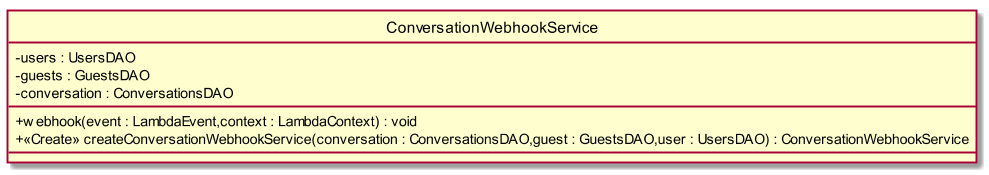
\includegraphics[width=0.80\textwidth,height=\textheight,keepaspectratio]{images/ClassConversationWebhookService.png}
	\caption{Back-end::ConversationWebhookService}
\end{figure}
\begin{itemize}
	\item \textbf{Nome}: \file{ConversationWebhookService};
	\item \textbf{Tipo}: \file{Class};
	\item \textbf{Descrizione}: questa classe si occupa di implementare l'interfaccia \file{WebhookService}, implementando un Webhook che fornisce una risposta ad api.ai;
	\item \textbf{Utilizzo}: fornisce il metodo che si occupa di rispondere alle chiamate fatte al webhook da parte di api.ai;
	\item \textbf{Padre}: \file{<<interface>> WebhookService};
	\item \textbf{Attributi}:
	\begin{itemize}
		\item[] \file{- users: UsersDAO} \\
		Attributo che permette di contattare \file{UsersDAO}, il quale fornisce i meccanismi di accesso al database contenente gli utenti registrati;
		\item[] \file{- guests: GuestsDAO} \\
		Attributo che permette di contattare \file{GuestDAO}, il quale fornisce i meccanismi di accesso al database contenente gli ospiti;
		\item[] \file{- conversation: ConversationsDAO} \\
		Attributo che permette di contattare \file{ConversationDAO}, il quale fornisce i meccanismi di accesso al database delle conversazioni;
	\end{itemize}
	\item \textbf{Metodi}:
	\begin{itemize}
		\item[] \file{+ webhook(event: LambdaEvent, context: LambdaContext): void} \\		Questo metodo soddisfa i requisiti per webhook descritti da api.ai. Si occupa di cercare nei database la presenza di incontri passate con la persona con cui sta avvenendo l'interazione, e di verificare se la persona in questione può essere un amministratore del \gl{sistema}. Nel caso di interazioni passate il \file{context} accoglienza viene riempito con azienda e dati della persona con cui l'ospite ha avuto il maggior numero di incontri in passato, e viene chiesto di confermare se la persona indicata è quella a cui l'ospite è effettivamente interessato. Nel caso di amministratore viene impostato il \file{context} admin, in modo che api.ai riconosca l'utente come un potenziale amministratore e gli chieda se vuole entrare nell'area di amministrazione;\\
		Parametri:
		\begin{itemize}
			\item \file{event: LambdaEvent} \\
			Parametro contenente, all'interno del campo \file{body} sotto forma di stringa in formato JSON, un oggetto con tutti i dati relativi ad una richiesta di api.ai al \\ \file{ConversationWebhookService}. Tali dati sono:
			\begin{lstlisting}[language=json,firstnumber=1]
			{
			"id":"String",
			"lang":"String",
			"originalRequest":"Object",
			"result":"ProcessingResult",
			"sessionId":"String",
			"status":"StatusObject",
			"timestamp":"String"
			}
			\end{lstlisting}
			Per la relativa documentazione, consultare la pagina \url{https://docs.api.ai/docs/query#response} (visitato in data 2017-03-21);
			\item \file{context: LambdaContext} \\
			Parametro utilizzato dal webhook per inviare la risposta. La risposta, contenuta nel \file{LambdaResponse}, parametro del metodo \file{LambdaContext::succeed}, possiede un attributo \file{body}, il quale conterrà il corpo di essa sotto forma di una stringa in formato JSON. \\
			La risposta può essere una tra i seguenti tipi:
			\begin{itemize}
				\item l'utente viene riconosciuto come un potenziale amministratore;
				\item l'utente viene riconosciuto come un ospite conosciuto.
			\end{itemize}
			Nel primo caso, la risposta fornita sarà così organizzata:
			\begin{lstlisting}[language=json,firstnumber=1]
			{
			"contexts": [{
			"context_name":"String",
			"name":"String",
			"username":"String"
			}]
			}
			\end{lstlisting}
			Dove
			\begin{itemize}
				\item \file{context\_name} indica il nome del context, che in questo caso sarà "admin";
				\item \file{name} indica il nome dell'amministratore;
				\item \file{username} indica lo username dell'amministratore;
			\end{itemize}
			Nel secondo caso, la risposta sarà così organizzata:
			\begin{lstlisting}[language=json,firstnumber=1]
			{
			"contexts": [{
			"context_name":"String",
			"guest_name":"String",
			"company":"String",
			"name":"String",
			}]
			}
			\end{lstlisting}
			Dove
			\begin{itemize}
				\item \file{context\_name} indica il nome del context, che in questo caso sarà "welcome";
				\item \file{guest\_name} indica il nome dell'ospite;
				\item \file{company} indica l'azienda di provenienza dell'ospite;
				\item \file{username} indica lo username dell'amministratore;
				\item \file{name} indica il nome della persona desiderata;
			\end{itemize}
		\end{itemize}
		\item[] \file{+ <<Create>> createConversationWebhookService(conversation: ConversationsDAO\\, guest: GuestsDAO, user: UsersDAO): ConversationWebhookService} \\		Metodo che permette la costruzione di un \file{ConversationWebhookService}. Permette la dependency injection che ha come oggetti un \file{ConversationsDAO}, \file{GuestsDAO} e \file{UsersDAO};\\
		Parametri:
		\begin{itemize}
			\item \file{conversation: ConversationsDAO} \\
			Attributo contenente il  \file{ConversationsDAO};
			\item \file{guest: GuestsDAO} \\
			Attributo contenente il \file{GuestsDAO};
			\item \file{user: UsersDAO} \\
			Attributo contenente lo \file{UsersDAO};
		\end{itemize}
	\end{itemize}
	\item \textbf{Relazioni con le altre classi}:
	\begin{itemize}
		\item OUT \hyperlink{LambdaContext_label}{\file{LambdaContext}}
		\item OUT \hyperlink{<<interface>> GuestsDAO_label}{\file{<<interface>> GuestsDAO}}
		\item OUT \hyperlink{<<interface>> UsersDAO_label}{\file{<<interface>> UsersDAO}}
		\item OUT \hyperlink{LambdaEvent_label}{\file{LambdaEvent}}
		\item OUT \hyperlink{<<interface>> ConversationsDAO_label}{\file{<<interface>> ConversationsDAO}}
	\end{itemize}
\end{itemize}
\FloatBarrier

\hypertarget{SNSEvent_label}{\subparagraph{SNSEvent}}
\begin{figure}[h]
	\centering
	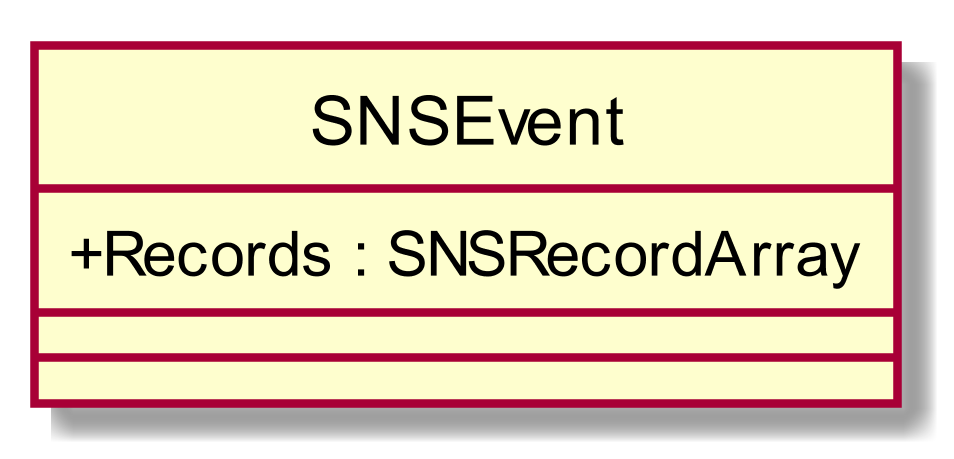
\includegraphics[width=0.35\textwidth,height=\textheight,keepaspectratio]{images/ClassSNSEvent.png}
	\caption{Back-end::SNSEvent}
\end{figure}
\begin{itemize}
	\item \textbf{Nome}: \file{SNSEvent};
	\item \textbf{Tipo}: \file{Class};
	\item \textbf{Descrizione}: questa classe rappresenta l'oggetto ricevuto da una Lambda Function in seguito alla pubblicazione di un messaggio su un topic di SNS a cui tale funzione è iscritta;
	\item \textbf{Utilizzo}: fornisce gli attributi relativi ad una notifica mandata da SNS ad una Lambda Function iscritta ad un topic sul quale sia stato pubblicato un messaggio;
	\item \textbf{Attributi}:
	\begin{itemize}
		\item[] \file{+ Records: SNSRecordArray} \\
		Array contenente i dati della notifica mandata da SNS alla Lambda Function. Contiene un unico oggetto di tipo Record;
	\end{itemize}
	\item \textbf{Relazioni con le altre classi}:
	\begin{itemize}
		\item IN \hyperlink{VAMessageListener_label}{\file{VAMessageListener}}
		\item OUT \hyperlink{SNSRecord_label}{\file{SNSRecord}}
	\end{itemize}
\end{itemize}
\FloatBarrier


\newpage \subsubsection{Back-end::APIGateway}
Package contenente le classi necessarie a gestire:
\begin{itemize}
	\item diversi tipi di  dispositivi client;
	\item l'interazione tra \file{Client} e \file{Back-end};
	\item la combinazione tra i servizi supportati dal \file{Back-end}.
\end{itemize}
\begin{figure}[h] \centering 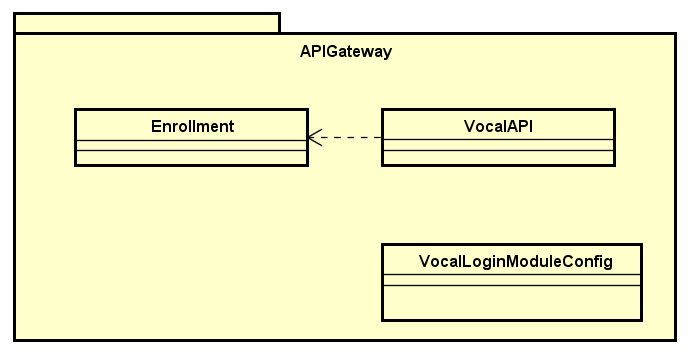
\includegraphics[width=\textwidth,height=\textheight,keepaspectratio]{images/diagrams/back-end/Official_Backend_0304/APIGateway.png}
	\caption{Package Back-end::APIGateway}
\end{figure}
\newpage

\paragraph{Classi}
\hypertarget{Enrollment_label}{\subparagraph{Enrollment}}
\begin{figure}[h]
	\centering
	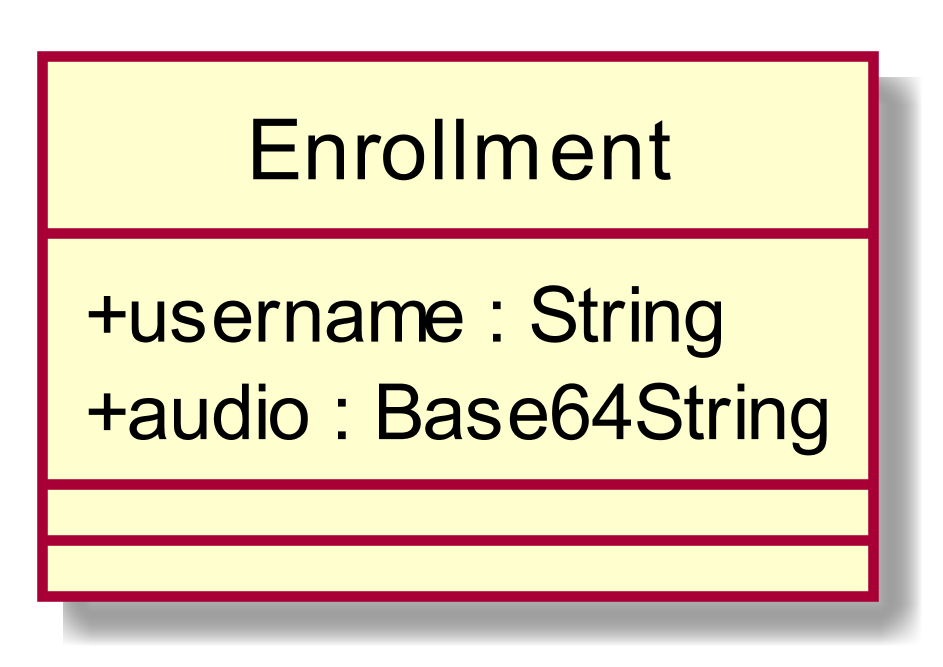
\includegraphics[width=0.35\textwidth,height=\textheight,keepaspectratio]{images/ClassEnrollment.png}
	\caption{Back-end::APIGateway::Enrollment}
\end{figure}
\begin{itemize}
	\item \textbf{Nome}: \file{Enrollment};
	\item \textbf{Tipo}: \file{Class};
	\item \textbf{Descrizione}: questa classe fornisce gli attributi necessari al passaggio di un \file{Enrollment} alle Lambda Function;
	\item \textbf{Utilizzo}: fornisce gli attributi relativi ad un \file{Enrollment};
	\item \textbf{Attributi}:
	\begin{itemize}
		\item[] \file{+ username: String} \\
		Attributo contenente l'username dell'utente associato all'\file{Enrollment};
		\item[] \file{+ audio: Base64String} \\
		Attributo contenente la traccia audio che sarà oggetto dell'\file{Enrollment}, codificata in Base64;
	\end{itemize}
	\item \textbf{Relazioni con le altre classi}:
	\begin{itemize}
		\item IN \hyperlink{VocalAPI_label}{\file{VocalAPI}}
	\end{itemize}
\end{itemize}
\FloatBarrier

\hypertarget{VocalAPI_label}{\subparagraph{VocalAPI}}
\begin{figure}[h]
	\centering
	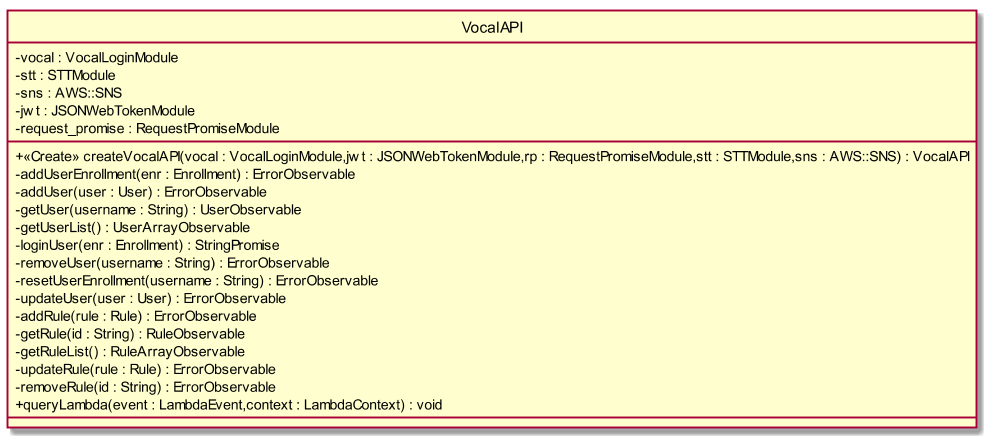
\includegraphics[width=\textwidth,height=\textheight,keepaspectratio]{images/ClassVocalAPI.png}
	\caption{Back-end::APIGateway::VocalAPI}
\end{figure}
\begin{itemize}
	\item \textbf{Nome}: \file{VocalAPI};
	\item \textbf{Tipo}: \file{Class};
	\item \textbf{Descrizione}: questa classe si occupa di implementare l'\gl{endpoint} dell'\gl{API Gateway} utilizzato dal client vocale;
	\item \textbf{Utilizzo}: fornisce un metodo pubblico che si occupa di implementare l'handler per la Lambda Function collegata all'endpoint utilizzato dal client. Definisce inoltre una serie di metodi privati che si occupano di portare a termine le diverse azioni che vengono richieste dall'assistente virtuale;
	\item \textbf{Attributi}:
	\begin{itemize}
		\item[] \file{- vocal: VocalLoginModule} \\
		Attributo contenente il \file{VocalLoginModule} di cui è stata eseguita la dependency injection nel costruttore. Viene utilizzato per effettuare il login nel servizio di Speaker Recognition;
		\item[] \file{- stt: STTModule} \\
		Attributo contenente il modulo utilizzato per contattare le API per il servizio di Watson Speech to Text di IBM;
		\item[] \file{- sns: AWS::SNS} \\
		Attributo che permette di contattare il servizio SNS;
		\item[] \file{- jwt: JSONWebTokenModule} \\
		Attributo contenente il \file{JSONWebTokenModule} di cui è stata eseguita la dependency injection nel costruttore. Viene utilizzato per creare un JSONWebToken in caso di autenticazione al sistema avvenuta con successo;
		\item[] \file{- request\_promise: RequestPromiseModule} \\
		Attributo contenente il \file{RequestPromiseModule} di cui è stata eseguita la dependency injection nel costruttore. Viene utilizzato per effettuare richieste \gl{HTTP} sostituendo \gl{callback}s con promises;
	\end{itemize}
	\item \textbf{Metodi}:
	\begin{itemize}
		\item[] \file{+ <<Create>> createVocalAPI(vocal: VocalLoginModule, jwt: JSONWebTokenModule\\, rp: RequestPromiseModule, stt: STTModule, sns: AWS::SNS): VocalAPI} \\		Costruttore della classe \file{VocalAPI} che permette la dependency injection dei moduli richiesti;\\
		Parametri:
		\begin{itemize}
			\item \file{vocal: VocalLoginModule} \\
			Parametro che permette di effettuare la dependency injection di \file{VocalLoginModule};
			\item \file{jwt: JSONWebTokenModule} \\
			Parametro che permette di effettuare la dependency injection di \file{JSONWebTokenModule};
			\item \file{rp: RequestPromiseModule} \\
			Parametro che permette di effettuare la dependency injection di \file{RequestPromiseModule};
			\item \file{stt: STTModule} \\
			Parametro contenente l'\file{STTModule} di cui si vuole fare la dependency injection;
			\item \file{sns: AWS::SNS} \\
			Parametro contenente il modulo \file{AWS::SNS} del quale si vuole effettuare la dependency injection;
		\end{itemize}
		\item[] \file{- addUserEnrollment(enr: Enrollment): ErrorObservable} \\		Metodo che permette di aggiungere un \gl{enrollment} ad un utente del sistema. Restituisce un oggetto di tipo \file{ErrorObservable} e, in caso di errore, notifica l'\file{Error\gl{Observer}} chiamando il suo metodo \file{error} utilizzando come parametro un oggetto \file{Exception} con code impostato a 1 nel caso in cui l'utente non esista. In assenza di errori, viene chiamato il metodo il metodo \file{complete};\\
		Parametri:
		\begin{itemize}
			\item \file{enr: Enrollment} \\
			Parametro contenente l'enrollment da aggiungere a un utente;
		\end{itemize}
		\item[] \file{- addUser(user: User): ErrorObservable} \\		Metodo che permette di aggiungere un utente al sistema. Restituisce un oggetto di tipo \file{ErrorObservable} e, in caso di errore, notifica l'\file{ErrorObserver} chiamando il suo metodo \file{error} utilizzando come parametro un oggetto \file{Exception} con code impostato a 1 in caso di username già esistente, 2 in caso di username non valido (troppo lungo o troppo corto). In assenza di errori, viene chiamato il metodo il metodo \file{complete};\\
		Parametri:
		\begin{itemize}
			\item \file{user: User} \\
			Parametro contenente l'user che si vuole aggiungere al sistema;
		\end{itemize}
		\item[] \file{- getUser(username: String): UserObservable} \\		Metodo che permette di ottenere i dati relativi ad un utente del sistema. Restituisce l'oggetto \file{User} relativo all'utente con lo username indicato. In caso tale utente non esista, restituisce un oggetto vuoto;\\
		Parametri:
		\begin{itemize}
			\item \file{username: String} \\
			Parametro contente l'username dell'utente del quale si vogliono ottenere i dati;
		\end{itemize}
		\item[] \file{- getUserList(): UserArrayObservable} \\		Metodo che permette di ottenere una lista degli utenti del sistema;\\
		\item[] \file{- loginUser(enr: Enrollment): StringPromise} \\		Metodo che si occupa di gestire il login vocale degli utenti. Restituisce una stringa contenente il JWT in caso di autenticazione avvenuta con successo, altrimenti restituisce una stringa vuota;\\
		Parametri:
		\begin{itemize}
			\item \file{enr: Enrollment} \\
			Attributo contenente l'\file{Enrollment} (\file{audio} + \file{username}) con il quale tentare il login;
		\end{itemize}
		\item[] \file{- removeUser(username: String): ErrorObservable} \\		Metodo che permette di eliminare i dati relativi ad un utente dal sistema. Restituisce un oggetto di tipo \file{ErrorObservable} e, in caso di errore, notifica l'\file{ErrorObserver} chiamando il suo metodo \file{error} utilizzando come parametro un oggetto \file{Exception} con code impostato a 1 nel caso in cui l'utente non esista. In assenza di errori, viene chiamato il metodo il metodo \file{complete};\\
		Parametri:
		\begin{itemize}
			\item \file{username: String} \\
			Parametro contenente l'username dell'user da eliminare dal sistema;
		\end{itemize}
		\item[] \file{- resetUserEnrollment(username: String): ErrorObservable} \\		Metodo che permette di eliminare tutti gli enrollments di un utente del sistema. Restituisce un oggetto di tipo \file{ErrorObservable} e, in caso di errore, notifica l'\file{ErrorObserver} chiamando il suo metodo \file{error} utilizzando come parametro un oggetto \file{Exception} con code impostato a 1 nel caso in cui l'utente non esista. In assenza di errori, viene chiamato il metodo il metodo \file{complete};\\
		Parametri:
		\begin{itemize}
			\item \file{username: String} \\
			Parametro contenente l'username dell utente a cui si vogliono eliminare tutti gli enrollments;
		\end{itemize}
		\item[] \file{- updateUser(user: User): ErrorObservable} \\		Metodo che permette di modificare i dati relativi ad un utente del sistema. Restituisce un oggetto di tipo \file{ErrorObservable} e, in caso di errore, notifica l'\file{ErrorObserver} chiamando il suo metodo \file{error} utilizzando come parametro un oggetto \file{Exception} con code impostato a 1 nel caso in cui l'utente non esista. In assenza di errori, viene chiamato il metodo il metodo \file{complete};\\
		Parametri:
		\begin{itemize}
			\item \file{user: User} \\
			Parametro contenente l'\file{User} da modificare;
		\end{itemize}
		\item[] \file{- addRule(rule: Rule): ErrorObservable} \\		Metodo che permette di aggiungere una \gl{direttiva} al sistema. Restituisce un oggetto di tipo \file{ErrorObservable};\\
		Parametri:
		\begin{itemize}
			\item \file{rule: Rule} \\
			Parametro contenente la \file{Rule};
		\end{itemize}
		\item[] \file{- getRule(id: String): RuleObservable} \\		Metodo che permette di ottenere i dati relativi ad una direttiva del sistema a partire dal suo id. Restituisce la direttiva in questione, oppure un oggetto vuoto nel caso in cui tale direttiva non esista;\\
		Parametri:
		\begin{itemize}
			\item \file{id: String} \\
			Parametro contenente l'identificativo della \file{Rule};
		\end{itemize}
		\item[] \file{- getRuleList(): RuleArrayObservable} \\		Metodo che permette di ottenere la lista delle \gl{direttive} del sistema.
		;\\
		\item[] \file{- updateRule(rule: Rule): ErrorObservable} \\		Metodo che permette di aggiornare una direttiva presente nel sistema. Restituisce un oggetto di tipo \file{ErrorObservable};\\
		Parametri:
		\begin{itemize}
			\item \file{rule: Rule} \\
			Parametro contenente la \file{Rule} aggiornata;
		\end{itemize}
		\item[] \file{- removeRule(id: String): ErrorObservable} \\		Metodo che permette di rimuovere una direttiva presente nel sistema. Restituisce un oggetto di tipo \file{ErrorObservable};\\
		Parametri:
		\begin{itemize}
			\item \file{id: String} \\
			Parametro contenente l'identificativo della \file{Rule};
		\end{itemize}
		\item[] \file{+ queryLambda(event: LambdaEvent, context: LambdaContext): void} \\\\		Metodo che si occupa di chiamare prima il servizio di Speech To Text e, una volta ottenuta risposta da esso, di interrogare l'assistente virtuale. Quando viene ricevuta una risposta dall'assistente virtuale, il metodo controlla il valore del campo \file{action} di tale risposta e, nel caso in cui corrisponda ad una delle action supportate, si occupa di eseguire le azioni necessarie utilizzando i metodi privati di questa classe. Nel caso in cui invece \file{action} non corrisponda ad una delle azioni supportate (ovvero action è un'azione che non richiede operazione da parte del back-end, oppure \file{actionIncomplete} è impostato a true), tale risposta viene rielaborata ed inoltrata. Le azioni supportate ed i relativi compiti da svolgere sono disponibili alla sezione \ref{action}. \\
		Ad ogni interazione viene inoltre pubblicato un messaggio su un topic di sns, utilizzando il metodo \file{sns.publish}, in modo che sia possibile registrare i dati relativi a tali interazioni e mandare le notifiche ai membri interessati;\\
		Parametri:
		\begin{itemize}
			\item \file{event: LambdaEvent} \\
			Parametro contenente, all'interno del campo \file{body} sotto forma di stringa in formato JSON, un oggetto contenente tutti i dati relativi ad un messaggio ricevuto da API Gateway. Tali dati saranno nel seguent formato:
			\begin{lstlisting}[language=json,firstnumber=1]
			{
			"app":"String",
			"audio": "Base64String",
			"data": "ObjectAssocArray",
			"sesssion_id":"String"
			}
			\end{lstlisting}
			
			Nel caso in cui il campo \file{audio} risulti vuoto, il metodo andrà a cercare l'attributo \file{data.speech} e lo utilizzerà come stringa per interrogare l'assistente virtuale, senza passare per il microservizio di Speech To Text. Questo permette di fornire input testuale e non vocale all'assistente virtuale nei casi in cui sia necessario, ad esempio dopo un certo numero di tentativi di comunicare delle informazioni senza successo;
			\item \file{context: LambdaContext} \\
			Parametro utilizzato dalle Lambda Function per inviare la risposta. La risposta, contenuta nel \file{LambdaResponse} parametro del metodo \file{LambdaContext::succeed}, possiede un attributo \file{body}, il quale conterrà il corpo di essa sotto forma di una stringa in formato JSON, organizzando i dati nel seguente modo:
			\begin{lstlisting}[language=json,firstnumber=1]
			{
			"action":"String",
			"res":{
			"contexts":"ObjectAssocArray",
			"data":"Object",
			"text_request":"String",
			"text_response":"String"
			},
			"sesssion_id":"String"
			}
			\end{lstlisting};
		\end{itemize}
	\end{itemize}
	\item \textbf{Relazioni con le altre classi}:
	\begin{itemize}
		\item OUT \hyperlink{Enrollment_label}{\file{Enrollment}}
		\item OUT \hyperlink{Rule_label}{\file{Rule}}
		\item OUT \hyperlink{<<interface>> STTModule_label}{\file{<<interface>> STTModule}}
		\item OUT \hyperlink{<<interface>>VocalLoginModule_label}{\file{<<interface>>VocalLoginModule}}
		\item OUT \hyperlink{User_label}{\file{User}}
		\item OUT \hyperlink{LambdaContext_label}{\file{LambdaContext}}
		\item OUT \hyperlink{LambdaEvent_label}{\file{LambdaEvent}}
		\item OUT \hyperlink{VARequestAPIBody_label}{\file{VARequestAPIBody}}
	\end{itemize}
\end{itemize}
\FloatBarrier

\hypertarget{VocalLoginModuleConfig_label}{\subparagraph{VocalLoginModuleConfig}}
\begin{figure}[h]
	\centering
	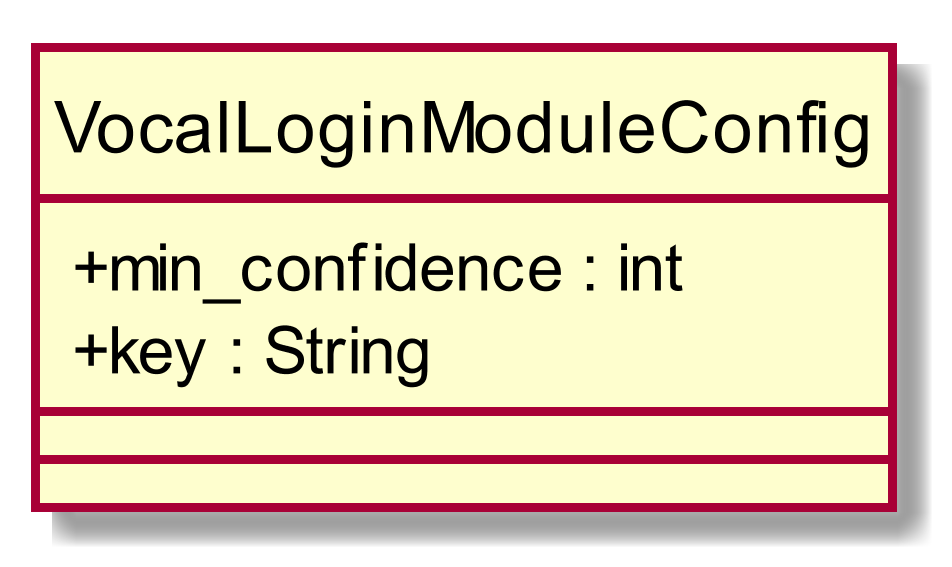
\includegraphics[width=0.35\textwidth,height=\textheight,keepaspectratio]{images/ClassVocalLoginModuleConfig.png}
	\caption{Back-end::APIGateway::VocalLoginModuleConfig}
\end{figure}
\begin{itemize}
	\item \textbf{Nome}: \file{VocalLoginModuleConfig};
	\item \textbf{Tipo}: \file{Class};
	\item \textbf{Descrizione}: questa classe viene utilizzata per la configurazione di \file{VocalLoginModule};
	\item \textbf{Utilizzo}: fornisce gli attributi necessari alla configurazione di \file{VocalLoginModule};
	\item \textbf{Attributi}:
	\begin{itemize}
		\item[] \file{+ min\_confidence: int} \\
		Questo attributo indica la confidence minima richiesta perchè il login avvenga con successo;
		\item[] \file{+ key: String} \\
		Chiave di accesso alle API del vocal login module;
	\end{itemize}
	\item \textbf{Relazioni con le altre classi}:
	\begin{itemize}
		\item IN \hyperlink{VocalLoginMicrosoftModule_label}{\file{VocalLoginMicrosoftModule}}
	\end{itemize}
\end{itemize}
\FloatBarrier

\newpage \subsubsection{Back-end::Conversations}
Package contenente le classi relative alle Conversations del sistema.
\begin{figure}[h] \centering 
	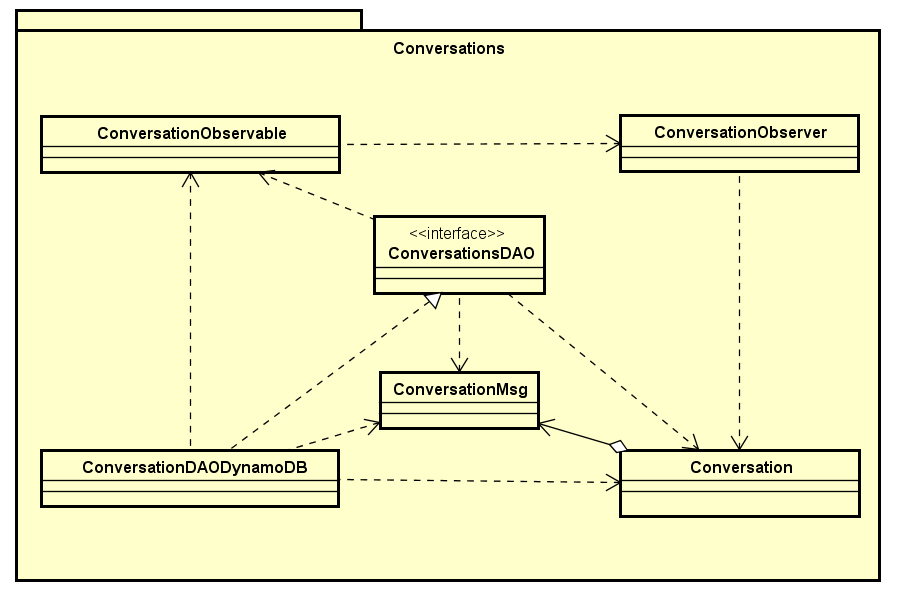
\includegraphics[width=\textwidth,height=\textheight,keepaspectratio]{images/diagrams/back-end/Official_Backend_0304/Conversations.png}
	\caption{Package Back-end::Conversations}
\end{figure}
\newpage

\paragraph{Classi}
\hypertarget{ ConversationsDAO_label}{\subparagraph{ ConversationsDAO}}
\begin{figure}[h]
	\centering
	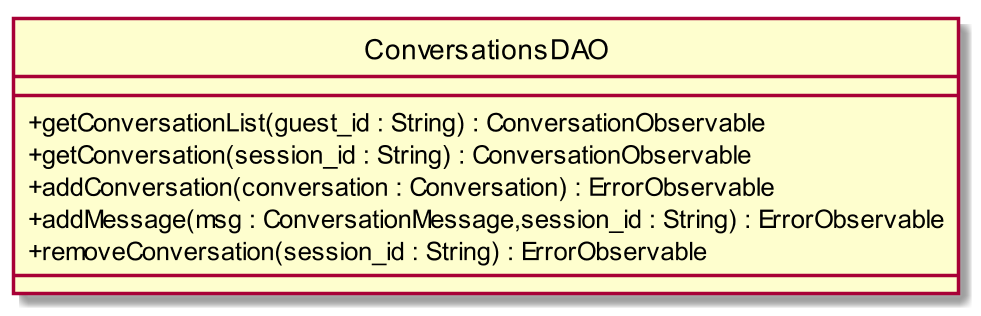
\includegraphics[width=0.60\textwidth,height=\textheight,keepaspectratio]{images/ClassConversationsDAO.png}
	\caption{Back-end::Conversations:: ConversationsDAO}
\end{figure}
\begin{itemize}
	\item \textbf{Nome}: \file{ ConversationsDAO};
	\item \textbf{Tipo}: \file{Interface};
	\item \textbf{Descrizione}: questa classe si occupa di astrarre le modalità d'interazione con il database contenente le conversazioni;
	\item \textbf{Utilizzo}: fornisce a \file{ConversationWebhookService} un meccanismo per accedere al database contenente le conversazioni, senza conoscerne le modalità di implementazioni e di persistenza di quest'ultimo. Permette operazioni di lettura, scrittura e rimozione di conversazioni;
	\item \textbf{Figlio}: \file{ConversationsDAODynamoDB};
	\item \textbf{Metodi}:
	\begin{itemize}
		\item[] \file{+ getConversationList(guest\_id: String): ConversationObservable}\\ \\		Metodo che permette di ottenere una conversazione a partire dall'identificativo di un \file{Guest}. L'\file{Observable} restituito manderà agli \file{Observer} le conversazioni ottenute, una alla volta, e poi chiama il loro metodo \file{complete}. Nel caso in cui si verifichi un errore, l'\file{Observer} iscritto verrà notificato tramite la chiamata del suo metodo \file{error} con i dati relativi all'errore verificatosi;\\
		Parametri:
		\begin{itemize}
			\item \file{guest\_id: String} \\
			Stringa identificativa dell'ospite del quale si vogliono ottenere le conversazioni. Nel caso in cui venga passata una stringa vuota, il metodo deve restituire un array contenente tutte le conversazioni avvenute con tutti gli ospiti;
		\end{itemize}
		\item[] \file{+ getConversation(session\_id: String): ConversationObservable} \\\\		Metodo che permette di ottenere una conversazione a partire dall'identificativo della sessione. L'\file{Observable} restituito riceverà l'oggetto rappresentante tale \file{Conversation}, e verrà completato. Nel caso in cui la conversazione richiesta non sia presente nel database, gli \file{Observer} interessati non riceveranno alcun valore, ma verranno notificati tramite la chiamata del loro metodo \file{error};\\
		Parametri:
		\begin{itemize}
			\item \file{session\_id: String} \\
			Parametro contenente l'id della sessione della conversazione da ricevere;
		\end{itemize}
		\item[] \file{+ addConversation(conversation: Conversation): ErrorObservable} \\\\		Metodo che permette di aggiungere una conversazione. L'\file{Observable} restituito non riceverà alcun valore, ma verrà completato in caso di aggiunta della conversazione avvenuta con successo. In caso di errore durante l'aggiunta della conversazione, gli \file{Observer} interessati verranno notificati tramite la chiamata del loro metodo \file{error} con i dati relativi all'errore verificatosi;\\
		Parametri:
		\begin{itemize}
			\item \file{conversation: Conversation} \\
			Parametro contente la conversazione da inserire;
		\end{itemize}
		\item[] \file{+ addMessage(msg: ConversationMessage, session\_id: String): ErrorObservable}\\ \\		Metodo che permette di aggiungere un messaggio a una conversazione a partire dal messaggio stesso e l'identificativo della conversazione. L'\file{Observable} restituito non riceverà alcun valore, ma verrà completato in caso di aggiunta del messaggio avvenuta con successo. In caso di errore durante l'aggiunta del messaggio, gli \file{Observer} interessati verranno notificati tramite la chiamata del loro metodo \file{error} con i dati relativi all'errore verificatosi;\\
		Parametri:
		\begin{itemize}
			\item \file{msg: ConversationMessage} \\
			Parametro contenente il messaggio;
			\item \file{session\_id: String} \\
			Parametro contenente l'id della sessione della conversazione alla quale aggiungere il messaggio;
		\end{itemize}
		\item[] \file{+ removeConversation(session\_id: String): ErrorObservable} \\		Metodo che permette di rimuovere una conversazione a partire dall'identificativo della sessione. L'\file{Observable} restituito non riceverà alcun valore, ma verrà completato in caso di aggiunta della conversazione avvenuta con successo. In caso di errore durante l'aggiunta della conversazione, gli \file{Observer} interessati verranno notificati tramite la chiamata del loro metodo \file{error} con i dati relativi all'errore verificatosi;\\
		Parametri:
		\begin{itemize}
			\item \file{session\_id: String} \\
			Parametro contenente l'id della sessione della conversazione da eliminare;
		\end{itemize}
	\end{itemize}
	\item \textbf{Relazioni con le altre classi}:
	\begin{itemize}
		\item IN \hyperlink{ConversationWebhookService_label}{\file{ConversationWebhookService}}
		\item IN \hyperlink{VAMessageListener_label}{\file{VAMessageListener}}
		\item OUT \hyperlink{ConversationMsg_label}{\file{ConversationMsg}}
		\item OUT \hyperlink{ConversationObservable_label}{\file{ConversationObservable}}
		\item OUT \hyperlink{Conversation_label}{\file{Conversation}}
		\item OUT \hyperlink{ErrorObservable_label}{\file{ErrorObservable}}
	\end{itemize}
\end{itemize}
\FloatBarrier

\hypertarget{Conversation_label}{\subparagraph{Conversation}}
\begin{figure}[h]
	\centering
	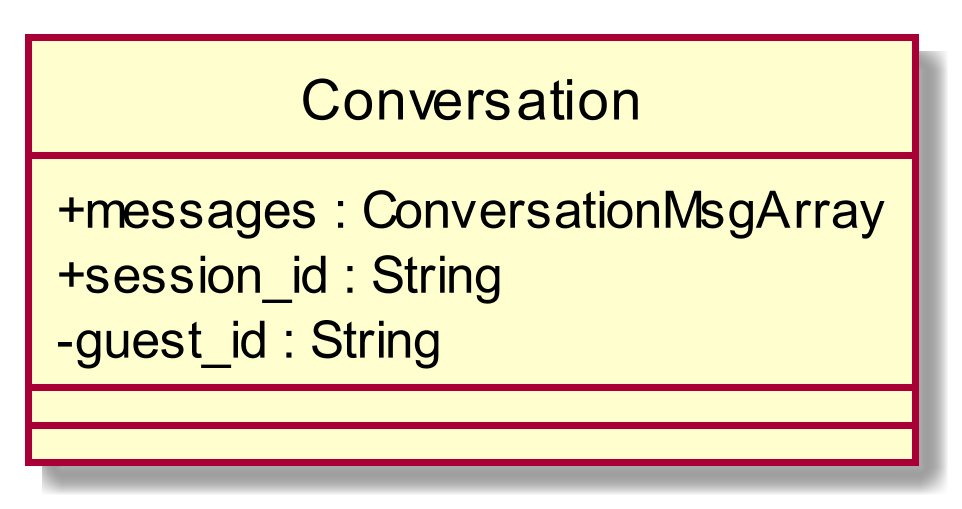
\includegraphics[width=0.35\textwidth,height=\textheight,keepaspectratio]{images/ClassConversation.png}
	\caption{Back-end::Conversations::Conversation}
\end{figure}
\begin{itemize}
	\item \textbf{Nome}: \file{Conversation};
	\item \textbf{Tipo}: \file{Class};
	\item \textbf{Descrizione}: questa classe si occupa di rappresentare e organizzare gli attributi relativi ad una conversazione, la quale dovrà essere salvata nel database;
	\item \textbf{Utilizzo}: fornisce gli attributi relativi ad una conversazione;
	\item \textbf{Attributi}:
	\begin{itemize}
		\item[] \file{+ messages: ConversationMsgArray} \\
		Attributo contenente l'array dei messaggi contenuti in una conversazione;
		\item[] \file{+ session\_id: String} \\
		Attributo contenente l'id della sessione relativa alla conversazione;
		\item[] \file{- guest\_id: String} \\
		Attributo contenente l'identificativo dell'ospite con il quale è avvenuta la conversazione;
	\end{itemize}
	\item \textbf{Relazioni con le altre classi}:
	\begin{itemize}
		\item IN \hyperlink{<<interface>> ConversationsDAO_label}{\file{<<interface>> ConversationsDAO}}
		\item IN \hyperlink{ConversationObserver_label}{\file{ConversationObserver}}
		\item IN \hyperlink{ConversationsDAODynamoDB_label}{\file{ConversationsDAODynamoDB}}
		\item OUT \hyperlink{ConversationMsg_label}{\file{ConversationMsg}}
	\end{itemize}
\end{itemize}
\FloatBarrier

\hypertarget{ConversationMsg_label}{\subparagraph{ConversationMsg}}
\begin{figure}[h]
	\centering
	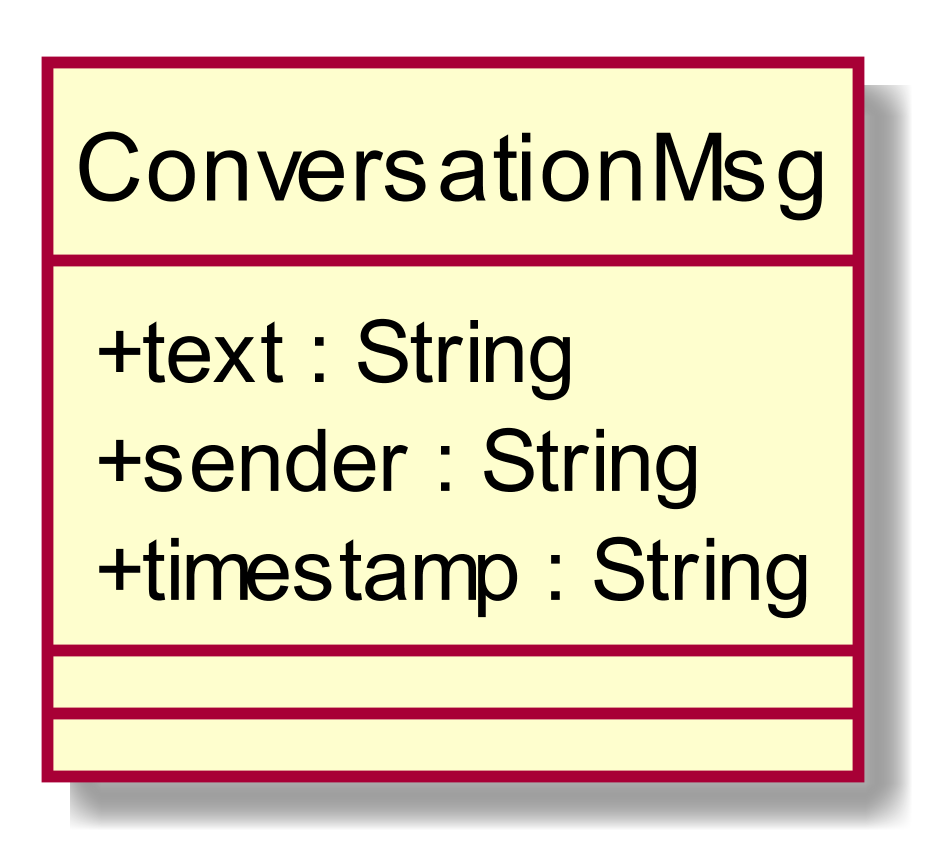
\includegraphics[width=0.35\textwidth,height=\textheight,keepaspectratio]{images/ClassConversationMsg.png}
	\caption{Back-end::Conversations::ConversationMsg}
\end{figure}
\begin{itemize}
	\item \textbf{Nome}: \file{ConversationMsg};
	\item \textbf{Tipo}: \file{Class};
	\item \textbf{Descrizione}: questa classe si occupa di rappresentare e organizzare gli attributi relativi ad un messaggio all'interno di una conversazione;
	\item \textbf{Utilizzo}: fornisce gli attributi relativi un messaggio. La classe \file{Conversation} contiene un array di essi, in modo da costruire l'intera conversazione;
	\item \textbf{Attributi}:
	\begin{itemize}
		\item[] \file{+ text: String} \\
		Attributo contenente il testo del messaggio;
		\item[] \file{+ sender: String} \\
		Attributo contenente il mittente del messaggio;
		\item[] \file{+ timestamp: String} \\
		Attributo contenente il timestamp del messaggio;
	\end{itemize}
	\item \textbf{Relazioni con le altre classi}:
	\begin{itemize}
		\item IN \hyperlink{Conversation_label}{\file{Conversation}}
		\item IN \hyperlink{<<interface>> ConversationsDAO_label}{\file{<<interface>> ConversationsDAO}}
		\item IN \hyperlink{ConversationsDAODynamoDB_label}{\file{ConversationsDAODynamoDB}}
	\end{itemize}
\end{itemize}
\FloatBarrier

\hypertarget{ConversationObservable_label}{\subparagraph{ConversationObservable}}
\begin{figure}[h]
	\centering
	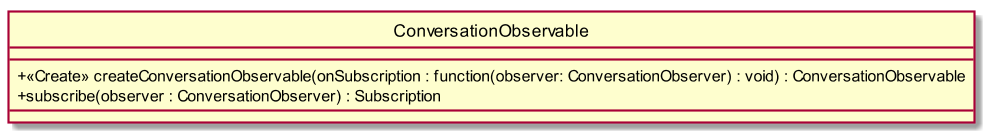
\includegraphics[width=\textwidth,height=\textheight,keepaspectratio]{images/ClassConversationObservable.png}
	\caption{Back-end::Conversations::ConversationObservable}
\end{figure}
\begin{itemize}
	\item \textbf{Nome}: \file{ConversationObservable};
	\item \textbf{Tipo}: \file{Class};
	\item \textbf{Descrizione}: questa classe implementa un \file{Observable} che permette l'iscrizione di \\ \file{ConversationObserver};
	\item \textbf{Utilizzo}: fornisce i meccanismi necessari per il passaggio di una serie di \file{Conversation} ad un \file{Observer} interessato;
	\item \textbf{Padre}: \file{Observable};
	\item \textbf{Metodi}:
	\begin{itemize}
		\item[] \file{+ <<Create>> createConversationObservable(onSubscription: function\\(observer: ConversationObserver) : void): ConversationObservable} \\		Constructor di \file{ConversationObservable};\\
		Parametri:
		\begin{itemize}
			\item \file{onSubscription: function(observer: ConversationObserver) : void} \\
			Funzione che verrà eseguita quando un \file{Observer} si iscrive all'\file{Observable}. Si occupa di passare i dati all'\file{Observer}, chiamando il metodo \file{next(conversation: Conversation)}. Quando non ci sono più dati da restituire, si occupa di chiamare il metodo \file{complete}. Nel caso in cui si verificasse un errore, si occupa di chiamare il metodo \file{error(err: Object)} con i dati relativi all'errore verificatosi;
		\end{itemize}
		\item[] \file{+ subscribe(observer: ConversationObserver): Subscription} \\		Metodo che permette ad uno \file{ConversationObserver} interessato di iscriversi a questo \file{Observable};\\
		Parametri:
		\begin{itemize}
			\item \file{observer: ConversationObserver} \\
			\file{Observer} che si vuole iscrivere;
		\end{itemize}
	\end{itemize}
	\item \textbf{Relazioni con le altre classi}:
	\begin{itemize}
		\item IN \hyperlink{<<interface>> ConversationsDAO_label}{\file{<<interface>> ConversationsDAO}}
		\item IN \hyperlink{ConversationsDAODynamoDB_label}{\file{ConversationsDAODynamoDB}}
		\item OUT \hyperlink{ConversationObserver_label}{\file{ConversationObserver}}
	\end{itemize}
\end{itemize}
\FloatBarrier

\hypertarget{ConversationObserver_label}{\subparagraph{ConversationObserver}}
\begin{figure}[h]
	\centering
	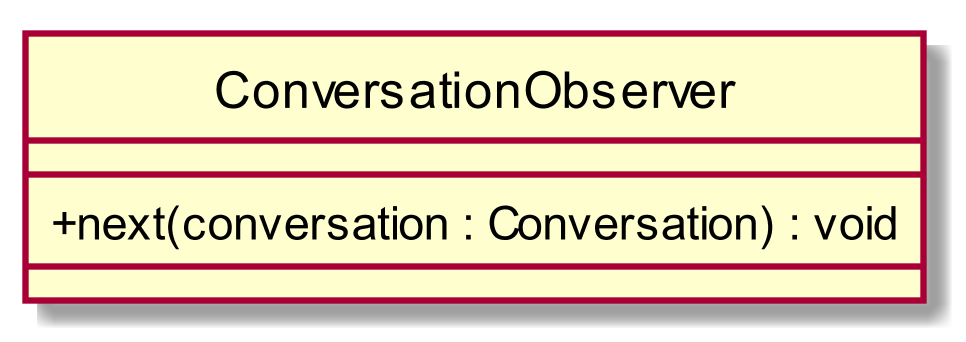
\includegraphics[width=0.35\textwidth,height=\textheight,keepaspectratio]{images/ClassConversationObserver.png}
	\caption{Back-end::Conversations::ConversationObserver}
\end{figure}
\begin{itemize}
	\item \textbf{Nome}: \file{ConversationObserver};
	\item \textbf{Tipo}: \file{Class};
	\item \textbf{Descrizione}: classe che rappresenta un \file{Observer} che si aspetta dati di tipo \file{Conversation};
	\item \textbf{Utilizzo}: ridefinisce il metodo \file{next} della classe \file{ObserverAdapter}, in maniera tale che accetti dati di tipo \file{Conversation};
	\item \textbf{Metodi}:
	\begin{itemize}
		\item[] \file{+ next(conversation: Conversation): void} \\		Metodo che permette agli \file{Observable} di notificare l'\file{Observer} con dati di tipo \file{Conversation}. Definisce inoltre le operazioni che l'\file{Observer} compierà all'arrivo di tali dati;\\
		Parametri:
		\begin{itemize}
			\item \file{conversation: Conversation} \\
			Parametro contenente la \file{Conversation} mandata dall'\file{Observable};
		\end{itemize}
	\end{itemize}
	\item \textbf{Relazioni con le altre classi}:
	\begin{itemize}
		\item IN \hyperlink{ConversationObservable_label}{\file{ConversationObservable}}
		\item OUT \hyperlink{Conversation_label}{\file{Conversation}}
	\end{itemize}
\end{itemize}
\FloatBarrier

\hypertarget{ConversationsDAODynamoDB_label}{\subparagraph{ConversationsDAODynamoDB}}
\begin{figure}[h]
	\centering
	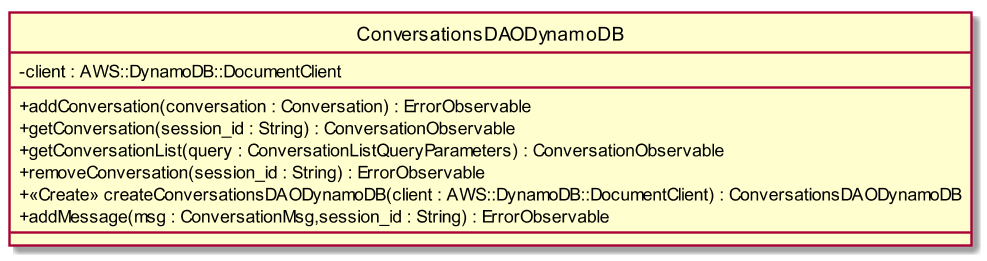
\includegraphics[width=\textwidth,height=\textheight,keepaspectratio]{images/ClassConversationsDAODynamoDB.png}
	\caption{Back-end::Conversations::ConversationsDAODynamoDB}
\end{figure}
\begin{itemize}
	\item \textbf{Nome}: \file{ConversationsDAODynamoDB};
	\item \textbf{Tipo}: \file{Class};
	\item \textbf{Descrizione}: classe che si occupa di implementare l'interfaccia \file{ConversationsDAO}, utilizzando un database DynamoDB come supporto per la memorizzazione dei dati;
	\item \textbf{Utilizzo}: implementa i metodi dell'interfaccia \file{ConversationsDAO} interrogando un database DynamoDB. Utilizza \file{AWS::DynamoDB::DocumentClient} per l'accesso al database. La dependency injection dell'oggetto \file{AWS::DynamoDB} viene fatta utilizzando il costruttore;
	\item \textbf{Padre}: \file{<<interface>> ConversationsDAO};
	\item \textbf{Attributi}:
	\begin{itemize}
		\item[] \file{- client: AWS::DynamoDB::DocumentClient} \\
		Attributo contenente un riferimento al modulo di Node.js utilizzato per l'accesso al database DynamoDB contenente la tabella delle conversazioni;
	\end{itemize}
	\item \textbf{Metodi}:
	\begin{itemize}
		\item[] \file{+ addConversation(conversation: Conversation): ErrorObservable} \\\\		Implementazione del metodo definito nell'interfaccia \file{ConversationsDAO}. Utilizza il metodo \file{put} del \file{DocumentClient} per aggiungere la conversazione al database;\\
		Parametri:
		\begin{itemize}
			\item \file{conversation: Conversation} \\
			Parametro contenente la conversazione da inserire;
		\end{itemize}
		\item[] \file{+ getConversation(session\_id: String): ConversationObservable} \\\\		Implementazione del metodo definito nell'interfaccia \file{ConversationsDAO}. Utilizza il metodo file{get} del \file{DocumentClient} per ottenere i dati relativi ad una \file{Conversation} dal database;\\
		Parametri:
		\begin{itemize}
			\item \file{session\_id: String} \\
			Parametro contenente l'id della sessione della conversazione da ricevere;
		\end{itemize}
		\item[] \file{+ getConversationList(guest\_id: String): ConversationObservable}\\ \\		Implementazione del metodo dell'interfaccia \file{ConversationsDAO}. Utilizza il metodo \file{scan} del \file{DocumentClient} per ottenere la lista delle conversazioni dal database;\\
		Parametri:
		\begin{itemize}
			\item \file{guest\_id: String} \\
			Parametro contenente l'identificativo dell'ospite del quale si vogliono ottenere le conversazioni. Nel caso in cui sia vuoto, verranno restituite le conversazioni di tutti gli ospiti;
		\end{itemize}
		\item[] \file{+ removeConversation(session\_id: String): ErrorObservable} \\		Implementazione del metodo dell'interfaccia \file{ConversationsDAO}. Utilizza il metodo \file{delete} del \file{DocumentClient} per eliminare una conversazione dal database;\\
		Parametri:
		\begin{itemize}
			\item \file{session\_id: String} \\
			Parametro contenente l'id della sessione della conversazione da eliminare;
		\end{itemize}
		\item[] \file{+ <<Create>> createConversationsDAODynamoDB(client: AWS::DynamoDB::DocumentClient)\\: ConversationsDAODynamoDB} \\		Constructor della classe \file{ConversationsDAODynamoDB}. Permette di effettuare la dependency injection di \file{AWS::DynamoDB};\\
		Parametri:
		\begin{itemize}
			\item \file{client: AWS::DynamoDB::DocumentClient} \\
			Parametro contenente un riferimento al modulo di Node.js da utilizzare per l'accesso al database DynamoDB contenente la tabella delle conversazioni;
		\end{itemize}
		\item[] \file{+ addMessage(msg: ConversationMsg, session\_id: String): ErrorObservable}\\ \\		Implementazione del metodo definito nell'interfaccia \file{ConversationsDAO}. Utilizza il metodo \file{put} del \file{DocumentClient} per aggiungere un messaggio ad una conversazione;\\
		Parametri:
		\begin{itemize}
			\item \file{msg: ConversationMsg} \\
			Parametro contenente il messaggio.

			\item \file{session\_id: String} \\
			Parametro contenente l'id della sessione della conversazione dove aggiungere il messaggio;
		\end{itemize}
	\end{itemize}
	\item \textbf{Relazioni con le altre classi}:
	\begin{itemize}
		\item OUT \hyperlink{ConversationMsg_label}{\file{ConversationMsg}}
		\item OUT \hyperlink{ConversationObservable_label}{\file{ConversationObservable}}
		\item OUT \hyperlink{Conversation_label}{\file{Conversation}}
		\item OUT \hyperlink{ErrorObservable_label}{\file{ErrorObservable}}
	\end{itemize}
\end{itemize}
\FloatBarrier

\newpage \subsubsection{Back-end::Events}
Package contenente le classi relative alla pubblicazione di eventi all'interno del sistema.
\begin{figure}[h] \centering 
	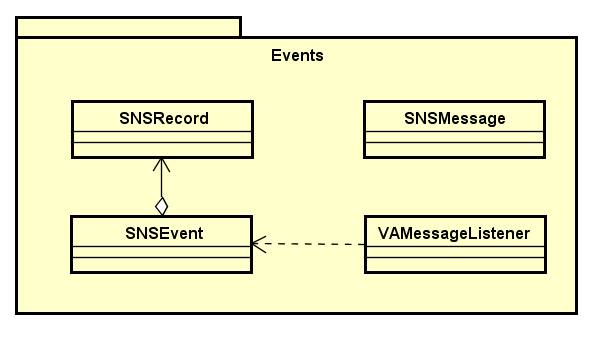
\includegraphics[width=\textwidth,height=\textheight,keepaspectratio]{images/diagrams/back-end/Official_Backend_0304/Events.png}
	\caption{Package Back-end::Events}
\end{figure}
\newpage

\paragraph{Classi}
\hypertarget{SNSMessage_label}{\subparagraph{SNSMessage}}
\begin{figure}[h]
	\centering
	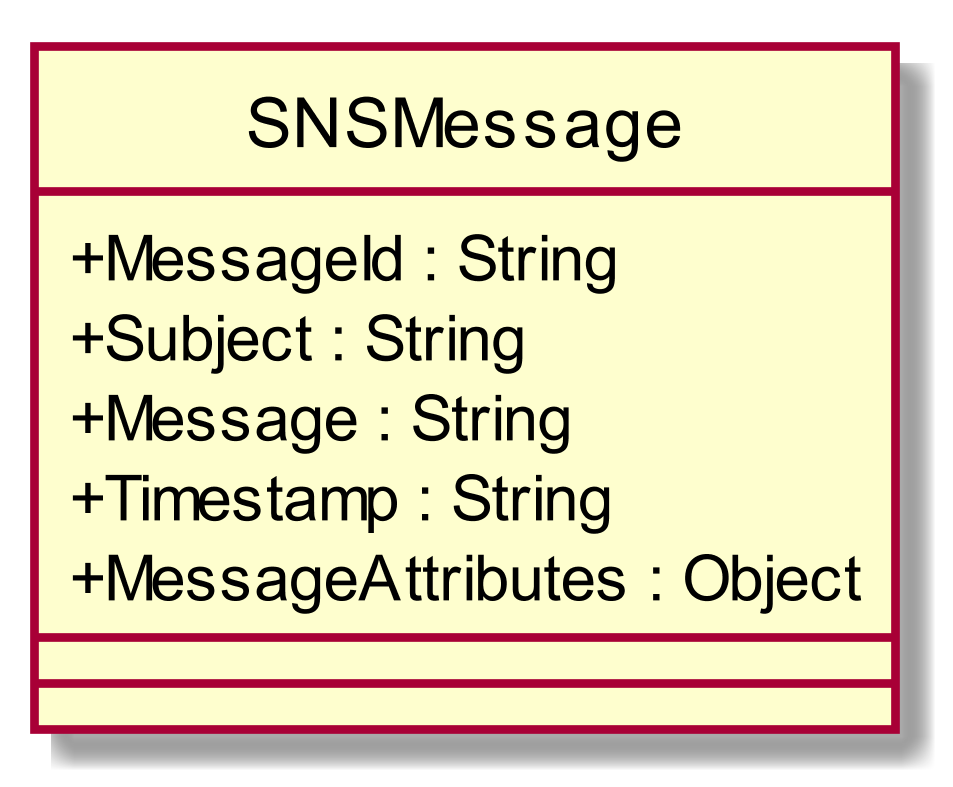
\includegraphics[width=0.35\textwidth,height=\textheight,keepaspectratio]{images/ClassSNSMessage.png}
	\caption{Back-end::Events::SNSMessage}
\end{figure}
\begin{itemize}
	\item \textbf{Nome}: \file{SNSMessage};
	\item \textbf{Tipo}: \file{Class};
	\item \textbf{Descrizione}: questa classe rappresenta un messaggio mandato da SNS in seguito ad un'interazione con l'assistente virtuale;
	\item \textbf{Utilizzo}: fornisce un meccanismo \gl{event-driven} per la gestione dei dati relativi alle interazioni col sistema.\\
	Per la relativa documentazione, consultare la pagina \url{http://docs.aws.amazon.com/sns/latest/dg/json-formats.html#http-subscription-confirmation-json};
	\item \textbf{Attributi}:
	\begin{itemize}
		\item[] \file{+ MessageId: String} \\
		Attributo contenente l'identificativo del messaggio;
		\item[] \file{+ Subject: String} \\
		Attributo contenente il Subject che dev'essere notificato dal sistema SNS;
		\item[] \file{+ Message: String} \\
		Attributo contenente il messaggio da pubblicare;
		\item[] \file{+ Timestamp: String} \\
		Attributo contenente il timestamp relativo al momento della pubblicazione del messaggio;
		\item[] \file{+ MessageAttributes: Object} \\
		Attributo contenente le coppie chiave-valore degli attributi del messaggio che è stato pubblicato su SNS;
	\end{itemize}
	\item \textbf{Relazioni con le altre classi}:
	\begin{itemize}
		\item IN \hyperlink{SNSRecord_label}{\file{SNSRecord}}
	\end{itemize}
\end{itemize}
\FloatBarrier

\hypertarget{SNSRecord_label}{\subparagraph{SNSRecord}}
\begin{figure}[h]
	\centering
	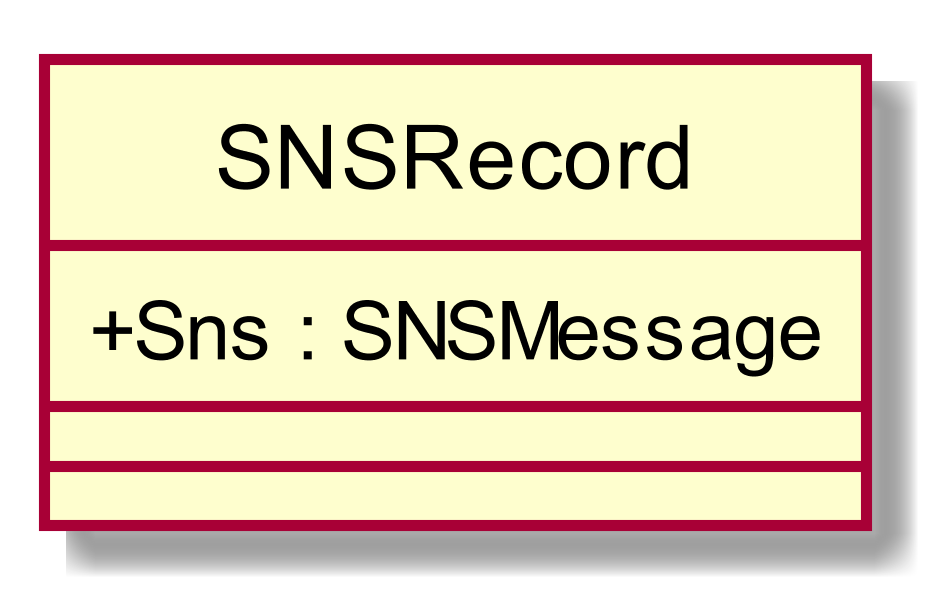
\includegraphics[width=0.35\textwidth,height=\textheight,keepaspectratio]{images/ClassSNSRecord.png}
	\caption{Back-end::Events::SNSRecord}
\end{figure}
\begin{itemize}
	\item \textbf{Nome}: \file{SNSRecord};
	\item \textbf{Tipo}: \file{Class};
	\item \textbf{Descrizione}: questa classe rappresenta uno dei records mandati da SNS ad una Lambda Function;
	\item \textbf{Utilizzo}: fornisce gli attributi di un record mandato da SNS ad una Lambda Function;
	\item \textbf{Attributi}:
	\begin{itemize}
		\item[] \file{+ Sns: SNSMessage} \\
		Attributo contenente i dati del messaggio pubblicato sul topic di SNS;
	\end{itemize}
	\item \textbf{Relazioni con le altre classi}:
	\begin{itemize}
		\item IN \hyperlink{SNSEvent_label}{\file{SNSEvent}}
		\item OUT \hyperlink{SNSMessage_label}{\file{SNSMessage}}
	\end{itemize}
\end{itemize}
\FloatBarrier

\hypertarget{VAMessageListener_label}{\subparagraph{VAMessageListener}}
\begin{figure}[h]
	\centering
	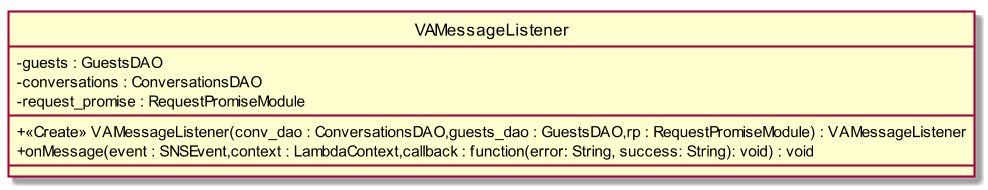
\includegraphics[width=\textwidth,height=\textheight,keepaspectratio]{images/ClassVAMessageListener.png}
	\caption{Back-end::Events::VAMessageListener}
\end{figure}
\begin{itemize}
	\item \textbf{Nome}: \file{VAMessageListener};
	\item \textbf{Tipo}: \file{Class};
	\item \textbf{Descrizione}: questa classe si occupa di registrare i dati relativi alle interazioni degli ospiti col nostro sistema;
	\item \textbf{Utilizzo}: fornisce un meccanismo per registrare i dialoghi che gli ospiti hanno con il sistema. Fornisce una Lambda Function che quando viene generato un evento \file{SNSMessage}, in seguito all'arrivo di una risposta da parte dell'assistente virtuale, si occupa di registrare i dati della relativa interazione tramite \file{ConversationsDAO}, ed eventualmente di aggiornare i dati relativi all'ospite utilizzando \file{GuestsDAO}. Inoltre si occupa di notificare la persona interessata dell'arrivo di un ospite e delle richieste da lui fatte;
	\item \textbf{Attributi}:
	\begin{itemize}
		\item[] \file{- guests: GuestsDAO} \\
		Attributo che permette di contattare il \file{GuestsDAO};
		\item[] \file{- conversations: ConversationsDAO} \\
		Attributo che permette di contattare il \file{ConversationsDAO};
		\item[] \file{- request\_promise: RequestPromiseModule} \\
		Attributo che rappresenta il modulo di Node.js utilizzato per le richieste HTTP;
	\end{itemize}
	\item \textbf{Metodi}:
	\begin{itemize}
		\item[] \file{+ <<Create>> VAMessageListener(conv\_dao: ConversationsDAO, guests\_dao\\: GuestsDAO, rp: RequestPromiseModule): VAMessageListener} \\		Costruttore che permette di effettuare la dependency injection dei moduli utilizzati da questa classe;\\
		Parametri:
		\begin{itemize}
			\item \file{conv\_dao: ConversationsDAO} \\
			Parametro contenente il \file{ConversationsDAO} del quale si vuole effettuare la dependency injection;
			\item \file{guests\_dao: GuestsDAO} \\
			Parametro contenente il \file{GuestDAO} del quale si vuole effettuare la dependency injection;
			\item \file{rp: RequestPromiseModule} \\
			Parametro contenente il \file{RequestPromiseModule} del quale si vuole effettuare la dependency injection;
		\end{itemize}
		\item[] \file{+ onMessage(event: SNSEvent, context: LambdaContext, callback: function\\(error: String, success: String): void): void} \\		Metodo che implementa la Lambda function che viene chiamata in seguito alla pubblicazione di un messaggio sul topic SNS. SNS chiama tale Lambda Function con un oggetto del tipo \file{SNSEvent}, il quale contiene al suo interno un array di \file{SNSRecord}. Questo array in realtà ha un unico oggetto, il quale al suo interno contiene l'\file{SNSMessage} inviato, in questo caso la rappresentazione in JSON di un oggetto di tipo \file{VAResponse}. \\
		Di seguito viene riportato un esempio dell'oggetto utilizzato.
		\begin{lstlisting}[language=json,firstnumber=1]
		{
		Records:
		[
		{
		Sns:
		{
		Message: '
		{
		"action":"nome.azione",
		"res":
		{
		"contexts":
		[
		{
		"name": "nome_contesto",
		"parameters":
		{
		"nome1": "valore",
		"nome2": "altro valore"
		}
		}
		],
		"data": Object,
		"text_request": "frase pronunciata dall'ospite",
		"text_response": "risposta dell'assistente"
		},
		"session_id": "idUnico.timestamp"
		}',
		MessageAttributes: {"key": "value", "key2": "value2"},
		MessageId: "stringa-contenente-id-del-messaggio",
		Subject: "oggetto del messaggio",
		Timestamp: "2017-03-26T20:39:48.599Z"
		}
		}
		]
		}
		\end{lstlisting}
		Il metodo si occupa, nel caso in cui siano noti i dati necessari ad identificare un ospite (nome e azienda di provenienza), di utilizzare \file{guests} e \file{conversations} per memorizzare l'interazione. Inoltre, dopo aver chiamato il microservizio \file{Rules} per richiedere le direttive da applicare, individua il canale nel quale inviare la notifica ed utilizzando il microservizio \file{Notification} manda un messaggio contenente i dati dell'interazione;\\
		Parametri:
		\begin{itemize}
			\item \file{event: SNSEvent} \\
			Parametro contenente i date relativi al messaggio pubblicato sul topic di SNS;
			\item \file{context: LambdaContext} \\
			Parametro contenente il \file{LambdaContext} relativo alla chiamata ricevuta dalla Lambda Function. Non verrà utilizzato all'interno della funzione;
			\item \file{callback: function(error: String, success: String): void} \\
			Parametro contenente la funzione di callback da utilizzare per comunicare al chiamante l'esito dell'esecuzione. Viene chiamata alla fine dell'esecuzione per comunicare che la chiamata è andata a buon fine con \file{null} come primo parametro. Nel caso in cui si sia verificato un errore, viene chiamata con un unico parametro contenente un messaggio di errore;
		\end{itemize}
	\end{itemize}
	\item \textbf{Relazioni con le altre classi}:
	\begin{itemize}
		\item OUT \hyperlink{<<interface>> ConversationsDAO_label}{\file{<<interface>> ConversationsDAO}}
		\item OUT \hyperlink{<<interface>> GuestsDAO_label}{\file{<<interface>> GuestsDAO}}
		\item OUT \hyperlink{SNSEvent_label}{\file{SNSEvent}}
	\end{itemize}
\end{itemize}
\FloatBarrier

\newpage \subsubsection{Back-end::Guests}
Package contenente le classi relative ai Guests del sistema.
\begin{figure}[h] \centering 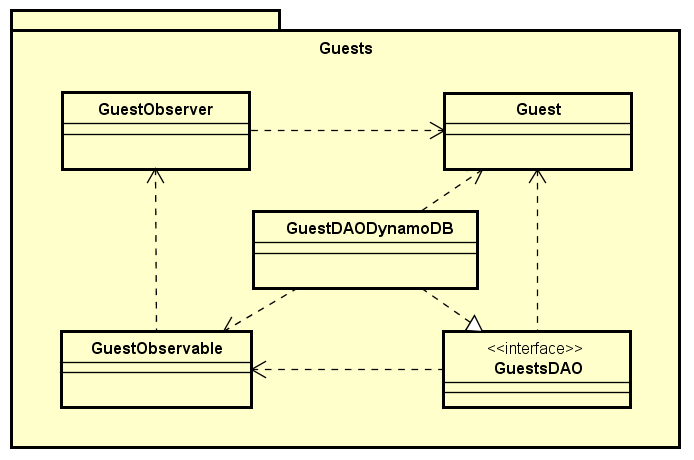
\includegraphics[width=\textwidth,height=\textheight,keepaspectratio]{images/diagrams/back-end/Official_Backend_0304/Guest.png}
	\caption{Package Back-end::Guests}
\end{figure}
\newpage

\paragraph{Classi}
\hypertarget{ GuestsDAO_label}{\subparagraph{ GuestsDAO}}
\begin{figure}[h]
	\centering
	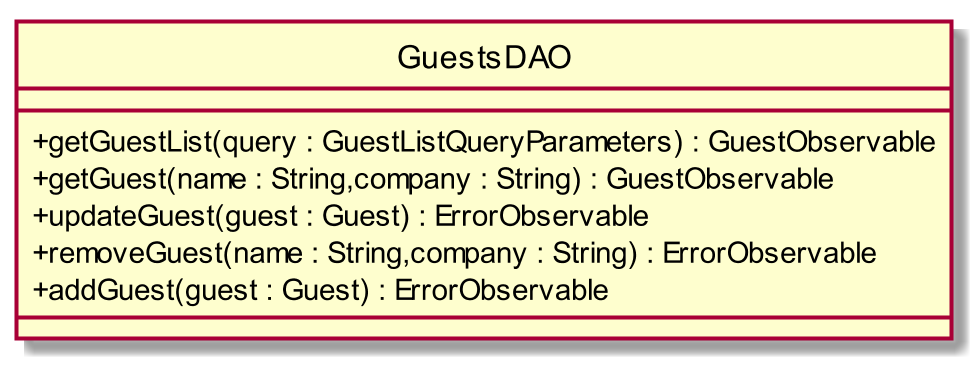
\includegraphics[width=0.55\textwidth,height=\textheight,keepaspectratio]{images/ClassGuestsDAO.png}
	\caption{Back-end::Guests:: GuestsDAO}
\end{figure}
\begin{itemize}
	\item \textbf{Nome}: \file{ GuestsDAO};
	\item \textbf{Tipo}: \file{Interface};
	\item \textbf{Descrizione}: questa interfaccia si occupa di astrarre le modalità d'interazione al database contenente gli ospiti conosciuti;
	\item \textbf{Utilizzo}: fornisce i metodi per accedere al database contenente i dati relativi agli ospiti conosciuti, senza conoscerne le modalità di implementazioni e di persistenza di quest'ultimo. Permette operazioni di lettura, scrittura e rimozione di ospiti conosciuti;
	\item \textbf{Figlio}: \file{GuestsDAODynamoDB};
	\item \textbf{Metodi}:
	\begin{itemize}
		\item[] \file{+ getGuestList(): GuestObservable} \\		L'\file{Observable} restituito manderà agli \file{Observer} gli ospiti ottenuti, uno alla volta, e poi chiama il loro metodo \file{complete}. Nel caso in cui si verifichi un errore, gli \file{Observer} iscritti verranno notificati tramite la chiamate del loro metodo \file{error} con i dati relativi all'errore verificatosi;\\
		\item[] \file{+ getGuest(name: String, company: String): GuestObservable} \\		Metodo che permette di ottenere un ospite a partire dal nome e l'azienda di provenienza. \\
		L'\file{Observable} restituito riceverà l'oggetto rappresentante tale \file{Guest}, e verrà completato. Nel caso in cui l'ospite richiesto non sia presente nel database, gli \file{Observer} interessati non riceveranno alcun valore, ma verranno notificati tramite la chiamata del loro metodo \file{error};\\
		Parametri:
		\begin{itemize}
			\item \file{name: String} \\
			Parametro contenente il nome dell'ospite;
			\item \file{company: String} \\
			Parametro contenente l'azienda di provenienza dell'ospite;
		\end{itemize}
		\item[] \file{+ updateGuest(guest: Guest): ErrorObservable} \\		Metodo che permette di aggiornare un ospite.  L'\file{Observable} restituito non riceverà alcun valore, ma verrà completato in caso di aggiunta dell'ospite avvenuta con successo. In caso di errore durante l'aggiunta dell'ospite, gli \file{Observer} interessati verranno notificati tramite la chiamata del loro metodo \file{error} con i dati relativi all'errore verificatosi;\\
		Parametri:
		\begin{itemize}
			\item \file{guest: Guest} \\
			Parametro contenente l'ospite da aggiornare;
		\end{itemize}
		\item[] \file{+ removeGuest(name: String, company: String): ErrorObservable} \\\\		Metodo che permette di eliminare un ospite dal database, a partire dal suo nome e azienda di provenienza.  L'\file{Observable} restituito non riceverà alcun valore, ma verrà completato in caso di eliminazione  dell'ospite avvenuta con successo. In caso di errore durante l'eliminazione dell'ospite, gli \file{Observer} interessati verranno notificati tramite la chiamata del loro metodo \file{error} con i dati relativi all'errore verificatosi;\\
		Parametri:
		\begin{itemize}
			\item \file{name: String} \\
			Parametro contenente il nome dell'ospite;
			\item \file{company: String} \\
			Parametro contenente l'azienda di provenienza dell'ospite;
		\end{itemize}
		\item[] \file{+ addGuest(guest: Guest): ErrorObservable} \\		Metodo che permette di aggiungere un ospite al database.  L'\file{Observable} restituito non riceverà alcun valore, ma verrà completato in caso di aggiunta dell'ospite avvenuta con successo. In caso di errore durante l'aggiunta dell'ospite, gli \file{Observer} interessati verranno notificati tramite la chiamata del loro metodo \file{error} con i dati relativi all'errore verificatosi;\\
		Parametri:
		\begin{itemize}
			\item \file{guest: Guest} \\
			Parametro contenente l'ospite da aggiungere;
		\end{itemize}
	\end{itemize}
	\item \textbf{Relazioni con le altre classi}:
	\begin{itemize}
		\item IN \hyperlink{ConversationWebhookService_label}{\file{ConversationWebhookService}}
		\item IN \hyperlink{VAMessageListener_label}{\file{VAMessageListener}}
		\item OUT \hyperlink{Guest_label}{\file{Guest}}
		\item OUT \hyperlink{GuestObservable_label}{\file{GuestObservable}}
		\item OUT \hyperlink{ErrorObservable_label}{\file{ErrorObservable}}
	\end{itemize}
\end{itemize}
\FloatBarrier

\hypertarget{Guest_label}{\subparagraph{Guest}}
\begin{figure}[h]
	\centering
	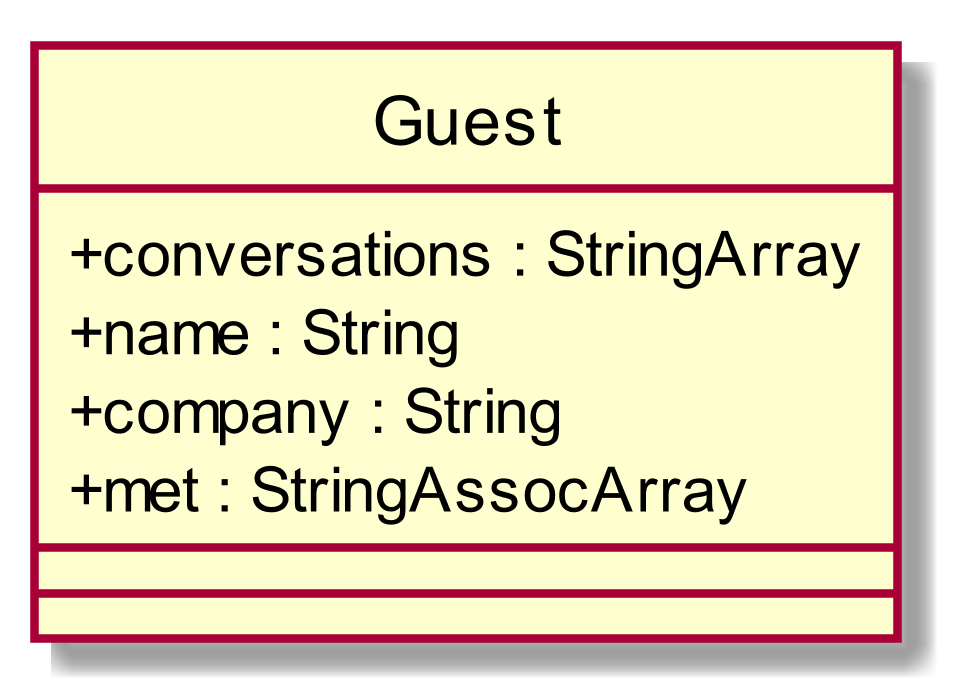
\includegraphics[width=0.35\textwidth,height=\textheight,keepaspectratio]{images/ClassGuest.png}
	\caption{Back-end::Guests::Guest}
\end{figure}
\begin{itemize}
	\item \textbf{Nome}: \file{Guest};
	\item \textbf{Tipo}: \file{Class};
	\item \textbf{Descrizione}: questa classe si occupa di rappresentare e organizzare gli attributi relativi ad un ospite conosciuto, i quali dovranno essere salvati nel database;
	\item \textbf{Utilizzo}: fornisce gli attributi relativi ad un ospite;
	\item \textbf{Attributi}:
	\begin{itemize}
		\item[] \file{+ conversations: StringArray} \\
		Attributo contenente l'array delle conversazioni avute con l'ospite;
		\item[] \file{+ name: String} \\
		Attributo contenente il nome dell'ospite;
		\item[] \file{+ company: String} \\
		Attributo contenente l'azienda di provenienza dell'ospite;
		\item[] \file{+ met: StringAssocArray} \\
		Attributo contenente l'array associativo del numero di volte che una persona è stata accolta. La chiave di questo array associativo è il nome del membro dell'azienda;
	\end{itemize}
	\item \textbf{Relazioni con le altre classi}:
	\begin{itemize}
		\item IN \hyperlink{<<interface>> GuestsDAO_label}{\file{<<interface>> GuestsDAO}}
		\item IN \hyperlink{GuestObserver_label}{\file{GuestObserver}}
		\item IN \hyperlink{GuestsDAODynamoDB_label}{\file{GuestsDAODynamoDB}}
	\end{itemize}
\end{itemize}
\FloatBarrier

\hypertarget{GuestObservable_label}{\subparagraph{GuestObservable}}
\begin{figure}[h]
	\centering
	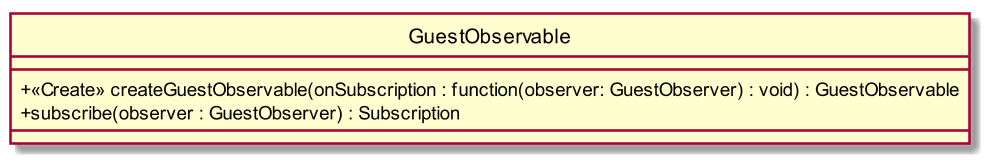
\includegraphics[width=\textwidth,height=\textheight,keepaspectratio]{images/ClassGuestObservable.png}
	\caption{Back-end::Guests::GuestObservable}
\end{figure}
\begin{itemize}
	\item \textbf{Nome}: \file{GuestObservable};
	\item \textbf{Tipo}: \file{Class};
	\item \textbf{Descrizione}: questa classe implementa un \file{Observable} che permette l'iscrizione di \file{GuestObserver};
	\item \textbf{Utilizzo}: fornisce i meccanismi necessari per il passaggio di una serie di \file{Guest} ad un \file{Observer} interessato;
	\item \textbf{Padre}: \file{Observable};
	\item \textbf{Metodi}:
	\begin{itemize}
		\item[] \file{+ <<Create>> createGuestObservable(onSubscription: function(observer\\: GuestObserver) : void): GuestObservable} \\		Constructor di \file{GuestObservable};\\
		Parametri:
		\begin{itemize}
			\item \file{onSubscription: function(observer: GuestObserver) : void} \\
			Funzione che verrà eseguita quando un \file{Observer} si iscrive all'\file{Observable}. Si occupa di passare i dati all'\file{Observer}, chiamando il metodo \file{next(guest: Guest)}. Quando non ci sono più dati da restituire, si occupa di chiamare il metodo \file{complete}. Nel caso in cui si verificasse un errore, si occupa di chiamare il metodo \file{error(err: Object)} con i dati relativi all'errore verificatosi;
		\end{itemize}
		\item[] \file{+ subscribe(observer: GuestObserver): Subscription} \\		Metodo che permette ad un \file{GuestObserver} interessato di iscriversi a questo \file{Observable};\\
		Parametri:
		\begin{itemize}
			\item \file{observer: GuestObserver} \\
			\file{Observer} che si vuole iscrivere;
		\end{itemize}
	\end{itemize}
	\item \textbf{Relazioni con le altre classi}:
	\begin{itemize}
		\item IN \hyperlink{<<interface>> GuestsDAO_label}{\file{<<interface>> GuestsDAO}}
		\item IN \hyperlink{GuestsDAODynamoDB_label}{\file{GuestsDAODynamoDB}}
		\item OUT \hyperlink{GuestObserver_label}{\file{GuestObserver}}
	\end{itemize}
\end{itemize}
\FloatBarrier

\hypertarget{GuestObserver_label}{\subparagraph{GuestObserver}}
\begin{figure}[h]
	\centering
	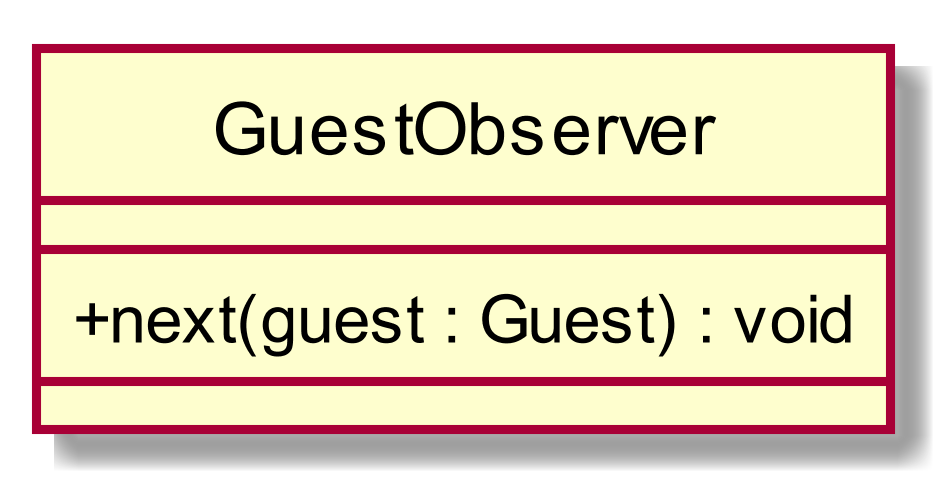
\includegraphics[width=0.35\textwidth,height=\textheight,keepaspectratio]{images/ClassGuestObserver.png}
	\caption{Back-end::Guests::GuestObserver}
\end{figure}
\begin{itemize}
	\item \textbf{Nome}: \file{GuestObserver};
	\item \textbf{Tipo}: \file{Class};
	\item \textbf{Descrizione}: classe che rappresenta un \file{Observer} che si aspetta oggetti di tipo \file{Guest};
	\item \textbf{Utilizzo}: ridefinisce il metodo \file{next} della classe \file{ObserverAdapter}, in modo che riceva dati di tipo \file{Guest};
	\item \textbf{Metodi}:
	\begin{itemize}
		\item[] \file{+ next(guest: Guest): void} \\		Metodo che permette agli \file{Observable} di notificare l'\file{Observer} con dati di tipo \file{Guest}. Definisce inoltre le operazioni che l'\file{Observer} compierà all'arrivo di tali dati;\\
		Parametri:
		\begin{itemize}
			\item \file{guest: Guest} \\
			Parametro contenente il \file{Guest} mandato dall'\file{Observable};
		\end{itemize}
	\end{itemize}
	\item \textbf{Relazioni con le altre classi}:
	\begin{itemize}
		\item IN \hyperlink{GuestObservable_label}{\file{GuestObservable}}
		\item OUT \hyperlink{Guest_label}{\file{Guest}}
	\end{itemize}
\end{itemize}
\FloatBarrier

\hypertarget{GuestsDAODynamoDB_label}{\subparagraph{GuestsDAODynamoDB}}
\begin{figure}[h]
	\centering
	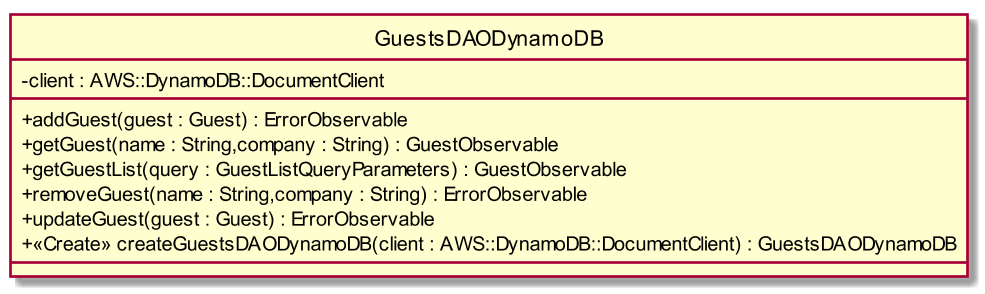
\includegraphics[width=0.80\textwidth,height=\textheight,keepaspectratio]{images/ClassGuestsDAODynamoDB.png}
	\caption{Back-end::Guests::GuestsDAODynamoDB}
\end{figure}
\begin{itemize}
	\item \textbf{Nome}: \file{GuestsDAODynamoDB};
	\item \textbf{Tipo}: \file{Class};
	\item \textbf{Descrizione}: classe che si occupa di implementare l'interfaccia \file{GuestsDAO}, utilizzando un database DynamoDB come supporto per la memorizzazione dei dati;
	\item \textbf{Utilizzo}: implementa i metodi dell'interfaccia \file{GuestsDAO} interrogando un database DynamoDB. Utilizza \file{AWS::DynamoDB::DocumentClient} per l'accesso al database. La dependency injection dell'oggetto \file{AWS::DynamoDB} viene fatta utilizzando il costruttore;
	\item \textbf{Padre}: \file{<<interface>> GuestsDAO};
	\item \textbf{Attributi}:
	\begin{itemize}
		\item[] \file{- client: AWS::DynamoDB::DocumentClient} \\
		Attributo contenente un riferimento al modulo di Node.js utilizzato per l'accesso al database DynamoDB contenente la tabella degli ospiti;
	\end{itemize}
	\item \textbf{Metodi}:
	\begin{itemize}
		\item[] \file{+ addGuest(guest: Guest): ErrorObservable} \\		Implementazione del metodo definito nell'interfaccia \file{GuestsDAO}. Utilizza il metodo \file{put} del \file{DocumentClient} per aggiungere l'ospite al database;\\
		Parametri:
		\begin{itemize}
			\item \file{guest: Guest} \\
			Parametro contenente l'ospite da aggiungere;
		\end{itemize}
		\item[] \file{+ getGuest(name: String, company: String): GuestObservable} \\		Implementazione del metodo definito nell'interfaccia \file{GuestsDAO}. Utilizza il metodo \file{get} del \file{DocumentClient} per ottenere i dati relativi ad un \file{Guest} dal database;\\
		Parametri:
		\begin{itemize}
			\item \file{name: String} \\
			Parametro contenente il nome dell'ospite;
			\item \file{company: String} \\
			Parametro contenente l'azienda di provenienza dell'ospite;
		\end{itemize}
		\item[] \file{+ getGuestList(): GuestObservable} \\		Implementazione del metodo dell'interfaccia \file{GuestsDAO}. Utilizza il metodo \file{scan} del \file{DocumentClient} per ottenere la lista degli ospiti dal database;\\
		\item[] \file{+ removeGuest(name: String, company: String): ErrorObservable} \\\\		Implementazione del metodo dell'interfaccia \file{GuestsDAO}. Utilizza il metodo \file{delete} del \file{DocumentClient} per eliminare un ospite dal database;\\
		Parametri:
		\begin{itemize}
			\item \file{name: String} \\
			Parametro contenente il nome dell'ospite;
			\item \file{company: String} \\
			Parametro contenente l'azienda di provenienza dell'ospite;
		\end{itemize}
		\item[] \file{+ updateGuest(guest: Guest): ErrorObservable} \\		Implementazione del metodo dell'interfaccia \file{GuestsDAO}. Utilizza il metodo \file{update} del \file{DocumentClient} per aggiornare i dati relativi ad un ospite presenti all'interno del database;\\
		Parametri:
		\begin{itemize}
			\item \file{guest: Guest} \\
			Parametro contenente l'ospite da aggiornare;
		\end{itemize}
		\item[] \file{+ <<Create>> createGuestsDAODynamoDB(client: AWS::DynamoDB::DocumentClient)\\: GuestsDAODynamoDB} \\		Constructor della classe \file{GuestsDAODynamoDB}. Permette di effettuare la dependency injection di \file{AWS::DynamoDB};\\
		Parametri:
		\begin{itemize}
			\item \file{client: AWS::DynamoDB::DocumentClient} \\
			Parametro contenente un riferimento al modulo di Node.js da utilizzare per l'accesso al database DynamoDB contenente la tabella degli ospiti;
		\end{itemize}
	\end{itemize}
	\item \textbf{Relazioni con le altre classi}:
	\begin{itemize}
		\item OUT \hyperlink{Guest_label}{\file{Guest}}
		\item OUT \hyperlink{GuestObservable_label}{\file{GuestObservable}}
		\item OUT \hyperlink{ErrorObservable_label}{\file{ErrorObservable}}
	\end{itemize}
\end{itemize}
\FloatBarrier

\newpage \subsubsection{Back-end::Members}
Package contenente le classi relative ai membri del sistema.
\begin{figure}[h] \centering 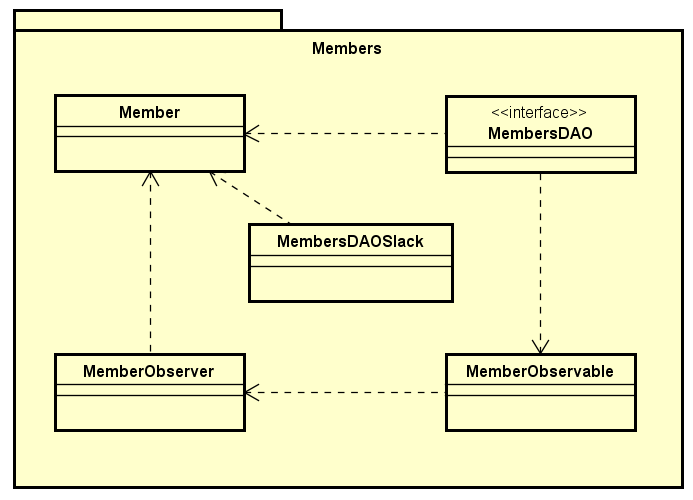
\includegraphics[width=\textwidth,height=\textheight,keepaspectratio]{images/diagrams/back-end/Official_Backend_0304/Member.png}
	\caption{Package Back-end::Members}
\end{figure}
\newpage
\paragraph{Classi}
\hypertarget{ MembersDAO_label}{\subparagraph{ MembersDAO}}
\begin{figure}[h]
	\centering
	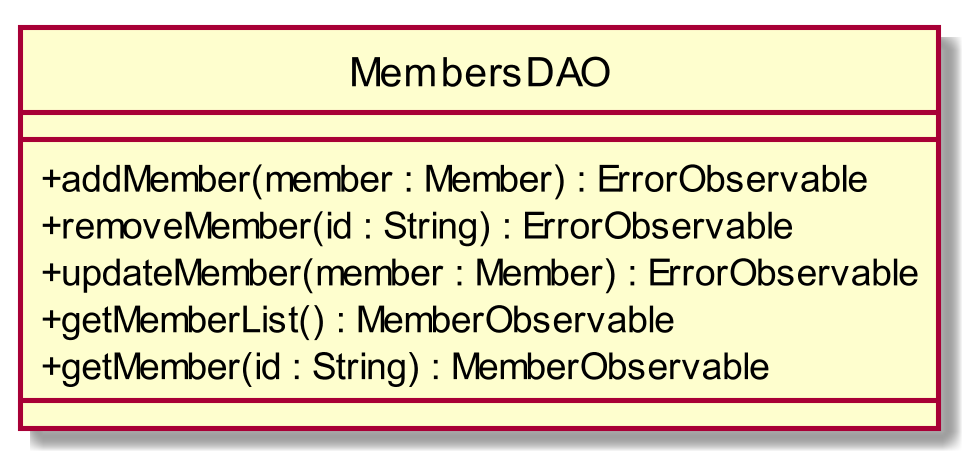
\includegraphics[width=0.50\textwidth,height=\textheight,keepaspectratio]{images/ClassMembersDAO.png}
	\caption{Back-end::Members:: MembersDAO}
\end{figure}
\begin{itemize}
	\item \textbf{Nome}: \file{ MembersDAO};
	\item \textbf{Tipo}: \file{Interface};
	\item \textbf{Descrizione}: questa classe si occupa di astrarre le modalità d'accesso ai dati relativi ai membri dell'azienda;
	\item \textbf{Utilizzo}: fornisce i meccanismi necessare per inserire, modificare, rimuovere ed ottenere i dati relativi ai membri dell'azienda;
	\item \textbf{Figlio}: \file{MembersDAOSlack};
	\item \textbf{Metodi}:
	\begin{itemize}
		\item[] \file{+ addMember(member: Member): ErrorObservable} \\		Metodo che permette di aggiungere un membro;\\
		Parametri:
		\begin{itemize}
			\item \file{member: Member} \\
			Membro da aggiungere;
		\end{itemize}
		\item[] \file{+ removeMember(id: String): ErrorObservable} \\		Metodo che permette di rimuovere un membro;\\
		Parametri:
		\begin{itemize}
			\item \file{id: String} \\
			Stringa identificativa del membro che si vuole rimuovere;
		\end{itemize}
		\item[] \file{+ updateMember(member: Member): ErrorObservable} \\		Metodo che permette di modificare un utente inserito in precedenza;\\
		Parametri:
		\begin{itemize}
			\item \file{member: Member} \\
			Parametro contenente i dati relativi al membro che si vuole modificare;
		\end{itemize}
		\item[] \file{+ getMemberList(): MemberObservable} \\		Metodo che permette di ottenere la lista dei membri inseriti;\\
		\item[] \file{+ getMember(id: String): MemberObservable} \\		Metodo che permette di ottenere i dati relativi ad un determinato membro;\\
		Parametri:
		\begin{itemize}
			\item \file{id: String} \\
			Parametro contenete la stringa identificativa del membro del quale si vogliono ottenere i dati;
		\end{itemize}
	\end{itemize}
	\item \textbf{Relazioni con le altre classi}:
	\begin{itemize}
		\item OUT \hyperlink{MemberObservable_label}{\file{MemberObservable}}
		\item OUT \hyperlink{Member_label}{\file{Member}}
		\item OUT \hyperlink{ErrorObservable_label}{\file{ErrorObservable}}
	\end{itemize}
\end{itemize}
\FloatBarrier

\hypertarget{Member_label}{\subparagraph{Member}}
\begin{figure}[h]
	\centering
	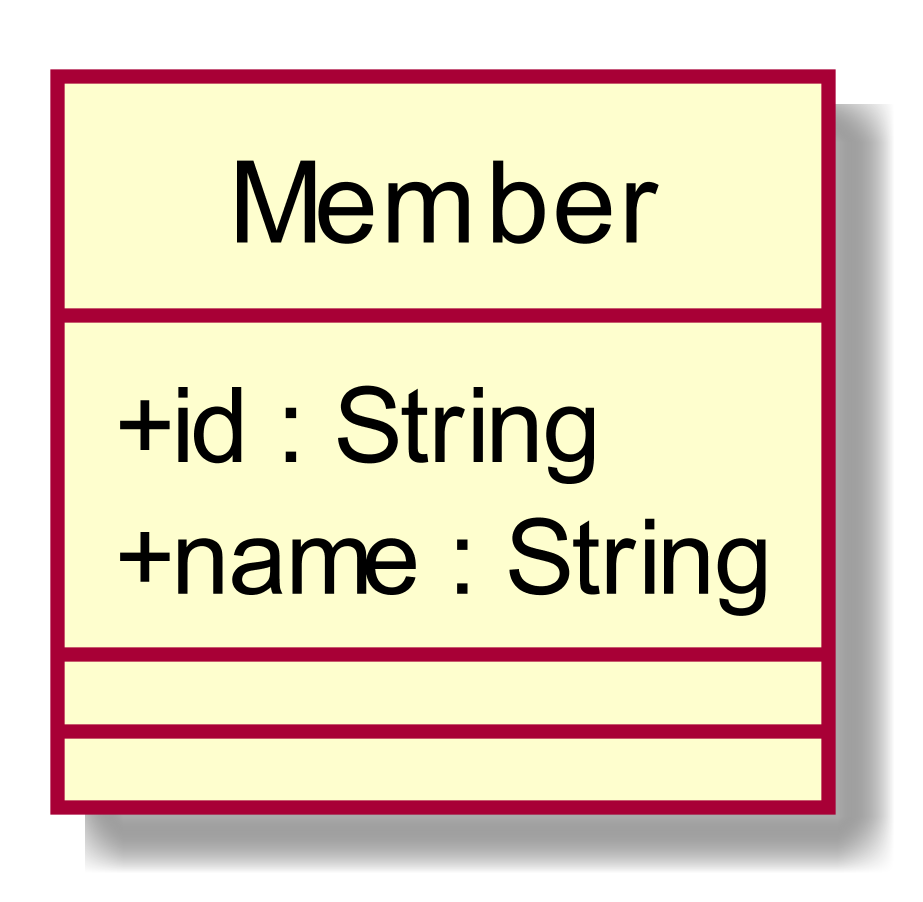
\includegraphics[width=0.35\textwidth,height=\textheight,keepaspectratio]{images/ClassMember.png}
	\caption{Back-end::Members::Member}
\end{figure}
\begin{itemize}
	\item \textbf{Nome}: \file{Member};
	\item \textbf{Tipo}: \file{Class};
	\item \textbf{Descrizione}: questa classe si occupa di raggruppare le informazioni relative ad un membro dell'azienda;
	\item \textbf{Utilizzo}: fornisce l'accesso ai dati relativi ad un membro dell'azienda;
	\item \textbf{Attributi}:
	\begin{itemize}
		\item[] \file{+ id: String} \\
		Stringa contenente l'id del canale Slack del membro dell'azienda;
		\item[] \file{+ name: String} \\
		Nome del membro dell'azienda;
	\end{itemize}
	\item \textbf{Relazioni con le altre classi}:
	\begin{itemize}
		\item IN \hyperlink{<<interface>> MembersDAO_label}{\file{<<interface>> MembersDAO}}
		\item IN \hyperlink{MemberObserver_label}{\file{MemberObserver}}
		\item IN \hyperlink{MembersDAOSlack_label}{\file{MembersDAOSlack}}
	\end{itemize}
\end{itemize}
\FloatBarrier

\hypertarget{MemberObservable_label}{\subparagraph{MemberObservable}}
\begin{figure}[h]
	\centering
	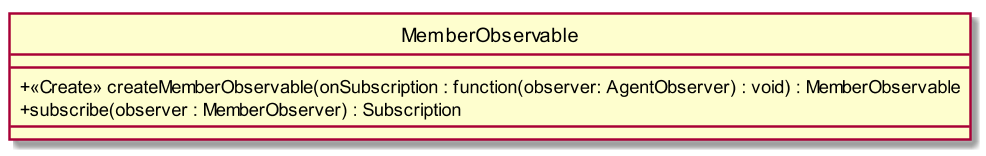
\includegraphics[width=\textwidth,height=\textheight,keepaspectratio]{images/ClassMemberObservable.png}
	\caption{Back-end::Members::MemberObservable}
\end{figure}
\begin{itemize}
	\item \textbf{Nome}: \file{MemberObservable};
	\item \textbf{Tipo}: \file{Class};
	\item \textbf{Descrizione}: questa classe implementa un \file{Observable} che permette l'iscrizione di \file{MemberObserver};
	\item \textbf{Utilizzo}: fornisce i meccanismi necessari per il passaggio di una serie di \file{Member} ad un \file{Observer} interessato;
	\item \textbf{Padre}: \file{Observable};
	\item \textbf{Metodi}:
	\begin{itemize}
		\item[] \file{+ <<Create>> createMemberObservable(onSubscription: function(observer\\: AgentObserver) : void): MemberObservable} \\		Constructor di \file{MemberObservable};\\
		Parametri:
		\begin{itemize}
			\item \file{onSubscription: function(observer: AgentObserver) : void} \\
			Funzione che verrà eseguita quando un \file{Observer} si iscrive all'\file{Observable}. Si occupa di passare i dati all'\file{Observer}, chiamando il metodo \file{next(member: Member)}. Quando non ci sono più dati da restituire, si occupa di chiamare il metodo \file{complete}. Nel caso in cui si verificasse un errore, si occupa di chiamare il metodo \file{error(err: Object)} con i dati relativi all'errore verificatosi;
		\end{itemize}
		\item[] \file{+ subscribe(observer: MemberObserver): Subscription} \\		Metodo che permette ad uno \file{MemberObserver} interessato di iscriversi a questo \file{Observable};\\
		Parametri:
		\begin{itemize}
			\item \file{observer: MemberObserver} \\
			\file{Observer} che si vuole iscrivere;
		\end{itemize}
	\end{itemize}
	\item \textbf{Relazioni con le altre classi}:
	\begin{itemize}
		\item IN \hyperlink{<<interface>> MembersDAO_label}{\file{<<interface>> MembersDAO}}
		\item OUT \hyperlink{MemberObserver_label}{\file{MemberObserver}}
	\end{itemize}
\end{itemize}
\FloatBarrier

\hypertarget{MemberObserver_label}{\subparagraph{MemberObserver}}
\begin{figure}[h]
	\centering
	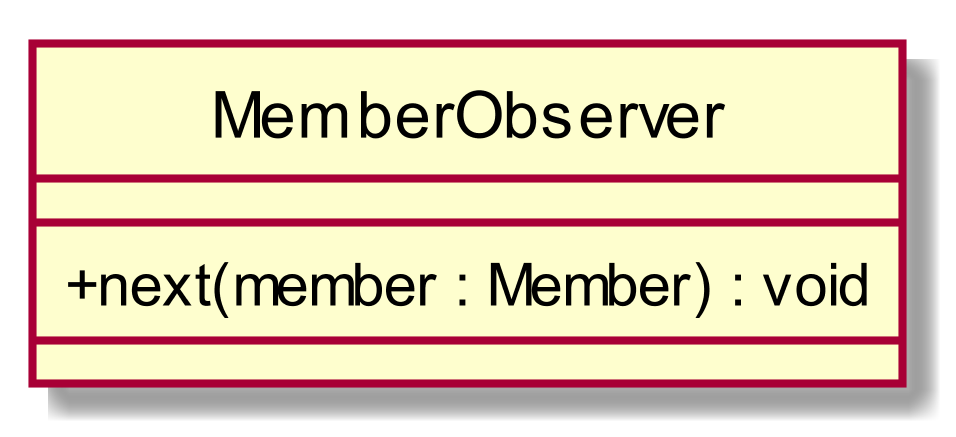
\includegraphics[width=0.35\textwidth,height=\textheight,keepaspectratio]{images/ClassMemberObserver.png}
	\caption{Back-end::Members::MemberObserver}
\end{figure}
\begin{itemize}
	\item \textbf{Nome}: \file{MemberObserver};
	\item \textbf{Tipo}: \file{Class};
	\item \textbf{Descrizione}: classe che rappresenta un \file{Observer} che si aspetta dati di tipo \file{Member};
	\item \textbf{Utilizzo}: ridefinisce il metodo \file{next} della classe \file{ObserverAdapter}, in maniera tale che accetti dati di tipo \file{Member};
	\item \textbf{Metodi}:
	\begin{itemize}
		\item[] \file{+ next(member: Member): void} \\		Metodo che permette agli \file{Observable} di notificare l'\file{Observer} con dati di tipo \file{Member}. Definisce inoltre le operazioni che l'\file{Observer} compierà all'arrivo di tali dati;\\
		Parametri:
		\begin{itemize}
			\item \file{member: Member} \\
			Parametro contenente l'\file{Member} mandato dall'\file{Observable};
		\end{itemize}
	\end{itemize}
	\item \textbf{Relazioni con le altre classi}:
	\begin{itemize}
		\item IN \hyperlink{MemberObservable_label}{\file{MemberObservable}}
		\item OUT \hyperlink{Member_label}{\file{Member}}
	\end{itemize}
\end{itemize}
\FloatBarrier

\hypertarget{MembersDAOSlack_label}{\subparagraph{MembersDAOSlack}}
\begin{figure}[h]
	\centering
	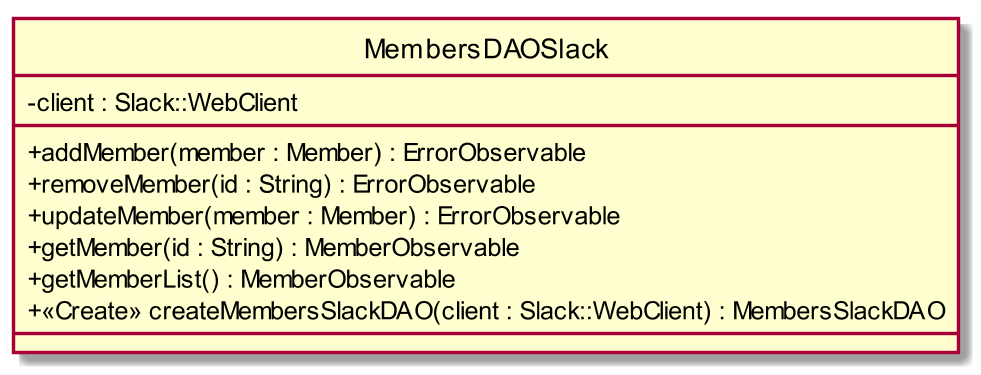
\includegraphics[width=0.60\textwidth,height=\textheight,keepaspectratio]{images/ClassMembersDAOSlack.png}
	\caption{Back-end::Members::MembersDAOSlack}
\end{figure}
\begin{itemize}
	\item \textbf{Nome}: \file{MembersDAOSlack};
	\item \textbf{Tipo}: \file{Class};
	\item \textbf{Descrizione}: questa classe implementa \file{MembersDAO}, ottenendo i dati da Slack;
	\item \textbf{Utilizzo}: implementa i metodi definiti dall'interfaccia, utilizzando \file{Slack::WebClient} per recuperare i dati relativi ai membri dell'azienda;
	\item \textbf{Padre}: \file{<<interface>> MembersDAO};
	\item \textbf{Attributi}:
	\begin{itemize}
		\item[] \file{- client: Slack::WebClient} \\
		Questo attributo è utilizzato per interrogare le API Web di Slack;
	\end{itemize}
	\item \textbf{Metodi}:
	\begin{itemize}
		\item[] \file{+ addMember(member: Member): ErrorObservable} \\		Implementazione del metodo del'interfaccia. L'\file{Observable} restituita genererà sempre un errore, in quanto non è possibile aggiungere membri;\\
		Parametri:
		\begin{itemize}
			\item \file{member: Member} \\
			Parametro contenente i dati relativi al membro che si vuole aggiungere;
		\end{itemize}
		\item[] \file{+ removeMember(id: String): ErrorObservable} \\		Implementazione del metodo del'interfaccia. L'\file{Observable} restituita genererà sempre un errore, in quanto non è possibile rimuovere membri;\\
		Parametri:
		\begin{itemize}
			\item \file{id: String} \\
			Parametro contenente la stringa identificativa del membro che si vuole eliminare;
		\end{itemize}
		\item[] \file{+ updateMember(member: Member): ErrorObservable} \\		Implementazione del metodo del'interfaccia. L'\file{Observable} restituita genererà sempre un errore, in quanto non è possibile aggiornare i dati dei membri;\\
		Parametri:
		\begin{itemize}
			\item \file{member: Member} \\
			Parametro contenente i dati relativi al membro che si vuole aggiornare;
		\end{itemize}
		\item[] \file{+ getMember(id: String): MemberObservable} \\		Implementazione del metodo del'interfaccia. Utilizza il metodo \file{users.info} per ottenere le informazioni necessarie da Slack;\\
		Parametri:
		\begin{itemize}
			\item \file{id: String} \\
			parametro contenente la stringa identificativa del membro del quale si vogliono ottenere i dati;
		\end{itemize}
		\item[] \file{+ getMemberList(): MemberObservable} \\		Implementazione del metodo del'interfaccia. Utilizza il metodo \file{users.list} per ottenere le informazioni necessarie da Slack;\\
		\item[] \file{+ <<Create>> createMembersSlackDAO(client: Slack::WebClient): MembersSlackDAO}\\ \\		Costruttore che permette di effettuare la dependency injection di \file{Slack::WebClient};\\
		Parametri:
		\begin{itemize}
			\item \file{client: Slack::WebClient} \\
			Parametro contenente un riferimento all'oggetto di tipo \file{Slack::WebClient} del quale si vuole effettuare la dependency injection;
		\end{itemize}
	\end{itemize}
	\item \textbf{Relazioni con le altre classi}:
	\begin{itemize}
		\item OUT \hyperlink{Member_label}{\file{Member}}
		\item OUT \hyperlink{ErrorObservable_label}{\file{ErrorObservable}}
	\end{itemize}
\end{itemize}
\FloatBarrier

\newpage \subsubsection{Back-end::Notifications}
Package contenente le classi e le interfacce che realizzano il microservizio relativo alla gestione delle notifiche da inviare alla persona desiderata su una certa piattaforma di messaggistica.
\begin{figure}[h] \centering 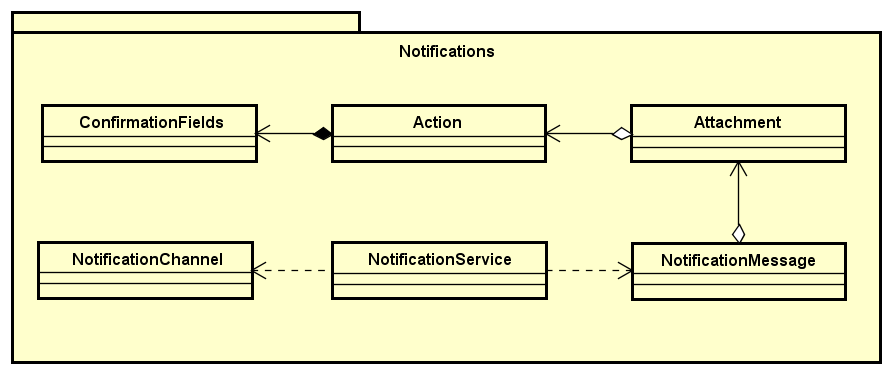
\includegraphics[width=\textwidth,height=\textheight,keepaspectratio]{images/diagrams/back-end/Official_Backend_0304/Notifications.png}
	\caption{Package Back-end::Notifications}
\end{figure}
\newpage

\paragraph{Classi}
\hypertarget{Action_label}{\subparagraph{Action}}
\begin{figure}[h]
	\centering
	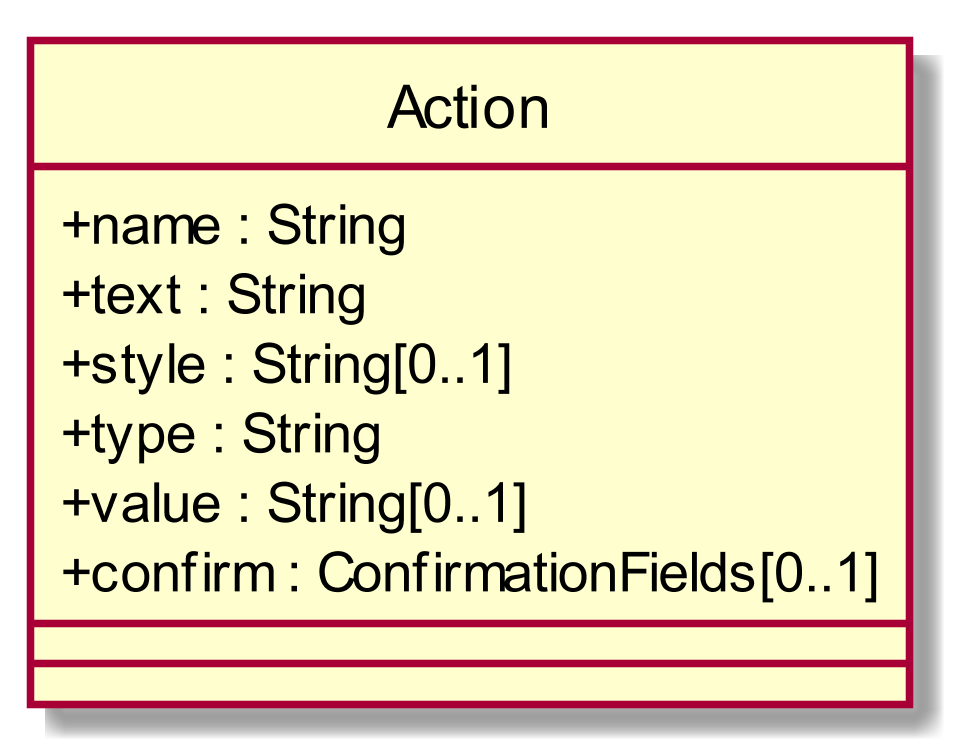
\includegraphics[width=0.35\textwidth,height=\textheight,keepaspectratio]{images/ClassAction.png}
	\caption{Back-end::Notifications::Action}
\end{figure}
\begin{itemize}
	\item \textbf{Nome}: \file{Action};
	\item \textbf{Tipo}: \file{Class};
	\item \textbf{Descrizione}: questa classe si occupa di rappresentare e organizzare gli attributi relativi ad una \file{Action} come descritto nelle API di Slack. Rappresenta un button in un messaggio Slack;
	\item \textbf{Utilizzo}: fornisce gli attributi di una \file{Action}. La classe \file{Attachment} ne contiene un array.
	Per la relativa documentazione, consultare la pagina \url{https://api.slack.com/docs/message-buttons}  (visitato in data 2017-03-21);
	\item \textbf{Attributi}:
	\begin{itemize}
		\item[] \file{+ name: String} \\
		Attributo contenente il nome dell'azione. Se ci sono più azioni con lo stesso nome, solo una di esse può essere in uno stato attivato;
		\item[] \file{+ text: String} \\
		Attributo contenente il testo del bottone dell'azione;
		\item[] \file{+ style: String[0..1]} \\
		Attributo che definisce lo stile del bottone. Per una lista degli stili disponibili e una loro descrizione fare riferimento alla documentazione di Slack (\url{https://api.slack.com/docs/message-buttons#action_fields} (visitato in data 2017-03-21));
		\item[] \file{+ type: String} \\
		Attributo contenente il tipo dell'azione. Al momento l'unico valore accettato è "button". Fare riferimento alle API di   Slack per informazioni aggiornate (\url{https://api.slack.com/docs/message-buttons#action_fields} (visitato in data 2017-03-21));
		\item[] \file{+ value: String[0..1]} \\
		Attributo contenente il valore dell'azione. Se sono presenti diverse azioni con lo stesso nome, può essere utilizzato per distinguere diversi intenti;
		\item[] \file{+ confirm: ConfirmationFields[0..1]} \\
		Attributo contenete i dati relativi al dialogo di conferma, che nel caso di bottoni con azioni che possono avere effetti particolarmente "distruttivi" permette di chiedere un'ulteriore conferma prima di compiere effettivamente tali azioni;
	\end{itemize}
	\item \textbf{Relazioni con le altre classi}:
	\begin{itemize}
		\item IN \hyperlink{Attachment_label}{\file{Attachment}}
		\item OUT \hyperlink{ConfirmationFields_label}{\file{ConfirmationFields}}
	\end{itemize}
\end{itemize}
\FloatBarrier

\hypertarget{Attachment_label}{\subparagraph{Attachment}}
\begin{figure}[h]
	\centering
	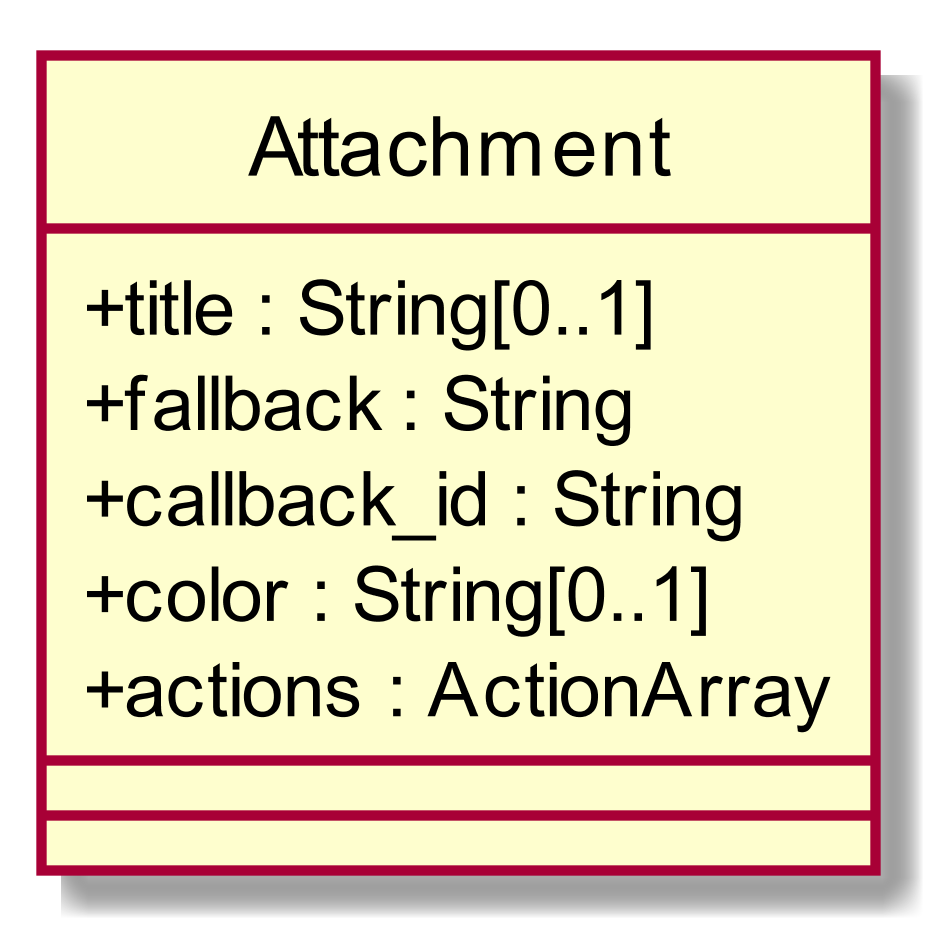
\includegraphics[width=0.35\textwidth,height=\textheight,keepaspectratio]{images/ClassAttachment.png}
	\caption{Back-end::Notifications::Attachment}
\end{figure}
\begin{itemize}
	\item \textbf{Nome}: \file{Attachment};
	\item \textbf{Tipo}: \file{Class};
	\item \textbf{Descrizione}: questa classe si occupa di rappresentare e organizzare i dati relativi ad un \file{Attachment}
	;
	\item \textbf{Utilizzo}: fornisce gli attributi degli \file{Attachment} che dovranno essere aggiunti ad un \\ \file{NotificationMessage}.
	Un \file{Attachment}, contenuto in un \file{NotificationsMessage}, permette di aggiungere del significato ad un \file{NotificationMessage} ed arricchirlo tramite immagini, colori ed altro.
	Per la relativa documentazione, consultare questa pagina \url{https://api.slack.com/docs/message-buttons}  (visitato in data 2017-03-21);
	\item \textbf{Attributi}:
	\begin{itemize}
		\item[] \file{+ title: String[0..1]} \\
		Attributo contenente il titolo dell'\file{Attachment};
		\item[] \file{+ fallback: String} \\
		Attributo contenente un messaggio mostrato agli utenti che utilizzano un'interfaccia che non supporta gli attachments;
		\item[] \file{+ callback\_id: String} \\
		Attributo contenente l'id della collezione di bottoni all'interno dell'\file{Attachment};
		\item[] \file{+ color: String[0..1]} \\
		Attributo contenente il colore dell'\file{Attachment};
		\item[] \file{+ actions: ActionArray} \\
		Attributo contenente una array di \file{Action} da includere nell'\file{Attachment}. Questo array può contenere al massimo cinque \file{Action};
	\end{itemize}
	\item \textbf{Relazioni con le altre classi}:
	\begin{itemize}
		\item IN \hyperlink{NotificationMessage_label}{\file{NotificationMessage}}
		\item OUT \hyperlink{Action_label}{\file{Action}}
	\end{itemize}
\end{itemize}
\FloatBarrier

\hypertarget{ConfirmationFields_label}{\subparagraph{ConfirmationFields}}
\begin{figure}[h]
	\centering
	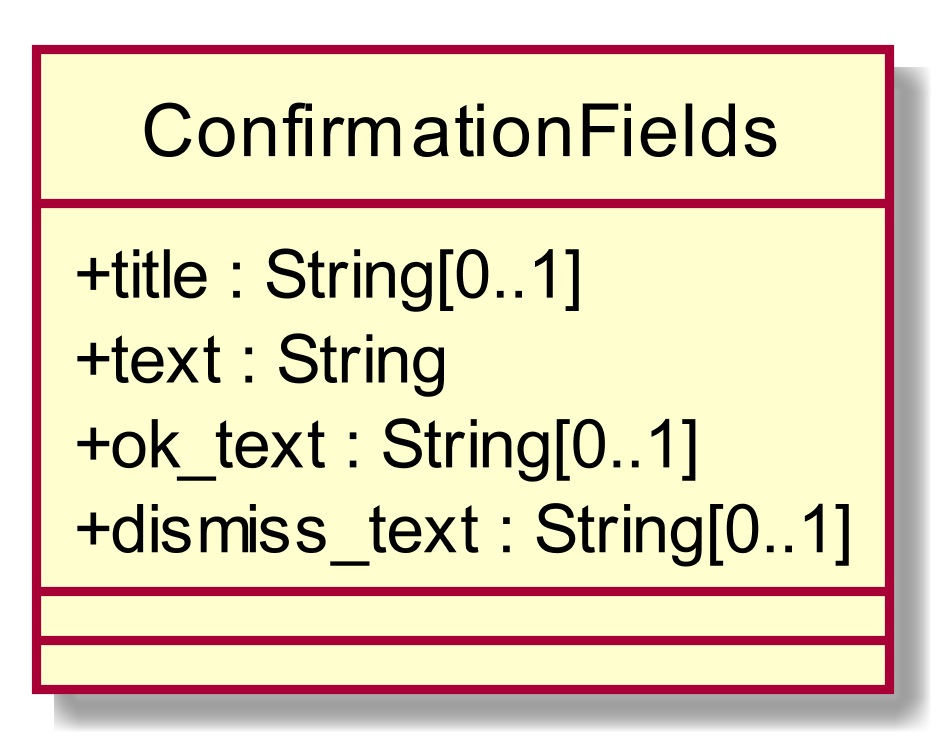
\includegraphics[width=0.35\textwidth,height=\textheight,keepaspectratio]{images/ClassConfirmationFields.png}
	\caption{Back-end::Notifications::ConfirmationFields}
\end{figure}
\begin{itemize}
	\item \textbf{Nome}: \file{ConfirmationFields};
	\item \textbf{Tipo}: \file{Class};
	\item \textbf{Descrizione}: questa classe si occupa di rappresentare e organizzare gli attributi relativi ad un messaggio di conferma di Slack;
	\item \textbf{Utilizzo}: fornisce gli attributi per rappresentare un messaggio di conferma di Slack.
	\\
	Per la relativa documentazione, consultare la pagina \url{https://api.slack.com/docs/message-buttons}  (visitato in data 2017-03-21);
	\item \textbf{Attributi}:
	\begin{itemize}
		\item[] \file{+ title: String[0..1]} \\
		Attributo contenente il titolo della finestra di pop up;
		\item[] \file{+ text: String} \\
		Attributo contenente la descrizione dettagliata delle conseguenze della relativa \file{Action} e contestualizza le scelte fornite dal button;
		\item[] \file{+ ok\_text: String[0..1]} \\
		Attributo contenente il testo del bottone che serve per confermare la relativa \file{Action}. Il valore di default per questo attributo è "Okay".
		;
		\item[] \file{+ dismiss\_text: String[0..1]} \\
		Attributo contenente il testo del bottone che serve per cancellare la relativa \file{Action}. Il valore di default per questo attributo è "Cancel";
	\end{itemize}
	\item \textbf{Relazioni con le altre classi}:
	\begin{itemize}
		\item IN \hyperlink{Action_label}{\file{Action}}
	\end{itemize}
\end{itemize}
\FloatBarrier

\hypertarget{NotificationChannel_label}{\subparagraph{NotificationChannel}}
\begin{figure}[h]
	\centering
	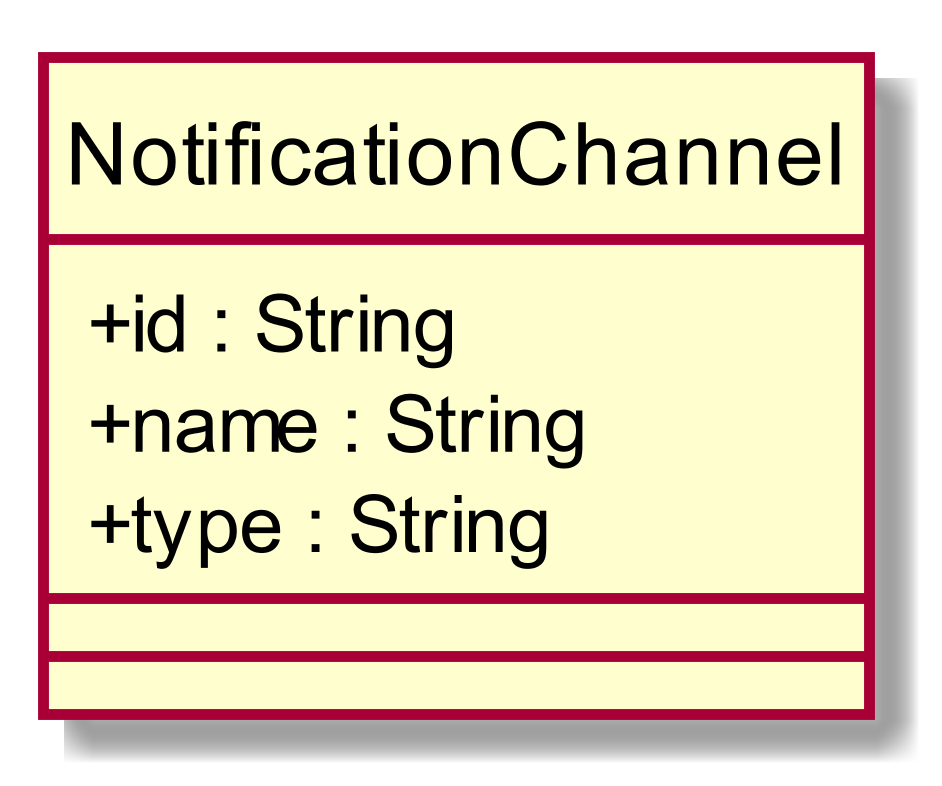
\includegraphics[width=0.35\textwidth,height=\textheight,keepaspectratio]{images/ClassNotificationChannel.png}
	\caption{Back-end::Notifications::NotificationChannel}
\end{figure}
\begin{itemize}
	\item \textbf{Nome}: \file{NotificationChannel};
	\item \textbf{Tipo}: \file{Class};
	\item \textbf{Descrizione}: questa classe si occupa di rappresentare e organizzare i parametri relativi al canale Slack nel quale spedire il \file{NotificationMessage};
	\item \textbf{Utilizzo}: fornisce gli attributi di un \file{NotificationChannel}. \\
	Per consultare la relativa documentazione, consultare questa pagina \url{https://api.slack.com/types/channel} (visitato in data 2017-03-21);
	\item \textbf{Attributi}:
	\begin{itemize}
		\item[] \file{+ id: String} \\
		Attributo contenente l'id del canale Slack;
		\item[] \file{+ name: String} \\
		Attributo contenente il nome del canale Slack;
		\item[] \file{+ type: String} \\
		Attributo che indica il tipo del canale. \\ Può assumere i seguenti valori:
		\begin{itemize}
			\item user: il canale rappresenta un utente Slack;
			\item channel: il canale rappresenta un canale pubblico Slack;
			\item group: il canale rappresenta un canale privato Slack.
		\end{itemize}
	\end{itemize}
	\item \textbf{Relazioni con le altre classi}:
	\begin{itemize}
		\item IN \hyperlink{NotificationService_label}{\file{NotificationService}}
	\end{itemize}
\end{itemize}
\FloatBarrier

\hypertarget{NotificationMessage_label}{\subparagraph{NotificationMessage}}
\begin{figure}[h]
	\centering
	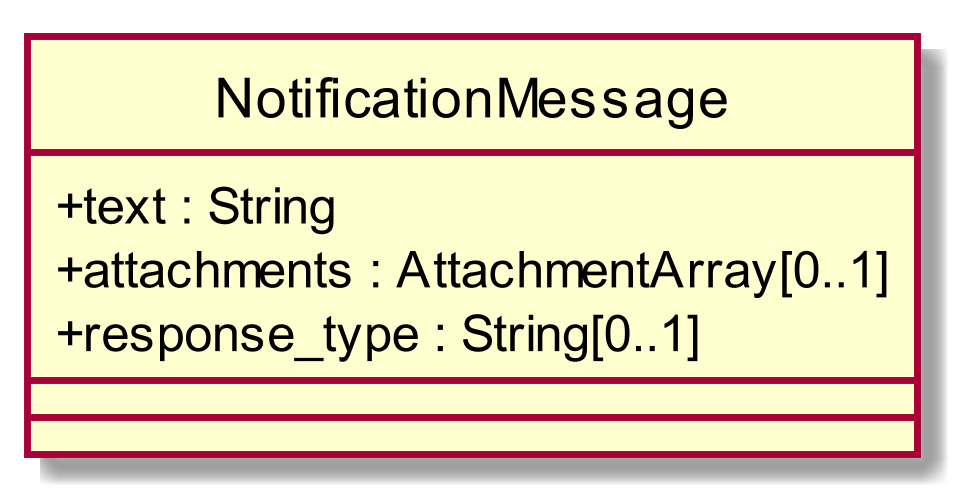
\includegraphics[width=0.35\textwidth,height=\textheight,keepaspectratio]{images/ClassNotificationMessage.png}
	\caption{Back-end::Notifications::NotificationMessage}
\end{figure}
\begin{itemize}
	\item \textbf{Nome}: \file{NotificationMessage};
	\item \textbf{Tipo}: \file{Class};
	\item \textbf{Descrizione}: questa classe si occupa di rappresentare e organizzare i parametri relativi al messaggio da spedire nel \file{NotificationChannel};
	\item \textbf{Utilizzo}: fornisce gli attributi di un \file{NotificationChannel}. \\ Per consultare la relativa documentazione, consultare questa pagina \url{https://api.slack.com/docs/message-formatting} (visitato in data 2017-03-21);
	\item \textbf{Attributi}:
	\begin{itemize}
		\item[] \file{+ text: String} \\
		Attributo contenente il testo del \file{NotificationMessage};
		\item[] \file{+ attachments: AttachmentArray[0..1]} \\
		Attributo contenente l'array degli attachments del \file{NotificationMessage};
		\item[] \file{+ response\_type: String[0..1]} \\
		Attributo contenente il modo con il quale notificare.
		Questo attributo può assumere uno tra i seguenti valori:
		\begin{itemize}
			\item \file{in\_channel}, che mostra il \file{NotificationMessage} ai membri del canale con il message button già cliccato;
			\item \file{ephemeral}, che mostra il \file{NotificationMessage} ai membri del canale che cliccano sul message button.
		\end{itemize}
		Per la relativa documentazione, consultare questa pagina \url{https://api.slack.com/docs/message-buttons}  (visitato in data 2017-03-21);
	\end{itemize}
	\item \textbf{Relazioni con le altre classi}:
	\begin{itemize}
		\item IN \hyperlink{NotificationService_label}{\file{NotificationService}}
		\item OUT \hyperlink{Attachment_label}{\file{Attachment}}
	\end{itemize}
\end{itemize}
\FloatBarrier

\hypertarget{NotificationService_label}{\subparagraph{NotificationService}}
\begin{figure}[h]
	\centering
	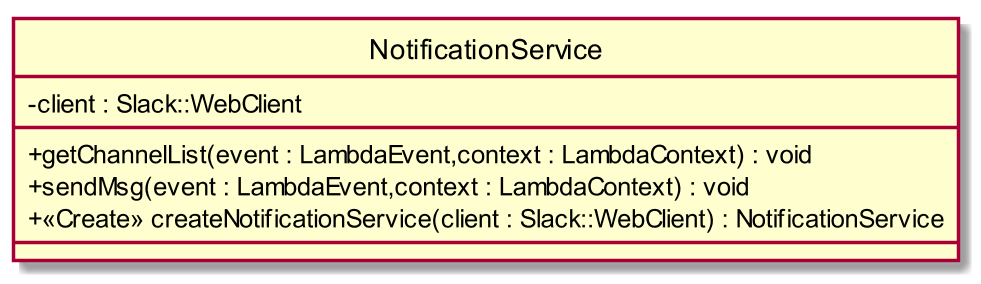
\includegraphics[width=0.65\textwidth,height=\textheight,keepaspectratio]{images/ClassNotificationService.png}
	\caption{Back-end::Notifications::NotificationService}
\end{figure}
\begin{itemize}
	\item \textbf{Nome}: \file{NotificationService};
	\item \textbf{Tipo}: \file{Class};
	\item \textbf{Descrizione}: questa classe si occupa di realizzare il microservizio \file{Notifications};
	\item \textbf{Utilizzo}: fornisce i metodi che implementano le Lambda Function necessarie per notificare la persona desiderata sul relativo canale Slack;
	\item \textbf{Attributi}:
	\begin{itemize}
		\item[] \file{- client: Slack::WebClient} \\
		Questo attributo è utilizzato per interagire con le API Web di Slack;
	\end{itemize}
	\item \textbf{Metodi}:
	\begin{itemize}
		\item[] \file{+ getChannelList(event: LambdaEvent, context: LambdaContext): void}\\ \\		Metodo che implementa la Lambda Function che si occupa di restituire l'array dei canali Slack disponibili. Si occupa di chiamare i metodi \file{users.list}, \file{channels.list} e \file{groups.list} delle API di Slack, quindi combina i risultati ottenuti da queste chiamate in un array di \file{NotificationChannel}, eliminando i dati in più;\\
		Parametri:
		\begin{itemize}
			\item \file{event: LambdaEvent} \\
			Parametro che rappresenta la richiesta ricevuta dal \file{VocalAPI}. Il campo \file{body} di questo attributo conterrà una stringa vuota;
			\item \file{context: LambdaContext} \\
			Parametro utilizzato dalle Lambda Function per inviare la risposta. Il \file{body} del \file{LambdaResponse}, parametro del metodo \file{LambdaContext::succeed}, conterrà un array di oggetti di tipo \file{NotificationChannel};
		\end{itemize}
		\item[] \file{+ sendMsg(event: LambdaEvent, context: LambdaContext): void} \\		Metodo che implementa la Lambda Function che si occupa di inviare il messaggio alla persona desiderata;\\
		Parametri:
		\begin{itemize}
			\item \file{event: LambdaEvent} \\
			Parametro contenente, all'interno del campo \file{body} sotto forma di stringa in formato JSON, un oggetto contenente tutti i dati relativi ad un messaggio da inviare.
			Tali dati sono:
			\begin{lstlisting}[language=json,firstnumber=1]
			{
			"msg":"NotificationMessage",
			"send_to":"String"
			}
			\end{lstlisting}
			Dove \file{msg} è un oggetto di tipo \file{NotificationMessage}, mentre \file{send\_to} è una stringa contenente il mittente del messaggio;
			\item \file{context: LambdaContext} \\
			Parametro utilizzato dalle Lambda Function per inviare la risposta. La risposta, contenuta nel \file{LambdaResponse} parametro del metodo \file{LambdaContext::succeed}, possiede un attributo \file{body}, il quale conterrà una stringa vuota. Il risultato delle operazioni di questo metodo sarà deducibile tramite il valore dell'attributo \\ \file{LambaResponse::statusCode};
		\end{itemize}
		\item[] \file{+ <<Create>> createNotificationService(client: Slack::WebClient):\\ NotificationService} \\		Costruttore, si occupa di gestire la dependency injection di \file{Slack::WebClient};\\
		Parametri:
		\begin{itemize}
			\item \file{client: Slack::WebClient} \\
			Parametro contenente l'istanza di \file{Slack::WebClient} di cui viene effettuata la dependency injection;
		\end{itemize}
	\end{itemize}
	\item \textbf{Relazioni con le altre classi}:
	\begin{itemize}
		\item OUT \hyperlink{LambdaContext_label}{\file{LambdaContext}}
		\item OUT \hyperlink{LambdaEvent_label}{\file{LambdaEvent}}
		\item OUT \hyperlink{NotificationChannel_label}{\file{NotificationChannel}}
		\item OUT \hyperlink{NotificationMessage_label}{\file{NotificationMessage}}
	\end{itemize}
\end{itemize}
\FloatBarrier

\newpage \subsubsection{Back-end::Rules}
Package contenente le classi e le interfacce che realizzano il microservizio di gestione delle direttive per l'assistente virtuale.\\
Vengono offerte funzionalità che permettono:
\begin{itemize}
	\item l'aggiunta di una nuova direttiva;
	\item l'aggiunta di un nuovo compito (\file{Task}) che una direttiva deve eseguire;
	\item la gestione delle direttive esistenti;
	\item la gestione dei compiti esistenti.
\end{itemize}
\begin{figure}[h] \centering 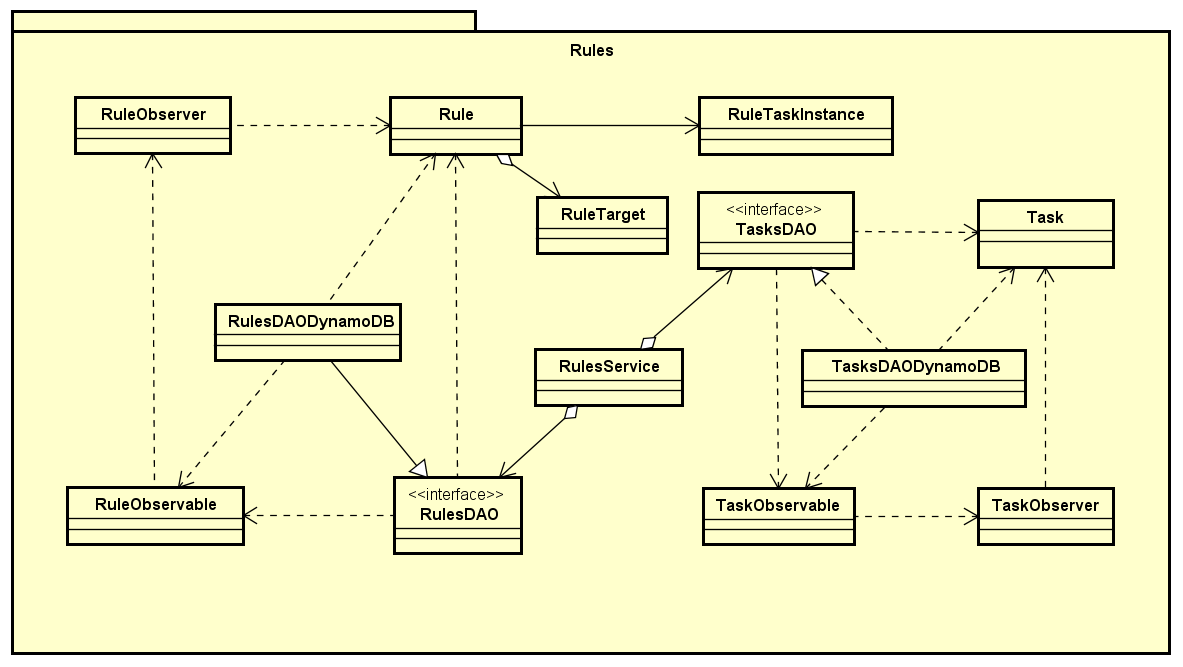
\includegraphics[width=\textwidth,height=\textheight,keepaspectratio]{images/diagrams/back-end/Official_Backend_0304/Rules.png}
	\caption{Package Back-end::Rules}
\end{figure}
\newpage

\paragraph{Classi}
\hypertarget{ RulesDAO_label}{\subparagraph{ RulesDAO}}
\begin{figure}[h]
	\centering
	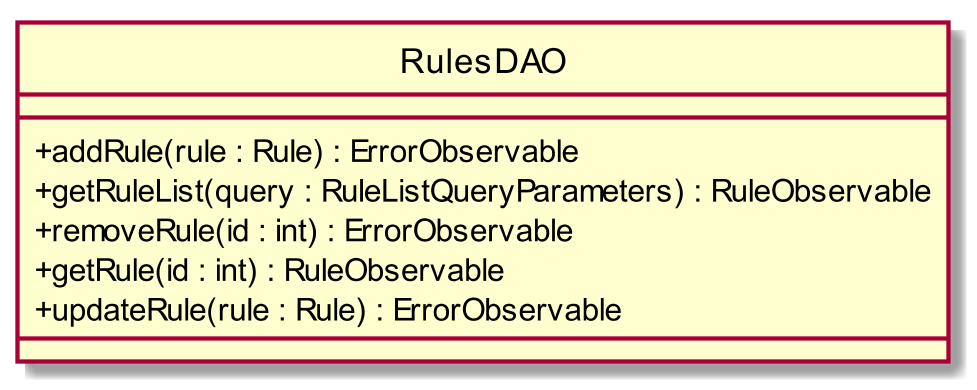
\includegraphics[width=0.65\textwidth,height=\textheight,keepaspectratio]{images/ClassRulesDAO.png}
	\caption{Back-end::Rules:: RulesDAO}
\end{figure}
\begin{itemize}
	\item \textbf{Nome}: \file{ RulesDAO};
	\item \textbf{Tipo}: \file{Interface};
	\item \textbf{Descrizione}: questa classe si occupa di astrarre le modalità di accesso al database per questo microservizio, contenente le \file{Rule};
	\item \textbf{Utilizzo}: fornisce a \file{RuleService} un meccanismo per accedere al database, contenente le \file{Rule}, senza conoscerne le modalità di implementazioni e di persistenza del database. A partire da un identificativo, permette operazioni di lettura, scrittura e rimozione delle \file{Rule};
	\item \textbf{Figlio}: \file{RulesDAODynamoDB};
	\item \textbf{Metodi}:
	\begin{itemize}
		\item[] \file{+ addRule(rule: Rule): ErrorObservable} \\		Metodo che permette di aggiungere una \file{Rule} al database. L'\file{Observable} restituito non riceverà alcun valore, ma verrà completato in caso di aggiunta della \file{Rule} avvenuta con successo. In caso di errore durante l'aggiunta della \file{Rule}, gli \file{Observer} interessati verranno notificati tramite la chiamata del loro metodo \file{error} con i dati relativi all'errore verificatosi;\\
		Parametri:
		\begin{itemize}
			\item \file{rule: Rule} \\
			Parametro contenente la \file{Rule} da aggiungere;
		\end{itemize}
		\item[] \file{+ getRulesList(): RuleObservable} \\		L'\file{Observable} restituito manderà agli \file{Observer} le direttive ottenute, una alla volta, e poi chiama il loro metodo \file{complete}. Nel caso in cui si verifichi un errore, gli \file{Observer} iscritti verranno notificati tramite la chiamate del loro metodo \file{error} con i dati relativi all'errore verificatosi;\\
		\item[] \file{+ removeRule(id: int): ErrorObservable} \\		Metodo che permette di rimuovere una \file{Rule} dal database. L'\file{Observable} restituito non riceverà alcun valore, ma verrà completato in caso di rimozione della \file{Rule} avvenuta con successo. In caso di errore durante la rimozione della \file{Rule}, gli \file{Observer} interessati verranno notificati tramite la chiamata del loro metodo \file{error} con i dati relativi all'errore verificatosi;\\
		Parametri:
		\begin{itemize}
			\item \file{id: int} \\
			Parametro contenente l'id della \file{Rule};
		\end{itemize}
		\item[] \file{+ getRule(id: int): RuleObservable} \\		Metodo che permette di ottenere una \file{Rule} a partire dal suo Id. L'\file{Observable} restituito riceverà l'oggetto rappresentante tale \file{Rule}, e verrà completato. Nel caso in cui la \file{Rule} richiesta non sia presente nel database, gli \file{Observer} interessati non riceveranno alcun valore, ma verranno notificati tramite la chiamata del loro metodo \file{error};\\
		Parametri:
		\begin{itemize}
			\item \file{id: int} \\
			Parametro contenente l'id della \file{Rule} da recuperare;
		\end{itemize}
		\item[] \file{+ updateRule(rule: Rule): ErrorObservable} \\		Metodo che permette di aggiornare una \file{Rule}. L'\file{Observable} restituito non riceverà alcun valore, ma verrà completato in caso di aggiornamento della \file{Rule} avvenuta con successo. In caso di errore durante l'aggiornamento della \file{Rule}, gli \file{Observer} interessati verranno notificati tramite la chiamata del loro metodo \file{error} con i dati relativi all'errore verificatosi;\\
		Parametri:
		\begin{itemize}
			\item \file{rule: Rule} \\
			Parametro contenente la \file{Rule};
		\end{itemize}
		\item[] \file{+ query(target: RuleTarget, type: StringArray = null): RuleArray}\\ \\		Metodo che permette di interrogare il DAO e richiedere la lista delle direttive che si applicano ad un determinato target;\\
		Parametri:
		\begin{itemize}
			\item \file{target: RuleTarget} \\
			Parametro contenente il target del quale si vogliono ottenere le direttive;
			\item \file{type: StringArray = null} \\
			Parametro contenente la lista dei tipi di \gl{task} che devono essere tenuti in considerazione. Se impostato a null, verranno tenuti in considerazione tutti i tipi di task;
		\end{itemize}
	\end{itemize}
	\item \textbf{Relazioni con le altre classi}:
	\begin{itemize}
		\item IN \hyperlink{AdministrationWebhookService_label}{\file{AdministrationWebhookService}}
		\item IN \hyperlink{RulesService_label}{\file{RulesService}}
		\item OUT \hyperlink{Rule_label}{\file{Rule}}
		\item OUT \hyperlink{RuleObservable_label}{\file{RuleObservable}}
		\item OUT \hyperlink{ErrorObservable_label}{\file{ErrorObservable}}
	\end{itemize}
\end{itemize}
\FloatBarrier

\hypertarget{ TasksDAO_label}{\subparagraph{ TasksDAO}}
\begin{figure}[h]
	\centering
	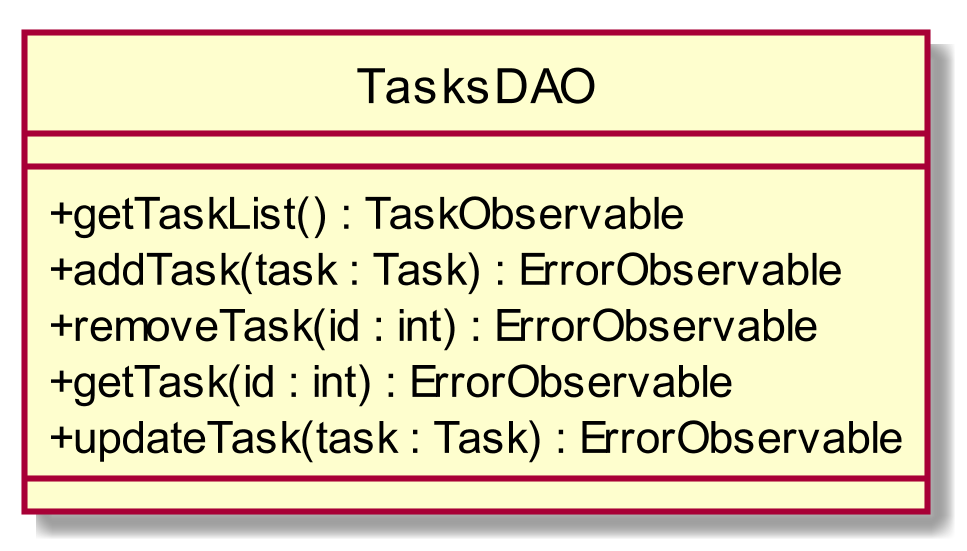
\includegraphics[width=0.50\textwidth,height=\textheight,keepaspectratio]{images/ClassTasksDAO.png}
	\caption{Back-end::Rules:: TasksDAO}
\end{figure}
\begin{itemize}
	\item \textbf{Nome}: \file{ TasksDAO};
	\item \textbf{Tipo}: \file{Interface};
	\item \textbf{Descrizione}: questa classe si occupa di astrarre le modalità d'accesso al database per questo microservizio, contenente i \file{Task};
	\item \textbf{Utilizzo}: fornisce a \file{RuleService} un meccanismo per accedere al database, contenente i compiti da applicare a certe \file{Rule}, senza conoscerne le modalità di implementazioni e di persistenza del database. A partire da un identificativo, permette operazioni di lettura, scrittura e rimozione dei \file{Task};
	\item \textbf{Figlio}: \file{TasksDAODynamoDB};
	\item \textbf{Metodi}:
	\begin{itemize}
		\item[] \file{+ getTaskList(): TaskObservable} \\		Metodo che permette di ottenere la lista dei compiti. L'\file{Observable} restituito manderà agli \file{Observer} i compiti ottenuti, una alla volta, e poi chiama il loro metodo \file{complete}. Nel caso in cui si verifichi un errore, gli \file{Observer} iscritti verranno notificati tramite la chiamate del loro metodo \file{error} con i dati relativi all'errore verificatosi;\\
		\item[] \file{+ addTask(task: Task): ErrorObservable} \\		Metodo che permette di aggiungere un \file{Task} al database. \\ L'\file{Observable} restituito non riceverà alcun valore, ma verrà completato in caso di aggiunta del \file{Task} avvenuta con successo. In caso di errore durante l'aggiunta del \file{Task}, gli \file{Observer} interessati verranno notificati tramite la chiamata del loro metodo \file{error} con i dati relativi all'errore verificatosi;\\
		Parametri:
		\begin{itemize}
			\item \file{task: Task} \\
			Parametro contenente il compito;
		\end{itemize}
		\item[] \file{+ removeTask(id: int): ErrorObservable} \\		Metodo che permette di rimuovere un compito dal database a partire dal suo id. \\ L'\file{Observable} restituito non riceverà alcun valore, ma verrà completato in caso di rimozione del \file{Task} avvenuta con successo. In caso di errore durante la rimozione del \file{Task}, gli \file{Observer} interessati verranno notificati tramite la chiamata del loro metodo \file{error} con i dati relativi all'errore verificatosi;\\
		Parametri:
		\begin{itemize}
			\item \file{id: int} \\
			Parametro contenente l'id della funzione;
		\end{itemize}
		\item[] \file{+ getTask(id: int): ErrorObservable} \\		Metodo che permette di ottenere un \file{Task} a partire dal suo id. \\ L'\file{Observable} restituito riceverà l'oggetto rappresentante tale \file{Task}, e verrà completato. Nel caso in cui il \file{Task} richiesto non sia presente nel database, gli \file{Observer} interessati non riceveranno alcun valore, ma verranno notificati tramite la chiamata del loro metodo \file{error};\\
		Parametri:
		\begin{itemize}
			\item \file{id: int} \\
			Parametro contenente l'id della funzione;
		\end{itemize}
		\item[] \file{+ updateTask(task: Task): ErrorObservable} \\		Metodo che permette di aggiornare un compito. L'\file{Observable} restituito non riceverà alcun valore, ma verrà completato in caso di aggiunta del \file{Task} con successo. In caso di errore durante l'aggiunta del \file{Task}, gli \file{Observer} interessati verranno notificati tramite la chiamata del loro metodo \file{error} con i dati relativi all'errore verificatosi;\\
		Parametri:
		\begin{itemize}
			\item \file{task: Task} \\
			Parametro contenente il compito;
		\end{itemize}
	\end{itemize}
	\item \textbf{Relazioni con le altre classi}:
	\begin{itemize}
		\item IN \hyperlink{RulesService_label}{\file{RulesService}}
		\item OUT \hyperlink{Task_label}{\file{Task}}
		\item OUT \hyperlink{TaskObservable_label}{\file{TaskObservable}}
		\item OUT \hyperlink{ErrorObservable_label}{\file{ErrorObservable}}
	\end{itemize}
\end{itemize}
\FloatBarrier

\hypertarget{Rule_label}{\subparagraph{Rule}}
\begin{figure}[h]
	\centering
	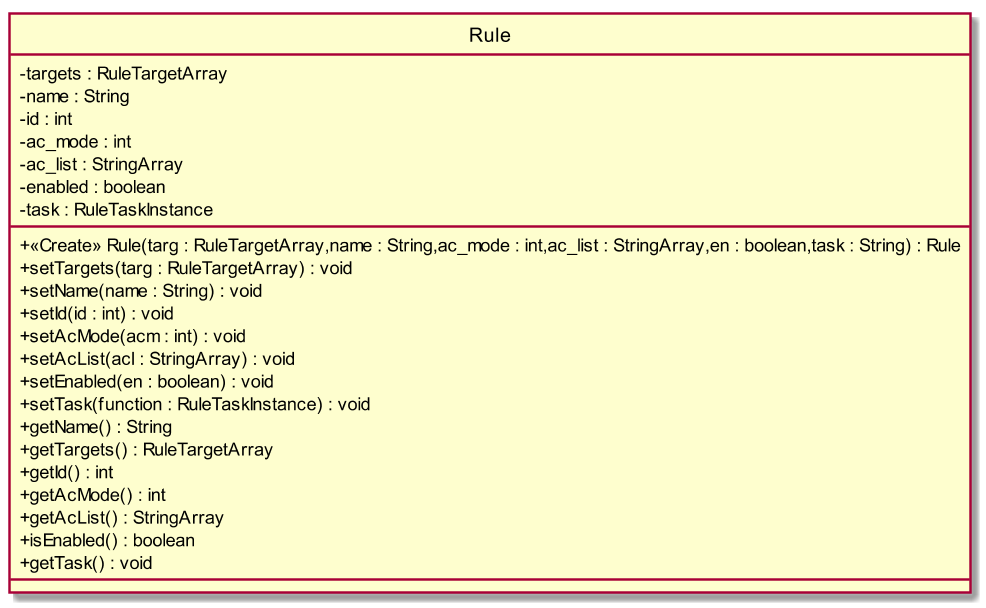
\includegraphics[width=0.90\textwidth,height=\textheight,keepaspectratio]{images/ClassRule.png}
	\caption{Back-end::Rules::Rule}
\end{figure}
\begin{itemize}
	\item \textbf{Nome}: \file{Rule};
	\item \textbf{Tipo}: \file{Class};
	\item \textbf{Descrizione}: questa classe si occupa di rappresentare e organizzare i dati relativi ad una \file{Rule}, ovvero una direttiva definita da un amministratore;
	\item \textbf{Utilizzo}: fornisce i metodi getter e setter per i parametri relativi ad una direttiva, i quali dovranno essere memorizzati nel database per questo microservizio. Tramite il metodo \file{setTask}, è soggetta ad una setter-based dependency injection che ha come oggetto una \file{RuleTaskInstance}. \\
	È utilizzata dalla classe \file{RulesDAO} e dalle classi che utilizzano quest'ultima;
	\item \textbf{Attributi}:
	\begin{itemize}
		\item[] \file{- targets: RuleTargetArray} \\
		Attributo contenente i targets della \file{Rule};
		\item[] \file{- name: String} \\
		Attributo contenente il nome della \file{Rule};
		\item[] \file{- id: int} \\
		Attributo contenente l'id della \file{Rule};
		\item[] \file{- enabled: boolean} \\
		Attributo contenente un valore che dice se la \file{Rule} è abilitata o meno;
		\item[] \file{- task: RuleTaskInstance} \\
		Attributo contenente il compito della \file{Rule};
	\end{itemize}
	\item \textbf{Metodi}:
	\begin{itemize}
		\item[] \file{+ <<Create>> Rule(targ: RuleTargetArray, name: String, en: boolean, task: String): Rule} \\		Metodo che permette di instanziare un oggetto \file{Rule} a partire da un nome, una lista dei targets, un compito da applicare e un valore booleano per abilitarla o meno;\\
		Parametri:
		\begin{itemize}
			\item \file{targ: RuleTargetArray} \\
			Parametro contenente l'array dei targets da assegnare alla \file{Rule};
			\item \file{name: String} \\
			Parametro contenente il nome da assegnare alla \file{Rule};
			\item \file{en: boolean} \\
			Parametro contenente il valore booleano da assegnare alla \file{Rule} per abilitarla o meno;
			\item \file{task: String} \\
			Parametro contenente il compito da assegnare alla \file{Rule};
		\end{itemize}
		\item[] \file{+ setTargets(targ: RuleTargetArray): void} \\		Metodo che permette di passare un Array contenente i targets per la \file{Rule};\\
		Parametri:
		\begin{itemize}
			\item \file{targ: RuleTargetArray} \\
			Parametro contenente l'array dei targets da passare;
		\end{itemize}
		\item[] \file{+ setName(name: String): void} \\		Metodo che permette di modificare il nome della \file{Rule};\\
		Parametri:
		\begin{itemize}
			\item \file{name: String} \\
			Parametro contenente il nome della Rule da passare;
		\end{itemize}
		\item[] \file{+ setId(id: int): void} \\		Metodo che permette di modificare l'id della \file{Rule};\\
		Parametri:
		\begin{itemize}
			\item \file{id: int} \\
			Parametro contenente l'id da passare;
		\end{itemize}
		\item[] \file{+ setEnabled(en: boolean): void} \\		Metodo che permette di passare un valore da impostare ad \file{enabled} per la \file{Rule};\\
		Parametri:
		\begin{itemize}
			\item \file{en: boolean} \\
			Parametro contenente il valore booleano da passare;
		\end{itemize}
		\item[] \file{+ setTask(function: RuleTaskInstance): void} \\		Metodo che permette di modificare il compito da applicare alla \file{Rule};\\
		Parametri:
		\begin{itemize}
			\item \file{function: RuleTaskInstance} \\
			Parametro contenente la function da passare;
		\end{itemize}
		\item[] \file{+ getName(): String} \\		Metodo che permette di ottenere il nome della \file{Rule};\\
		\item[] \file{+ getTargets(): RuleTargetArray} \\		Metodo che permette di ottenere l'array contenente i targets della \file{Rule};\\
		\item[] \file{+ getId(): int} \\		Metodo che permette di ottenere l'id della \file{Rule};\\
		\item[] \file{+ isEnabled(): boolean} \\		Metodo che permette di capire se la \file{Rule} è abilitata o meno;\\
		\item[] \file{+ getTask(): void} \\		Metodo che permette di ottenere il \file{Task} applicata dalla \file{Rule};\\
	\end{itemize}
	\item \textbf{Relazioni con le altre classi}:
	\begin{itemize}
		\item IN \hyperlink{<<interface>> RulesDAO_label}{\file{<<interface>> RulesDAO}}
		\item IN \hyperlink{RuleObserver_label}{\file{RuleObserver}}
		\item IN \hyperlink{RulesDAODynamoDB_label}{\file{RulesDAODynamoDB}}
		\item IN \hyperlink{VocalAPI_label}{\file{VocalAPI}}
		\item OUT \hyperlink{RuleTarget_label}{\file{RuleTarget}}
		\item OUT \hyperlink{RuleTaskInstance_label}{\file{RuleTaskInstance}}
	\end{itemize}
\end{itemize}
\FloatBarrier

\hypertarget{RuleObservable_label}{\subparagraph{RuleObservable}}
\begin{figure}[h]
	\centering
	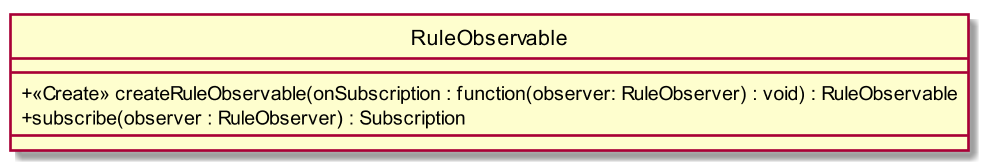
\includegraphics[width=\textwidth,height=\textheight,keepaspectratio]{images/ClassRuleObservable.png}
	\caption{Back-end::Rules::RuleObservable}
\end{figure}
\begin{itemize}
	\item \textbf{Nome}: \file{RuleObservable};
	\item \textbf{Tipo}: \file{Class};
	\item \textbf{Descrizione}: questa classe implementa un \file{Observable} che permette l'iscrizione di \file{RuleObserver};
	\item \textbf{Utilizzo}: fornisce i meccanismi necessari per il passaggio di una serie di \file{Rule} ad un \file{Observer} interessato;
	\item \textbf{Padre}: \file{Observable};
	\item \textbf{Metodi}:
	\begin{itemize}
		\item[] \file{+ <<Create>> createRuleObservable(onSubscription: function(observer\\: RuleObserver) : void): RuleObservable} \\		Constructor di \file{RuleObservable};\\
		Parametri:
		\begin{itemize}
			\item \file{onSubscription: function(observer: RuleObserver) : void} \\
			Funzione che verrà eseguita quando un \file{Observer} si iscrive all'\file{Observable}. Si occupa di passare i dati all'\file{Observer}, chiamando il metodo \file{next(rule: Rule)}. Quando non ci sono più dati da restituire, si occupa di chiamare il metodo \file{complete}. Nel caso in cui si verificasse un errore, si occupa di chiamare il metodo \file{error(err: Object)} con i dati relativi all'errore verificatosi;
		\end{itemize}
		\item[] \file{+ subscribe(observer: RuleObserver): Subscription} \\		Metodo che permette ad un \file{RuleObserver} interessato di iscriversi a questo \file{Observable};\\
		Parametri:
		\begin{itemize}
			\item \file{observer: RuleObserver} \\
			\file{Observer} che si vuole iscrivere;
		\end{itemize}
	\end{itemize}
	\item \textbf{Relazioni con le altre classi}:
	\begin{itemize}
		\item IN \hyperlink{RulesDAODynamoDB_label}{\file{RulesDAODynamoDB}}
		\item IN \hyperlink{<<interface>> RulesDAO_label}{\file{<<interface>> RulesDAO}}
		\item OUT \hyperlink{RuleObserver_label}{\file{RuleObserver}}
	\end{itemize}
\end{itemize}
\FloatBarrier

\hypertarget{RuleObserver_label}{\subparagraph{RuleObserver}}
\begin{figure}[h]
	\centering
	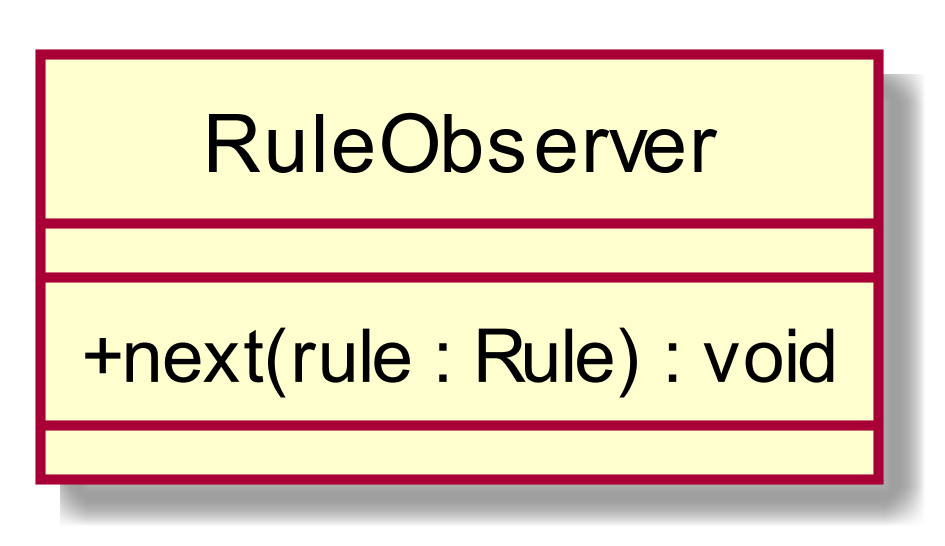
\includegraphics[width=0.35\textwidth,height=\textheight,keepaspectratio]{images/ClassRuleObserver.png}
	\caption{Back-end::Rules::RuleObserver}
\end{figure}
\begin{itemize}
	\item \textbf{Nome}: \file{RuleObserver};
	\item \textbf{Tipo}: \file{Class};
	\item \textbf{Descrizione}: classe che rappresenta un \file{Observer} che si aspetta dati di tipo \file{Rule};
	\item \textbf{Utilizzo}: ridefinisce il metodo \file{next} della classe ObserverAdapter, in maniera tale che accetti dati di tipo \file{Rule};
	\item \textbf{Metodi}:
	\begin{itemize}
		\item[] \file{+ next(rule: Rule): void} \\		Metodo che permette agli \file{Observable} di notificare l'\file{Observer} con dati di tipo \file{Rule}. Definisce inoltre le operazioni che l'\file{Observer} compierà all'arrivo di tali dati;\\
		Parametri:
		\begin{itemize}
			\item \file{rule: Rule} \\
			Parametro contenente la \file{Rule} mandata dall'\file{Observable};
		\end{itemize}
	\end{itemize}
	\item \textbf{Relazioni con le altre classi}:
	\begin{itemize}
		\item IN \hyperlink{RuleObservable_label}{\file{RuleObservable}}
		\item OUT \hyperlink{Rule_label}{\file{Rule}}
	\end{itemize}
\end{itemize}
\FloatBarrier

\hypertarget{RulesDAODynamoDB_label}{\subparagraph{RulesDAODynamoDB}}
\begin{figure}[h]
	\centering
	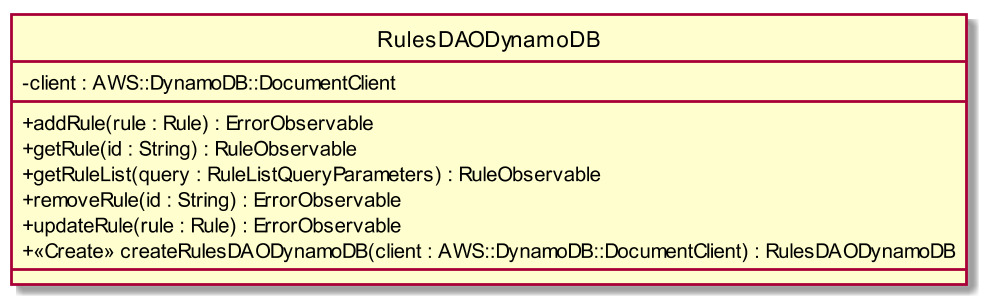
\includegraphics[width=0.60\textwidth,height=\textheight,keepaspectratio]{images/ClassRulesDAODynamoDB.png}
	\caption{Back-end::Rules::RulesDAODynamoDB}
\end{figure}
\begin{itemize}
	\item \textbf{Nome}: \file{RulesDAODynamoDB};
	\item \textbf{Tipo}: \file{Class};
	\item \textbf{Descrizione}: classe che si occupa di implementare l'interfaccia \file{RulesDAO}, utilizzando un database DynamoDB come supporto per la memorizzazione dei dati;
	\item \textbf{Utilizzo}: implementa i metodi dell'interfaccia \file{RulesDAO} interrogando un database DynamoDB. Utilizza \file{AWS::DynamoDB::DocumentClient} per l'accesso al database. La dependency injection dell'oggetto \file{AWS::DynamoDB} viene fatta utilizzando il costruttore;
	\item \textbf{Padre}: \file{<<interface>> RulesDAO};
	\item \textbf{Attributi}:
	\begin{itemize}
		\item[] \file{- client: AWS::DynamoDB::DocumentClient} \\
		Attributo contenente un riferimento al modulo di Node.js utilizzato per l'accesso al database DynamoDB contenente la tabella delle direttive;
	\end{itemize}
	\item \textbf{Metodi}:
	\begin{itemize}
		\item[] \file{+ addRule(rule: Rule): ErrorObservable} \\		Implementazione del metodo definito nell'interfaccia \file{RulesDAO}. Utilizza il metodo put del \file{DocumentClient} per aggiungere la Rule al database;\\
		Parametri:
		\begin{itemize}
			\item \file{rule: Rule} \\
			Parametro contenente la \file{Rule} da aggiungere;
		\end{itemize}
		\item[] \file{+ getRule(id: String): RuleObservable} \\		Implementazione del metodo definito nell'interfaccia \file{RulesDAO}. Utilizza il metodo get del \file{DocumentClient} per ottenere i dati relativi ad uno \file{Rule} dal database;\\
		Parametri:
		\begin{itemize}
			\item \file{id: String} \\
			Parametro contenente l'id della \file{Rule} da recuperare;
		\end{itemize}
		\item[] \file{+ getRuleList(): RuleObservable} \\		Implementazione del metodo dell'interfaccia \file{RulesDAO}. Utilizza il metodo scan del \file{DocumentClient} per ottenere la lista delle Rule dal database;\\
		\item[] \file{+ removeRule(id: String): ErrorObservable} \\		Implementazione del metodo dell'interfaccia \file{RulesDAO}. Utilizza il metodo delete del \file{DocumentClient} per eliminare una Rule dal database;\\
		Parametri:
		\begin{itemize}
			\item \file{id: String} \\
			Parametro contenente l'id della \file{Rule};
		\end{itemize}
		\item[] \file{+ updateRule(rule: Rule): ErrorObservable} \\		Implementazione del metodo dell'interfaccia \file{RulesDAO}. Utilizza il metodo update del \file{DocumentClient} per aggiornare i dati relativi ad una Rule presente all'interno del database;\\
		Parametri:
		\begin{itemize}
			\item \file{rule: Rule} \\
			Parametro contenente la \file{Rule} da aggiornare;
		\end{itemize}
		\item[] \file{+ <<Create>> createRulesDAODynamoDB(client: AWS::DynamoDB::DocumentClient)\\: RulesDAODynamoDB} \\		Constructor della classe \file{RulesDAODynamoDB}. Permette di effettuare la dependency injection di \file{AWS::DynamoDB};\\
		Parametri:
		\begin{itemize}
			\item \file{client: AWS::DynamoDB::DocumentClient} \\
			Parametro contenente un riferimento al modulo di Node.js da utilizzare per l'accesso al database DynamoDB contenente la tabella delle rule;
		\end{itemize}
	\end{itemize}
	\item \textbf{Relazioni con le altre classi}:
	\begin{itemize}
		\item OUT \hyperlink{Rule_label}{\file{Rule}}
		\item OUT \hyperlink{RuleObservable_label}{\file{RuleObservable}}
		\item OUT \hyperlink{ErrorObservable_label}{\file{ErrorObservable}}
	\end{itemize}
\end{itemize}
\FloatBarrier

\hypertarget{RulesService_label}{\subparagraph{RulesService}}
\begin{figure}[h]
	\centering
	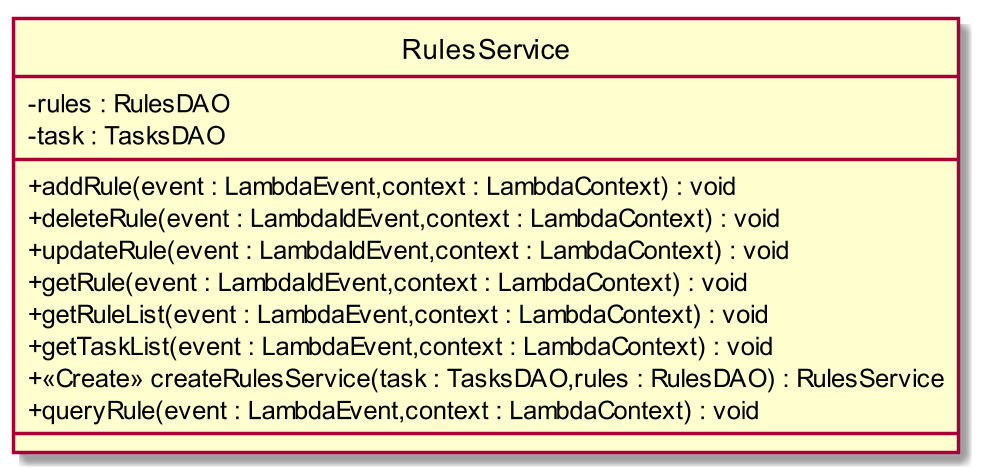
\includegraphics[width=0.80\textwidth,height=\textheight,keepaspectratio]{images/ClassRulesService.png}
	\caption{Back-end::Rules::RulesService}
\end{figure}
\begin{itemize}
	\item \textbf{Nome}: \file{RulesService};
	\item \textbf{Tipo}: \file{Class};
	\item \textbf{Descrizione}: questa classe si occupa di realizzare il microservizio \file{Rules} e di interagire con il database delle direttive;
	\item \textbf{Utilizzo}: fornisce i metodi che implementano le Lambda Function necessarie alla gestione delle \file{Rule} e relative \file{Task}. Questa classe non interagisce direttamente con il database, ma fa utilizzo di \file{TasksDAO} e \file{RulesDAO}, le quali nascondono i meccanismi di accesso e persistenza dei dati nel database;
	\item \textbf{Attributi}:
	\begin{itemize}
		\item[] \file{- rules: RulesDAO} \\
		Attributo che permette di contattare il \file{RulesDAO}, il quale permette l'accesso al database delle \file{Rule};
		\item[] \file{- task: TasksDAO} \\
		Attributo che permette di contattare il \file{TasksDAO}, il quale permette di accedere al database delle \file{Task};
	\end{itemize}
	\item \textbf{Metodi}:
	\begin{itemize}
		\item[] \file{+ addRule(event: LambdaEvent, context: LambdaContext): void} \\		Metodo che implementa la Lambda Function che si occupa di aggiungere una \file{Rule};\\
		Parametri:
		\begin{itemize}
			\item \file{event: LambdaEvent} \\
			Parametro contenente, all'interno del campo body sotto forma di stringa in formato JSON, un oggetto \file{Rule} contenente tutti i dati relativi ad una Rule da inserire;
			\item \file{context: LambdaContext} \\
			Parametro utilizzato dalle Lambda Function per inviare la risposta. Il \file{body} del \file{LambdaResponse}, parametro del metodo \file{LambdaContext::succeed}, conterrà una stringa vuota e il risultato di questa operazione sarà deducibile dal valore dell'attributo di \file{LambdaResponse::statusCode};
		\end{itemize}
		\item[] \file{+ deleteRule(event: LambdaIdEvent, context: LambdaContext): void}\\ \\		Metodo che implementa la Lambda Function che si occupa di eliminare una \file{Rule};\\
		Parametri:
		\begin{itemize}
			\item \file{event: LambdaIdEvent} \\
			Parametro contenente, all'interno del campo \file{pathParameters}, l'identificativo della \file{Rule} che si vuole eliminare;
			\item \file{context: LambdaContext} \\
			Parametro utilizzato dalle Lambda Function per inviare la risposta. Il \file{body} del \file{LambdaResponse}, ottenuto dal metodo \file{LambdaContext::succeed}, conterrà una stringa vuota e il risultato di questa operazione sarà deducibile dal valore dell'attributo \file{LambdaResponse::statusCode};
		\end{itemize}
		\item[] \file{+ updateRule(event: LambdaIdEvent, context: LambdaContext): void}\\ \\		Metodo che implementa la Lambda Function che si occupa di aggiornare una \file{Rule};\\
		Parametri:
		\begin{itemize}
			\item \file{event: LambdaIdEvent} \\
			Parametro contenente all'interno del campo \file{body}, sotto forma di stringa in formato JSON, un oggetto di tipo \file{Rule} contente i dati da aggiornare e, all'interno del campo \file{pathParameters}, l'identificativo della \file{Rule} da modificare;
			\item \file{context: LambdaContext} \\
			Parametro utilizzato dalle Lambda Function per inviare la risposta. Il \file{body} del \file{LambdaResponse}, ottenuto dal metodo \file{LambdaContext::succeed}, conterrà una stringa vuota e il risultato di questa operazione sarà deducibile dal valore dell'attributo \file{LambaResponse::statusCode};
		\end{itemize}
		\item[] \file{+ getRule(event: LambdaIdEvent, context: LambdaContext): void} \\\\		Metodo che implementa la Lambda Function che si occupa di ottenere una \file{Rule};\\
		Parametri:
		\begin{itemize}
			\item \file{event: LambdaIdEvent} \\
			Parametro contenente, all'interno del campo pathParameters, l'identificativo della \file{Rule} della quale si vogliono ottenere i dati;
			\item \file{context: LambdaContext} \\
			Parametro utilizzato dalle Lambda Function per inviare la risposta. Il \file{body} del \file{LambdaResponse}, ottenuto dal metodo \file{LambdaContext::succeed}, conterrà, sotto forma di stringa in formato JSON, un oggetto di tipo \file{Rule}, contenente i dati relativi alla \file{Rule} ritornata;
		\end{itemize}
		\item[] \file{+ getRuleList(event: LambdaEvent, context: LambdaContext): void} \\\\		Metodo che implementa la Lambda Function che si occupa di ottenere l'array delle \file{Rule};\\
		Parametri:
		\begin{itemize}
			\item \file{event: LambdaEvent} \\
			Parametro contenente, all'interno del campo body, una stringa vuota;
			\item \file{context: LambdaContext} \\
			Parametro utilizzato dalle Lambda Function per inviare la risposta. Il \file{body} del \file{LambdaResponse}, parametro del metodo \file{LambdaContext::succeed}, conterrà, sotto forma di una stringa in formato JSON,  l'array delle \file{Rule} disponibili;
		\end{itemize}
		\item[] \file{+ getTaskList(event: LambdaEvent, context: LambdaContext): void} \\\\		Metodo che implementa la Lambda Function che si occupa ottenere l'array delle \file{Task} disponibili;\\
		Parametri:
		\begin{itemize}
			\item \file{event: LambdaEvent} \\
			Parametro contenente, all'interno del campo body, una stringa vuota;
			\item \file{context: LambdaContext} \\
			Parametro utilizzato dalle Lambda Function per inviare la risposta. Il \file{body} del \file{LambdaResponse}, ottenuto dal metodo \file{LambdaContext::succeed}, conterrà, sotto forma di una stringa in formato JSON,  un Array di oggetti di tipo \file{Function};
		\end{itemize}
		\item[] \file{+ <<Create>> createRulesService(task: TasksDAO, rules: RulesDAO):\\ RulesService} \\		Metodo che permette di creare un \file{RulesService}. Permette la dependency injection avente come oggetti un \file{RulesDAO} e \file{TasksDAO};\\
		Parametri:
		\begin{itemize}
			\item \file{task: TasksDAO} \\
			Attributo contenente il \file{TasksDAO};
			\item \file{rules: RulesDAO} \\
			Attributo contenente il \file{RulesDAO};
		\end{itemize}
		\item[] \file{+ queryRule(event: LambdaEvent, context: LambdaContext): void} \\\\		Metodo che implementa la Lambda Function che permette di interrogare il microservizio ed ottenere una lista di direttive che si applicano in un determinato caso.
		Tale metodo si occupa di interrogare il DAO ed individuare le direttive da applicare. Nel caso nessuna delle direttive ottenute dal DAO sia applicabile, verrà restituita una direttiva vuota;\\
		Parametri:
		\begin{itemize}
			\item \file{event: LambdaEvent} \\
			Parametro contenente, all'interno del campo \file{body}, un oggetto di tipo \file{RuleTarget} che verrà utilizzato per individuare le direttive che si applicano;
			\item \file{context: LambdaContext} \\
			Oggetto che permette alla Lambda Function di restituire una risposta. il \file{body} del \file{LambdaResponse}, parametro del metodo \file{LambdaContext::succeed}, conterrà un'array di oggetti di tipo \file{Rule} in formato JSON. Tali oggetti rappresenteranno le direttive da applicare;
		\end{itemize}
	\end{itemize}
	\item \textbf{Relazioni con le altre classi}:
	\begin{itemize}
		\item OUT \hyperlink{LambdaContext_label}{\file{LambdaContext}}
		\item OUT \hyperlink{LambdaIdEvent_label}{\file{LambdaIdEvent}}
		\item OUT \hyperlink{<<interface>> TasksDAO_label}{\file{<<interface>> TasksDAO}}
		\item OUT \hyperlink{<<interface>> RulesDAO_label}{\file{<<interface>> RulesDAO}}
		\item OUT \hyperlink{LambdaEvent_label}{\file{LambdaEvent}}
	\end{itemize}
\end{itemize}
\FloatBarrier

\hypertarget{RuleTarget_label}{\subparagraph{RuleTarget}}
\begin{figure}[h]
	\centering
	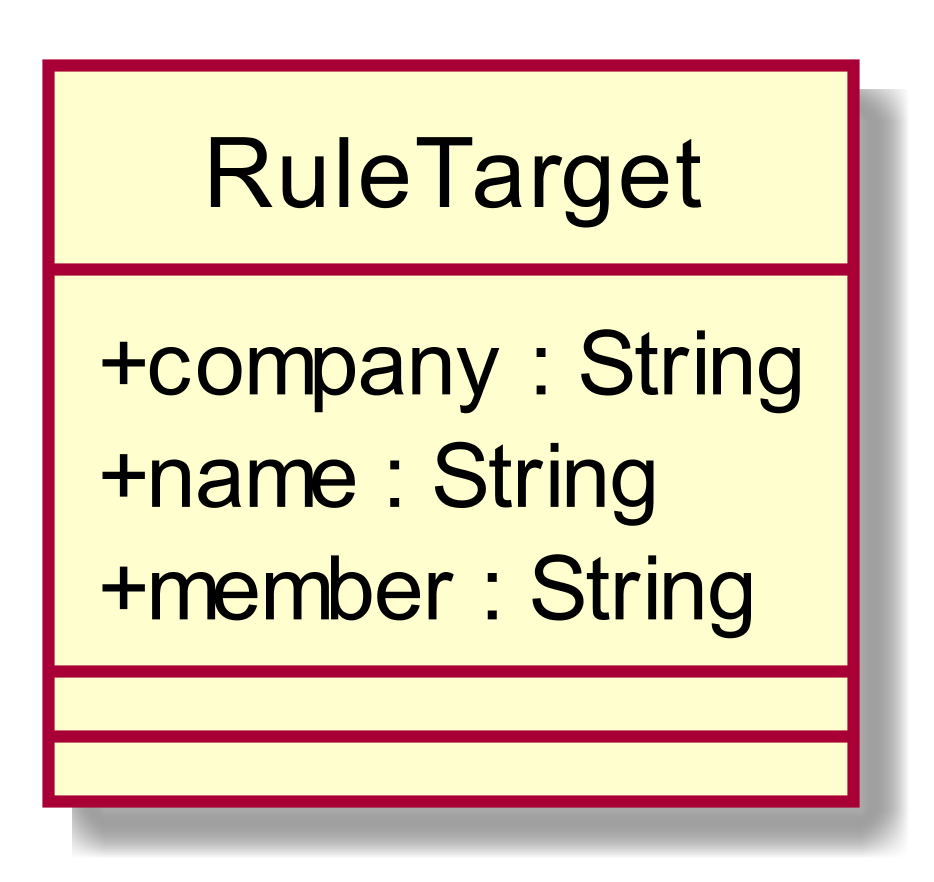
\includegraphics[width=0.35\textwidth,height=\textheight,keepaspectratio]{images/ClassRuleTarget.png}
	\caption{Back-end::Rules::RuleTarget}
\end{figure}
\begin{itemize}
	\item \textbf{Nome}: \file{RuleTarget};
	\item \textbf{Tipo}: \file{Class};
	\item \textbf{Descrizione}: questa classe si occupa di rappresentare e organizzare i dati relativi a un target di una \file{Rule}, ovvero la persona alla quale è indirizzata quest'ultima;
	\item \textbf{Utilizzo}: fornisce gli attributi di un target di una \file{Rule} che dovranno essere memorizzati nel database per questo microservizio.
	Viene utilizzata dalla classe \file{Rule} per definire un Array di \file{Target} ai quali applicare la sua funzione;
	\item \textbf{Attributi}:
	\begin{itemize}
		\item[] \file{+ company: String} \\
		Attributo contenente il nome dell'azienda;
		\item[] \file{+ name: String} \\
		Attributo contenente il nome del target;
		\item[] \file{+ member: String} \\
		Attributo contenente il nome del membro dell'azienda interessato dalla direttiva;
	\end{itemize}
	\item \textbf{Relazioni con le altre classi}:
	\begin{itemize}
		\item IN \hyperlink{Rule_label}{\file{Rule}}
	\end{itemize}
\end{itemize}
\FloatBarrier

\hypertarget{RuleTaskInstance_label}{\subparagraph{RuleTaskInstance}}
\begin{figure}[h]
	\centering
	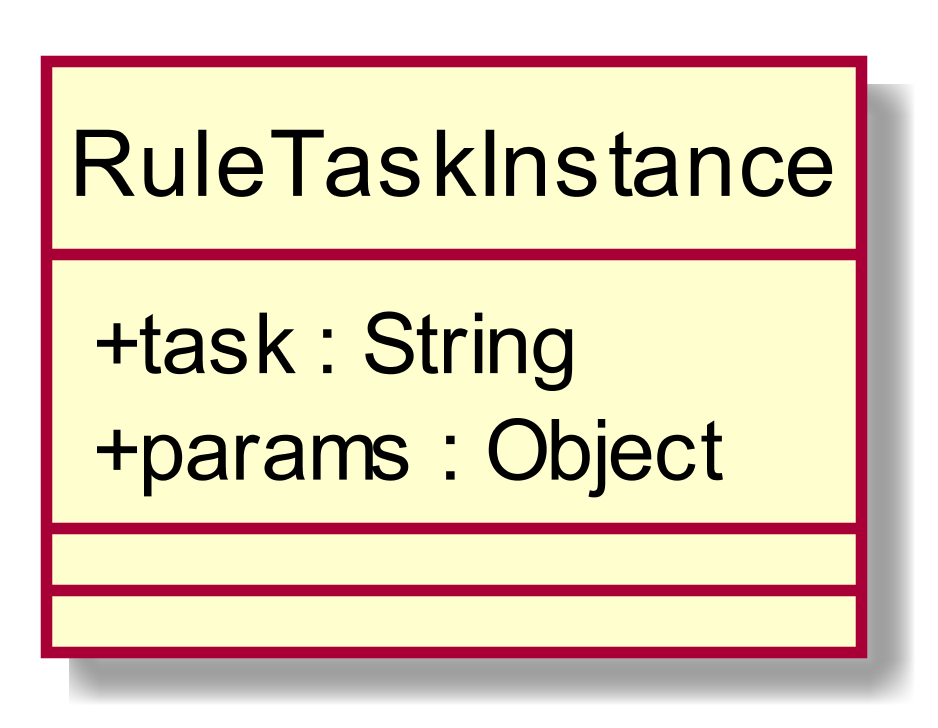
\includegraphics[width=0.35\textwidth,height=\textheight,keepaspectratio]{images/ClassRuleTaskInstance.png}
	\caption{Back-end::Rules::RuleTaskInstance}
\end{figure}
\begin{itemize}
	\item \textbf{Nome}: \file{RuleTaskInstance};
	\item \textbf{Tipo}: \file{Class};
	\item \textbf{Descrizione}: questa classe si occupa di rappresentare i dati relativi al compito di una direttiva;
	\item \textbf{Utilizzo}: fornisce un meccanismo per specificare la modifica di comportamento del sistema in seguito all'applicazione di una determinata direttiva;
	\item \textbf{Attributi}:
	\begin{itemize}
		\item[] \file{+ task: String} \\
		Attributo contenente il nome del Task da applicare;
		\item[] \file{+ params: Object} \\
		Attributo contenente i parametri da applicare alla funzione quando verrà chiamata;
	\end{itemize}
	\item \textbf{Relazioni con le altre classi}:
	\begin{itemize}
		\item IN \hyperlink{Rule_label}{\file{Rule}}
	\end{itemize}
\end{itemize}
\FloatBarrier

\hypertarget{Task_label}{\subparagraph{Task}}
\begin{figure}[h]
	\centering
	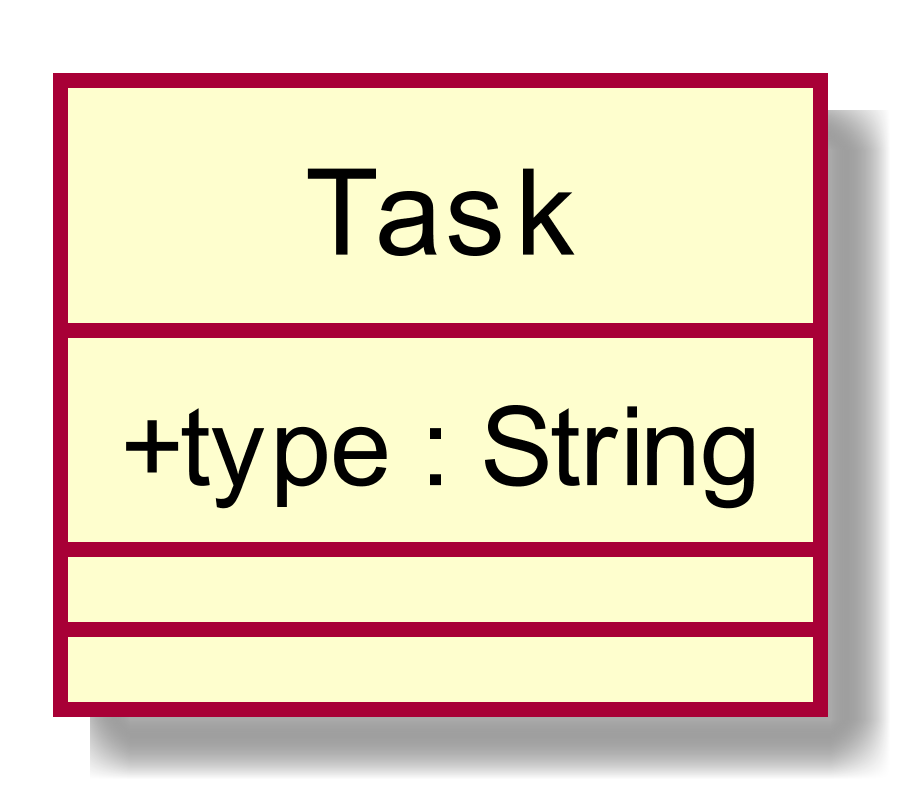
\includegraphics[width=0.35\textwidth,height=\textheight,keepaspectratio]{images/ClassTask.png}
	\caption{Back-end::Rules::Task}
\end{figure}
\begin{itemize}
	\item \textbf{Nome}: \file{Task};
	\item \textbf{Tipo}: \file{Class};
	\item \textbf{Descrizione}: questa classe si occupa di rappresentare la funzione che dovrà essere applicata ad una \file{Rule};
	\item \textbf{Utilizzo}: fornisce gli attributi delle funzioni (ovvero dei compiti che una certa \file{Rule} svolge) che dovranno essere applicate a certe \file{Rule}, i quali dovranno essere memorizzati nel database per questo microservizio;
	\item \textbf{Attributi}:
	\begin{itemize}
		\item[] \file{+ type: String} \\
		Attributo contenente il nome del Task;
	\end{itemize}
	\item \textbf{Relazioni con le altre classi}:
	\begin{itemize}
		\item IN \hyperlink{TaskObserver_label}{\file{TaskObserver}}
		\item IN \hyperlink{TasksDAODynamoDB_label}{\file{TasksDAODynamoDB}}
		\item IN \hyperlink{<<interface>> TasksDAO_label}{\file{<<interface>> TasksDAO}}
	\end{itemize}
\end{itemize}
\FloatBarrier

\hypertarget{TaskObservable_label}{\subparagraph{TaskObservable}}
\begin{figure}[h]
	\centering
	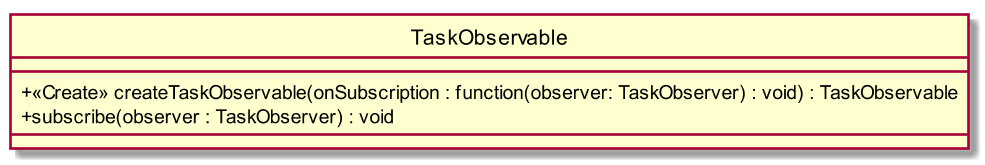
\includegraphics[width=\textwidth,height=\textheight,keepaspectratio]{images/ClassTaskObservable.png}
	\caption{Back-end::Rules::TaskObservable}
\end{figure}
\begin{itemize}
	\item \textbf{Nome}: \file{TaskObservable};
	\item \textbf{Tipo}: \file{Class};
	\item \textbf{Descrizione}: questa classe implementa un \file{Observable} che permette l'iscrizione di \file{TaskObserver};
	\item \textbf{Utilizzo}: fornisce i meccanismi necessari per il passaggio di una serie di \file{Task} ad un \file{Observer} interessato;
	\item \textbf{Padre}: \file{Observable};
	\item \textbf{Metodi}:
	\begin{itemize}
		\item[] \file{+ <<Create>> createTaskObservable(onSubscription: function(observer\\: TaskObserver) : void): TaskObservable} \\		Constructor di \file{TaskObservable};\\
		Parametri:
		\begin{itemize}
			\item \file{onSubscription: function(observer: TaskObserver) : void} \\
			Funzione che verrà eseguita quando un \file{Observer} si iscrive all'\file{Observable}. Si occupa di passare i dati all'\file{Observer}, chiamando il metodo \file{next(function: Task)}. Quando non ci sono più dati da restituire, si occupa di chiamare il metodo \file{complete}. Nel caso in cui si verificasse un errore, si occupa di chiamare il metodo \file{error(err: Object)} con i dati relativi all'errore verificatosi;
		\end{itemize}
		\item[] \file{+ subscribe(observer: TaskObserver): void} \\		Metodo che permette ad un \file{TaskObserver} interessato di iscriversi a questo \file{Observable};\\
		Parametri:
		\begin{itemize}
			\item \file{observer: TaskObserver} \\
			\file{Observer} che si vuole iscrivere;
		\end{itemize}
	\end{itemize}
	\item \textbf{Relazioni con le altre classi}:
	\begin{itemize}
		\item IN \hyperlink{<<interface>> TasksDAO_label}{\file{<<interface>> TasksDAO}}
		\item IN \hyperlink{TasksDAODynamoDB_label}{\file{TasksDAODynamoDB}}
		\item OUT \hyperlink{TaskObserver_label}{\file{TaskObserver}}
	\end{itemize}
\end{itemize}
\FloatBarrier

\hypertarget{TaskObserver_label}{\subparagraph{TaskObserver}}
\begin{figure}[h]
	\centering
	\includegraphics[width=0.35\textwidth,height=\textheight,keepaspectratio]{images/ClassTaskObserver.png}
	\caption{Back-end::Rules::TaskObserver}
\end{figure}
\begin{itemize}
	\item \textbf{Nome}: \file{TaskObserver};
	\item \textbf{Tipo}: \file{Class};
	\item \textbf{Descrizione}: classe che rappresenta un \file{Observer} che si aspetta dati di tipo \file{Task};
	\item \textbf{Utilizzo}: implementa il metodo \file{next} dell'interfaccia, in maniera tale che accetti dati di tipo \file{Task};
	\item \textbf{Metodi}:
	\begin{itemize}
		\item[] \file{+ next(task: Task): void} \\		Metodo che permette agli \file{Observable} di notificare l'\file{Observer} con dati di tipo \file{Task}. Definisce inoltre le operazioni che l'\file{Observer} compierà all'arrivo di tali dati;\\
		Parametri:
		\begin{itemize}
			\item \file{task: Task} \\
			Parametro contenente la \file{Task} mandata dall'\file{Observable};
		\end{itemize}
	\end{itemize}
	\item \textbf{Relazioni con le altre classi}:
	\begin{itemize}
		\item IN \hyperlink{TaskObservable_label}{\file{TaskObservable}}
		\item OUT \hyperlink{Task_label}{\file{Task}}
	\end{itemize}
\end{itemize}
\FloatBarrier

\hypertarget{TasksDAODynamoDB_label}{\subparagraph{TasksDAODynamoDB}}
\begin{figure}[h]
	\centering
	\includegraphics[width=0.75\textwidth,height=\textheight,keepaspectratio]{images/ClassTasksDAODynamoDB.png}
	\caption{Back-end::Rules::TasksDAODynamoDB}
\end{figure}
\begin{itemize}
	\item \textbf{Nome}: \file{TasksDAODynamoDB};
	\item \textbf{Tipo}: \file{Class};
	\item \textbf{Descrizione}: classe che si occupa di implementare l'interfaccia \file{TasksDAO}, utilizzando un database DynamoDB come supporto per la memorizzazione dei dati;
	\item \textbf{Utilizzo}: implementa i metodi dell'interfaccia \file{TasksDAO} interrogando un database DynamoDB. Utilizza \file{AWS::DynamoDB::DocumentClient} per l'accesso al database. La dependency injection dell'oggetto \file{AWS::DynamoDB} viene fatta utilizzando il costruttore;
	\item \textbf{Padre}: \file{<<interface>> TasksDAO};
	\item \textbf{Attributi}:
	\begin{itemize}
		\item[] \file{- client: AWS::DynamoDB::DocumentClient} \\
		Attributo contenente un riferimento al modulo di Node.js utilizzato per l'accesso al database DynamoDB contenente la tabella dei tasks;
	\end{itemize}
	\item \textbf{Metodi}:
	\begin{itemize}
		\item[] \file{+ addTask(task: Task): ErrorObservable} \\		Implementazione del metodo definito nell'interfaccia \file{TasksDAO}. Utilizza il metodo put del \file{DocumentClient} per aggiungere il \file{Task} al database;\\
		Parametri:
		\begin{itemize}
			\item \file{task: Task} \\
			Parametro contenente il \file{Task};
		\end{itemize}
		\item[] \file{+ getTask(id: String): TaskObservable} \\		Implementazione del metodo definito nell'interfaccia \file{TasksDAO}. Utilizza il metodo get del \file{DocumentClient} per ottenere i dati relativi ad una \file{Task} dal database;\\
		Parametri:
		\begin{itemize}
			\item \file{id: String} \\
			Parametro contenente l'id della funzione;
		\end{itemize}
		\item[] \file{+ getTaskList(): TaskObservable} \\		Implementazione del metodo dell'interfaccia \file{TasksDAO}. Utilizza il metodo scan del \\ \file{DocumentClient} per ottenere la lista dei \file{Task} dal database;\\
		\item[] \file{+ removeTask(id: String): ErrorObservable} \\		Implementazione del metodo dell'interfaccia \file{TasksDAO}. Utilizza il metodo delete del \file{DocumentClient} per eliminare un \file{Task} dal database;\\
		Parametri:
		\begin{itemize}
			\item \file{id: String} \\
			Parametro contenente l'id della funzione;
		\end{itemize}
		\item[] \file{+ updateTask(fun: Function): ErrorObservable} \\		Implementazione del metodo dell'interfaccia \file{TasksDAO}. Utilizza il metodo update del \file{DocumentClient} per aggiornare i dati relativi ad un \file{Task} presente all'interno del database;\\
		Parametri:
		\begin{itemize}
			\item \file{fun: Function} \\
			Parametro contenente la funzione;
		\end{itemize}
		\item[] \file{+ <<Create>> createTasksDAODynamoDB(client: AWS::DynamoDB::DocumentClient)\\: TasksDAODynamoDB} \\		Constructor della classe \file{TasksDAODynamoDB}. Permette di effettuare la dependency injection di \file{AWS::DynamoDB};\\
		Parametri:
		\begin{itemize}
			\item \file{client: AWS::DynamoDB::DocumentClient} \\
			Parametro contenente un riferimento al modulo di Node.js da utilizzare per l'accesso al database DynamoDB contenente la tabella delle funzioni;
		\end{itemize}
	\end{itemize}
	\item \textbf{Relazioni con le altre classi}:
	\begin{itemize}
		\item OUT \hyperlink{Task_label}{\file{Task}}
		\item OUT \hyperlink{TaskObservable_label}{\file{TaskObservable}}
		\item OUT \hyperlink{ErrorObservable_label}{\file{ErrorObservable}}
	\end{itemize}
\end{itemize}
\FloatBarrier

\newpage \subsubsection{Back-end::STT}
Package che include le classi che si occupano di fornire le funzionalità di \gl{Speech to text}.
\begin{figure}[h] \centering \includegraphics[width=\textwidth,height=\textheight,keepaspectratio]{images/diagrams/back-end/Official_Backend_0304/STT.png}
	\caption{Package Back-end::STT}
\end{figure}
\newpage

\paragraph{Classi}
\hypertarget{ STTModule_label}{\subparagraph{ STTModule}}
\begin{figure}[h]
	\centering
	\includegraphics[width=0.55\textwidth,height=\textheight,keepaspectratio]{images/ClassSTTModule.png}
	\caption{Back-end::STT:: STTModule}
\end{figure}
\begin{itemize}
	\item \textbf{Nome}: \file{ STTModule};
	\item \textbf{Tipo}: \file{Interface};
	\item \textbf{Descrizione}: classe che definisce l'interfaccia dei moduli utilizzati per le operazioni di Speech-To-Text (STT);
	\item \textbf{Utilizzo}: fornisce l'interfaccia che deve essere implementata dai moduli che permettono l'accesso alle funzionalità di STT;
	\item \textbf{Figlio}: \file{STTWatsonAdapter};
	\item \textbf{Metodi}:
	\begin{itemize}
		\item[] \file{+ speechToText(audio: Buffer, type: String): StringPromise} \\		Questo metodo permette di ricavare in modo asincrono il testo da un file audio. Viene utilizzato da \file{VocalAPI}, il quale invierà il testo ottenuto dall'invocazione di questo metodo all'assistente virtuale. Restituisce una promise che verrà soddisfatta con una stringa contenente il testo estratto;\\
		Parametri:
		\begin{itemize}
			\item \file{audio: Buffer} \\
			Buffer contenente l'audio da cui si vuole estrarre il testo;
			\item \file{type: String} \\
			Parametro contenete la descrizione del formato in cui i dati sono memorizzati in \file{audio};
		\end{itemize}
	\end{itemize}
	\item \textbf{Relazioni con le altre classi}:
	\begin{itemize}
		\item IN \hyperlink{VocalAPI_label}{\file{VocalAPI}}
	\end{itemize}
\end{itemize}
\FloatBarrier

\hypertarget{STTWatsonAdapter_label}{\subparagraph{STTWatsonAdapter}}
\begin{figure}[h]
	\centering
	\includegraphics[width=\textwidth,height=\textheight,keepaspectratio]{images/ClassSTTWatsonAdapter.png}
	\caption{Back-end::STT::STTWatsonAdapter}
\end{figure}
\begin{itemize}
	\item \textbf{Nome}: \file{STTWatsonAdapter};
	\item \textbf{Tipo}: \file{Class};
	\item \textbf{Descrizione}: questa classe si occupa di convertire l'interfaccia fornita dal servizio di Speech to Text di IBM in una più adatta alle esigenze dell'applicazione, definita da \file{STTModule}. \\
	Facendo da Adapter tra le API del servizio di Speech to Text di IBM (adaptee) e l'interfaccia \file{STTModule} (target) utilizzata da \file{APIGateway::VocalAPI}, permette l'interoperabilità tra queste due interfacce;
	\item \textbf{Utilizzo}: fornisce a \file{STTModule} un meccanismo che permette di interrogare le API del servizio Watson Speech to Text di IBM, in modo da consentire a \file{APIGateway::VocalAPI} l'utilizzo di quest'ultime utilizzando un'interfaccia distinta e più consona alle proprie esigenze.
	Per ulteriori informazioni, consultare le documentazioni presenti alle seguenti pagine:
	\begin{itemize}
		\item \url{https://www.ibm.com/watson/developercloud/doc/speech-to-text/}  (visitato in data 2017-03-21);
		\item \url{https://github.com/watson-developer-cloud/node-sdk#speech-to-text}  (visitato in data 2017-03-21).
	\end{itemize}
	\item \textbf{Padre}: \file{<<interface>> STTModule};
	\item \textbf{Attributi}:
	\begin{itemize}
		\item[] \file{- stt: SpeechToTextV1} \\
		Attributo contenente il \file{SpeechToTextV1Module}, creato a partire dai parametri \file{name} e \file{password} forniti al costruttore. Viene utilizzato per estrarre il contenuto testuale di un file audio utilizzando il servizio Watson Speech To Text di IBM;
		\item[] \file{- stream\_buffer: StreamBufferModule} \\
		Attributo contenente il \file{StreamBufferModule} di cui è stata effettuate la dependency injection nel costruttore. Viene utilizzata per creare un \file{ReadableStream} di node a partire da un buffer;
	\end{itemize}
	\item \textbf{Metodi}:
	\begin{itemize}
		\item[] \file{+ <<Create>> createSTTWatsonAdapter(sb: StreamBufferModule, stt: \\SpeechToTextV1): STTWatsonAdapter} \\		Costruttore di STTWatsonAdapter, che permette di effettuare la dependency injection di \file{StreamBufferModule} e di \file{SpeechToTextV1};\\
		Parametri:
		\begin{itemize}
			\item \file{sb: StreamBufferModule} \\
			Parametro tramite i quale si effettua la dependency injection di \file{StreamBufferModule};
			\item \file{stt: SpeechToTextV1} \\
			Parametro tramite il quale viene effettuata la dependency injection di \file{SpeechToTextV1};
		\end{itemize}
		\item[] \file{+ speechToText(audio: Buffer, type: String): StringPromise} \\			Implementa il metodo \file{speechToText} contenuto nell'interfaccia;\\
		Parametri:
		\begin{itemize}
			\item \file{audio: Buffer} \\
			Parametro contenente l'audio dal quale si vuole estrarre il testo;
			\item \file{type: String} \\
			Parametro contenente il formato in cui sono memorizzati i dati all'interno di \file{audio};
		\end{itemize}
	\end{itemize}
\end{itemize}
\FloatBarrier

\newpage \subsubsection{Back-end::Users}
Package contenente le classi e le interfacce che realizzano il microservizio di autenticazione e registrazione di un amministratore nel sistema.\\
Vengono offerte funzionalità che permettono:
\begin{itemize}
	\item la registrazione di un nuovo amministratore;
	\item l'autenticazione di un amministratore;
	\item gestione degli amministratori esistenti.
\end{itemize}
\begin{figure}[h] \centering \includegraphics[width=\textwidth,height=\textheight,keepaspectratio]{images/diagrams/back-end/Official_Backend_0304/Users.png}
	\caption{Package Back-end::Users}
\end{figure}
\newpage

\paragraph{Classi}
\hypertarget{ UsersDAO_label}{\subparagraph{ UsersDAO}}
\begin{figure}[h]
	\centering
	\includegraphics[width=0.50\textwidth,height=\textheight,keepaspectratio]{images/ClassUsersDAO.png}
	\caption{Back-end::Users:: UsersDAO}
\end{figure}
\begin{itemize}
	\item \textbf{Nome}: \file{ UsersDAO};
	\item \textbf{Tipo}: \file{Interface};
	\item \textbf{Descrizione}: questa classe si occupa di astrarre le modalità d'interazione al database per questo microservizio;
	\item \textbf{Utilizzo}: fornisce a \file{UsersService} un meccanismo per accedere al database contenente gli utenti registrati, senza conoscerne le modalità di implementazione e di persistenza di quest'ultimo.
	A partire da un identificativo, permette operazioni di lettura, scrittura e rimozione di utenti registrati;
	\item \textbf{Figlio}: \file{UsersDAODynamoDB};
	\item \textbf{Metodi}:
	\begin{itemize}
		\item[] \file{+ addUser(user: User): ErrorObservable} \\		Metodo che permette di aggiungere un utente. \\
		L'\file{Observable} restituito non riceverà alcun valore, ma verrà completato in caso di aggiunta dell'utente avvenuta con successo. In caso di errore durante l'aggiunta dell'utente, gli \file{Observer} interessati verranno notificati tramite la chiamata del loro metodo \file{error} con i dati relativi all'errore verificatosi;\\
		Parametri:
		\begin{itemize}
			\item \file{user: User} \\
			Parametro contenente un utente registrato;
		\end{itemize}
		\item[] \file{+ removeUser(id: String): ErrorObservable} \\		Metodo che permette di rimuovere un utente registrato. L'\file{Observable} restituito non riceverà alcun valore, ma verrà completato in caso di aggiunta dell'utente avvenuta con successo. In caso di errore durante l'aggiunta dell'utente, gli \file{Observer} interessati verranno notificati tramite la chiamata del loro metodo \file{error} con i dati relativi all'errore verificatosi;\\
		Parametri:
		\begin{itemize}
			\item \file{id: String} \\
			Parametro contenente l'id dello \file{User} che si vuole eliminare;
		\end{itemize}
		\item[] \file{+ getUser(username: String): UserObservable} \\		Metodo che permette di ottenere i dati relativi ad un utente. \\
		L'\file{Observable} restituito riceverà l'oggetto rappresentante tale \file{User}, e verrà completato. Nel caso in cui l'utente richiesto non sia presente nel database, gli \file{Observer} interessati non riceveranno alcun valore, ma verranno notificati tramite la chiamata del loro metodo \file{error};\\
		Parametri:
		\begin{itemize}
			\item \file{username: String} \\
			Parametro contenente lo username dello \file{User} che si vuole ottenere;
		\end{itemize}
		\item[] \file{+ getUserList(): UserObservable} \\		L'\file{Observable} restituito manderà agli \file{Observer} gli utenti ottenuti, uno alla volta, e poi chiama il loro metodo \file{complete}. Nel caso in cui si verifichi un errore, gli \file{Observer} iscritti verranno notificati tramite la chiamate del loro metodo \file{error} con i dati relativi all'errore verificatosi;\\
		\item[] \file{+ updateUser(user: User): ErrorObservable} \\		Metodo che permette di aggiornare un utente registrato.  L'\file{Observable} restituito non riceverà alcun valore, ma verrà completato in caso di aggiunta dell'utente avvenuta con successo. In caso di errore durante l'aggiunta dell'utente, gli \file{Observer} interessati verranno notificati tramite la chiamata del loro metodo \file{error} con i dati relativi all'errore verificatosi;\\
		Parametri:
		\begin{itemize}
			\item \file{user: User} \\
			Parametro contenente lo \file{User} aggiornato;
		\end{itemize}
	\end{itemize}
	\item \textbf{Relazioni con le altre classi}:
	\begin{itemize}
		\item IN \hyperlink{AdministrationWebhookService_label}{\file{AdministrationWebhookService}}
		\item IN \hyperlink{ConversationWebhookService_label}{\file{ConversationWebhookService}}
		\item IN \hyperlink{UsersService_label}{\file{UsersService}}
		\item OUT \hyperlink{User_label}{\file{User}}
		\item OUT \hyperlink{UserObservable_label}{\file{UserObservable}}
		\item OUT \hyperlink{ErrorObservable_label}{\file{ErrorObservable}}
	\end{itemize}
\end{itemize}
\FloatBarrier

\hypertarget{VocalLoginModule_label}{\subparagraph{VocalLoginModule}}
\begin{figure}[h]
	\centering
	\includegraphics[width=0.50\textwidth,height=\textheight,keepaspectratio]{images/ClassVocalLoginModule.png}
	\caption{Back-end::Users::VocalLoginModule}
\end{figure}
\begin{itemize}
	\item \textbf{Nome}: \file{VocalLoginModule};
	\item \textbf{Tipo}: \file{Interface};
	\item \textbf{Descrizione}: interfaccia che rappresenta un modulo di Node.js che viene utilizzato per il login vocale degli utenti;
	\item \textbf{Utilizzo}: viene implementata dai moduli utilizzati per il login vocale degli utenti;
	\item \textbf{Figlio}: \file{VocalLoginMicrosoftModule};
	\item \textbf{Metodi}:
	\begin{itemize}
		\item[] \file{+ createUser(): StringObservable} \\		Metodo che permette di creare un \file{User};\\
		\item[] \file{+ addEnrollment(id: String, audio: Blob): ErrorObservable} \\		Metodo che permette di aggiungere un \file{Enrollment};\\
		Parametri:
		\begin{itemize}
			\item \file{id: String} \\
			Parametro contenente la stringa identificativa dell'utente al quale si vuole aggiungere un \file{Enrollment};
			\item \file{audio: Blob} \\
			Parametro contenente l'audio relativo alla frase di riconoscimento pronunciata;
		\end{itemize}
		\item[] \file{+ deleteUser(id: String): ErrorObservable} \\		Metodo che permette di eliminare un \file{User} a partire da un id;\\
		Parametri:
		\begin{itemize}
			\item \file{id: String} \\
			Parametro contenente l'identificativo dell'utente che si vuole eliminare;
		\end{itemize}
		\item[] \file{+ getList(): SRUserArray} \\		Metodo che ritorna una lista di \file{SRUser};\\
		\item[] \file{+ getUser(id: String): SRUser} \\		Metodo che ritorna un \file{SRUser} a partire da un id;\\
		Parametri:
		\begin{itemize}
			\item \file{id: String} \\
			Parametro contenente l'identificativo dello \file{User};
		\end{itemize}
		\item[] \file{+ resetEnrollments(id: String): ErrorObservable} \\		Metodo che permette di resettare un \file{Enrollment} a partire da un id;\\
		Parametri:
		\begin{itemize}
			\item \file{id: String} \\
			Parametro contenente l'identificativo dell'utente dei quali relativi enrollment verrà effettuato il reset;
		\end{itemize}
		\item[] \file{+ doLogin(id: String, audio: Blob): ErrorObservable} \\		Metodo che permette di effettuare il login a partire da un id e da un audio di identificazione;\\
		Parametri:
		\begin{itemize}
			\item \file{id: String} \\
			Parametro contenente l'identificativo dell'utente che vuole effettuare il login;
			\item \file{audio: Blob} \\
			Parametro contenente l'audio relativo alla frase di riconoscimento pronunciata;
		\end{itemize}
	\end{itemize}
	\item \textbf{Relazioni con le altre classi}:
	\begin{itemize}
		\item IN \hyperlink{VocalAPI_label}{\file{VocalAPI}}
		\item OUT \hyperlink{SRUser_label}{\file{SRUser}}
	\end{itemize}
\end{itemize}
\FloatBarrier

\hypertarget{SRUser_label}{\subparagraph{SRUser}}
\begin{figure}[h]
	\centering
	\includegraphics[width=0.35\textwidth,height=\textheight,keepaspectratio]{images/ClassSRUser.png}
	\caption{Back-end::Users::SRUser}
\end{figure}
\begin{itemize}
	\item \textbf{Nome}: \file{SRUser};
	\item \textbf{Tipo}: \file{Class};
	\item \textbf{Descrizione}: questa classe si occupa di rappresentare ed organizzare i parametri dell'autenticazione tramite Speaker Recognition (SR);
	\item \textbf{Utilizzo}: fornisce l'insieme dei parametri necessari ad identificare, tramite SR, un utente sottoposto alla procedura di Enrollment del servizio di Speaker Recognition.
	Per la relativa documentazione consultare la pagina \url{https://www.microsoft.com/cognitive-services/en-us/speaker-recognition-api/documentation}  (visitato in data 2017-03-21).
	;
	\item \textbf{Attributi}:
	\begin{itemize}
		\item[] \file{+ id: String} \\
		Attributo contenente l'identificativo del profilo utente del microservizio di Speaker Recognition;
		\item[] \file{+ enrollmentCount: int} \\
		Attributo contenente il numero di Enrollment dello \file{User};
		\item[] \file{+ createdDateTime: String} \\
		Attributo contenente la data di creazione del profilo utente nel microservizio esterno di Speaker Recognition;
		\item[] \file{+ enrollmentStatus: String} \\
		Attributo contenente lo stato dell'Enrollment.\\
		Lo stato può essere uno tra i seguenti valori:
		\begin{itemize} \item Enrolling: indica che la fase di enrollment è in corso; \item Training: indica che il microservizio di Speaker Recognition sta elaborando e organizzando i dati ricevuti (analizza le frasi comunicate e ne costruisce un'impronta vocale); \item Enrolled, ovvero che le due fasi precedenti sono state completate. \end{itemize}
	\end{itemize}
	\item \textbf{Relazioni con le altre classi}:
	\begin{itemize}
		\item IN \hyperlink{<<interface>>VocalLoginModule_label}{\file{<<interface>>VocalLoginModule}}
	\end{itemize}
\end{itemize}
\FloatBarrier

\hypertarget{User_label}{\subparagraph{User}}
\begin{figure}[h]
	\centering
	\includegraphics[width=0.55\textwidth,height=\textheight,keepaspectratio]{images/ClassUser.png}
	\caption{Back-end::Users::User}
\end{figure}
\begin{itemize}
	\item \textbf{Nome}: \file{User};
	\item \textbf{Tipo}: \file{Class};
	\item \textbf{Descrizione}: questa classe si occupa di rappresentare e organizzare i dati relativi ad un utente registrato;
	\item \textbf{Utilizzo}: fornisce i metodi getter e setter per i parametri relativi ad un utente registrato, i quali dovranno essere memorizzati nel database per questo microservizio.\\
	È utilizzata dalla classe \file{UsersDAO} e dalle classi che utilizzano quest'ultima;
	\item \textbf{Attributi}:
	\begin{itemize}
		\item[] \file{- username: String} \\
		Attributo contenente l'username dell'utente registrato;
		\item[] \file{- name: String} \\
		Attributo contenente il nome e cognome dell'utente registrato;
		\item[] \file{- password: String[0..1]} \\
		Attributo contenente la password dell'utente registrato;
		\item[] \file{- slack\_channel: String[0..1]} \\
		Attributo contenente il canale Slack dell'utente registrato;
		\item[] \file{- sr\_id: String[0..1]} \\
		Attributo contenente l'id del profilo utente nel microservizio esterno di Speaker Recognition;
	\end{itemize}
	\item \textbf{Metodi}:
	\begin{itemize}
		\item[] \file{+ getId(): String} \\		Metodo che permette di ottenere l'id dell'utente registrato;\\
		\item[] \file{+ setId(id: String): void} \\		Metodo che permette di impostare l'id dell'utente registrato;\\
		Parametri:
		\begin{itemize}
			\item \file{id: String} \\
			Parametro contenente l'id;
		\end{itemize}
		\item[] \file{+ getUsername(): String} \\		Metodo che permette di ottenere lo username dell'utente registrato;\\
		\item[] \file{+ setUsername(username: String): void} \\		Metodo che permette di impostare lo username dell'utente registrato;\\
		Parametri:
		\begin{itemize}
			\item \file{username: String} \\
			Parametro relativo all'username da settare;
		\end{itemize}
		\item[] \file{+ getNome(): String} \\		Metodo che permette di ottenere il nome dell'utente registrato;\\
		\item[] \file{+ setNome(nome: String): void} \\		Metodo che permette di impostare il nome dell'utente registrato;\\
		Parametri:
		\begin{itemize}
			\item \file{nome: String} \\
			Parametro contenente il nome;
		\end{itemize}
		\item[] \file{+ getPassword(): String[0..1]} \\		Metodo che permette di ottenere la password dell'utente registrato;\\
		\item[] \file{+ setPassword(password: String[0..1]): void} \\		Metodo che permette di impostare la password dell'utente registrato;\\
		Parametri:
		\begin{itemize}
			\item \file{password: String[0..1]} \\
			Parametro relativo alla password da settare;
		\end{itemize}
		\item[] \file{+ getSlackChannel(): String[0..1]} \\		Metodo che permette di ottenere il canale Slack dell'utente registrato;\\
		\item[] \file{+ setSlackChannel(slack\_channel: String[0..1]): void} \\		Metodo che permette di impostare il canale Slack dell'utente registrato necessario per contattarlo;\\
		Parametri:
		\begin{itemize}
			\item \file{slack\_channel: String[0..1]} \\
			Parametro relativo al canale Slack da settare;
		\end{itemize}
		\item[] \file{+ getSrId(): String[0..1]} \\		Metodo che permette di ottenere l'id del profilo utente nel microservizio esterno di Speaker Recognition;\\
		\item[] \file{+ setSrId(sr\_id: String[0..1]): void} \\		Metodo che permette di impostare l'id dello Speaker Recognition associato all'utente registrato;\\
		Parametri:
		\begin{itemize}
			\item \file{sr\_id: String[0..1]} \\
			Parametro relativo all'id dello Speaker Recognition da settare;
		\end{itemize}
	\end{itemize}
	\item \textbf{Relazioni con le altre classi}:
	\begin{itemize}
		\item IN \hyperlink{<<interface>> UsersDAO_label}{\file{<<interface>> UsersDAO}}
		\item IN \hyperlink{UserObserver_label}{\file{UserObserver}}
		\item IN \hyperlink{UsersDAODynamoDB_label}{\file{UsersDAODynamoDB}}
		\item IN \hyperlink{VocalAPI_label}{\file{VocalAPI}}
	\end{itemize}
\end{itemize}
\FloatBarrier

\hypertarget{UserObservable_label}{\subparagraph{UserObservable}}
\begin{figure}[h]
	\centering
	\includegraphics[width=\textwidth,height=\textheight,keepaspectratio]{images/ClassUserObservable.png}
	\caption{Back-end::Users::UserObservable}
\end{figure}
\begin{itemize}
	\item \textbf{Nome}: \file{UserObservable};
	\item \textbf{Tipo}: \file{Class};
	\item \textbf{Descrizione}: questa classe implementa un \file{Observable} che permette l'iscrizione di \file{UserObserver};
	\item \textbf{Utilizzo}: fornisce i meccanismi necessari per il passaggio di una serie di \file{User} ad un \file{Observer} interessato;
	\item \textbf{Padre}: \file{Observable};
	\item \textbf{Metodi}:
	\begin{itemize}
		\item[] \file{+ subscribe(observer: UserObserver): Subscription} \\		Metodo che permette ad uno \file{UserObserver} interessato di iscriversi a questo \file{Observable};\\
		Parametri:
		\begin{itemize}
			\item \file{observer: UserObserver} \\
			\file{Observer} che si vuole iscrivere;
		\end{itemize}
		\item[] \file{+ <<Create>> createUserObservable(onSubscription: function(observer\\: UserObserver) : void): UserObservable} \\		Constructor di \file{UserObservable};\\
		Parametri:
		\begin{itemize}
			\item \file{onSubscription: function(observer: UserObserver) : void} \\
			Funzione che verrà eseguita quando un \file{Observer} si iscrive all'\file{Observable}. Si occupa di passare i dati all'\file{Observer}, chiamando il metodo \file{next(user: User)}. Quando non ci sono più dati da restituire, si occupa di chiamare il metodo \file{complete}. Nel caso in cui si verificasse un errore, si occupa di chiamare il metodo \file{error(err: Object)} con i dati relativi all'errore verificatosi;
		\end{itemize}
	\end{itemize}
	\item \textbf{Relazioni con le altre classi}:
	\begin{itemize}
		\item IN \hyperlink{<<interface>> UsersDAO_label}{\file{<<interface>> UsersDAO}}
		\item IN \hyperlink{UsersDAODynamoDB_label}{\file{UsersDAODynamoDB}}
		\item OUT \hyperlink{UserObserver_label}{\file{UserObserver}}
	\end{itemize}
\end{itemize}
\FloatBarrier

\hypertarget{UserObserver_label}{\subparagraph{UserObserver}}
\begin{figure}[h]
	\centering
	\includegraphics[width=0.35\textwidth,height=\textheight,keepaspectratio]{images/ClassUserObserver.png}
	\caption{Back-end::Users::UserObserver}
\end{figure}
\begin{itemize}
	\item \textbf{Nome}: \file{UserObserver};
	\item \textbf{Tipo}: \file{Class};
	\item \textbf{Descrizione}: classe che rappresenta un \file{Observer} che si aspetta dati di tipo \file{User};
	\item \textbf{Utilizzo}: ridefinisce il metodo \file{next} della classe \file{ObserverAdapter}, in maniera tale che accetti dati di tipo \file{User};
	\item \textbf{Metodi}:
	\begin{itemize}
		\item[] \file{+ next(user: User): void} \\		Metodo che permette agli \file{Observable} di notificare l'\file{Observer} con dati di tipo \file{User}. Definisce inoltre le operazioni che l'\file{Observer} compierà all'arrivo di tali dati;\\
		Parametri:
		\begin{itemize}
			\item \file{user: User} \\
			Parametro contenente lo \file{User} mandato dall'\file{Observable};
		\end{itemize}
	\end{itemize}
	\item \textbf{Relazioni con le altre classi}:
	\begin{itemize}
		\item IN \hyperlink{UserObservable_label}{\file{UserObservable}}
		\item OUT \hyperlink{User_label}{\file{User}}
	\end{itemize}
\end{itemize}
\FloatBarrier

\hypertarget{UsersDAODynamoDB_label}{\subparagraph{UsersDAODynamoDB}}
\begin{figure}[h]
	\centering
	\includegraphics[width=0.80\textwidth,height=\textheight,keepaspectratio]{images/ClassUsersDAODynamoDB.png}
	\caption{Back-end::Users::UsersDAODynamoDB}
\end{figure}
\begin{itemize}
	\item \textbf{Nome}: \file{UsersDAODynamoDB};
	\item \textbf{Tipo}: \file{Class};
	\item \textbf{Descrizione}: classe che si occupa di implementare l'interfaccia \file{UsersDAO}, utilizzando un database DynamoDB come supporto per la memorizzazione dei dati;
	\item \textbf{Utilizzo}: implementa i metodi dell'interfaccia \file{UsersDAO} interrogando un database DynamoDB. Utilizza \file{AWS::DynamoDB::DocumentClient} per l'accesso al database. La dependency injection dell'oggetto \file{AWS::DynamoDB} viene fatta utilizzando il costruttore;
	\item \textbf{Padre}: \file{<<interface>> UsersDAO};
	\item \textbf{Attributi}:
	\begin{itemize}
		\item[] \file{- client: AWS::DynamoDB::DocumentClient} \\
		Attributo contenente un riferimento al modulo di Node.js utilizzato per l'accesso al database DynamoDB contenente la tabella degli utenti;
	\end{itemize}
	\item \textbf{Metodi}:
	\begin{itemize}
		\item[] \file{+ addUser(user: User): ErrorObservable} \\		Implementazione del metodo definito nell'interfaccia \file{UsersDAO}. Utilizza il metodo \file{put} del \file{DocumentClient} per aggiungere l'utente al database;\\
		Parametri:
		\begin{itemize}
			\item \file{user: User} \\
			Utente che si vuole aggiungere al sistema;
		\end{itemize}
		\item[] \file{+ getUser(username: String): UserObservable} \\		Implementazione del metodo definito nell'interfaccia \file{UsersDAO}. Utilizza il metodo \file{get} del \file{DocumentClient} per ottenere i dati relativi ad uno \file{User} dal database;\\
		Parametri:
		\begin{itemize}
			\item \file{username: String} \\
			Parametro contenente lo \file{username} dello \file{User} che si vuole ottenere;
		\end{itemize}
		\item[] \file{+ getUserList(): UserObservable} \\		Implementazione del metodo dell'interfaccia \file{UsersDAO}. Utilizza il metodo \file{scan} del \file{DocumentClient} per ottenere la lista degli utenti dal database;\\
		\item[] \file{+ removeUser(username: String): ErrorObservable} \\		Implementazione del metodo dell'interfaccia \file{UsersDAO}. Utilizza il metodo \file{delete} del \file{DocumentClient} per eliminare un utente dal database;\\
		Parametri:
		\begin{itemize}
			\item \file{username: String} \\
			Parametro contenente lo \file{username} dello \file{User} che si vuole rimuovere;
		\end{itemize}
		\item[] \file{+ updateUser(user: User): ErrorObservable} \\		Implementazione del metodo dell'interfaccia \file{UsersDAO}. Utilizza il metodo \file{update} del \file{DocumentClient} per aggiornare i dati relativi ad un utente presente all'interno del database;\\
		Parametri:
		\begin{itemize}
			\item \file{user: User} \\
			Parametro contenente i dati relativi all'utente che si vuole modificare;
		\end{itemize}
		\item[] \file{+ <<Create>> createUsersDAODynamoDB(client: AWS::DynamoDB::DocumentClient)\\: UsersDAODynamoDB} \\		Constructor della classe \file{UsersDAODynamoDB}. Permette di effettuare la dependency injection di \file{AWS::DynamoDB::DocumentClient};\\
		Parametri:
		\begin{itemize}
			\item \file{client: AWS::DynamoDB::DocumentClient} \\
			Parametro contenente un riferimento al modulo di Node.js da utilizzare per l'accesso al database DynamoDB contenente la tabella degli utenti;
		\end{itemize}
	\end{itemize}
	\item \textbf{Relazioni con le altre classi}:
	\begin{itemize}
		\item OUT \hyperlink{User_label}{\file{User}}
		\item OUT \hyperlink{UserObservable_label}{\file{UserObservable}}
		\item OUT \hyperlink{ErrorObservable_label}{\file{ErrorObservable}}
	\end{itemize}
\end{itemize}
\FloatBarrier

\hypertarget{UsersService_label}{\subparagraph{UsersService}}
\begin{figure}[h]
	\centering
	\includegraphics[width=0.50\textwidth,height=\textheight,keepaspectratio]{images/ClassUsersService.png}
	\caption{Back-end::Users::UsersService}
\end{figure}
\begin{itemize}
	\item \textbf{Nome}: \file{UsersService};
	\item \textbf{Tipo}: \file{Class};
	\item \textbf{Descrizione}: questa classe si occupa di realizzare il microservizio \file{Users} e, tramite \file{UsersDAO}, di interagire con il database degli utenti registrati;
	\item \textbf{Utilizzo}: fornisce i metodi che implementano le Lambda Function necessarie alla gestione degli utenti.
	Questa classe non interagisce direttamente con il database, ma fa utilizzo di \file{UsersDAO}, il quale nasconde i meccanismi di accesso e persistenza dei dati nel database;
	\item \textbf{Attributi}:
	\begin{itemize}
		\item[] \file{- users: UsersDAO} \\
		Attributo che permette di contattare \file{UsersDAO}, il quale fornisce i meccanismi d'accesso al database degli utenti registrati;
	\end{itemize}
	\item \textbf{Metodi}:
	\begin{itemize}
		\item[] \file{+ getUserList(event: LambdaEvent, context: LambdaContext): void} \\\\		Metodo che implementa la Lambda Function che si occupa di restituire l'array degli utenti registrati;\\
		Parametri:
		\begin{itemize}
			\item \file{event: LambdaEvent} \\
			Parametro che rappresenta la richiesta ricevuta dal \file{VocalAPI}. Il campo \file{body} di questo attributo conterrà una stringa vuota;
			\item \file{context: LambdaContext} \\
			Parametro utilizzato dalle Lambda Function per inviare la risposta. Il \file{body} del \file{LambdaResponse}, ottenuto dal metodo \file{LambdaContext::succeed}, conterrà un Array di oggetti di tipo \file{User};
		\end{itemize}
		\item[] \file{+ addUser(event: LambdaEvent, context: LambdaContext): void} \\		Metodo che implementa la Lambda Function che si occupa di aggiungere un utente registrato;\\
		Parametri:
		\begin{itemize}
			\item \file{event: LambdaEvent} \\
			Parametro contenente, all'interno del campo \file{body} sotto forma di stringa in formato JSON, un oggetto \file{User} contenente tutti i dati relativi ad un utente da inserire;
			\item \file{context: LambdaContext} \\
			Parametro utilizzato dalle Lambda Function per inviare la risposta. La risposta, contenuta nel \file{LambdaResponse} parametro del metodo \file{LambdaContext::succeed}, possiede un attributo \file{body}, il quale conterrà una stringa vuota. Il risultato delle operazioni di questo metodo sarà deducibile tramite il valore dell'attributo \\ \file{LambaResponse::statusCode};
		\end{itemize}
		\item[] \file{+ deleteUser(event: LambdaIdEvent, context: LambdaContext): void}\\ \\		Metodo che implementa la Lambda Function che si occupa di rimuovere un utente registrato;\\
		Parametri:
		\begin{itemize}
			\item \file{event: LambdaIdEvent} \\
			Parametro contenente, all'interno del campo \file{pathParameters}, lo username dell'utente registrato che si vuole eliminare;
			\item \file{context: LambdaContext} \\
			Parametro utilizzato dalle Lambda Function per inviare la risposta. Il \file{body} del \file{LambdaResponse}, parametro del metodo \file{LambdaContext::succeed}, conterrà una stringa vuota e il risultato di questa operazione sarà deducibile dal valore dell'attributo \file{LambaResponse::statusCode};
		\end{itemize}
		\item[] \file{+ updateUser(event: LambdaIdEvent, context: LambdaContext): void}\\ \\		Metodo che implementa la Lambda Function che si occupa di aggiornare i dati di un utente registrato;\\
		Parametri:
		\begin{itemize}
			\item \file{event: LambdaIdEvent} \\
			Parametro contenente all'interno del campo \file{body}, sotto forma di stringa in formato JSON, un oggetto di tipo \file{User} contente i dati da aggiornare e, all'interno del campo \file{pathParameters}, lo username dell'utente da modificare;
			\item \file{context: LambdaContext} \\
			Parametro utilizzato dalle Lambda Function per inviare la risposta. Il \file{body} del \file{LambdaResponse}, parametro del metodo \file{LambdaContext::succeed}, conterrà una stringa vuota e il risultato di questa operazione sarà deducibile dal valore dell'attributo \file{LambaResponse::statusCode};
		\end{itemize}
		\item[] \file{+ getUser(event: LambdaIdEvent, context: LambdaContext): void} \\\\		Metodo che implementa la Lambda Function che si occupa di restituire i dati relativi ad un utente a partire dal suo \file{username};\\
		Parametri:
		\begin{itemize}
			\item \file{event: LambdaIdEvent} \\
			Parametro contenente, all'interno del campo \file{pathParameters}, lo username dell'utente registrato del quale si vogliono ottenere i dati;
			\item \file{context: LambdaContext} \\
			Parametro utilizzato dalle Lambda Function per inviare la risposta. Il \file{body} del \file{LambdaResponse}, parametro del metodo \file{LambdaContext::succeed}, conterrà un oggetto, sotto forma di stringa in formato JSON, di tipo \file{User}, contenente i dati relativi all'utente ritornato;
		\end{itemize}
		\item[] \file{+ <<create>> createUsersService(user: UserDAO): UsersService} \\		Metodo che permette di creare uno \file{UsersService}. Permette la dependency injection avente come oggetto uno \file{UsersDAO};\\
		Parametri:
		\begin{itemize}
			\item \file{user: UserDAO} \\
			Attributo contenente lo \file{UsersDAO};
		\end{itemize}
	\end{itemize}
	\item \textbf{Relazioni con le altre classi}:
	\begin{itemize}
		\item OUT \hyperlink{LambdaContext_label}{\file{LambdaContext}}
		\item OUT \hyperlink{LambdaIdEvent_label}{\file{LambdaIdEvent}}
		\item OUT \hyperlink{<<interface>> UsersDAO_label}{\file{<<interface>> UsersDAO}}
		\item OUT \hyperlink{LambdaEvent_label}{\file{LambdaEvent}}
	\end{itemize}
\end{itemize}
\FloatBarrier

\hypertarget{VocalLoginMicrosoftModule_label}{\subparagraph{VocalLoginMicrosoftModule}}
\begin{figure}[h]
	\centering
	\includegraphics[width=0.80\textwidth,height=\textheight,keepaspectratio]{images/ClassVocalLoginMicrosoftModule.png}
	\caption{Back-end::Users::VocalLoginMicrosoftModule}
\end{figure}
\begin{itemize}
	\item \textbf{Nome}: \file{VocalLoginMicrosoftModule};
	\item \textbf{Tipo}: \file{Class};
	\item \textbf{Descrizione}: questa classe si occupa di realizzare e raggruppare tutte le operazioni necessarie all'identificazione di un utente registrato, tramite il microservizio di Speaker Recognition (SR) di Microsoft;
	\item \textbf{Utilizzo}: fornisce un meccanismo per creare, eliminare ed ottenere un utente registrato associato ad un \file{Enrollment}, il quale è necessario all'identificazione di un utente tramite il microservizio di Speak Recognition (SR). Permette quindi di associare i parametri relativi ad un \file{Enrollment} ad un utente registrato.\\
	È soggetta ad una constructor-based dependency injection, la quale ha come oggetto un \file{RequestPromiseModule};
	\item \textbf{Padre}: \file{<<interface>>VocalLoginModule};
	\item \textbf{Attributi}:
	\begin{itemize}
		\item[] \file{- min\_confidence: int} \\
		Attributo contenente il grado di confidenza minimo accettabile nel confronto tra ciò che l'utente comunica, al fine di effettuare l'accesso come utente registrato, e quella che dovrebbe essere la sua impronta vocale precedentemente costruita tramite il meccanismo di \file{Enrollment};
		\item[] \file{- request\_promise: RequestPromiseModule} \\
		Attributo contenente il modulo Node.js \file{RequestPromiseModule}, utilizzato dalla classe per effettuare le richieste http alle API;
		\item[] \file{- key: String} \\
		Chiave di accesso alle API di Speaker Recognition di Microsoft;
	\end{itemize}
	\item \textbf{Metodi}:
	\begin{itemize}
		\item[] \file{+ <<Create>> createVocalLoginModule(conf: VocalLoginModuleConfig,\\ rp: RequestPromiseModule): VocalLoginModule} \\		Metodo che permette di costruire un \file{VocalLoginModule}. Permette la dependency injection che ha come oggetto un \file{VocalLoginModuleConfig};\\
		Parametri:
		\begin{itemize}
			\item \file{conf: VocalLoginModuleConfig} \\
			Parametro attraverso il quale viene passata la configurazione di \file{VocalLoginModule};
			\item \file{rp: RequestPromiseModule} \\
			Parametro attraverso il quale viene effettuata la dependency injection di \\  \file{RequestPromiseModule};
		\end{itemize}
		\item[] \file{+ addEnrollment(id: String, Audio: Blob): ErrorObservable} \\		Implementazione del metodo dell'interfaccia, che utilizza il metodo \file{Verification Profile - Create Enrollment} dell'API di Speaker Recognition di Microsoft. Per ulteriori informazioni, consultare la pagina \url{https://westus.dev.cognitive.microsoft.com/docs/services/563309b6778daf02acc0a508/operations/56406930e597ed20c8d8549c} (visitato in data 2017-03-21);\\
		Parametri:
		\begin{itemize}
			\item \file{id: String} \\
			Stringa contenente l'identificativo dell'utente a cui si vuole aggiungere un enrollment;
			\item \file{Audio: Blob} \\
			Blob contenente il file audio dell'enrollment;
		\end{itemize}
		\item[] \file{+ doLogin(Id: String, audio: Blob): ErrorObservable} \\		Implementazione del metodo dell'interfaccia, che chiama il metodo \file{Speaker Recognition - Verification} delle API di Speaker Recognition di Microsoft. Per ulteriori informazioni, consultare la pagina \url{https://westus.dev.cognitive.microsoft.com/docs/services/563309b6778daf02acc0a508/operations/56406930e597ed20c8d8549d}  (visitato in data 2017-03-21);\\
		Parametri:
		\begin{itemize}
			\item \file{Id: String} \\
			Parametro contenente l'identificativo dell'utente che vuole effettuare il login;
			\item \file{audio: Blob} \\
			Parametro contenente l'audio relativo alla frase di riconoscimento pronunciata;
		\end{itemize}
		\item[] \file{+ deleteUser(id: String): ErrorObservable} \\		Implementazione del metodo dell'interfaccia, che utilizza il metodo \file{Verification Profile - Delete Profile} dell'API di Speaker Recognition di Microsoft. Per ulteriori informazioni, consultare la pagina \url{https://westus.dev.cognitive.microsoft.com/docs/services/563309b6778daf02acc0a508/operations/563309b7778daf06340c9655}  (visitato in data 2017-03-21);\\
		Parametri:
		\begin{itemize}
			\item \file{id: String} \\
			Parametro contenente l'identificativo dell'utente che si vuole eliminare;
		\end{itemize}
		\item[] \file{+ createUser(): StringObservable} \\		Implementazione del metodo dell'interfaccia, che chiama il metodo \file{Verification Profile - Create Profile} delle API di Speaker Recognition di Microsoft. Per informazioni su tale metodo, fare riferimento alla pagina \url{https://westus.dev.cognitive.microsoft.com/docs/services/563309b6778daf02acc0a508/operations/563309b7778daf06340c9652}  (visitato in data 2017-03-21);\\
		\item[] \file{+ getList(): SRUserObservable} \\		Implementazione del metodo dell'interfaccia, che utilizza il metodo \file{Verification Profile - Get All Profiles} dell'API di Speaker Recognition di Microsoft. Per ulteriori informazioni, consultare la pagina \url{https://westus.dev.cognitive.microsoft.com/docs/services/563309b6778daf02acc0a508/operations/563309b7778daf06340c9653}  (visitato in data 2017-03-21);\\
		\item[] \file{+ getUser(): SRUserObservable} \\		Implementazione del metodo dell'interfaccia, che utilizza il metodo \file{Verification Profile - Get Profile} dell'API di Speaker Recognition di Microsoft. Per ulteriori informazioni, consultare la pagina \url{https://westus.dev.cognitive.microsoft.com/docs/services/563309b6778daf02acc0a508/operations/56409ee2778daf19706420de}  (visitato in data 2017-03-21);\\
		\item[] \file{+ resetEnrollments(): ErrorObservable} \\		Implementazione del metodo dell'interfaccia, il quale utilizza il metodo \file{Verification Profile - Reset Enrollments} delle API di Speaker Recognition di Microsoft. Per ulteriori informazioni fare riferimento alla seguente pagina \url{https://westus.dev.cognitive.microsoft.com/docs/services/563309b6778daf02acc0a508/operations/56406930e597ed20c8d8549b}  (visitato in data 2017-03-21);\\
	\end{itemize}
	\item \textbf{Relazioni con le altre classi}:
	\begin{itemize}
		\item OUT \hyperlink{VocalLoginModuleConfig_label}{\file{VocalLoginModuleConfig}}
	\end{itemize}
\end{itemize}
\FloatBarrier

\newpage \subsubsection{Back-end::Utility}
Package contenente classi e interfacce, dallo scopo generico, utili ad altri \gl{package} del back-end.
\begin{figure}[h] \centering \includegraphics[width=\textwidth,height=\textheight,keepaspectratio]{images/diagrams/back-end/Official_Backend_0304/Utility.png}
	\caption{Package Back-end::Utility}
\end{figure}
\newpage
\paragraph{Classi}
\hypertarget{LambdaContext_label}{\subparagraph{LambdaContext}}
\begin{figure}[h]
	\centering
	\includegraphics[width=0.35\textwidth,height=\textheight,keepaspectratio]{images/ClassLambdaContext.png}
	\caption{Back-end::Utility::LambdaContext}
\end{figure}
\begin{itemize}
	\item \textbf{Nome}: \file{LambdaContext};
	\item \textbf{Tipo}: \file{Class};
	\item \textbf{Descrizione}: questa classe si occupa di rappresentare un oggetto context passato alle Lambda Function;
	\item \textbf{Utilizzo}: fornisce un metodo che permette di inviare una risposta all'API Gateway;
	\item \textbf{Metodi}:
	\begin{itemize}
		\item[] \file{+ succeed(res: LambdaResponse): void} \\		Metodo che permette di inviare una risposta all'API Gateway;\\
		Parametri:
		\begin{itemize}
			\item \file{res: LambdaResponse} \\
			Attributo contenente la risposta da inviare;
		\end{itemize}
	\end{itemize}
	\item \textbf{Relazioni con le altre classi}:
	\begin{itemize}
		\item IN \hyperlink{NotificationService_label}{\file{NotificationService}}
		\item IN \hyperlink{UsersService_label}{\file{UsersService}}
		\item IN \hyperlink{VAService_label}{\file{VAService}}
		\item IN \hyperlink{<<interface>> WebhookService_label}{\file{<<interface>> WebhookService}}
		\item IN \hyperlink{RulesService_label}{\file{RulesService}}
		\item IN \hyperlink{ConversationWebhookService_label}{\file{ConversationWebhookService}}
		\item IN \hyperlink{VocalAPI_label}{\file{VocalAPI}}
		\item OUT \hyperlink{LambdaResponse_label}{\file{LambdaResponse}}
	\end{itemize}
\end{itemize}
\FloatBarrier

\hypertarget{LambdaEvent_label}{\subparagraph{LambdaEvent}}
\begin{figure}[h]
	\centering
	\includegraphics[width=0.35\textwidth,height=\textheight,keepaspectratio]{images/ClassLambdaEvent.png}
	\caption{Back-end::Utility::LambdaEvent}
\end{figure}
\begin{itemize}
	\item \textbf{Nome}: \file{LambdaEvent};
	\item \textbf{Tipo}: \file{Class};
	\item \textbf{Descrizione}: classe che rappresenta l'oggetto event che viene passato alle Lambda Function dall'API Gateway con l'integrazione Lambda Proxy;
	\item \textbf{Utilizzo}: fornisce i parametri necessari alla Lambda Function per gestire le richieste che arrivano all'API Gateway;
	\item \textbf{Figlio}: \file{LambdaIdEvent};
	\item \textbf{Attributi}:
	\begin{itemize}
		\item[] \file{+ body: String} \\
		Stringa contente i dati ricevuti dall'API Gateway. Le singole Lambda  Function si dovranno occupare dell'interpretazione di tale stringa nel formato adeguato (ad esempio JSON, testo, ecc.);
		\item[] \file{+ headers: StringAssocArray} \\
		Array associativo di stringhe contenente gli headers HTTP della richiesta ricevuta dall'API Gateway;
	\end{itemize}
	\item \textbf{Relazioni con le altre classi}:
	\begin{itemize}
		\item IN \hyperlink{AdministrationWebhookService_label}{\file{AdministrationWebhookService}}
		\item IN \hyperlink{ConversationWebhookService_label}{\file{ConversationWebhookService}}
		\item IN \hyperlink{NotificationService_label}{\file{NotificationService}}
		\item IN \hyperlink{RulesService_label}{\file{RulesService}}
		\item IN \hyperlink{UsersService_label}{\file{UsersService}}
		\item IN \hyperlink{VAService_label}{\file{VAService}}
		\item IN \hyperlink{VocalAPI_label}{\file{VocalAPI}}
	\end{itemize}
\end{itemize}
\FloatBarrier

\hypertarget{LambdaIdEvent_label}{\subparagraph{LambdaIdEvent}}
\begin{figure}[h]
	\centering
	\includegraphics[width=0.35\textwidth,height=\textheight,keepaspectratio]{images/ClassLambdaIdEvent.png}
	\caption{Back-end::Utility::LambdaIdEvent}
\end{figure}
\begin{itemize}
	\item \textbf{Nome}: \file{LambdaIdEvent};
	\item \textbf{Tipo}: \file{Class};
	\item \textbf{Descrizione}: classe che rappresenta un oggetto event che viene passato alle Lambda function dall'API Gateway con l'integrazione Lambda Proxy;
	\item \textbf{Utilizzo}: eredita da LambdaEvent ed aggiunge l'attributo \file{pathParameters};
	\item \textbf{Padre}: \file{LambdaEvent};
	\item \textbf{Attributi}:
	\begin{itemize}
		\item[] \file{+ pathParameters: PathIdParam} \\
		Parametro contenente l'id dell'utente del quale si vogliono ottenere i dati;
	\end{itemize}
	\item \textbf{Relazioni con le altre classi}:
	\begin{itemize}
		\item IN \hyperlink{RulesService_label}{\file{RulesService}}
		\item IN \hyperlink{UsersService_label}{\file{UsersService}}
		\item OUT \hyperlink{PathIdParam_label}{\file{PathIdParam}}
	\end{itemize}
\end{itemize}
\FloatBarrier

\hypertarget{LambdaResponse_label}{\subparagraph{LambdaResponse}}
\begin{figure}[h]
	\centering
	\includegraphics[width=0.35\textwidth,height=\textheight,keepaspectratio]{images/ClassLambdaResponse.png}
	\caption{Back-end::Utility::LambdaResponse}
\end{figure}
\begin{itemize}
	\item \textbf{Nome}: \file{LambdaResponse};
	\item \textbf{Tipo}: \file{Class};
	\item \textbf{Descrizione}: questa classe si occupa di rappresentare la risposta di una Lambda Function;
	\item \textbf{Utilizzo}: fornisce alle Lambda Function gli attributi necessari per inviare una risposta ad API Gateway;
	\item \textbf{Attributi}:
	\begin{itemize}
		\item[] \file{+ statusCode: int} \\
		Attributo contenente il codice di stato HTTP che dovrà avere la risposta;
		\item[] \file{+ headers: StringAssocArray} \\
		Attributo contenente l'array associativo nel quale la chiave indica il nome di un header HTTP da mandare nella risposta ed il valore è una stringa contenente il valore di tale header;
		\item[] \file{+ body: String} \\
		Attributo contenente il corpo della risposta;
	\end{itemize}
	\item \textbf{Relazioni con le altre classi}:
	\begin{itemize}
		\item IN \hyperlink{LambdaContext_label}{\file{LambdaContext}}
	\end{itemize}
\end{itemize}
\FloatBarrier

\hypertarget{PathIdParam_label}{\subparagraph{PathIdParam}}
\begin{figure}[h]
	\centering
	\includegraphics[width=0.35\textwidth,height=\textheight,keepaspectratio]{images/ClassPathIdParam.png}
	\caption{Back-end::Utility::PathIdParam}
\end{figure}
\begin{itemize}
	\item \textbf{Nome}: \file{PathIdParam};
	\item \textbf{Tipo}: \file{Class};
	\item \textbf{Descrizione}: questa classe rappresenta i parametri path di una richiesta caratterizzata da un unico parametro che è un identificativo;
	\item \textbf{Utilizzo}: fornisce l'attributo che contiene l'identificativo della risorsa richiesta;
	\item \textbf{Attributi}:
	\begin{itemize}
		\item[] \file{+ id: String} \\
		Attributo contenente l'id della risorsa richiesta;
	\end{itemize}
	\item \textbf{Relazioni con le altre classi}:
	\begin{itemize}
		\item IN \hyperlink{LambdaIdEvent_label}{\file{LambdaIdEvent}}
	\end{itemize}
\end{itemize}
\FloatBarrier

\hypertarget{ProcessingResult_label}{\subparagraph{ProcessingResult}}
\begin{figure}[h]
	\centering
	\includegraphics[width=0.35\textwidth,height=\textheight,keepaspectratio]{images/ClassProcessingResult.png}
	\caption{Back-end::Utility::ProcessingResult}
\end{figure}
\begin{itemize}
	\item \textbf{Nome}: \file{ProcessingResult};
	\item \textbf{Tipo}: \file{Class};
	\item \textbf{Descrizione}: questa classe si occupa di rappresentare il campo result della risposta fornita da api.ai;
	\item \textbf{Utilizzo}: fornisce gli attributi per rappresentare l'oggetto result relativo ad una risposta di api.ai. \\
	Per la relativa documentazione, consultare la pagina \url{https://docs.api.ai/docs/query#response} (visitato in data 2017-03-21);
	\item \textbf{Attributi}:
	\begin{itemize}
		\item[] \file{+ source: String} \\
		Attributo contenente la sorgente dalla quale è stata ricavata la risposta;
		\item[] \file{+ resolvedQuery: String} \\
		Attributo contenente il testo dell'intents utilizzato per interrogare api.ai;
		\item[] \file{+ action: String} \\
		Attributo contenente l'azione da eseguire;
		\item[] \file{+ actionIncomplete: boolean} \\
		Attributo contenete un valore booleano che indica se i parametri necessari a far eseguire l'azione sono stati forniti tutti o meno;
		\item[] \file{+ parameters: StringAssocArray} \\
		Attributo contenente un oggetto costituito dai parametri necessari per portare a termine l'azione;
		\item[] \file{+ contexts: ContextArray} \\
		Attributo contenente l'array dei context attivi;
		\item[] \file{+ fulfillment: Fulfillment} \\
		Attributo contenente i dati ricevuti dal webhook;
		\item[] \file{+ score: Real} \\
		Attributo contenente un numero, contenuto nell'intervallo [0,1], che indica la sicurezza con  la quale è stato trovato il relativo intent;
		\item[] \file{+ metadata: Metadata} \\
		Attributo contenente dati relativi a intents e contexts;
	\end{itemize}
	\item \textbf{Relazioni con le altre classi}:
	\begin{itemize}
		\item OUT \hyperlink{Context_label}{\file{Context}}
		\item OUT \hyperlink{Metadata_label}{\file{Metadata}}
		\item OUT \hyperlink{Fulfillment_label}{\file{Fulfillment}}
	\end{itemize}
\end{itemize}
\FloatBarrier

\hypertarget{StatusObject_label}{\subparagraph{StatusObject}}
\begin{figure}[h]
	\centering
	\includegraphics[width=0.35\textwidth,height=\textheight,keepaspectratio]{images/ClassStatusObject.png}
	\caption{Back-end::Utility::StatusObject}
\end{figure}
\begin{itemize}
	\item \textbf{Nome}: \file{StatusObject};
	\item \textbf{Tipo}: \file{Class};
	\item \textbf{Descrizione}: questa classe si occupa di rappresentare lo status object della richiesta mandata ad api.ai, che indica se quest'ultima ha avuto successo o meno.
	;
	\item \textbf{Utilizzo}: fornisce gli attributi per rappresentare l'oggetto status object relativo ad una richiesta mandata ad api.ai. \\
	Per la relativa documentazione, consultare la pagina \url{https://docs.api.ai/docs/status-object} (visitato in data 2017-03-21);
	\item \textbf{Attributi}:
	\begin{itemize}
		\item[] \file{+ code: int} \\
		Attributo contenente il codice di stato HTTP;
		\item[] \file{+ errorType: String} \\
		Attributo contenente una breve descrizione dell'errore verificatosi. In caso non se ne verifichino, questo attributo avrà valore pari a "success";
		\item[] \file{+ errorId: String} \\
		Attributo contenente l'id dell'errore verificatosi;
		\item[] \file{+ errorDetails: String} \\
		Attributo contenente la descrizione dettagliata dell'errore verificatosi. In caso non se ne verifichino, questo attributo non sarà ritornato;
	\end{itemize}
\end{itemize}
\FloatBarrier

\newpage \subsubsection{Back-end::VirtualAssistant}
Package contenente le classi e le interfacce che realizzano il microservizio di assistente virtuale .\\
Vengono offerte funzionalità che permettono di:
\begin{itemize}
	\item interrogare l'assistemte virtuale.
\end{itemize}
\begin{figure}[h] \centering \includegraphics[width=\textwidth,height=\textheight,keepaspectratio]{images/diagrams/back-end/Official_Backend_0304/VirtualAssistant.png}
	\caption{Package Back-end::VirtualAssistant}
\end{figure}
\newpage

\paragraph{Classi}
\hypertarget{ AgentsDAO_label}{\subparagraph{ AgentsDAO}}
\begin{figure}[h]
	\centering
	\includegraphics[width=0.50\textwidth,height=\textheight,keepaspectratio]{images/ClassAgentsDAO.png}
	\caption{Back-end::VirtualAssistant:: AgentsDAO}
\end{figure}
\begin{itemize}
	\item \textbf{Nome}: \file{ AgentsDAO};
	\item \textbf{Tipo}: \file{Interface};
	\item \textbf{Descrizione}: questa classe si occupa di astrarre le modalità di accesso al database contenente gli \file{Agent} disponibili;
	\item \textbf{Utilizzo}: fornisce a \file{WebhookService} un meccanismo per accedere ai dati relativi agli \file{Agent}, senza conoscerne le modalità di implementazioni e di persistenza del database. A partire da un identificativo, permette operazioni di lettura, scrittura e rimozione degli \file{Agent};
	\item \textbf{Figlio}: \file{AgentsDAODynamoDB};
	\item \textbf{Metodi}:
	\begin{itemize}
		\item[] \file{+ getAgentsList(): AgentObservable} \\		L'\file{Observable} restituito manderà agli \file{Observer} gli agents ottenuti, uno alla volta, e poi chiama il loro metodo \file{complete}. Nel caso in cui si verifichi un errore, gli \file{Observer} iscritti verranno notificati tramite la chiamate del loro metodo \file{error} con i dati relativi all'errore verificatosi;\\
		\item[] \file{+ updateAgent(agent: Agent): ErrorObservable} \\		Metodo che permette di aggiornare un \file{Agent}.  L'\file{Observable} restituito non riceverà alcun valore, ma verrà completato in caso di aggiornamento dell'\file{Agent} avvenuta con successo. In caso di errore durante l'aggiornamento dell'\file{Agent}, gli \file{Observer} interessati verranno notificati tramite la chiamata del loro metodo \file{error} con i dati relativi all'errore verificatosi;\\
		Parametri:
		\begin{itemize}
			\item \file{agent: Agent} \\
			Parametro contenente l'agente da aggiornare;
		\end{itemize}
		\item[] \file{+ removeAgent(name: String): ErrorObservable} \\		Metodo che permette di rimuovere un \file{Agent} a partire da un name. L'\file{Observable} restituito non riceverà alcun valore, ma verrà completato in caso di rimozione dell'\file{Agent} avvenuta con successo. In caso di errore durante la rimozione dell'\file{Agent}, gli \file{Observer} interessati verranno notificati tramite la chiamata del loro metodo \file{error} con i dati relativi all'errore verificatosi;\\
		Parametri:
		\begin{itemize}
			\item \file{name: String} \\
			Parametro contenente il nome dell'agente da rimuovere;
		\end{itemize}
		\item[] \file{+ addAgent(agent: Agent): ErrorObservable} \\		Metodo che permette di aggiungere un \file{Agent}. L'\file{Observable} restituito non riceverà alcun valore, ma verrà completato in caso di aggiunta dell'\file{Agent} avvenuta con successo. In caso di errore durante l'aggiunta dell'\file{Agent}, gli \file{Observer} interessati verranno notificati tramite la chiamata del loro metodo \file{error} con i dati relativi all'errore verificatosi;\\
		Parametri:
		\begin{itemize}
			\item \file{agent: Agent} \\
			Parametro contenente l'agente da aggiungere al database;
		\end{itemize}
		\item[] \file{+ getAgent(name: String): AgentObservable} \\		Metodo che ritorna un \file{Agent} a partire da un name. L'\file{Observable} restituito riceverà l'oggetto rappresentante tale \file{Agent}, e verrà completato. Nel caso in cui l'\file{Agent} richiesto non sia presente nel database, gli \file{Observer} interessati non riceveranno alcun valore, ma verranno notificati tramite la chiamata del loro metodo \file{error};\\
		Parametri:
		\begin{itemize}
			\item \file{name: String} \\
			Parametro contenente il nome dell'agente da ricevere;
		\end{itemize}
	\end{itemize}
	\item \textbf{Relazioni con le altre classi}:
	\begin{itemize}
		\item IN \hyperlink{VAService_label}{\file{VAService}}
		\item OUT \hyperlink{AgentObservable_label}{\file{AgentObservable}}
		\item OUT \hyperlink{Agent_label}{\file{Agent}}
		\item OUT \hyperlink{ErrorObservable_label}{\file{ErrorObservable}}
	\end{itemize}
\end{itemize}
\FloatBarrier

\hypertarget{ VAModule_label}{\subparagraph{ VAModule}}
\begin{figure}[h]
	\centering
	\includegraphics[width=0.35\textwidth,height=\textheight,keepaspectratio]{images/ClassVAModule.png}
	\caption{Back-end::VirtualAssistant:: VAModule}
\end{figure}
\begin{itemize}
	\item \textbf{Nome}: \file{ VAModule};
	\item \textbf{Tipo}: \file{Interface};
	\item \textbf{Descrizione}: questa classe definisce l'interfaccia dei moduli che si occupano di interrogare le API di un assistente virtuale;
	\item \textbf{Utilizzo}: fornisce la definizione dei metodi che dovranno essere implementati, in maniera tale da permettere ad un modulo che si interfacci con api.ai di essere utilizzato da \file{VAService};
	\item \textbf{Figlio}: \file{ApiAiVAAdapter};
	\item \textbf{Metodi}:
	\begin{itemize}
		\item[] \file{+ query(str: VAQuery): VAResponse} \\		Metodo che permette di interrogare l'assistente virtuale;\\
		Parametri:
		\begin{itemize}
			\item \file{str: VAQuery} \\
			Parametro contenente i dati necessari all'interrogazione dell'assistente virtuale;
		\end{itemize}
	\end{itemize}
	\item \textbf{Relazioni con le altre classi}:
	\begin{itemize}
		\item IN \hyperlink{VAService_label}{\file{VAService}}
		\item OUT \hyperlink{VAQuery_label}{\file{VAQuery}}
	\end{itemize}
\end{itemize}
\FloatBarrier

\hypertarget{ WebhookService_label}{\subparagraph{ WebhookService}}
\begin{figure}[h]
	\centering
	\includegraphics[width=0.65\textwidth,height=\textheight,keepaspectratio]{images/ClassWebhookService.png}
	\caption{Back-end::VirtualAssistant:: WebhookService}
\end{figure}
\begin{itemize}
	\item \textbf{Nome}: \file{ WebhookService};
	\item \textbf{Tipo}: \file{Interface};
	\item \textbf{Descrizione}: questa classe definisce l'interfaccia dei moduli che implementano dei webhook conformi alle specifiche di api.ai;
	\item \textbf{Utilizzo}: fornisce una serie di metodi necessari per definire un servizio che soddisfi i requisiti per webhook di api.ai.
	Per la relativa documentazione, consultare la pagina \url{https://docs.api.ai/docs/webhook} (visitato in data 2017-03-21);
	\item \textbf{Figli}: \file{ConversationWebhookService}, \file{AdministrationWebhookService};
	\item \textbf{Metodi}:
	\begin{itemize}
		\item[] \file{+ webhook(event: LambaEvent, context: LambdaContext): void} \\		Metodo che fornisce l'interfaccia di una Lambda Function compatibile con i requisiti per webhook di api.ai;\\
		Parametri:
		\begin{itemize}
			\item \file{event: LambaEvent} \\
			Parametro contenente, all'interno del campo \file{body} sotto forma di stringa in formato JSON, un oggetto contenente tutti i dati mandati da api.ai al \file{WebhookService}. Tali dati saranno organizzati secondo le esigenze della classe che implementa questa interfaccia.\\
			Per la relativa documentazione, consultare la pagina \url{https://docs.api.ai/docs/query#response}  (visitato in data 2017-03-21);
			\item \file{context: LambdaContext} \\
			Parametro utilizzato dalle Lambda Function per inviare la risposta dal \file{WebhookService} ad api.ai. Il \file{body} del \file{LambdaResponse}, parametro del metodo \file{LambdaContext::succeed}, conterrà un oggetto, sotto forma di stringa in formato JSON, contenente i dati relativi all'utente ritornato.\\
			Tali dati sono cosi organizzati:
			\begin{lstlisting}[language=json,firstnumber=1]
			{
			"contextOut":"ContextArray",
			"data":"Object",
			"displayText":"String",
			"followupEvent":"Object",
			"source":"String",
			"speech":"String"
			}
			\end{lstlisting}
			Dove:
			\begin{itemize}
				\item \file{contextOut}: attributo contenente l'array dei context che la richiesta ha attivato;
				\item \file{data}: attributo contenente i dati che saranno inviati al client. Tali dati non sono processati da api.ai e quindi saranno nella forma originale;
				\item \file{displayText}: attributo contenente il testo che verrà mostrato sullo schermo dell'utente;
				\item \file{followupEvent}: attributo contenente parametri opzionali che il servizio web utilizzato vuole inviare ad api.ai;
				\item \file{source}: attributo contenente la risorse dei dati forniti come risposta;
				\item \file{speech}: attributo contenente la risposta testuale alla richiesta.
			\end{itemize}
			
			Per la relativa documentazione, consultare la pagina Per una descrizione dettagliata si rimanda alla pagina \\ \url{https://docs.api.ai/docs/webhook#section-format-of-response-from-the-service}  (visitato in data 2017-03-21).
			;
		\end{itemize}
	\end{itemize}
	\item \textbf{Relazioni con le altre classi}:
	\begin{itemize}
		\item OUT \hyperlink{LambdaContext_label}{\file{LambdaContext}}
	\end{itemize}
\end{itemize}
\FloatBarrier

\hypertarget{Agent_label}{\subparagraph{Agent}}
\begin{figure}[h]
	\centering
	\includegraphics[width=0.35\textwidth,height=\textheight,keepaspectratio]{images/ClassAgent.png}
	\caption{Back-end::VirtualAssistant::Agent}
\end{figure}
\begin{itemize}
	\item \textbf{Nome}: \file{Agent};
	\item \textbf{Tipo}: \file{Class};
	\item \textbf{Descrizione}: questa classe si occupa di rappresentare e organizzare i dati relativi ad un \file{Agent} di api.ai;
	\item \textbf{Utilizzo}: fornisce gli attributi di un \file{Agent} che dovranno essere memorizzati nel database per questo microservizio.
	In api.ai, un \file{Agent} ha lo scopo di trasformare il linguaggio naturale, ricevuto in input, in dati capibili per le applicazioni.
	Per la relativa documentazione, consultare questa pagina \url{https://docs.api.ai/docs/concept-agents} (visitato in data 2017-03-21);
	\item \textbf{Attributi}:
	\begin{itemize}
		\item[] \file{+ name: String} \\
		Nome dell'applicazione a cui è collegato l'agent.
		Per ogni applicazione, abbiamo un \file{Agent};
		\item[] \file{+ token: String} \\
		Attributo contenente il valore del token associato. Un agent è identificabile tramite esso;
		\item[] \file{+ lang: String} \\
		Attributo contenente la lingua, la quale dovrà essere sempre inglese (en);
	\end{itemize}
	\item \textbf{Relazioni con le altre classi}:
	\begin{itemize}
		\item IN \hyperlink{<<interface>> AgentsDAO_label}{\file{<<interface>> AgentsDAO}}
		\item IN \hyperlink{AgentObserver_label}{\file{AgentObserver}}
		\item IN \hyperlink{AgentsDAODynamoDB_label}{\file{AgentsDAODynamoDB}}
		\item IN \hyperlink{ApiAiVAAdapter_label}{\file{ApiAiVAAdapter}}
	\end{itemize}
\end{itemize}
\FloatBarrier

\hypertarget{AgentObservable_label}{\subparagraph{AgentObservable}}
\begin{figure}[h]
	\centering
	\includegraphics[width=\textwidth,height=\textheight,keepaspectratio]{images/ClassAgentObservable.png}
	\caption{Back-end::VirtualAssistant::AgentObservable}
\end{figure}
\begin{itemize}
	\item \textbf{Nome}: \file{AgentObservable};
	\item \textbf{Tipo}: \file{Class};
	\item \textbf{Descrizione}: questa classe implementa un \file{Observable} che permette l'iscrizione di \file{AgentObserver};
	\item \textbf{Utilizzo}: fornisce i meccanismi necessari per il passaggio di una serie di \file{Agent} ad un \file{Observer} interessato;
	\item \textbf{Padre}: \file{Observable};
	\item \textbf{Metodi}:
	\begin{itemize}
		\item[] \file{+ <<Create>> createAgentObservable(onSubscription: function(observer\\: AgentObserver) : void): AgentObservable} \\		Constructor di \file{AgentObservable};\\
		Parametri:
		\begin{itemize}
			\item \file{onSubscription: function(observer: AgentObserver) : void} \\
			Funzione che verrà eseguita quando un \file{Observer} si iscrive all'\file{Observable}. Si occupa di passare i dati all'\file{Observer}, chiamando il metodo \file{next(agent: Agent)}. Quando non ci sono più dati da restituire, si occupa di chiamare il metodo \file{complete}. Nel caso in cui si verificasse un errore, si occupa di chiamare il metodo \file{error(err: Object)} con i dati relativi all'errore verificatosi;
		\end{itemize}
		\item[] \file{+ subscribe(observer: AgentObserver): Subscription} \\		Metodo che permette ad uno \file{AgentObserver} interessato di iscriversi a questo \file{Observable};\\
		Parametri:
		\begin{itemize}
			\item \file{observer: AgentObserver} \\
			\file{Observer} che si vuole iscrivere;
		\end{itemize}
	\end{itemize}
	\item \textbf{Relazioni con le altre classi}:
	\begin{itemize}
		\item IN \hyperlink{<<interface>> AgentsDAO_label}{\file{<<interface>> AgentsDAO}}
		\item IN \hyperlink{AgentsDAODynamoDB_label}{\file{AgentsDAODynamoDB}}
		\item OUT \hyperlink{AgentObserver_label}{\file{AgentObserver}}
	\end{itemize}
\end{itemize}
\FloatBarrier

\hypertarget{AgentObserver_label}{\subparagraph{AgentObserver}}
\begin{figure}[h]
	\centering
	\includegraphics[width=0.35\textwidth,height=\textheight,keepaspectratio]{images/ClassAgentObserver.png}
	\caption{Back-end::VirtualAssistant::AgentObserver}
\end{figure}
\begin{itemize}
	\item \textbf{Nome}: \file{AgentObserver};
	\item \textbf{Tipo}: \file{Class};
	\item \textbf{Descrizione}: classe che rappresenta un \file{Observer} che si aspetta dati di tipo \file{Agent};
	\item \textbf{Utilizzo}: implementa il metodo \file{next} della classe \file{ObserverAdapter}, in maniera tale che accetti dati di tipo \file{Agent};
	\item \textbf{Metodi}:
	\begin{itemize}
		\item[] \file{+ next(agent: Agent): void} \\		Metodo che permette agli \file{Observable} di notificare l'\file{Observer} con dati di tipo \file{Agent}. Definisce inoltre le operazioni che l'\file{Observer} compierà all'arrivo di tali dati;\\
		Parametri:
		\begin{itemize}
			\item \file{agent: Agent} \\
			Parametro contenente l'\file{Agent} mandato dall'\file{Observable};
		\end{itemize}
	\end{itemize}
	\item \textbf{Relazioni con le altre classi}:
	\begin{itemize}
		\item IN \hyperlink{AgentObservable_label}{\file{AgentObservable}}
		\item OUT \hyperlink{Agent_label}{\file{Agent}}
	\end{itemize}
\end{itemize}
\FloatBarrier

\hypertarget{AgentsDAODynamoDB_label}{\subparagraph{AgentsDAODynamoDB}}
\begin{figure}[h]
	\centering
	\includegraphics[width=0.70\textwidth,height=\textheight,keepaspectratio]{images/ClassAgentsDAODynamoDB.png}
	\caption{Back-end::VirtualAssistant::AgentsDAODynamoDB}
\end{figure}
\begin{itemize}
	\item \textbf{Nome}: \file{AgentsDAODynamoDB};
	\item \textbf{Tipo}: \file{Class};
	\item \textbf{Descrizione}: classe che si occupa di implementare l'interfaccia \file{AgentsDAO}, utilizzando un database DynamoDB come supporto per la memorizzazione dei dati;
	\item \textbf{Utilizzo}: implementa i metodi dell'interfaccia \file{AgentsDAO} interrogando un database DynamoDB. Utilizza \file{AWS::DynamoDB::DocumentClient} per l'accesso al database. La dependency injection dell'oggetto \file{AWS::DynamoDB} viene fatta utilizzando il costruttore;
	\item \textbf{Padre}: \file{<<interface>> AgentsDAO};
	\item \textbf{Attributi}:
	\begin{itemize}
		\item[] \file{- client: AWS::DynamoDB::DocumentClient} \\
		Attributo contenente un riferimento al modulo di Node.js utilizzato per l'accesso al database DynamoDB contenente la tabella degli agenti;
	\end{itemize}
	\item \textbf{Metodi}:
	\begin{itemize}
		\item[] \file{+ addAgent(agent: Agent): ErrorObservable} \\		Implementazione del metodo definito nell'interfaccia \file{AgentsDAO}. Utilizza il metodo \file{put} del \file{DocumentClient} per aggiungere l'agente al database;\\
		Parametri:
		\begin{itemize}
			\item \file{agent: Agent} \\
			Parametro contenente l'agente da aggiungere al database;
		\end{itemize}
		\item[] \file{+ getAgent(name: String): AgentObservable} \\		Implementazione del metodo definito nell'interfaccia \file{AgentsDAO}. Utilizza il metodo \file{get} del \file{DocumentClient} per ottenere i dati relativi ad un \file{Agent} dal database;\\
		Parametri:
		\begin{itemize}
			\item \file{name: String} \\
			Parametro contenente il nome dell'agente da ricevere;
		\end{itemize}
		\item[] \file{+ getAgentList(): AgentObservable} \\		Implementazione del metodo dell'interfaccia \file{AgentsDAO}. Utilizza il metodo \file{scan} del \file{DocumentClient} per ottenere la lista degli agenti dal database;\\
		\item[] \file{+ removeAgent(name: String): ErrorObservable} \\		Implementazione del metodo dell'interfaccia \file{AgentsDAO}. Utilizza il metodo \file{delete} del \file{DocumentClient} per eliminare un agente dal database;\\
		Parametri:
		\begin{itemize}
			\item \file{name: String} \\
			Parametro contenente il nome dell'agente da rimuovere;
		\end{itemize}
		\item[] \file{+ updateAgent(agent: Agent): ErrorObservable} \\		Implementazione del metodo dell'interfaccia \file{AgentsDAO}. Utilizza il metodo \file{update} del \file{DocumentClient} per aggiornare i dati relativi ad un agente presente all'interno del database;\\
		Parametri:
		\begin{itemize}
			\item \file{agent: Agent} \\
			Parametro contenente l'agente da aggiornare;
		\end{itemize}
		\item[] \file{+ <<Create>> createAgentsDAODynamoDB(db: AWS::DynamoDB): AgentsDAODynamoDB}\\ \\		Constructor della classe \file{AgentsDAODynamoDB}. Permette di effettuare la dependency injection di \file{AWS::DynamoDB};\\
		Parametri:
		\begin{itemize}
			\item \file{db: AWS::DynamoDB} \\
			Parametro contenente un riferimento al modulo di Node.js da utilizzare per l'accesso al database DynamoDB contenente la tabella degli agenti;
		\end{itemize}
	\end{itemize}
	\item \textbf{Relazioni con le altre classi}:
	\begin{itemize}
		\item OUT \hyperlink{Agent_label}{\file{Agent}}
		\item OUT \hyperlink{AgentObservable_label}{\file{AgentObservable}}
		\item OUT \hyperlink{ErrorObservable_label}{\file{ErrorObservable}}
	\end{itemize}
\end{itemize}
\FloatBarrier

\hypertarget{ApiAiVAAdapter_label}{\subparagraph{ApiAiVAAdapter}}
\begin{figure}[h]
	\centering
	\includegraphics[width=0.70\textwidth,height=\textheight,keepaspectratio]{images/ClassApiAiVAAdapter.png}
	\caption{Back-end::VirtualAssistant::ApiAiVAAdapter}
\end{figure}
\begin{itemize}
	\item \textbf{Nome}: \file{ApiAiVAAdapter};
	\item \textbf{Tipo}: \file{Class};
	\item \textbf{Descrizione}: questa classe si occupa di convertire l'interfaccia fornita da api.ai in una più adatta alle esigenze dell'applicazione, definita da \file{VAModule}. \\
	Facendo da Adapter tra le API di api.ai (adaptee) e l'interfaccia \file{VAModule} (target) utilizzata da \file{VAService}, permette l'interoperabilità tra queste due interfacce;
	\item \textbf{Utilizzo}: fornisce a \file{VAModule} un meccanismo che permette di interrogare le API di api.ai, in modo da consentire a \file{VAService} l'utilizzo di quest'ultime utilizzando un'interfaccia distinta e più consona alle proprie esigenze. \\ Per fare le richieste HTTP alle API, il metodo \file{query} utilizza il modulo request-promise.
	È soggetta ad una constructor-based dependency injection, la quale ha come oggetto un \file{Agent} relativo alle richieste da inviare;
	\item \textbf{Padre}: \file{<<interface>> VAModule};
	\item \textbf{Attributi}:
	\begin{itemize}
		\item[] \file{- agent: Agent} \\
		Attributo contenente l'\file{Agent} al quale inviare le richieste;
		\item[] \file{- VERSION: String} \\
		Attributo contenente il campo \file{versioning} da inviare in una richiesta ad api.ai. Per chiarire quanto appena detto, consultare la pagina \url{https://docs.api.ai/docs/versioning}  (visitato in data 2017-03-21);
	\end{itemize}
	\item \textbf{Metodi}:
	\begin{itemize}
		\item[] \file{+ <<Create>> createApiAiVAAdapter(agent: Agent): ApiAiVAAdapter} \\\\		Costruttore che realizza una dependency injection avente come oggetto un \file{Agent};\\
		Parametri:
		\begin{itemize}
			\item \file{agent: Agent} \\
			Paramentro contenente l'\file{Agent};
		\end{itemize}
		\item[] \file{+ query(str: VAQuery): VAResponsePromise} \\		Metodo che permette di interrogare l'\file{Agent} in api.ai;\\
		Parametri:
		\begin{itemize}
			\item \file{str: VAQuery} \\
			Attributo contenente i dati relativi all'interrogazione da porre all'\file{Agent} in api.ai;
		\end{itemize}
	\end{itemize}
	\item \textbf{Relazioni con le altre classi}:
	\begin{itemize}
		\item OUT \hyperlink{Agent_label}{\file{Agent}}
		\item OUT \hyperlink{VAQuery_label}{\file{VAQuery}}
	\end{itemize}
\end{itemize}
\FloatBarrier

\hypertarget{ButtonObject_label}{\subparagraph{ButtonObject}}
\begin{figure}[h]
	\centering
	\includegraphics[width=0.35\textwidth,height=\textheight,keepaspectratio]{images/ClassButtonObject.png}
	\caption{Back-end::VirtualAssistant::ButtonObject}
\end{figure}
\begin{itemize}
	\item \textbf{Nome}: \file{ButtonObject};
	\item \textbf{Tipo}: \file{Class};
	\item \textbf{Descrizione}: questa classe si occupa di rappresentare l'oggetto buttons di api.ai;
	\item \textbf{Utilizzo}: fornisce gli attributi per rappresentare l'oggetto buttons relativo ad una risposta. \\
	Per la relativa documentazione, consultare la pagina \url{https://docs.api.ai/docs/rich-messages} (visitato in data 2017-03-21);
	\item \textbf{Attributi}:
	\begin{itemize}
		\item[] \file{+ text: String} \\
		Attributo contenente il testo del button;
		\item[] \file{+ postback: String} \\
		Attributo contenente il testo da inviare, ad api.ai o un \gl{URL}, dopo che il button è stato selezionato;
	\end{itemize}
	\item \textbf{Relazioni con le altre classi}:
	\begin{itemize}
		\item IN \hyperlink{MsgObject_label}{\file{MsgObject}}
	\end{itemize}
\end{itemize}
\FloatBarrier

\hypertarget{Context_label}{\subparagraph{Context}}
\begin{figure}[h]
	\centering
	\includegraphics[width=0.35\textwidth,height=\textheight,keepaspectratio]{images/ClassContext.png}
	\caption{Back-end::VirtualAssistant::Context}
\end{figure}
\begin{itemize}
	\item \textbf{Nome}: \file{Context};
	\item \textbf{Tipo}: \file{Class};
	\item \textbf{Descrizione}: questa classe si occupa di rappresentare e organizzare gli attributi relativi ad un \file{Context} in api.ai;
	\item \textbf{Utilizzo}: fornisce gli attributi di un \file{Context}.
	In api.ai, un \file{Context} è una stringa che rappresenta il contesto corrente nel quale un utente somministra una richiesta, in maniera tale da disambiguare il più possibile quest'ultime. \\
	Per la relativa documentazione, consultare questa pagina \\ \url{https://docs.api.ai/docs/concept-contexts} (visitato in data 2017-03-21);
	\item \textbf{Attributi}:
	\begin{itemize}
		\item[] \file{+ name: String} \\
		Attributo contenente il nome del \file{Context};
		\item[] \file{+ parameters: StringAssocArray} \\
		Attributo contenente l'array dei parametri che compongono il \file{Context};
		\item[] \file{+ lifespan: int} \\
		Attributo contenente il lifespan del \file{Context}.
		Questo valore indica per quanti altri matched intents bisogna mantenere il \file{Context}.
		Per chiarire quanto appena detto, consultare la relativa documentazione in questa pagina \url{https://api.ai/blog/2015/11/23/Contexts/}  (visitato in data 2017-03-21);
	\end{itemize}
	\item \textbf{Relazioni con le altre classi}:
	\begin{itemize}
		\item IN \hyperlink{ProcessingResult_label}{\file{ProcessingResult}}
	\end{itemize}
\end{itemize}
\FloatBarrier

\hypertarget{Fulfillment_label}{\subparagraph{Fulfillment}}
\begin{figure}[h]
	\centering
	\includegraphics[width=0.35\textwidth,height=\textheight,keepaspectratio]{images/ClassFulfillment.png}
	\caption{Back-end::VirtualAssistant::Fulfillment}
\end{figure}
\begin{itemize}
	\item \textbf{Nome}: \file{Fulfillment};
	\item \textbf{Tipo}: \file{Class};
	\item \textbf{Descrizione}: questa classe si occupa di rappresentare e organizzare gli attributi relativi ad un fulfillment di api.ai;
	\item \textbf{Utilizzo}: fornisce gli attributi di un fulfillment.
	In api.ai un fulfillment è tutto ciò che viene ritornato dalla richiesta di utente. In particolare, è l'adempimento ad una richiesta e può comprendere diversi campi dati.
	Per chiarire quanto appena detto, consultare la relativa documentazione \url{https://docs.api.ai/docs/webhook}  (visitato in data 2017-03-21).
	;
	\item \textbf{Attributi}:
	\begin{itemize}
		\item[] \file{+ speech: String} \\
		Attributo contenente il testo relativo alla risposta fornita;
		\item[] \file{+ messages: MsgObjectArray} \\
		Attributo contenente l'array di tutti i campi dati presenti nel messages.
		Il tipo è un \file{MsgObject} in quanto i tipi degli elementi di messages sono eterogenei fra loro;
	\end{itemize}
	\item \textbf{Relazioni con le altre classi}:
	\begin{itemize}
		\item IN \hyperlink{ProcessingResult_label}{\file{ProcessingResult}}
		\item OUT \hyperlink{MsgObject_label}{\file{MsgObject}}
	\end{itemize}
\end{itemize}
\FloatBarrier

\hypertarget{Metadata_label}{\subparagraph{Metadata}}
\begin{figure}[h]
	\centering
	\includegraphics[width=0.35\textwidth,height=\textheight,keepaspectratio]{images/ClassMetadata.png}
	\caption{Back-end::VirtualAssistant::Metadata}
\end{figure}
\begin{itemize}
	\item \textbf{Nome}: \file{Metadata};
	\item \textbf{Tipo}: \file{Class};
	\item \textbf{Descrizione}: questa classe si occupa di rappresentare e organizzare i dati relativi a intents e contexts;
	\item \textbf{Utilizzo}: fornisce gli attributi relativi ai dati di intents e contexts e viene utilizzato come attributo della classe \file{ProcessingResult}.
	Per la relativa documentazione, consultare la pagina \url{https://docs.api.ai/docs/query#response}  (visitato in data 2017-03-21);
	\item \textbf{Attributi}:
	\begin{itemize}
		\item[] \file{+ intentId: String} \\
		Attributo contenente l'identificativo per un intent;
		\item[] \file{+ webhookUsed: String} \\
		Attributo contenente un valore booleano che indica se è stato usato un webhook. Per chiarire quanto detto, consultare la relativa documentazione \url{https://docs.api.ai/docs/webhook}  (visitato in data 2017-03-21);
		\item[] \file{+ webhookForSlotFillingUsed: String} \\
		Attributo contenente un valore booleano che indica se è stato usato un webhook per slot filling.
		Per chiarire quanto detto, consultare la relativa documentazione \url{https://docs.api.ai/docs/webhook#webhook-for-slot-filling}  (visitato in data 2017-03-21);
		\item[] \file{+ intentName: String} \\
		Attributo contenente il nome dell'intent;
	\end{itemize}
	\item \textbf{Relazioni con le altre classi}:
	\begin{itemize}
		\item IN \hyperlink{ProcessingResult_label}{\file{ProcessingResult}}
	\end{itemize}
\end{itemize}
\FloatBarrier

\hypertarget{MsgObject_label}{\subparagraph{MsgObject}}
\begin{figure}[h]
	\centering
	\includegraphics[width=0.35\textwidth,height=\textheight,keepaspectratio]{images/ClassMsgObject.png}
	\caption{Back-end::VirtualAssistant::MsgObject}
\end{figure}
\begin{itemize}
	\item \textbf{Nome}: \file{MsgObject};
	\item \textbf{Tipo}: \file{Class};
	\item \textbf{Descrizione}: questa classe si occupa di rappresentare e organizzare gli attributi relativi ad un \file{MsgObject}, il quale definisce un tipo unico tra tutti i messaggi (dal contenuto eterogeneo) contenuti in un \file{Fulfillment};
	\item \textbf{Utilizzo}: fornisce gli attributi di un \file{MsgObject}, il quale sarà contenuto in un \file{Fulfillment}.
	La classe \file{Fulfillment} fa utilizzo di un array di essi per adempire alla richiesta di un utente.
	Per la relativa documentazione, consultare le seguenti pagine: \\
	\url{https://docs.api.ai/docs/rich-messages}  (visitato in data 2017-03-21)\\
	\url{https://docs.api.ai/docs/query#section-message-objects} (visitato in data 2017-03-21);
	\item \textbf{Attributi}:
	\begin{itemize}
		\item[] \file{+ type: int} \\
		Attributo il quale valore indica il tipo del messaggio. I possibili valori ed i relativi messaggi sono:
		\begin{itemize}
			\item 0: messaggio testuale, prevede la presenza del campo \file{speech};
			\item 1: card, rappresenta un messaggio più articolato, con possibile presenza di bottoni. Prevede la presenza dei campi \file{title} e \file{subtitle}. Può essere presente anche il campo \file{buttons};
			\item 2: quick replies, rappresenta una serie di risposte rapide. Prevede la presenza dei campi \file{title} e \file{replies};
			\item 3: immagine, prevede la presenza del campo \file{imgUrl};
			\item 4: \gl{payload}, prevede la presenza del campo \file{payload}.
		\end{itemize}
		\item[] \file{+ speech: String[0..1]} \\
		Attributo contenente il testo di un messaggio di tipo messaggio testuale;
		\item[] \file{+ imageUrl: String[0..1]} \\
		Attributo contenente l'url dell'immagine di un messaggio di tipo immagine;
		\item[] \file{+ title: String[0..1]} \\
		Attributo contenente il titolo di un messaggio di tipo card o quick replies;
		\item[] \file{+ subtitle: String[0..1]} \\
		Attributo contenente il sottotitolo di un messaggio di tipo card;
		\item[] \file{+ buttons: ButtonObjectArray[0..1]} \\
		Attributo contenente l'array di button di un messaggio di tipo card;
		\item[] \file{+ replies: StringArray[0..1]} \\
		Attributo contenente l'array delle risposte rapide di un messaggio di tipo quick replies;
		\item[] \file{+ payload: Object[0..1]} \\
		Attributo contenente il payload di un messaggio di tipo payload;
	\end{itemize}
	\item \textbf{Relazioni con le altre classi}:
	\begin{itemize}
		\item IN \hyperlink{Fulfillment_label}{\file{Fulfillment}}
		\item OUT \hyperlink{ButtonObject_label}{\file{ButtonObject}}
	\end{itemize}
\end{itemize}
\FloatBarrier

\hypertarget{VAEventObject_label}{\subparagraph{VAEventObject}}
\begin{figure}[h]
	\centering
	\includegraphics[width=0.35\textwidth,height=\textheight,keepaspectratio]{images/ClassVAEventObject.png}
	\caption{Back-end::VirtualAssistant::VAEventObject}
\end{figure}
\begin{itemize}
	\item \textbf{Nome}: \file{VAEventObject};
	\item \textbf{Tipo}: \file{Class};
	\item \textbf{Descrizione}: questa classe rappresenta il campo event di una richiesta all'assistente virtuale;
	\item \textbf{Utilizzo}: fornisce i campi necessari all'interrogazione di un assistente virtuale, utilizzando il nome di un evento e dei parametri al posto della stringa di query \file{VAQuery::text}.
	Per la relativa documentazione, consultare la pagina \url{https://docs.api.ai/docs/concept-events}  (visitato in data 2017-03-21);
	\item \textbf{Attributi}:
	\begin{itemize}
		\item[] \file{+ name: String} \\
		Nome dell'evento che si vuole far eseguire all'assistente virtuale;
		\item[] \file{+ data: Object[0..1]} \\
		Oggetto contenente i parametri necessari all'assistente virtuale per l'esecuzione dell'evento specificato. Tali parametri saranno inseriti come coppie chiave-valore, dove la chiave indica il nome del parametro;
	\end{itemize}
	\item \textbf{Relazioni con le altre classi}:
	\begin{itemize}
		\item IN \hyperlink{VAQuery_label}{\file{VAQuery}}
	\end{itemize}
\end{itemize}
\FloatBarrier

\hypertarget{VAQuery_label}{\subparagraph{VAQuery}}
\begin{figure}[h]
	\centering
	\includegraphics[width=0.35\textwidth,height=\textheight,keepaspectratio]{images/ClassVAQuery.png}
	\caption{Back-end::VirtualAssistant::VAQuery}
\end{figure}
\begin{itemize}
	\item \textbf{Nome}: \file{VAQuery};
	\item \textbf{Tipo}: \file{Class};
	\item \textbf{Descrizione}: questa classe si occupa di rappresentare una richiesta da porre all'assistente virtuale;
	\item \textbf{Utilizzo}: fornisce gli attributi necessari che compongono una richiesta all'assistente virtuale. Viene utilizzata dal metodo \file{query} delle classi che implementano l'interfaccia \file{VAModule} per interrogare i rispettivi assistenti virtuali;
	\item \textbf{Attributi}:
	\begin{itemize}
		\item[] \file{+ text: String[0..1]} \\
		Attributo la cui presenza è obbligatoria a meno che non sia presente l'attributo \file{event}. Contiene il testo della frase che si vuole comunicare all'assistente;
		\item[] \file{+ event: VAEventObject[0..1]} \\
		Attributo la cui presenza è obbligatoria, a meno che non sia presente l'attributo \file{text}. Indica l'evento di cui si richiede l'esecuzione. \\ Per una definizione di evento fare riferimento alla documentazione di api.ai alla pagina \url{https://docs.api.ai/docs/concept-events} (visitato in data 2017-03-21);
		\item[] \file{+ session\_id: String} \\
		Attributo contenente l'id della sessione dell'assistente virtuale. Deve essere generato dal client;
		\item[] \file{+ data: Object[0..1]} \\
		Oggetto che permette l'invio dei dati necessari all'eventuale webhook per svolgere la sua funzione;
	\end{itemize}
	\item \textbf{Relazioni con le altre classi}:
	\begin{itemize}
		\item IN \hyperlink{<<interface>> VAModule_label}{\file{<<interface>> VAModule}}
		\item IN \hyperlink{ApiAiVAAdapter_label}{\file{ApiAiVAAdapter}}
		\item OUT \hyperlink{VAEventObject_label}{\file{VAEventObject}}
	\end{itemize}
\end{itemize}
\FloatBarrier

\hypertarget{VAService_label}{\subparagraph{VAService}}
\begin{figure}[h]
	\centering
	\includegraphics[width=0.70\textwidth,height=\textheight,keepaspectratio]{images/ClassVAService.png}
	\caption{Back-end::VirtualAssistant::VAService}
\end{figure}
\begin{itemize}
	\item \textbf{Nome}: \file{VAService};
	\item \textbf{Tipo}: \file{Class};
	\item \textbf{Descrizione}: questa classe si occupa di rappresentare il microservizio \file{Virtual Assistant};
	\item \textbf{Utilizzo}: fornisce il metodo necessario all'interrogazione dell'assistente virtuale;
	\item \textbf{Attributi}:
	\begin{itemize}
		\item[] \file{- agents: AgentsDAO} \\
		Attributo che permette di contattare \file{AgentsDAO}, il quale fornisce i meccanismi d'accesso al database degli \file{Agent} disponibili;
		\item[] \file{- va\_module: VAModule} \\
		Attributo contenente il \file{VAModule}. \\
		\file{VAModule} è un'interfaccia, implementata da \file{ApiAiVAAdapter}.  I metodi invocati saranno quelli appartenenti a quest'ultima classe;
	\end{itemize}
	\item \textbf{Metodi}:
	\begin{itemize}
		\item[] \file{+ <<Create>> createVAService(agents: AgentsDAO, va: VAModule): VAService}\\ \\		Costruttore che realizza una dependency injection, avente come oggetti un \file{AgentsDAO} e un \file{VAModule};\\
		Parametri:
		\begin{itemize}
			\item \file{agents: AgentsDAO} \\
			Parametro contenente l'\file{AgentsDAO};
			\item \file{va: VAModule} \\
			Parametro contenente il \file{VAModule};
		\end{itemize}
		\item[] \file{+ query(event: LambdaEvent, context: LambdaContext): void} \\		Questo metodo implementa la Lambda Function che si occupa dell'interrogazione dell'assistente virtuale. Per prima cosa utilizza \file{agents} per ottenere, a partire dal nome della applicazione contenuto nella richiesta, il token identificativo dell'Agent che si vuole interrogare. Una volta ottenuto questo token, esegue una chiamata all'endpoint /query di api.ai  utilizzando il testo presente nella richiesta ed infine, a partire dalla risposta ricevuta da tale servizio, invia la risposta utilizzando il \file{context};\\
		Parametri:
		\begin{itemize}
			\item \file{event: LambdaEvent} \\
			Parametro contenente l'evento con i dati relativi alla richiesta di API Gateway. Il campo \file{body} di questo evento conterrà una stringa in formato JSON nel formato seguente:
			
			\begin{lstlisting}[language=json,firstnumber=1]
			{
			"app":"nome_applicazione",
			"query": "VAQuery"
			}
			\end{lstlisting}
			
			con \file{app} stringa che corrisponde al nome dell'applicazione che manda la richiesta, e \file{query} oggetto del tipo \file{VAQuery} contenente i dati relativi alla query da mandare all'assistente virtuale;
			\item \file{context: LambdaContext} \\
			Parametro utilizzato dalle Lambda Function per inviare la risposta. La risposta, contenuta nel \file{LambdaResponse} parametro del metodo \file{LambdaContext::succeed}, possiede un attributo \file{body}, il quale conterrà il corpo di essa sotto forma di una stringa in formato JSON, organizzando i dati nel seguente modo:
			\begin{lstlisting}[language=json,firstnumber=1]
			{
			"action":"String",
			"res":
			{
			"contexts":"ObjectAssocArray",
			"data":"Object",
			"text_request":"String",
			"text_response":"String"
			},
			"session_id":"String"
			}
			\end{lstlisting}
			Dove:
			\begin{itemize}
				\item \file{action}: attributo contenente l'azione che l'assistente virtuale richiede di compiere al client. La stringa è nel formato \file{[nome\_applicazione.comando]}, dove \file{nome\_applicazione} indica l'applicazione che deve essere   eseguita, mentre \file{comando} indica il comando che il client deve far eseguire all'applicazione. \\ Ad esempio, \file{conversation.displayMsgs} comunica al client di far eseguire il comando \file{displayMsgs} all'applicazione che si occupa di mostrare la conversazione;
				\item \file{res}: attributo contenente il corpo della risposta ricevuta dall'assistente virtuale. Il contenuto di questo attributo sarà passato senza modifiche al metodo \file{Client::ApplicationManager::Application::runCmd} dell'applicazione.\\ In questo oggetto abbiamo i campi \file{contexts} (array contenente i context ricevuti dall'assistente virtuale), \file{data} (attributo che può essere utilizzato per scambiare dati tra client e l'eventuale webhook. Il suo contenuto dipende dal servizio webhook utilizzato. Il client si deve occupare di reinviare i dati presenti in questo campo  di una determinata risposta nella richiesta successiva. In particolare, questo attributo viene utilizzato per lo scambio, tra client e back-end, del token dell'agent in api.ai), \file{text\_request} (attributo contenente il testo della richiesta dell'utente) e \file{text\_response}(attributo che contiene il testo della risposta dell'assistente virtuale).
				\item \file{session\_id}: attributo contenente l'id univoco della sessione corrente dell'assistente virtuale.
			\end{itemize}
			;
		\end{itemize}
	\end{itemize}
	\item \textbf{Relazioni con le altre classi}:
	\begin{itemize}
		\item OUT \hyperlink{LambdaContext_label}{\file{LambdaContext}}
		\item OUT \hyperlink{<<interface>> AgentsDAO_label}{\file{<<interface>> AgentsDAO}}
		\item OUT \hyperlink{<<interface>> VAModule_label}{\file{<<interface>> VAModule}}
		\item OUT \hyperlink{LambdaEvent_label}{\file{LambdaEvent}}
	\end{itemize}
\end{itemize}
\FloatBarrier

\subsection{Client}
Package che racchiude tutte le componenti del client. Il pattern utilizzato per organizzare le componenti è quello di un'architettura event-driven.
\begin{figure}[h] \centering \includegraphics[width=\textwidth,height=\textheight,keepaspectratio]{images/diagrams/client/Client/Client.png}
	\caption{Package Client}
\end{figure}
\newpage

\paragraph{Classi}
\hypertarget{IndexView_label}{\subparagraph{IndexView}}
\begin{figure}[h]
	\centering
	\includegraphics[width=0.35\textwidth,height=\textheight,keepaspectratio]{images/ClassIndexView.png}
	\caption{Client::IndexView}
\end{figure}
\begin{itemize}
	\item \textbf{Nome}: \file{IndexView};
	\item \textbf{Tipo}: \file{Class};
	\item \textbf{Descrizione}: classe che rappresenta la pagina web all'interno della quale verranno mostrate le applicazioni dell'assistente virtuale;
	\item \textbf{Utilizzo}: questa classe è composta dal codice HTML della pagina web che costituisce l'interfaccia dell'assistente virtuale;
	\item \textbf{Attributi}:
	\begin{itemize}
		\item[] \file{- logic: String} \\
		Stringa contenente l'URL del file relativo al package \file{Logic};
		\item[] \file{- manager: String} \\
		Stringa contenente l'URL del file relativo al package \file{ApplicationManager};
		\item[] \file{- tts: String} \\
		Stringa contenente l'URL del file relativo al package \file{TTS};
		\item[] \file{- recorder: String} \\
		Stringa contenente l'URL del file relativo al package \file{Recorder};
		\item[] \file{- utility: String} \\
		Stringa contenente l'URL del file relativo al package \file{Utility};
	\end{itemize}
	\item \textbf{Metodi}:
	\begin{itemize}
		\item[] \file{+ start(): void} \\		Metodo che permette di avviare le funzionalità dell'assistente virtuale;\\
	\end{itemize}
\end{itemize}
\FloatBarrier

\newpage \subsubsection{Client::ApplicationManager}
Package contenente le classi che si occupano della gestione delle applicazioni con le quali l'utente può interagire.\\
Vengono offerte funzionalità che permettono:
\begin{itemize}
	\item la reazione a dei dati di risposta arrivati dal \file{Back-end};
	\item la definizione di ciò che va a comporre una applicazione;
	\item il salvataggio dello stato di un'applicazione;
	\item il cambio di un'applicazione con un'altra.
\end{itemize}
\begin{figure}[h] \centering \includegraphics[width=\textwidth,height=\textheight,keepaspectratio]{images/diagrams/client/Client/ApplicationManager.png}
	\caption{Package Client::ApplicationManager}
\end{figure}
\newpage

\paragraph{Classi}
\hypertarget{ ApplicationRegistryClient_label}{\subparagraph{ ApplicationRegistryClient}}
\begin{figure}[h]
	\centering
	\includegraphics[width=0.60\textwidth,height=\textheight,keepaspectratio]{images/ClassApplicationRegistryClient.png}
	\caption{Client::ApplicationManager:: ApplicationRegistryClient}
\end{figure}
\begin{itemize}
	\item \textbf{Nome}: \file{ ApplicationRegistryClient};
	\item \textbf{Tipo}: \file{Interface};
	\item \textbf{Descrizione}: interfaccia che fornisce i metodi che devono essere implementati dalle classi che si occupano di interrogare il \file{Registry} delle applicazioni;
	\item \textbf{Utilizzo}: fornisce al \file{Manager} l'interfaccia delle classi che si occuperanno di ottenere gli \file{ApplicationPackage};
	\item \textbf{Figlio}: \file{ApplicationRegistryLocalClient};
	\item \textbf{Metodi}:
	\begin{itemize}
		\item[] \file{+ register(name: String, pkg: ApplicationPackage): boolean} \\		Metodo che permette la registrazione di un'applicazione nell'\file{ApplicationRegistryClient}. Questo metodo deve però impedire l'inserimento di package "Parziali" di RegistryPackage, ovvero un package di tipo \file{ApplicationPackage};\\
		Parametri:
		\begin{itemize}
			\item \file{name: String} \\
			Parametro contenente il nome sotto cui registrare il Package dell'applicazione;
			\item \file{pkg: ApplicationPackage} \\
			Parametro contenente il Package che si desidera registrare nel \file{Registry};
		\end{itemize}
		\item[] \file{+ query(name: String): ApplicationPackage} \\		Metodo che permette di ottenere il package di un'applicazione dal \file{Registry}. Restituisce null in caso l'applicazione non sia disponibile;\\
		Parametri:
		\begin{itemize}
			\item \file{name: String} \\
			Parametro contenente il nome dell'applicazione che si vuole recuperare, come restituito dalle API;
		\end{itemize}
	\end{itemize}
	\item \textbf{Relazioni con le altre classi}:
	\begin{itemize}
		\item IN \hyperlink{Manager_label}{\file{Manager}}
		\item OUT \hyperlink{ApplicationPackage_label}{\file{ApplicationPackage}}
	\end{itemize}
\end{itemize}
\FloatBarrier

\hypertarget{Application_label}{\subparagraph{Application}}
\begin{figure}[h]
	\centering
	\includegraphics[width=0.50\textwidth,height=\textheight,keepaspectratio]{images/ClassApplication.png}
	\caption{Client::ApplicationManager::Application}
\end{figure}
\begin{itemize}
	\item \textbf{Nome}: \file{Application};
	\item \textbf{Tipo}: \file{Abstract Class};
	\item \textbf{Descrizione}: questa classe si occupa della gestione dell'applicazione in esecuzione. È una classe astratta;
	\item \textbf{Utilizzo}: fornisce al client funzionalità per l'istanziazione dell'applicazione necessaria;
	\item \textbf{Figlio}: \file{ConversationApp};
	\item \textbf{Attributi}:
	\begin{itemize}
		\item[] \file{- ui: HTMLElement} \\
		Attributo contenente l'\file{HTMLElement} dell'interfaccia dell'applicazione. Per informazioni sul tipo \file{HTMLElement}, fare riferimento alla pagina seguente:\url{https://developer.mozilla.org/en-US/docs/Web/API/HTMLElement}  (visitato in data 2017-03-21);
	\end{itemize}
	\item \textbf{Metodi}:
	\begin{itemize}
		\item[] \file{+ <<Create>> createApplication(pkg: ApplicationPackage): Application}\\ \\		Metodo che permette di costruire un \file{Application} a partire da un \file{ApplicationPackage}. \\
		Esegue il codice presente all'interno del campo \file{setup} di \file{pkg}, eseguendo il binding di this per far sì che tale codice abbia accesso all'oggetto che viene creato, quindi crea il metodo \file{runCmd} a partire dal codice presente all'interno di \file{pkg.cmdHandler}, eseguendo nuovamente il binding di this;\\
		Parametri:
		\begin{itemize}
			\item \file{pkg: ApplicationPackage} \\
			Package contenente i dati relativi all'applicazione da istanziare;
		\end{itemize}
		\item[] \file{+ runCmd(cmd: String, params: ResponseBody): void} \\		Metodo che permette di eseguire un comando sull'applicazione. Viene creato a partire da \file{pkg};\\
		Parametri:
		\begin{itemize}
			\item \file{cmd: String} \\
			Parametro contenente il comando da somministrare all'applicazione;
			\item \file{params: ResponseBody} \\
			Parametro contenente l'array dei parametri del comando da somministrare all'applicazione;
		\end{itemize}
		\item[] \file{+ getUI(): HTMLElement} \\		Metodo che permette di restituire l'interfaccia dell'applicazione da eseguire, sotto forma di un oggetto di tipo \file{Element} (\url{https://developer.mozilla.org/en-US/docs/Web/API/HTMLElement}  (visitato in data 2017-03-21)). Questo \file{HTMLElement} verrà poi appeso al proprio frame da \file{Manager};\\
	\end{itemize}
	\item \textbf{Relazioni con le altre classi}:
	\begin{itemize}
		\item IN \hyperlink{State_label}{\file{State}}
		\item OUT \hyperlink{ApplicationPackage_label}{\file{ApplicationPackage}}
	\end{itemize}
\end{itemize}
\FloatBarrier

\hypertarget{ApplicationLocalRegistry_label}{\subparagraph{ApplicationLocalRegistry}}
\begin{figure}[h]
	\centering
	\includegraphics[width=0.60\textwidth,height=\textheight,keepaspectratio]{images/ClassApplicationLocalRegistry.png}
	\caption{Client::ApplicationManager::ApplicationLocalRegistry}
\end{figure}
\begin{itemize}
	\item \textbf{Nome}: \file{ApplicationLocalRegistry};
	\item \textbf{Tipo}: \file{Class};
	\item \textbf{Descrizione}: questa classe si occupa di mantenere una lista degli \file{ApplicationPackage} disponibili;
	\item \textbf{Utilizzo}: fornisce a \file{LocalApplicationRegistryClient} i metodi necessari per inserire, rimuovere ed ottenere degli \file{ApplicationPackage};
	\item \textbf{Attributi}:
	\begin{itemize}
		\item[] \file{- pkgs: ApplicationPackageAssocArray} \\
		Attributo contenente l'array dei nomi delle applicazioni presenti nel registry;
	\end{itemize}
	\item \textbf{Metodi}:
	\begin{itemize}
		\item[] \file{+ <<Create>> createLocalRegistry(): ApplicationLocalRegistry} \\		Metodo che permette di istanziare un \file{ApplicationLocalRegistry};\\
		\item[] \file{+ query(name: String): ApplicationPackage} \\		Metodo che permette di interrogare il \file{LocalRegistry} a partire dal nome dell'applicazione, ottenendo l' \file{ApplicationPackage} relativo ad essa;\\
		Parametri:
		\begin{itemize}
			\item \file{name: String} \\
			Parametro contenente il nome dell'applicazione da recuperare;
		\end{itemize}
		\item[] \file{+ register(name: String, pkg: ApplicationPackage): void} \\		Metodo che permette la registrazione di una applicazione nel \file{LocalRegistry};\\
		Parametri:
		\begin{itemize}
			\item \file{name: String} \\
			Parametro contenente il nome dell'applicazione da registrare;
			\item \file{pkg: ApplicationPackage} \\
			Parametro contenente il package relativo all'applicazione da registrare;
		\end{itemize}
		\item[] \file{+ remove(name: String): void} \\		Metodo che permette di rimuovere un'applicazione a partire dal suo nome;\\
		Parametri:
		\begin{itemize}
			\item \file{name: String} \\
			Parametro contenente il nome dell'applicazione da rimuovere;
		\end{itemize}
	\end{itemize}
	\item \textbf{Relazioni con le altre classi}:
	\begin{itemize}
		\item IN \hyperlink{ApplicationRegistryLocalClient_label}{\file{ApplicationRegistryLocalClient}}
		\item OUT \hyperlink{ApplicationPackage_label}{\file{ApplicationPackage}}
	\end{itemize}
\end{itemize}
\FloatBarrier

\hypertarget{ApplicationManagerObserver_label}{\subparagraph{ApplicationManagerObserver}}
\begin{figure}[h]
	\centering
	\includegraphics[width=0.35\textwidth,height=\textheight,keepaspectratio]{images/ClassApplicationManagerObserver.png}
	\caption{Client::ApplicationManager::ApplicationManagerObserver}
\end{figure}
\begin{itemize}
	\item \textbf{Nome}: \file{ApplicationManagerObserver};
	\item \textbf{Tipo}: \file{Class};
	\item \textbf{Descrizione}: questa classe si occupa di inviare il testo contenente la risposta fornita dal sistema al \file{Manager};
	\item \textbf{Utilizzo}: fornisce un meccanismo per eseguire una funzione all'arrivo di una notifica dal \file{DataArrivedObservable};
	\item \textbf{Metodi}:
	\begin{itemize}
		\item[] \file{+ next(val: boolean): void} \\		Questo metodo, all'arrivo della notifica dal \file{DataArrivedSubject}, permette di passare all'\file{ApplicationManagerObserver} una funzione da eseguire.
		;\\
		Parametri:
		\begin{itemize}
			\item \file{val: boolean} \\
			Parametro contenente il valore notificato all'\file{Observer};
		\end{itemize}
	\end{itemize}
	\item \textbf{Relazioni con le altre classi}:
	\begin{itemize}
		\item IN \hyperlink{Manager_label}{\file{Manager}}
		\item IN \hyperlink{DataArrivedObservable_label}{\file{DataArrivedObservable}}
	\end{itemize}
\end{itemize}
\FloatBarrier

\hypertarget{ApplicationPackage_label}{\subparagraph{ApplicationPackage}}
\begin{figure}[h]
	\centering
	\includegraphics[width=0.35\textwidth,height=\textheight,keepaspectratio]{images/ClassApplicationPackage.png}
	\caption{Client::ApplicationManager::ApplicationPackage}
\end{figure}
\begin{itemize}
	\item \textbf{Nome}: \file{ApplicationPackage};
	\item \textbf{Tipo}: \file{Class};
	\item \textbf{Descrizione}: questa classe si occupa di rappresentare e definire il tipo di package che viene restituito da una interrogazione su un registro delle applicazioni;
	\item \textbf{Utilizzo}: fornisce gli attributi caratterizzanti una \file{Application}, necessari alla sua istanziazione;
	\item \textbf{Attributi}:
	\begin{itemize}
		\item[] \file{+ name: String} \\
		Attributo contenente il nome dell'applicazione recuperata;
		\item[] \file{+ setup: String} \\
		Attributo contenente il codice Javascript che deve essere eseguito nel costruttore dell'\file{Application}. Tale codice ha accesso al riferimento this dell'\file{Application}, e può utilizzarlo per definire i metodi e gli attributi dell'\file{Application} implementata;
		\item[] \file{+ cmdHandler: String} \\
		Attributo contenente il codice Javascript del metodo \file{runCmd} dell'\file{Application} implementata. Tale codice ha accesso al riferimento \file{this} dell'\file{Application};
		\item[] \file{+ ui: String} \\
		Attributo contenente il codice HTML dell'interfaccia dell'applicazione;
	\end{itemize}
	\item \textbf{Relazioni con le altre classi}:
	\begin{itemize}
		\item IN \hyperlink{Application_label}{\file{Application}}
		\item IN \hyperlink{<<interface>> ApplicationRegistryClient_label}{\file{<<interface>> ApplicationRegistryClient}}
		\item IN \hyperlink{ApplicationLocalRegistry_label}{\file{ApplicationLocalRegistry}}
	\end{itemize}
\end{itemize}
\FloatBarrier

\hypertarget{ApplicationRegistryLocalClient_label}{\subparagraph{ApplicationRegistryLocalClient}}
\begin{figure}[h]
	\centering
	\includegraphics[width=\textwidth,height=\textheight,keepaspectratio]{images/ClassApplicationRegistryLocalClient.png}
	\caption{Client::ApplicationManager::ApplicationRegistryLocalClient}
\end{figure}
\begin{itemize}
	\item \textbf{Nome}: \file{ApplicationRegistryLocalClient};
	\item \textbf{Tipo}: \file{Class};
	\item \textbf{Descrizione}: questa classe si occupa di implementare l'interfaccia fornita da \\ \file{ApplicationRegistryClient}. Interroga un \file{LocalRegistry};
	\item \textbf{Utilizzo}: fornisce i meccanismi necessari ad interrogare il \file{LocalRegistry} e ad aggiungere un \file{ApplicationPackage} al suo interno;
	\item \textbf{Padre}: \file{<<interface>> ApplicationRegistryClient};
	\item \textbf{Attributi}:
	\begin{itemize}
		\item[] \file{- registry: ApplicationLocalRegistry} \\
		Attributo che permette l'accesso all'\file{ApplicationLocalRegistry};
	\end{itemize}
	\item \textbf{Metodi}:
	\begin{itemize}
		\item[] \file{+ query(app\_name: String): ApplicationPackage} \\		Metodo che permette di interrogare \file{ApplicationRegistryClient} a partire dal nome dell'applicazione, ottenendo l'\file{ApplicationPackage} relativa ad essa;\\
		Parametri:
		\begin{itemize}
			\item \file{app\_name: String} \\
			Parametro contenente il nome dell'applicazione che si vuole recuperare;
		\end{itemize}
		\item[] \file{+ register(name: String, pkg: ApplicationPackage): boolean} \\		Metodo relativo alla registrazione di un'applicazione nell'\file{ApplicationRegistryClient}.
		Questo metodo deve però impedire l'inserimento di package "Parziali" di \file{RegistryPackage}, ovvero un package di tipo \file{ApplicationPackage};\\
		Parametri:
		\begin{itemize}
			\item \file{name: String} \\
			Parametro contenente il nome dell'applicazione che si vuole registrare;
			\item \file{pkg: ApplicationPackage} \\
			Parametro contenente l'\file{ApplicationPackage} relativo all'applicazione da registrare;
		\end{itemize}
		\item[] \file{+ <<Create>> createApplicationRegistryLocalClient(client: ApplicationLocalRegistry)\\: ApplicationRegistryLocalClient} \\		Costruttore che permette di effettuare una dependency injection di \file{ApplicationLocalRegistry};\\
		Parametri:
		\begin{itemize}
			\item \file{client: ApplicationLocalRegistry} \\
			Parametro relativo all'\file{ApplicationLocalRegistry} di cui viene effettuata la dependency injection;
		\end{itemize}
	\end{itemize}
	\item \textbf{Relazioni con le altre classi}:
	\begin{itemize}
		\item OUT \hyperlink{ApplicationLocalRegistry_label}{\file{ApplicationLocalRegistry}}
	\end{itemize}
\end{itemize}
\FloatBarrier

\hypertarget{Manager_label}{\subparagraph{Manager}}
\begin{figure}[h]
	\centering
	\includegraphics[width=0.80\textwidth,height=\textheight,keepaspectratio]{images/ClassManager.png}
	\caption{Client::ApplicationManager::Manager}
\end{figure}
\begin{itemize}
	\item \textbf{Nome}: \file{Manager};
	\item \textbf{Tipo}: \file{Class};
	\item \textbf{Descrizione}: questa classe si occupa di gestire il cambio delle applicazioni nel client;
	\item \textbf{Utilizzo}: fornisce all'\file{ApplicationManager} un meccanismo per cambiare l'applicazione in esecuzione. Questo avviene salvando lo stato dell'applicazione corrente nello \file{State} e recuperando la nuova applicazione da \file{State} (se presente) o dal \file{ApplicationRegistryClient};
	\item \textbf{Attributi}:
	\begin{itemize}
		\item[] \file{- registry\_client: ApplicationRegistryClient} \\
		Attributo utilizzato per ottenere i dati relativi ad un'applicazione da istanziare;
		\item[] \file{- state: State} \\
		Attributo che tiene traccia delle applicazione già eseguite e del loro stato;
		\item[] \file{- frame: HTMLElement} \\
		Attributo che contiene l'elemento del \gl{DOM} al quale verrà appesa la view dell'applicazione. Per informazoni sul tipo \file{HTMLElement} fare riferimento alla pagina \url{https://developer.mozilla.org/en/docs/Web/API/HTMLElement}  (visitato in data 2017-03-21);
	\end{itemize}
	\item \textbf{Metodi}:
	\begin{itemize}
		\item[] \file{+ <<Create>> createManager(rc: ApplicationRegistryClient, frame: \\HTMLElement): Manager} \\		Metodo che permette di costruire un Manager. Permette di effettuare la dependency injection di un \file{ApplicationRegistryClient} e di un \file{HTMLElement} al manager, e si occupa di creare lo state iniziale;\\
		Parametri:
		\begin{itemize}
			\item \file{rc: ApplicationRegistryClient} \\
			Parametro che permette la dependency injection di un \file{ApplicationRegistryClient} all'interno di \file{Manager};
			\item \file{frame: HTMLElement} \\
			Parametro che permette la dependency injection di \file{HTMLElement} all'interno di \file{Manager}. Tale oggetto rappresenta l'elemento del DOM al quale verrà appesa l'interfaccia dell'applicazione;
		\end{itemize}
		\item[] \file{+ runApplication(app: String, cmd: String, params: ResponseBody):\\ void} \\		Metodo che permette di passare a Manager il nome dell'applicazione e del comando da eseguire;\\
		Parametri:
		\begin{itemize}
			\item \file{app: String} \\
			Parametro contenente il nome dell'applicazione da eseguire;
			\item \file{cmd: String} \\
			Parametro contenente il comando da dare all'applicazione \file{app};
			\item \file{params: ResponseBody} \\
			Parametro contenente l'insieme dei dati relativi alla risposta ricevuta;
		\end{itemize}
		\item[] \file{+ setFrame(frame: HTMLElement): void} \\		Metodo che permette di effettuare la dependency injection dell'elemento del DOM al quale sarà appesa l'interfaccia dell'applicazione da eseguire. Il nuovo \file{HTMLElement} sostituirà quello già presente all'interno di \file{Manager}, permettendo così di cambiare la posizione dell'interfaccia utente dell'applicazione all'interno della pagina;\\
		Parametri:
		\begin{itemize}
			\item \file{frame: HTMLElement} \\
			Parametro che contiene l'elemento del DOM;
		\end{itemize}
	\end{itemize}
	\item \textbf{Relazioni con le altre classi}:
	\begin{itemize}
		\item OUT \hyperlink{State_label}{\file{State}}
		\item OUT \hyperlink{ApplicationManagerObserver_label}{\file{ApplicationManagerObserver}}
		\item OUT \hyperlink{<<interface>> ApplicationRegistryClient_label}{\file{<<interface>> ApplicationRegistryClient}}
	\end{itemize}
\end{itemize}
\FloatBarrier

\hypertarget{State_label}{\subparagraph{State}}
\begin{figure}[h]
	\centering
	\includegraphics[width=0.45\textwidth,height=\textheight,keepaspectratio]{images/ClassState.png}
	\caption{Client::ApplicationManager::State}
\end{figure}
\begin{itemize}
	\item \textbf{Nome}: \file{State};
	\item \textbf{Tipo}: \file{Class};
	\item \textbf{Descrizione}: questa classe si occupa di salvare lo stato attuale delle applicazioni la cui esecuzione vuole essere sospesa;
	\item \textbf{Utilizzo}: fornisce al \file{Manager} un meccanismo per salvare lo stato attuale delle applicazioni la cui esecuzione è stata sospesa, in modo da poterlo recuperare una volta riattivata. Lo stato comprende tutti gli attributi e tutti i metodi dell'istanza dell'applicazione;
	\item \textbf{Attributi}:
	\begin{itemize}
		\item[] \file{- apps: ApplicationAssocArray} \\
		Array associativo contenente le applicazioni che sono state sospese o in esecuzione;
	\end{itemize}
	\item \textbf{Metodi}:
	\begin{itemize}
		\item[] \file{+ addApp(app: Application, name: String): void} \\		Metodo che permette di aggiungere un'applicazione allo \file{State}, sovrascrivendo quella già esistente se presente;\\
		Parametri:
		\begin{itemize}
			\item \file{app: Application} \\
			Parametro contenente l'\file{Application} da aggiungere allo \file{State};
			\item \file{name: String} \\
			Nome sotto il quale l'applicazione verrà salvata;
		\end{itemize}
		\item[] \file{+ getApp(name: String): Application} \\		Metodo che permette di estrarre un'applicazione dallo \file{State}. Nel caso l'applicazione col nome specificato non sia presente, questo metodo restituisce null;\\
		Parametri:
		\begin{itemize}
			\item \file{name: String} \\
			Nome dell'applicazione della quale si vuole recuperare l'istanza in esecuzione;
		\end{itemize}
	\end{itemize}
	\item \textbf{Relazioni con le altre classi}:
	\begin{itemize}
		\item IN \hyperlink{Manager_label}{\file{Manager}}
		\item OUT \hyperlink{Application_label}{\file{Application}}
	\end{itemize}
\end{itemize}
\FloatBarrier

\newpage \subsubsection{Client::ConversationApp}
Package contenente le classi che realizzano l'applicazione di conversazione, la quale fornisce un'interfaccia utente per l'interazione con l'assistente virtuale.
\begin{figure}[h] \centering \includegraphics[width=\textwidth,height=\textheight,keepaspectratio]{images/diagrams/client/Client/ConversationApp.png}
	\caption{Package Client::ApplicationManager}
\end{figure}
\newpage

\paragraph{Classi}
\hypertarget{ConversationAction_label}{\subparagraph{ConversationAction}}
\begin{figure}[h]
	\centering
	\includegraphics[width=0.35\textwidth,height=\textheight,keepaspectratio]{images/ClassConversationAction.png}
	\caption{Client::ConversationApp::ConversationAction}
\end{figure}
\begin{itemize}
	\item \textbf{Nome}: \file{ConversationAction};
	\item \textbf{Tipo}: \file{Class};
	\item \textbf{Descrizione}: questa classe contiene le informazioni relative ad un comando da eseguire per \file{ConversationApp};
	\item \textbf{Utilizzo}: rappresenta una \file{Action} nel pattern Flux. Raggruppa tutte le informazioni relative ad una azione per l'applicazione \file{ConversationApp};
	\item \textbf{Attributi}:
	\begin{itemize}
		\item[] \file{+ cmd: String} \\
		Parametro contenente il nome della \file{Action};
		\item[] \file{+ params: ObjectArray} \\
		Attributo contenente i parametri con cui è stata invocata la \file{Action};
	\end{itemize}
	\item \textbf{Relazioni con le altre classi}:
	\begin{itemize}
		\item IN \hyperlink{ConversationActionObserver_label}{\file{ConversationActionObserver}}
		\item IN \hyperlink{ConversationActionObservable_label}{\file{ConversationActionObservable}}
		\item IN \hyperlink{ConversationActionSubject_label}{\file{ConversationActionSubject}}
		\item IN \hyperlink{ConversationDispatcher_label}{\file{ConversationDispatcher}}
		\item IN \hyperlink{MessageStore_label}{\file{MessageStore}}
	\end{itemize}
\end{itemize}
\FloatBarrier

\hypertarget{ConversationActionObservable_label}{\subparagraph{ConversationActionObservable}}
\begin{figure}[h]
	\centering
	\includegraphics[width=\textwidth,height=\textheight,keepaspectratio]{images/ClassConversationActionObservable.png}
	\caption{Client::ConversationApp::ConversationActionObservable}
\end{figure}
\begin{itemize}
	\item \textbf{Nome}: \file{ConversationActionObservable};
	\item \textbf{Tipo}: \file{Class};
	\item \textbf{Descrizione}: questa classe implementa un \file{Observable} che permette l'iscrizione \\ di \file{ConversationActionObserver};
	\item \textbf{Utilizzo}: fornisce i meccanismi necessari per il passaggio di una serie di \file{ConversationAction} ad un \file{Observer} interessato;
	\item \textbf{Figlio}: \file{ConversationActionSubject};
	\item \textbf{Metodi}:
	\begin{itemize}
		\item[] \file{+ <<Create>> ConversationActionObservable(onSubscription: function\\(observer: ConversationActionObsever) : void): ConversationActionObservable} \\		Constructor di \file{ConversationActionObservable};\\
		Parametri:
		\begin{itemize}
			\item \file{onSubscription: function(observer: ConversationActionObsever) : void} \\
			Funzione che verrà eseguita quando un \file{Observer} si iscrive all'\file{Observable}. Si occupa di passare i dati all'\file{Observer}, chiamando il metodo \file{next(conversation\_action: ConversationAction)}. Quando non ci sono più dati da restituire, si occupa di chiamare il metodo \file{complete}. Nel caso in cui si verificasse un errore, si occupa di chiamare il metodo \file{error(err: Object)} con i dati relativi all'errore verificatosi;
		\end{itemize}
		\item[] \file{+ subscribe(observer: ConversationActionObserver): Subscription} \\\\		Metodo che permette ad uno \file{ConversationActionObserver} interessato di iscriversi a questo \file{Observable};\\
		Parametri:
		\begin{itemize}
			\item \file{observer: ConversationActionObserver} \\
			Paramentro contenente \file{Observer} che si vuole iscrivere;
		\end{itemize}
	\end{itemize}
	\item \textbf{Relazioni con le altre classi}:
	\begin{itemize}
		\item OUT \hyperlink{ConversationAction_label}{\file{ConversationAction}}
		\item OUT \hyperlink{ConversationActionObserver_label}{\file{ConversationActionObserver}}
	\end{itemize}
\end{itemize}
\FloatBarrier

\hypertarget{ConversationActionObserver_label}{\subparagraph{ConversationActionObserver}}
\begin{figure}[h]
	\centering
	\includegraphics[width=0.75\textwidth,height=\textheight,keepaspectratio]{images/ClassConversationActionObserver.png}
	\caption{Client::ConversationApp::ConversationActionObserver}
\end{figure}
\begin{itemize}
	\item \textbf{Nome}: \file{ConversationActionObserver};
	\item \textbf{Tipo}: \file{Class};
	\item \textbf{Descrizione}: classe che rappresenta un \file{Observer} che si aspetta dati di tipo \file{ConversationAction};
	\item \textbf{Utilizzo}: ridefinisce il metodo \file{next} della classe \file{ObserverAdapter}, in maniera tale che accetti dati di tipo \file{ConversationAction}.
	;
	\item \textbf{Metodi}:
	\begin{itemize}
		\item[] \file{+ next(conversation\_action: ConversationAction): void} \\		Metodo che permette agli \file{Observable} di notificare l'\file{Observer} con dati di tipo \\ \file{ConversationAction}. Definisce inoltre le operazioni che l'\file{Observer} compierà all'arrivo di tali dati;\\
		Parametri:
		\begin{itemize}
			\item \file{conversation\_action: ConversationAction} \\
			Parametro contenente la \file{ConversationAction} mandata dall'\file{Observable};
		\end{itemize}
	\end{itemize}
	\item \textbf{Relazioni con le altre classi}:
	\begin{itemize}
		\item IN \hyperlink{ConversationActionObservable_label}{\file{ConversationActionObservable}}
		\item IN \hyperlink{ConversationActionSubject_label}{\file{ConversationActionSubject}}
		\item IN \hyperlink{MessageStore_label}{\file{MessageStore}}
		\item OUT \hyperlink{ConversationAction_label}{\file{ConversationAction}}
	\end{itemize}
\end{itemize}
\FloatBarrier

\hypertarget{ConversationActionSubject_label}{\subparagraph{ConversationActionSubject}}
\begin{figure}[h]
	\centering
	\includegraphics[width=0.65\textwidth,height=\textheight,keepaspectratio]{images/ClassConversationActionSubject.png}
	\caption{Client::ConversationApp::ConversationActionSubject}
\end{figure}
\begin{itemize}
	\item \textbf{Nome}: \file{ConversationActionSubject};
	\item \textbf{Tipo}: \file{Class};
	\item \textbf{Descrizione}: questa classe si occupa di notificare gli observer collegati che è stata decisa la \file{ConversationAction};
	\item \textbf{Utilizzo}: fornisce un meccanismo che permette l'invio della \file{ConversationAction} una volta che questa è stata decisa dal \file{ConversationDispatcher}.
	Gli \file{Observer} collegati sono:
	\begin{itemize}
		\item ConversationActionObserver.
	\end{itemize}
	\item \textbf{Padre}: \file{ConversationActionObservable};
	\item \textbf{Metodi}:
	\begin{itemize}
		\item[] \file{+ next(val: ConversationAction): void} \\		Questo metodo permette di notificare il \file{ConversationSubject};\\
		Parametri:
		\begin{itemize}
			\item \file{val: ConversationAction} \\
			Parametro contenente il valore con il quale notificare il \file{ConversationActionSubject};
		\end{itemize}
		\item[] \file{+ subscribe(obs: ConversationActionObserver): Subscription} \\		Questo metodo permette di iscrivere il \file{ConversationActionObserver};\\
		Parametri:
		\begin{itemize}
			\item \file{obs: ConversationActionObserver} \\
			Parametro contenente il valore con il quale iscrivere il \file{ConversationActionObserver};
		\end{itemize}
	\end{itemize}
	\item \textbf{Relazioni con le altre classi}:
	\begin{itemize}
		\item IN \hyperlink{ConversationDispatcher_label}{\file{ConversationDispatcher}}
		\item OUT \hyperlink{ConversationAction_label}{\file{ConversationAction}}
		\item OUT \hyperlink{ConversationActionObserver_label}{\file{ConversationActionObserver}}
	\end{itemize}
\end{itemize}
\FloatBarrier

\hypertarget{ConversationApp_label}{\subparagraph{ConversationApp}}
\begin{figure}[h]
	\centering
	\includegraphics[width=0.65\textwidth,height=\textheight,keepaspectratio]{images/ClassConversationApp.png}
	\caption{Client::ConversationApp::ConversationApp}
\end{figure}
\begin{itemize}
	\item \textbf{Nome}: \file{ConversationApp};
	\item \textbf{Tipo}: \file{Class};
	\item \textbf{Descrizione}: questa classe si occupa di rappresentare l'applicazione di conversazione tra un utente e l'assistente virtuale;
	\item \textbf{Utilizzo}: fornisce un meccanismo, tramite i metodi e gli attributi forniti, per rappresentare e gestire la conversazione tra un utente e l'assistente virtuale;
	\item \textbf{Padre}: \file{Application};
	\item \textbf{Attributi}:
	\begin{itemize}
		\item[] \file{- dispatcher: ConversationDispatcher} \\
		Attributo contenente un riferimento al dispatcher dell'applicazione;
		\item[] \file{- store: MessageStore} \\
		Attributo contenente un riferimento al \file{MessageStore} utilizzato dall'applicazione;
		\item[] \file{- view: ConversationView} \\
		Attributo contenente un riferimento al componente di \file{React} che costituisce la view dell'applicazione;
	\end{itemize}
	\item \textbf{Metodi}:
	\begin{itemize}
		\item[] \file{+ runCmd(cmd: String, params: ResponseBody): void} \\		Metodo che si occupa di chiamare il metodo file{dispatcher.dispatch} inoltrando i parametri ricevuti;\\
		Parametri:
		\begin{itemize}
			\item \file{cmd: String} \\
			Parametro contenente il comando da somministrare all'applicazione;
			\item \file{params: ResponseBody} \\
			Parametro contenente l'array dei parametri del comando da somministrare all'applicazione;
		\end{itemize}
		\item[] \file{+ render(): void} \\		Metodo che viene chiamato quando \file{store} notifica dell'aggiornamento dei dati;\\
	\end{itemize}
	\item \textbf{Relazioni con le altre classi}:
	\begin{itemize}
		\item OUT \hyperlink{MessageStore_label}{\file{MessageStore}}
		\item OUT \hyperlink{ConversationView_label}{\file{ConversationView}}
		\item OUT \hyperlink{ConversationDispatcher_label}{\file{ConversationDispatcher}}
		\item OUT \hyperlink{ErrorObserver_label}{\file{ErrorObserver}}
	\end{itemize}
\end{itemize}
\FloatBarrier

\hypertarget{ConversationDispatcher_label}{\subparagraph{ConversationDispatcher}}
\begin{figure}[h]
	\centering
	\includegraphics[width=0.65\textwidth,height=\textheight,keepaspectratio]{images/ClassConversationDispatcher.png}
	\caption{Client::ConversationApp::ConversationDispatcher}
\end{figure}
\begin{itemize}
	\item \textbf{Nome}: \file{ConversationDispatcher};
	\item \textbf{Tipo}: \file{Class};
	\item \textbf{Descrizione}: questa classe si occupa di ricevere i comandi da eseguire da \file{ConversationApp} ed inoltrarli agli store iscritti;
	\item \textbf{Utilizzo}: rappresenta il Dispatcher nel pattern Flux. Fornisce agli Store i meccanismi necessari ad iscriversi e di occupa di notificarli quando arriva una \file{Action}. Permette inoltre alle altre classi di generare \file{Action};
	\item \textbf{Attributi}:
	\begin{itemize}
		\item[] \file{- subject: ConversationActionSubject} \\
		Attributo utilizzato per comunicare gli Store iscritti dell'arrivo di una \file{Action};
	\end{itemize}
	\item \textbf{Metodi}:
	\begin{itemize}
		\item[] \file{+ <<Create>> createConversationDispatcher(): ConversationDispatcher}\\ \\		Costruttore che si occupa di creare l'attributo \file{subject};\\
		\item[] \file{+ getObservable(): ActionObservable} \\		Metodo che ritorna l'observable relativa a \file{subject}, permettendo in questo modo di non esporlo;\\
		\item[] \file{+ dispatch(cmd: String, params: ObjectArray): void} \\		Metodo che si occupa di notificare gli Store dell'arrivo di una action, chiamando il metodo \file{subject.next};\\
		Parametri:
		\begin{itemize}
			\item \file{cmd: String} \\
			Parametro contenente il nome della \file{ConversationAction};
			\item \file{params: ObjectArray} \\
			Array contenente i parametri della \file{ConversationAction};
		\end{itemize}
	\end{itemize}
	\item \textbf{Relazioni con le altre classi}:
	\begin{itemize}
		\item IN \hyperlink{ConversationApp_label}{\file{ConversationApp}}
		\item OUT \hyperlink{ConversationActionSubject_label}{\file{ConversationActionSubject}}
		\item OUT \hyperlink{ConversationAction_label}{\file{ConversationAction}}
	\end{itemize}
\end{itemize}
\FloatBarrier

\hypertarget{ConversationView_label}{\subparagraph{ConversationView}}
\begin{figure}[h]
	\centering
	\includegraphics[width=0.85\textwidth,height=\textheight,keepaspectratio]{images/ClassConversationView.png}
	\caption{Client::ConversationApp::ConversationView}
\end{figure}
\begin{itemize}
	\item \textbf{Nome}: \file{ConversationView};
	\item \textbf{Tipo}: \file{Class};
	\item \textbf{Descrizione}: questa classe rappresenta la View dell'applicazione di conversazione tra l'ospite e l'assistente virtuale;
	\item \textbf{Utilizzo}: rappresenta la View del pattern Flux. Si occupa di mostrare i dati relativi alla conversazione, aggiornandosi in base agli eventi generati dagli Store;
	\item \textbf{Padre}: \file{Component {abstract}};
	\item \textbf{Attributi}:
	\begin{itemize}
		\item[] \file{- props: MessageStore} \\
		Attributo contenete un riferimento allo store dei messaggi della conversazione;
	\end{itemize}
	\item \textbf{Metodi}:
	\begin{itemize}
		\item[] \file{+ <<Create>> createConversationView(props: MessageStore): ConversationView}\\ \\		Costruttore che permette di effettuare la dependency injection dello store contenente i dati relativi alla conversazione. Si occupa anche di chiamare il costruttore della classe parent;\\
		Parametri:
		\begin{itemize}
			\item \file{props: MessageStore} \\
			Parametro che permette di effettuare la dependency injection di \file{MessageStore};
		\end{itemize}
		\item[] \file{+ render(): ReactElement} \\		Metodo che si occupa di creare l'elemento relativo alla view dell'applicazione. Crea una lista contenente i messaggi della conversazione;\\
	\end{itemize}
	\item \textbf{Relazioni con le altre classi}:
	\begin{itemize}
		\item IN \hyperlink{ConversationApp_label}{\file{ConversationApp}}
		\item OUT \hyperlink{MessageStore_label}{\file{MessageStore}}
	\end{itemize}
\end{itemize}
\FloatBarrier

\hypertarget{MessageStore_label}{\subparagraph{MessageStore}}
\begin{figure}[h]
	\centering
	\includegraphics[width=0.55\textwidth,height=\textheight,keepaspectratio]{images/ClassMessageStore.png}
	\caption{Client::ConversationApp::MessageStore}
\end{figure}
\begin{itemize}
	\item \textbf{Nome}: \file{MessageStore};
	\item \textbf{Tipo}: \file{Class};
	\item \textbf{Descrizione}: questa classe si occupa di tenere traccia della conversazione con l'assistente virtuale attualmente in corso;
	\item \textbf{Utilizzo}: rappresenta uno degli Store del pattern Flux. Genera gli eventi relativi all'arrivo di nuovi messaggi nella conversazione, tiene traccia di tutti i messaggi della conversazione, e fornisce i mecanismi necessari per essere notificati di tali eventi;
	\item \textbf{Attributi}:
	\begin{itemize}
		\item[] \file{- subject: ErrorSubject} \\
		Attributo utilizzato per notificare le view quando avviene un aggiornamento dei dati;
		\item[] \file{- msgs: ConversationMsgArray} \\
		Array contenente tutti i messaggi della conversazionie con l'assistente virtuale;
	\end{itemize}
	\item \textbf{Metodi}:
	\begin{itemize}
		\item[] \file{- onMsgReceived(msg: String): void} \\		Metodo che permette di creare l'HTMLElement del messaggio di risposta e di appenderlo all'interfaccia;\\
		Parametri:
		\begin{itemize}
			\item \file{msg: String} \\
			Parametro contenente il messaggio di risposta;
		\end{itemize}
		\item[] \file{- onMsgSent(msg: String): void} \\		Metodo che permette di creare l'HTMLElement del messaggio di richiesta e di appenderlo all'interfaccia;\\
		Parametri:
		\begin{itemize}
			\item \file{msg: String} \\
			Parametro contenente il messaggio di richiesta;
		\end{itemize}
		\item[] \file{- onDisplayMsgs(selfMsg: String, otherMsg: String): void} \\		Metodo che permette di appendere e visualizzare nell'interfaccia il messaggio di richiesta e il messaggio di risposta;\\
		Parametri:
		\begin{itemize}
			\item \file{selfMsg: String} \\
			Parametro contenente il messaggio di richiesta;
			\item \file{otherMsg: String} \\
			Parametro contenente il messaggio di risposta;
		\end{itemize}
		\item[] \file{- onClear(): void} \\		Metodo che permette di ripulire l'interfaccia dai messaggi;\\
		\item[] \file{+ <<Create>> createMessageStore(): MessageStore} \\		Costruttore che si occupa di inizializzare l'attributo \file{subject};\\
		\item[] \file{+ getObservable(): ErrorObservable} \\		Metodo che permette di ottenere un \file{Observable} relativa a \file{subject}, evitando così di esporlo;\\
		\item[] \file{+ onCmd(action: ConversationAction): void} \\		Metodo che si occupa di controllare il campo \file{cmd} delle action passate da \\ \file{ConversationDispatcher}. Nel caso il suo valore sia uno dei seguenti, si occupa di chiamare l'opportuno metodo privato:
		\begin{itemize}
			\item clear
			\item displayMsgs
			\item sendMsg
			\item receiveMsg
		\end{itemize}
		Parametri:
		\begin{itemize}
			\item \file{action: ConversationAction} \\
			Parametro contenente i dati dell'azione da eseguire;
		\end{itemize}
	\end{itemize}
	\item \textbf{Relazioni con le altre classi}:
	\begin{itemize}
		\item IN \hyperlink{ConversationApp_label}{\file{ConversationApp}}
		\item IN \hyperlink{ConversationView_label}{\file{ConversationView}}
		\item OUT \hyperlink{ConversationAction_label}{\file{ConversationAction}}
		\item OUT \hyperlink{ConversationActionObserver_label}{\file{ConversationActionObserver}}
	\end{itemize}
\end{itemize}
\FloatBarrier

\newpage \subsubsection{Client::Logic}
Package contenente le classi che gestiscono la logica del client e che si occupano della comunicazione con il back-end.\\
Vengono offerte funzionalità che permettono:
\begin{itemize}
	\item la reazione a dei dati arrivati come richiesta dal registratore vocale;
	\item il notificare alle classi interessate l'arrivo di dati dal \file{Back-end}.
\end{itemize}
\begin{figure}[h] \centering \includegraphics[width=\textwidth,height=\textheight,keepaspectratio]{images/diagrams/client/Client/Logic.png}
	\caption{Package Client::Logic}
\end{figure}
\newpage

\paragraph{Classi}
\hypertarget{DataArrivedObservable_label}{\subparagraph{DataArrivedObservable}}
\begin{figure}[h]
	\centering
	\includegraphics[width=0.55\textwidth,height=\textheight,keepaspectratio]{images/ClassDataArrivedObservable.png}
	\caption{Client::Logic::DataArrivedObservable}
\end{figure}
\begin{itemize}
	\item \textbf{Nome}: \file{DataArrivedObservable};
	\item \textbf{Tipo}: \file{Class};
	\item \textbf{Descrizione}: classe che rappresenta un \file{Observable} che notifica gli observer interssati quando sono arrivati dei dati dall'API Gateway;
	\item \textbf{Utilizzo}: fornisce il meccanismo che permette agli observer di iscriversi per essere notificati quando arriva una risposta dall'API Gateway. Viene creata a partire dal \file{DataArrivedSubject}, per evitare di dover condividere quest'ultimo;
	\item \textbf{Metodi}:
	\begin{itemize}
		\item[] \file{+ subscribe(observer: Observer): Subscription} \\		Ridefinizione del metodo che permette l'iscrizione di \file{Observer} che accettano dati di tipo \file{ResponseBody};\\
		Parametri:
		\begin{itemize}
			\item \file{observer: Observer} \\
			\file{Observer} che si vuole iscrivere;
		\end{itemize}
	\end{itemize}
	\item \textbf{Relazioni con le altre classi}:
	\begin{itemize}
		\item IN \hyperlink{Logic_label}{\file{Logic}}
		\item OUT \hyperlink{ApplicationManagerObserver_label}{\file{ApplicationManagerObserver}}
		\item OUT \hyperlink{PlayerObserver_label}{\file{PlayerObserver}}
	\end{itemize}
\end{itemize}
\FloatBarrier

\hypertarget{DataArrivedSubject_label}{\subparagraph{DataArrivedSubject}}
\begin{figure}[h]
	\centering
	\includegraphics[width=0.55\textwidth,height=\textheight,keepaspectratio]{images/ClassDataArrivedSubject.png}
	\caption{Client::Logic::DataArrivedSubject}
\end{figure}
\begin{itemize}
	\item \textbf{Nome}: \file{DataArrivedSubject};
	\item \textbf{Tipo}: \file{Class};
	\item \textbf{Descrizione}: questa classe si occupa di notificare gli observer collegati che i dati relativi ad una risposta sono arrivati;
	\item \textbf{Utilizzo}: fornisce un meccanismo che permette l'invio dei dati, il testo della risposta dell'assistente virtuale, una volta che questi ultimi sono stati forniti dal Back-end.
	Gli observer collegati sono:
	\begin{itemize}
		\item \file{ApplicationManagerObserver};
		\item \file{PlayerObserver}.
	\end{itemize}
	\item \textbf{Padre}: \file{Subject};
	\item \textbf{Metodi}:
	\begin{itemize}
		\item[] \file{+ next(val: boolean): void} \\		Questo metodo permette di notificare il \file{PlayerObserver} e l'\file{ApplicationManagerObserver};\\
		Parametri:
		\begin{itemize}
			\item \file{val: boolean} \\
			Parametro contenente il valore con il quale notificare il \file{PlayerObserver} e \\ l'\file{ApplicationManagerObserver};
		\end{itemize}
		\item[] \file{+ subscribe(obs: BoolObserver): Subscription} \\		Questo metodo permette di iscrivere il \file{PlayerObserver} e l'\file{ApplicationManagerObserver};\\
		Parametri:
		\begin{itemize}
			\item \file{obs: BoolObserver} \\
			Parametro contenente il valore con il quale il \file{PlayerObserver} e \\ l'\file{ApplicationManagerObserver} devono essere iscritti;
		\end{itemize}
	\end{itemize}
	\item \textbf{Relazioni con le altre classi}:
	\begin{itemize}
		\item IN \hyperlink{Logic_label}{\file{Logic}}
	\end{itemize}
\end{itemize}
\FloatBarrier

\hypertarget{HttpError_label}{\subparagraph{HttpError}}
\begin{figure}[h]
	\centering
	\includegraphics[width=0.35\textwidth,height=\textheight,keepaspectratio]{images/ClassHttpError.png}
	\caption{Client::Logic::HttpError}
\end{figure}
\begin{itemize}
	\item \textbf{Nome}: \file{HttpError};
	\item \textbf{Tipo}: \file{Class};
	\item \textbf{Descrizione}: questa classe si occupa di rappresentare un errore HTTP;
	\item \textbf{Utilizzo}: viene utilizzata per fornire un messaggio di errore in seguito a richieste HTTP fallite;
	\item \textbf{Attributi}:
	\begin{itemize}
		\item[] \file{+ status: short} \\
		Attributo contenente il codice di stato HTTP, come definito nella sezione 6 dello standard rfc7231 (\url{https://tools.ietf.org/html/rfc7231#section-6}  (visitato in data 2017-03-21));
		\item[] \file{+ statusText: String} \\
		Attributo contenente un messaggio descrittivo dell'errore;
	\end{itemize}
	\item \textbf{Relazioni con le altre classi}:
	\begin{itemize}
		\item IN \hyperlink{HttpPromise_label}{\file{HttpPromise}}
		\item IN \hyperlink{Logic_label}{\file{Logic}}
	\end{itemize}
\end{itemize}
\FloatBarrier

\hypertarget{HttpPromise_label}{\subparagraph{HttpPromise}}
\begin{figure}[h]
	\centering
	\includegraphics[width=\textwidth,height=\textheight,keepaspectratio]{images/ClassHttpPromise.png}
	\caption{Client::Logic::HttpPromise}
\end{figure}
\begin{itemize}
	\item \textbf{Nome}: \file{HttpPromise};
	\item \textbf{Tipo}: \file{Class};
	\item \textbf{Descrizione}: promise relativa ad una richiesta HTTP;
	\item \textbf{Utilizzo}: viene utilizzata per interfacciarsi alle richieste HTTP utilizzando l'approccio delle Promises al posto di quello dei callback fornito dalle API \gl{JavaScript};
	\item \textbf{Attributi}:
	\begin{itemize}
		\item[] \file{- xhr: XMLHttpRequest} \\
		Attributo che rappresenta la richiesta HTTP incapsulata da questa classe;
	\end{itemize}
	\item \textbf{Metodi}:
	\begin{itemize}
		\item[] \file{+ <<Create>> createHttpPromise(method: String, url: String, headers\\: StringAssocArray, data: Object): HttpPromise} \\		Constructor, si occupa di creare la promessa relativa ad una richiesta HTTP fatta con metodo, headers e URL specificati;\\
		Parametri:
		\begin{itemize}
			\item \file{method: String} \\
			Metodo della richiesta HTTP;
			\item \file{url: String} \\
			URL a cui fare la richiesta;
			\item \file{headers: StringAssocArray} \\
			Array associativo contenente gli headers. La chiave rappresenta il nome dell'header;
			\item \file{data: Object} \\
			Dati da mandare con la richiesta;
		\end{itemize}
		\item[] \file{+ then(fullfillHandler: function(data : String), rejectHandler: function\\(error : HttpError)): Promise} \\		Metodo utilizzato per specificare cosa fare nel caso in cui la Promise sia soddisfatta oppure rigettata;\\
		Parametri:
		\begin{itemize}
			\item \file{fullfillHandler: function(data : String)} \\
			Metodo da chiamare in caso di promessa soddisfatta;
			\item \file{rejectHandler: function(error : HttpError)} \\
			Funzione da chiamare in caso di promessa rigettata;
		\end{itemize}
	\end{itemize}
	\item \textbf{Relazioni con le altre classi}:
	\begin{itemize}
		\item IN \hyperlink{Logic_label}{\file{Logic}}
		\item OUT \hyperlink{HttpError_label}{\file{HttpError}}
	\end{itemize}
\end{itemize}
\FloatBarrier

\hypertarget{Logic_label}{\subparagraph{Logic}}
\begin{figure}[h]
	\centering
	\includegraphics[width=0.35\textwidth,height=\textheight,keepaspectratio]{images/ClassLogic.png}
	\caption{Client::Logic::Logic}
\end{figure}
\begin{itemize}
	\item \textbf{Nome}: \file{Logic};
	\item \textbf{Tipo}: \file{Class};
	\item \textbf{Descrizione}: questa classe si occupa di comunicare con l'API Gateway;
	\item \textbf{Utilizzo}: fornisce dei meccanismi per:
	\begin{itemize}
		\item la comunicazione con l'API \gl{gateway};
		\item pubblicare eventi all'arrivo di una risposta dall'API Gateway.
	\end{itemize}
	\item \textbf{Attributi}:
	\begin{itemize}
		\item[] \file{- subject: DataArrivedSubject} \\
		Attributo contenente il \file{DataArrivedSubject} per notificare il \file{DataArrivedObservable} che sono arrivati dei dati dall'API Gateway;
	\end{itemize}
	\item \textbf{Metodi}:
	\begin{itemize}
		\item[] \file{+ sendData(audio: Blob): HttpPromise} \\		Metodo che permette di inviare l'audio all'API Gateway;\\
		Parametri:
		\begin{itemize}
			\item \file{audio: Blob} \\
			Parametro contenente l'audio da inviare all'APIGateway;
		\end{itemize}
		\item[] \file{+ getObservable(): DataArrivedObservable} \\		Metodo utilizzato per ottenere un \file{Observable} per l'arrivo dei dati dall'API Gateway;\\
		\item[] \file{+ <<Create>> createLogic(): Logic} \\		Constructor della classe \file{Logic} che si occupa di creare un subject;\\
	\end{itemize}
	\item \textbf{Relazioni con le altre classi}:
	\begin{itemize}
		\item OUT \hyperlink{DataArrivedObservable_label}{\file{DataArrivedObservable}}
		\item OUT \hyperlink{DataArrivedSubject_label}{\file{DataArrivedSubject}}
		\item OUT \hyperlink{HttpError_label}{\file{HttpError}}
		\item OUT \hyperlink{HttpPromise_label}{\file{HttpPromise}}
		\item OUT \hyperlink{LogicObserver_label}{\file{LogicObserver}}
	\end{itemize}
\end{itemize}
\FloatBarrier

\hypertarget{LogicObserver_label}{\subparagraph{LogicObserver}}
\begin{figure}[h]
	\centering
	\includegraphics[width=0.35\textwidth,height=\textheight,keepaspectratio]{images/ClassLogicObserver.png}
	\caption{Client::Logic::LogicObserver}
\end{figure}
\begin{itemize}
	\item \textbf{Nome}: \file{LogicObserver};
	\item \textbf{Tipo}: \file{Class};
	\item \textbf{Descrizione}: questa classe si occupa di inviare l'audio relativo a ciò che l'utente ha comunicato a \file{Logic};
	\item \textbf{Utilizzo}: fornisce un meccanismo per eseguire una funzione all'arrivo di una notifica da \file{SpeechEndObservable};
	\item \textbf{Metodi}:
	\begin{itemize}
		\item[] \file{+ next(data: boolean): void} \\		Questo metodo, all'arrivo della notifica dall'\file{SpeechEndObservable}, permette di passare al \file{LogicObserver} un'operazione da eseguire;\\
		Parametri:
		\begin{itemize}
			\item \file{data: boolean} \\
			Parametro contenente il valore notificato all'\file{Observer};
		\end{itemize}
	\end{itemize}
	\item \textbf{Relazioni con le altre classi}:
	\begin{itemize}
		\item IN \hyperlink{SpeechEndObservable_label}{\file{SpeechEndObservable}}
		\item IN \hyperlink{Logic_label}{\file{Logic}}
	\end{itemize}
\end{itemize}
\FloatBarrier

\newpage
\newpage \subsubsection{Client::Recorder}
Package contenente le classi che realizzano la registrazione audio.\\
Vengono offerte funzionalità che permettono:
\begin{itemize}
	\item la registrazione audio delle richieste espresse dall'utente;
	\item il notificare alle classi interessate la fine della registrazione audio di una richiesta dell'utente\file{Back-end}.
\end{itemize}
\begin{figure}[h] \centering \includegraphics[width=\textwidth,height=\textheight,keepaspectratio]{images/diagrams/client/Client/Recorder.png}
	\caption{Package Client::Recorder}
\end{figure}
\newpage

\paragraph{Classi}
\hypertarget{Recorder_label}{\subparagraph{Recorder}}
\begin{figure}[h]
	\centering
	\includegraphics[width=0.75\textwidth,height=\textheight,keepaspectratio]{images/ClassRecorder.png}
	\caption{Client::Recorder::Recorder}
\end{figure}
\begin{itemize}
	\item \textbf{Nome}: \file{Recorder};
	\item \textbf{Tipo}: \file{Class};
	\item \textbf{Descrizione}: questa classe si occupa della registrazione della conversazione;
	\item \textbf{Utilizzo}: fornisce al client un meccanismo per registrare ciò che l'ospite comunica. \\
	Utilizza il volume rilevato per capire se l'ospite sta parlando, e genera i relativi comandi da mandare al \file{RecorderWorker}. Quando inizia una nuova registrazione, l'audio della registrazione precedente viene eliminato chiamando il comando clear del \file{Worker};
	\item \textbf{Attributi}:
	\begin{itemize}
		\item[] \file{- threshold: real} \\
		Attributo contenente la soglia di volume per la registrazione;
		\item[] \file{- max\_silence: int} \\
		Attributo contenente il tempo in ms atteso prima che venga fermata la registrazione a causa del silenzio (volume del suono registrato al di sotto di \file{threshold});
		\item[] \file{- source: AudioNode} \\
		Attributo contenente la sorgente audio dalla quale vogliamo registrare;
		\item[] \file{- worker: RecorderWorker} \\
		Attributo contenente l'oggetto \file{RecorderWorker} sfruttato per la registrazione;
		\item[] \file{- max\_listen: int} \\
		Attributo contenente il tempo massimo di registrazione, espresso in ms;
		\item[] \file{- node: ScriptProcessorNode} \\
		Attributo contenente il nodo utilizzato per la registrazione dell'audio;
	\end{itemize}
	\item \textbf{Metodi}:
	\begin{itemize}
		\item[] \file{+ start(): void} \\		Metodo che mette il \file{Recorder} in ascolto, in attesa che la soglia minima di volume venga superata. Quando tale soglia viene superata, viene generato un evento;\\
		\item[] \file{+ stop(): void} \\		Metodo che permette di terminare l'ascolto del \file{Recorder};\\
		\item[] \file{+ setConfig(config: RecorderConfig): void} \\		Metodo che permette la modifica della configurazione del \file{Recorder};\\
		Parametri:
		\begin{itemize}
			\item \file{config: RecorderConfig} \\
			È un oggetto che rappresenta la configurazione della registrazione;
		\end{itemize}
		\item[] \file{+ <<Create>> createRecorder(config: RecorderConfig): Recorder} \\\\		Metodo che permette di creare un oggetto di tipo \file{Recorder} a partire da un parametro di configurazione in formato JSON;\\
		Parametri:
		\begin{itemize}
			\item \file{config: RecorderConfig} \\
			È un oggetto che rappresenta la configurazione della registrazione;
		\end{itemize}
		\item[] \file{+ onMessage(rwm: RecorderWorkerMsg): void} \\		Metodo che viene chiamato da \file{Recorder} per comunicare a \file{RecorderWorker} l'operazione da eseguire in background;\\
		Parametri:
		\begin{itemize}
			\item \file{rwm: RecorderWorkerMsg} \\
			Parametro che contiene il nome dell'azione e i parametri necessari per eseguirla;
		\end{itemize}
	\end{itemize}
	\item \textbf{Relazioni con le altre classi}:
	\begin{itemize}
		\item OUT \hyperlink{RecorderConfig_label}{\file{RecorderConfig}}
		\item OUT \hyperlink{RecorderMsg_label}{\file{RecorderMsg}}
		\item OUT \hyperlink{RecorderWorker_label}{\file{RecorderWorker}}
		\item OUT \hyperlink{RecorderWorkerMsg_label}{\file{RecorderWorkerMsg}}
		\item OUT \hyperlink{BoolObserver_label}{\file{BoolObserver}}
	\end{itemize}
\end{itemize}
\FloatBarrier

\hypertarget{RecorderConfig_label}{\subparagraph{RecorderConfig}}
\begin{figure}[h]
	\centering
	\includegraphics[width=0.35\textwidth,height=\textheight,keepaspectratio]{images/ClassRecorderConfig.png}
	\caption{Client::Recorder::RecorderConfig}
\end{figure}
\begin{itemize}
	\item \textbf{Nome}: \file{RecorderConfig};
	\item \textbf{Tipo}: \file{Class};
	\item \textbf{Descrizione}: questa classe contiene gli attibuti necessari a configurare \file{Recorder};
	\item \textbf{Utilizzo}: fornisce un meccanismo per configurare i parametri di \file{Recorder};
	\item \textbf{Attributi}:
	\begin{itemize}
		\item[] \file{+ threshold: Real} \\
		Indica la soglia di volume al di sopra della quale il \file{Recorder} deve iniziare la registrazione;
		\item[] \file{+ max\_silence: Integer} \\
		indica il tempo in ms che deve trascorrere prima che il \file{Recorder} smetta di registrare a causa di un silenzio (volume al di sotto di threshold). In caso il valore sia -1 (default), il \file{Recorder} continuerà a registrare per un tempo indefinito;
		\item[] \file{+ max\_listen: Integer} \\
		Indica il tempo massimo di registrazione, indicato in millisecondi;
	\end{itemize}
	\item \textbf{Relazioni con le altre classi}:
	\begin{itemize}
		\item IN \hyperlink{Recorder_label}{\file{Recorder}}
	\end{itemize}
\end{itemize}
\FloatBarrier

\hypertarget{RecorderMsg_label}{\subparagraph{RecorderMsg}}
\begin{figure}[h]
	\centering
	\includegraphics[width=0.35\textwidth,height=\textheight,keepaspectratio]{images/ClassRecorderMsg.png}
	\caption{Client::Recorder::RecorderMsg}
\end{figure}
\begin{itemize}
	\item \textbf{Nome}: \file{RecorderMsg};
	\item \textbf{Tipo}: \file{Class};
	\item \textbf{Descrizione}: questa classe si occupa di rappresentare un messaggio che viene mandato dal \file{Recorder} al \file{RecorderWorker};
	\item \textbf{Utilizzo}: fornisce al \file{Recorder} un meccanismo per organizzare le informazioni che esso vuole passare a \file{RecorderWorker};
	\item \textbf{Attributi}:
	\begin{itemize}
		\item[] \file{+ command: String} \\
		Attributo contenente il comando da dare al \file{RecorderWorker};
		\item[] \file{+ config: RecorderWorkerConfig} \\
		Attributo contenente i parametri necessari alla configurazione del \file{RecorderWorker};
		\item[] \file{+ buffers: Float32ArrayArray} \\
		Questo attributo contiene dati grezzi della registrazione audio, da aggiungere ai buffer del \file{Recorder}. Contiene un buffer per ogni canale;
		\item[] \file{+ type: String} \\
		Attributo contenente il tipo del messaggio;
	\end{itemize}
	\item \textbf{Relazioni con le altre classi}:
	\begin{itemize}
		\item IN \hyperlink{RecorderWorker_label}{\file{RecorderWorker}}
		\item IN \hyperlink{Recorder_label}{\file{Recorder}}
		\item OUT \hyperlink{RecorderWorkerConfig_label}{\file{RecorderWorkerConfig}}
	\end{itemize}
\end{itemize}
\FloatBarrier

\hypertarget{RecorderWorker_label}{\subparagraph{RecorderWorker}}
\begin{figure}[h]
	\centering
	\includegraphics[width=0.65\textwidth,height=\textheight,keepaspectratio]{images/ClassRecorderWorker.png}
	\caption{Client::Recorder::RecorderWorker}
\end{figure}
\begin{itemize}
	\item \textbf{Nome}: \file{RecorderWorker};
	\item \textbf{Tipo}: \file{Class};
	\item \textbf{Descrizione}: questa classe è una classe Worker che si occupa dell'effettiva registrazione dell'audio;
	\item \textbf{Utilizzo}: fornisce a Recorder un thread che si occupa di registrare effettivamente l'audio in modo da non appesantire il thread dell'interfaccia grafica.
	Eredita la classe Worker di JavaScript e ne ridefinisce il metodo onMessage(Event e);
	\item \textbf{Attributi}:
	\begin{itemize}
		\item[] \file{- sample\_rate: int} \\
		Questo attributo contiene la \gl{sample} rate della registrazione audio nei buffer;
		\item[] \file{- buffers: Float32ArrayArray} \\
		Questo attributo contiene i buffer per i dati dell'audio. sono presenti due buffer, uno per ogni canale;
		\item[] \file{- length: int} \\
		Questo attributo contiene la lunghezza dei buffer;
	\end{itemize}
	\item \textbf{Metodi}:
	\begin{itemize}
		\item[] \file{- encodeWav(samples: Float32Array, mono: boolean): DataView} \\		Metodo che permette la codifica dell'audio in formato wav a uno o due canali;\\
		Parametri:
		\begin{itemize}
			\item \file{samples: Float32Array} \\
			Attributo contienente i dati dei sample audio che verranno utilizzati per la codifica;
			\item \file{mono: boolean} \\
			Attributo contenente un valore booleano che indica se il file audio ha uno o due canali. \\
			In caso il canale sia uno, allora questo attributo dovrà contenere il valore true;
		\end{itemize}
		\item[] \file{- clear(): void} \\		Metodo che permette di eliminare tutti i dati relativi all'audio registrato fino a quel momento;\\
		\item[] \file{- init(config: RecorderWorkerConfig): void} \\		Metodo che permette di inizializzare la configurazione del \file{RecorderWorker} in seguito alla ricezione di un messaggio dal \file{Recorder};\\
		Parametri:
		\begin{itemize}
			\item \file{config: RecorderWorkerConfig} \\
			Questo parametro contiene la configurazione;
		\end{itemize}
		\item[] \file{- record(): void} \\		Metodo che permette di iniziare a registrare l'audio dal microfono in seguito ad un messaggio ricevuto dal \file{Recorder};\\
		\item[] \file{- getBuffers(): void} \\		Metodo che permette di ottenere i buffer nei quali sono salvati i dati relativi ai samples dell'audio;\\
		\item[] \file{- exportWav(): void} \\		Metodo che permette di esportare al \file{Recorder} il Blob del file wav contenente l'audio della registrazione;\\
		\item[] \file{+ onMessage(): void} \\		Metodo che viene chiamato per comunicare a \file{Recorder} che ha terminato di registrare il segnale audio. Il parametro contiene l'audio codificato in formato Blob;\\
	\end{itemize}
	\item \textbf{Relazioni con le altre classi}:
	\begin{itemize}
		\item IN \hyperlink{Recorder_label}{\file{Recorder}}
		\item OUT \hyperlink{RecorderWorkerConfig_label}{\file{RecorderWorkerConfig}}
		\item OUT \hyperlink{RecorderWorkerMsg_label}{\file{RecorderWorkerMsg}}
		\item OUT \hyperlink{RecorderMsg_label}{\file{RecorderMsg}}
	\end{itemize}
\end{itemize}
\FloatBarrier

\hypertarget{RecorderWorkerConfig_label}{\subparagraph{RecorderWorkerConfig}}
\begin{figure}[h]
	\centering
	\includegraphics[width=0.35\textwidth,height=\textheight,keepaspectratio]{images/ClassRecorderWorkerConfig.png}
	\caption{Client::Recorder::RecorderWorkerConfig}
\end{figure}
\begin{itemize}
	\item \textbf{Nome}: \file{RecorderWorkerConfig};
	\item \textbf{Tipo}: \file{Class};
	\item \textbf{Descrizione}: questa classe contiene tutti i parametri relativi alla configurazione di un \file{RecorderWorker};
	\item \textbf{Utilizzo}: fornisce al \file{RecorderWorker} un meccanismo per organizzare le informazioni che esso vuole passare a \file{Recorder};
	\item \textbf{Attributi}:
	\begin{itemize}
		\item[] \file{+ sample\_rate: int} \\
		Attributo contenente il valore definito per il sample rate della registrazione in Hz;
	\end{itemize}
	\item \textbf{Relazioni con le altre classi}:
	\begin{itemize}
		\item IN \hyperlink{RecorderWorker_label}{\file{RecorderWorker}}
		\item IN \hyperlink{RecorderMsg_label}{\file{RecorderMsg}}
	\end{itemize}
\end{itemize}
\FloatBarrier

\hypertarget{RecorderWorkerMsg_label}{\subparagraph{RecorderWorkerMsg}}
\begin{figure}[h]
	\centering
	\includegraphics[width=0.35\textwidth,height=\textheight,keepaspectratio]{images/ClassRecorderWorkerMsg.png}
	\caption{Client::Recorder::RecorderWorkerMsg}
\end{figure}
\begin{itemize}
	\item \textbf{Nome}: \file{RecorderWorkerMsg};
	\item \textbf{Tipo}: \file{Class};
	\item \textbf{Descrizione}: questa classe si occupa di rappresentare un messaggio che viene mandato dal \file{RecorderWorker} al \file{Recorder};
	\item \textbf{Utilizzo}: fornisce al \file{RecorderWorker} un meccanismo per organizzare le informazioni che esso vuole passare a \file{Recorder};
	\item \textbf{Attributi}:
	\begin{itemize}
		\item[] \file{+ data: Blob} \\
		Attributo contenente il file audio in formato WAV;
	\end{itemize}
	\item \textbf{Relazioni con le altre classi}:
	\begin{itemize}
		\item IN \hyperlink{RecorderWorker_label}{\file{RecorderWorker}}
		\item IN \hyperlink{Recorder_label}{\file{Recorder}}
	\end{itemize}
\end{itemize}
\FloatBarrier

\hypertarget{SpeechEndObservable_label}{\subparagraph{SpeechEndObservable}}
\begin{figure}[h]
	\centering
	\includegraphics[width=0.55\textwidth,height=\textheight,keepaspectratio]{images/ClassSpeechEndObservable.png}
	\caption{Client::Recorder::SpeechEndObservable}
\end{figure}
\begin{itemize}
	\item \textbf{Nome}: \file{SpeechEndObservable};
	\item \textbf{Tipo}: \file{Class};
	\item \textbf{Descrizione}: classe che rappresenta un \file{Observable} che notifica gli observer interessati quando l'ospite ha finito di parlare;
	\item \textbf{Utilizzo}: fornisce il meccanismo che permette agli observer di iscriversi per essere notificati quando l'ospite finisce di parlare. Viene creata a partire dal \file{SpeechEndSubject}, per evitare di dover condividere quest'ultimo;
	\item \textbf{Metodi}:
	\begin{itemize}
		\item[] \file{+ subscribe(obs: SpeechEndObserver): Subscription} \\		Metodo che permette di iscrivere un \file{Observer} all'\file{Observable};\\
		Parametri:
		\begin{itemize}
			\item \file{obs: SpeechEndObserver} \\
			Parametro che rapprrsenta l'\file{Observer} che si vuole iscrivere;
		\end{itemize}
	\end{itemize}
	\item \textbf{Relazioni con le altre classi}:
	\begin{itemize}
		\item OUT \hyperlink{LogicObserver_label}{\file{LogicObserver}}
	\end{itemize}
\end{itemize}
\FloatBarrier

\hypertarget{SpeechEndSubject_label}{\subparagraph{SpeechEndSubject}}
\begin{figure}[h]
	\centering
	\includegraphics[width=0.55\textwidth,height=\textheight,keepaspectratio]{images/ClassSpeechEndSubject.png}
	\caption{Client::Recorder::SpeechEndSubject}
\end{figure}
\begin{itemize}
	\item \textbf{Nome}: \file{SpeechEndSubject};
	\item \textbf{Tipo}: \file{Class};
	\item \textbf{Descrizione}: questa classe si occupa di notificare l'\file{Observer} collegato che l'utente ha finito di parlare;
	\item \textbf{Utilizzo}: fornisce un meccanismo che permette l'invio del file audio contenente il messaggio dell'utente una volta che quest'ultimo ha terminato di parlare.
	L'\file{Observer} collegato è \file{LogicObserver};
	\item \textbf{Padre}: \file{Subject};
	\item \textbf{Metodi}:
	\begin{itemize}
		\item[] \file{+ next(val: boolean): void} \\		Questo metodo permette di notificare il \file{LogicObserver};\\
		Parametri:
		\begin{itemize}
			\item \file{val: boolean} \\
			Parametro contenente il valore con il quale notificare il \file{LogicObserver};
		\end{itemize}
		\item[] \file{+ subscribe(obs: BoolObserver): Subscription} \\		Questo metodo permette di iscrivere il \file{LogicObserver};\\
		Parametri:
		\begin{itemize}
			\item \file{obs: BoolObserver} \\
			Parametro contenente il valore con il quale il \file{LogicObserver} dev'essere iscritto;
		\end{itemize}
	\end{itemize}
\end{itemize}
\FloatBarrier

\newpage
\newpage \subsubsection{Client::TTS}
Package contenente le componenti che realizzano il \gl{text to speech}.
Vengono offerte funzionalità che permettono:
\begin{itemize}
	\item la reazione a dei dati arrivati come riposta dal \file{Back-end};
	\item la riproduzione audio del testo fornito come risposta dall'assistente virtuale.
\end{itemize}
\begin{figure}[h] \centering \includegraphics[width=\textwidth,height=\textheight,keepaspectratio]{images/diagrams/client/Client/TTS.png}
	\caption{Package Client::TTS}
\end{figure}
\newpage


\paragraph{Classi}
\hypertarget{Player_label}{\subparagraph{Player}}
\begin{figure}[h]
	\centering
	\includegraphics[width=0.85\textwidth,height=\textheight,keepaspectratio]{images/ClassPlayer.png}
	\caption{Client::TTS::Player}
\end{figure}
\begin{itemize}
	\item \textbf{Nome}: \file{Player};
	\item \textbf{Tipo}: \file{Class};
	\item \textbf{Descrizione}: questa classe si occupa di riprodurre la risposta, fornita dal sistema, all'ospite;
	\item \textbf{Utilizzo}: fornisce al client funzionalità di riproduzione dei file audio di risposta del Back-end alle richieste dell'utente.
	Permette all'ospite di fermare e riavviare la riproduzione audio e di impostare il volume.
	;
	\item \textbf{Attributi}:
	\begin{itemize}
		\item[] \file{- tts: SpeechSynthesis} \\
		Attributo contenente uno \file{SpeechSynthesis} di JavaScript Web Speech API il quale fornisce dei metodi per la gestione del file audio.
		Per la relativa documentazione, consultare questa pagina \url{https://developer.mozilla.org/en-US/docs/Web/API/SpeechSynthesis} (visitato in data 2017-03-21);
		\item[] \file{- subject: BoolSubject} \\
		Attributo contenente un \file{BoolSubject}, il quale emette item del tipo:
		\begin{itemize}
			\item true: quando l'utente sta parlando;
			\item false: altrimenti.
		\end{itemize}
		Questo attributo serve per disattivare il \file{Recorder} durante la riproduzione del file audio relativo alla risposta, fornita dal sistema;
		\item[] \file{- options: TTSConfig} \\
		Attributo contenente l'insieme delle opzioni relative alla configurazione del \file{Player};
	\end{itemize}
	\item \textbf{Metodi}:
	\begin{itemize}
		\item[] \file{+ pause(): void} \\		Metodo che permette di mettere in pausa la riproduzione dell'audio;\\
		\item[] \file{+ <<Create>> createPlayer(conf: TTSConfig, speech\_syntesis: SpeechSyntesis)\\: Player} \\		Metodo che si occupa di creare un oggetto di tipo \file{Player} con una determinata configurazione. Permette di fornire un oggetto \file{SpeechSyntesis} al \file{Player}, effettuandone quindi la dependency injection a costruttore;\\
		Parametri:
		\begin{itemize}
			\item \file{conf: TTSConfig} \\
			Rappresenta l'audio da utilizzare nella creazione di un \file{Player};
			\item \file{speech\_syntesis: SpeechSyntesis} \\
			Parametro che rappresenta l'oggetto \file{SpeechSyntesis} di cui viene effettuata la constructor-based dependency injection;
		\end{itemize}
		\item[] \file{+ isPlaying(): boolean} \\		Metodo che permette di capire se il \file{Player} sta riproducendo un audio o meno;\\
		\item[] \file{+ speak(text: String): void} \\		Metodo che fa pronunciare una frase dal \file{Player};\\
		Parametri:
		\begin{itemize}
			\item \file{text: String} \\
			Parametro contenente il testo da pronunciare;
		\end{itemize}
		\item[] \file{+ cancel(): void} \\		Metodo che permette di bloccare la riproduzione dell'audio;\\
		\item[] \file{+ resume(): void} \\		Metodo che permette di riprendere la riproduzione audio dal punto in cui era stata interrotta;\\
		\item[] \file{+ setConfig(conf: TTSConfig): void} \\		Metodo che permette di modificare la configurazione;\\
		Parametri:
		\begin{itemize}
			\item \file{conf: TTSConfig} \\
			È l'insieme delle opzioni da passare;
		\end{itemize}
		\item[] \file{+ getVoices(): SpeechSynthesisVoiceArray} \\		Metodo che restituisce una lista con le voci disponibili nel sistema per la sintesi vocale;\\
		\item[] \file{+ getObservable(): BoolObservable} \\		Metodo che ritorna l'\file{Observable} relativo all'attributo \file{subject};\\
	\end{itemize}
	\item \textbf{Relazioni con le altre classi}:
	\begin{itemize}
		\item IN \hyperlink{PlayerObserver_label}{\file{PlayerObserver}}
		\item OUT \hyperlink{BoolObservable_label}{\file{BoolObservable}}
		\item OUT \hyperlink{BoolSubject_label}{\file{BoolSubject}}
		\item OUT \hyperlink{TTSConfig_label}{\file{TTSConfig}}
	\end{itemize}
\end{itemize}
\FloatBarrier

\hypertarget{PlayerObserver_label}{\subparagraph{PlayerObserver}}
\begin{figure}[h]
	\centering
	\includegraphics[width=0.35\textwidth,height=\textheight,keepaspectratio]{images/ClassPlayerObserver.png}
	\caption{Client::TTS::PlayerObserver}
\end{figure}
\begin{itemize}
	\item \textbf{Nome}: \file{PlayerObserver};
	\item \textbf{Tipo}: \file{Class};
	\item \textbf{Descrizione}: questa classe si occupa di inviare l'audio contenente la risposta fornita dal sistema al \file{Player}.
	È la classe che funziona da \file{Observer};
	\item \textbf{Utilizzo}: fornisce un meccanismo per l'invio dell'audio relativo alla risposta fornita dal sistema;
	\item \textbf{Metodi}:
	\begin{itemize}
		\item[] \file{+ next(data: ResponseBody): void} \\		Questo metodo, all'arrivo della notifica dal \file{DataArrivedSubject}, permette di passare al \file{PlayerObserver} un'operazione da eseguire;\\
		Parametri:
		\begin{itemize}
			\item \file{data: ResponseBody} \\
			Parametro contenente i dati arrivati dalla chiamata alle API;
		\end{itemize}
	\end{itemize}
	\item \textbf{Relazioni con le altre classi}:
	\begin{itemize}
		\item IN \hyperlink{DataArrivedObservable_label}{\file{DataArrivedObservable}}
		\item OUT \hyperlink{Player_label}{\file{Player}}
	\end{itemize}
\end{itemize}
\FloatBarrier

\hypertarget{TTSConfig_label}{\subparagraph{TTSConfig}}
\begin{figure}[h]
	\centering
	\includegraphics[width=0.35\textwidth,height=\textheight,keepaspectratio]{images/ClassTTSConfig.png}
	\caption{Client::TTS::TTSConfig}
\end{figure}
\begin{itemize}
	\item \textbf{Nome}: \file{TTSConfig};
	\item \textbf{Tipo}: \file{Class};
	\item \textbf{Descrizione}: questa classe contiene tutti i parametri relativi alla configurazione di un \file{Player};
	\item \textbf{Utilizzo}: fornisce al \file{Player} un meccanismo per gestire i parametri relativi alla configurazione per la riproduzione di un file audio.
	Per la relativa documentazione, consultare la pagina \url{https://developer.mozilla.org/it/docs/Web/API/SpeechSynthesisUtterance}  (visitato in data 2017-03-21);
	\item \textbf{Attributi}:
	\begin{itemize}
		\item[] \file{+ lang: String} \\
		Attributo contenente la lingua dell'audio che deve essere pronunciato dal \file{Player};
		\item[] \file{+ pitch: float} \\
		Attributo contenente il valore del pitch (intonazione) del file da riprodurre;
		\item[] \file{+ rate: int} \\
		Attributo contenente la velocità alla quale il file audio deve essere pronunciato;
		\item[] \file{+ voice: SpeechSynthesisVoice} \\
		Attributo contenente la voce con la quale il file audio deve essere pronunciato;
		\item[] \file{+ volume: int} \\
		Attributo contenente il volume al quale il file audio deve essere pronunciato;
	\end{itemize}
	\item \textbf{Relazioni con le altre classi}:
	\begin{itemize}
		\item IN \hyperlink{Player_label}{\file{Player}}
	\end{itemize}
\end{itemize}
\FloatBarrier

\newpage
\newpage \subsubsection{Client::Utility}
Package contenente classi e interfacce, dallo scopo generico, utili ad altri package del client.
\begin{figure}[h] \centering \includegraphics[width=\textwidth,height=\textheight,keepaspectratio]{images/diagrams/client/Client/Utility.png}
	\caption{Package Client::Utility}
\end{figure}
\newpage

\paragraph{Classi}
\hypertarget{BoolObservable_label}{\subparagraph{BoolObservable}}
\begin{figure}[h]
	\centering
	\includegraphics[width=0.65\textwidth,height=\textheight,keepaspectratio]{images/ClassBoolObservable.png}
	\caption{Client::Utility::BoolObservable}
\end{figure}
\begin{itemize}
	\item \textbf{Nome}: \file{BoolObservable};
	\item \textbf{Tipo}: \file{Class};
	\item \textbf{Descrizione}: questa classe eredita dalla classe \file{Observable}, cambiando il tipo degli eventi;
	\item \textbf{Utilizzo}: fornisce i meccanismi necessari al passaggio di valori di tipo boolean ad un \file{Observer} interessato;
	\item \textbf{Metodi}:
	\begin{itemize}
		\item[] \file{+ subscribe(obs: BoolObserver): Subscription} \\		Ridefinizione del metodo, che permette l'iscrizione di \file{Observer} che accettano dati di tipo boolean;\\
		Parametri:
		\begin{itemize}
			\item \file{obs: BoolObserver} \\
			Parametro contenente l'\file{Observer} che si vuole iscrivere;
		\end{itemize}
	\end{itemize}
	\item \textbf{Relazioni con le altre classi}:
	\begin{itemize}
		\item IN \hyperlink{Player_label}{\file{Player}}
		\item OUT \hyperlink{BoolObserver_label}{\file{BoolObserver}}
	\end{itemize}
\end{itemize}
\FloatBarrier

\hypertarget{BoolObserver_label}{\subparagraph{BoolObserver}}
\begin{figure}[h]
	\centering
	\includegraphics[width=0.35\textwidth,height=\textheight,keepaspectratio]{images/ClassBoolObserver.png}
	\caption{Client::Utility::BoolObserver}
\end{figure}
\begin{itemize}
	\item \textbf{Nome}: \file{BoolObserver};
	\item \textbf{Tipo}: \file{Class};
	\item \textbf{Descrizione}: questa classe ridefinisce il metodo \file{next}, facendo in modo che accetti valori di tipo boolean;
	\item \textbf{Utilizzo}: fornisce un meccanismo per eseguire una funzione all'arrivo di una notifica dal \file{BoolObservable};
	\item \textbf{Metodi}:
	\begin{itemize}
		\item[] \file{+ next(data: boolean): void} \\		Questo metodo, all'arrivo della notifica dal \file{BoolObservable}, permette di passare al \file{BoolObserver} un'operazione da eseguire;\\
		Parametri:
		\begin{itemize}
			\item \file{data: boolean} \\
			Parametro contenente il valore notificato all'\file{Observer};
		\end{itemize}
	\end{itemize}
	\item \textbf{Relazioni con le altre classi}:
	\begin{itemize}
		\item IN \hyperlink{Recorder_label}{\file{Recorder}}
		\item IN \hyperlink{BoolObservable_label}{\file{BoolObservable}}
		\item IN \hyperlink{BoolSubject_label}{\file{BoolSubject}}
	\end{itemize}
\end{itemize}
\FloatBarrier

\hypertarget{BoolSubject_label}{\subparagraph{BoolSubject}}
\begin{figure}[h]
	\centering
	\includegraphics[width=0.55\textwidth,height=\textheight,keepaspectratio]{images/ClassBoolSubject.png}
	\caption{Client::Utility::BoolSubject}
\end{figure}
\begin{itemize}
	\item \textbf{Nome}: \file{BoolSubject};
	\item \textbf{Tipo}: \file{Class};
	\item \textbf{Descrizione}: classe che eredita da Subject, che fa uso di valori boolean;
	\item \textbf{Utilizzo}: viene utilizzata nella stessa maniera di Subject, con valori di tipo boolean;
	\item \textbf{Metodi}:
	\begin{itemize}
		\item[] \file{+ next(val: boolean): void} \\		Questo metodo permette di notificare il \file{BoolSubject};\\
		Parametri:
		\begin{itemize}
			\item \file{val: boolean} \\
			Parametro contenente il valore con il quale notificare il \file{BoolSubject};
		\end{itemize}
		\item[] \file{+ subscribe(obs: BoolObserver): Subscription} \\		Questo metodo permette di iscrivere il \file{BoolObserver};\\
		Parametri:
		\begin{itemize}
			\item \file{obs: BoolObserver} \\
			Parametro contenente il valore con il quale iscrivere il \file{BoolObserver};
		\end{itemize}
	\end{itemize}
	\item \textbf{Relazioni con le altre classi}:
	\begin{itemize}
		\item IN \hyperlink{Player_label}{\file{Player}}
		\item OUT \hyperlink{BoolObserver_label}{\file{BoolObserver}}
	\end{itemize}
\end{itemize}
\FloatBarrier

\newpage
\subsection{Libs}
Package contenente classi e interfacce, dallo scopo generico, utili ad altri package sia del \file{Client} che del \file{Back-end}.
\begin{figure}[h] \centering \includegraphics[width=\textwidth,height=\textheight,keepaspectratio]{images/diagrams/back-end/Official_Backend_0304/Libs.png}
	\caption{Package Libs}
\end{figure}
\newpage

\paragraph{Classi}
\hypertarget{ErrorObservable_label}{\subparagraph{ErrorObservable}}
\begin{figure}[h]
	\centering
	\includegraphics[width=0.65\textwidth,height=\textheight,keepaspectratio]{images/ClassErrorObservable.png}
	\caption{Libs::ErrorObservable}
\end{figure}
\begin{itemize}
	\item \textbf{Nome}: \file{ErrorObservable};
	\item \textbf{Tipo}: \file{Class};
	\item \textbf{Descrizione}: questa classe implementa un \file{Observable} che permette l'iscrizione di \file{ErrorObserver};
	\item \textbf{Utilizzo}: fornisce i meccanismi necessari per la notifica ad un \file{Observer} interessato dell'esito di una chiamata asincrona che non deve restituire alcun valore. Chiama il metodo \file{complete} dell'observer nel caso in cui sia andato tutto a buon fine, altrimenti chiama il metodo \file{error} con i dettagli dell'errore che si è verificato;
	\item \textbf{Padre}: \file{Observable};
	\item \textbf{Metodi}:
	\begin{itemize}
		\item[] \file{+ subscribe(obs: ErrorObserver): Subscription} \\		Metodo che permette ad un \file{ErrorObserver} di iscriversi all'\file{Observable};\\
		Parametri:
		\begin{itemize}
			\item \file{obs: ErrorObserver} \\
			Parametro contenente l'\file{Observer} che si vuole iscrivere;
		\end{itemize}
	\end{itemize}
	\item \textbf{Relazioni con le altre classi}:
	\begin{itemize}
		\item IN \hyperlink{<<interface>> ConversationsDAO_label}{\file{<<interface>> ConversationsDAO}}
		\item IN \hyperlink{ConversationsDAODynamoDB_label}{\file{ConversationsDAODynamoDB}}
		\item IN \hyperlink{<<interface>> GuestsDAO_label}{\file{<<interface>> GuestsDAO}}
		\item IN \hyperlink{GuestsDAODynamoDB_label}{\file{GuestsDAODynamoDB}}
		\item IN \hyperlink{<<interface>> MembersDAO_label}{\file{<<interface>> MembersDAO}}
		\item IN \hyperlink{MembersDAOSlack_label}{\file{MembersDAOSlack}}
		\item IN \hyperlink{<<interface>> RulesDAO_label}{\file{<<interface>> RulesDAO}}
		\item IN \hyperlink{<<interface>> TasksDAO_label}{\file{<<interface>> TasksDAO}}
		\item IN \hyperlink{RulesDAODynamoDB_label}{\file{RulesDAODynamoDB}}
		\item IN \hyperlink{TasksDAODynamoDB_label}{\file{TasksDAODynamoDB}}
		\item IN \hyperlink{<<interface>> UsersDAO_label}{\file{<<interface>> UsersDAO}}
		\item IN \hyperlink{UsersDAODynamoDB_label}{\file{UsersDAODynamoDB}}
		\item IN \hyperlink{<<interface>> AgentsDAO_label}{\file{<<interface>> AgentsDAO}}
		\item IN \hyperlink{AgentsDAODynamoDB_label}{\file{AgentsDAODynamoDB}}
		\item OUT \hyperlink{ErrorObserver_label}{\file{ErrorObserver}}
	\end{itemize}
\end{itemize}
\FloatBarrier

\hypertarget{ErrorObserver_label}{\subparagraph{ErrorObserver}}
\begin{figure}[h]
	\centering
	\includegraphics[width=0.35\textwidth,height=\textheight,keepaspectratio]{images/ClassErrorObserver.png}
	\caption{Libs::ErrorObserver}
\end{figure}
\begin{itemize}
	\item \textbf{Nome}: \file{ErrorObserver};
	\item \textbf{Tipo}: \file{Class};
	\item \textbf{Descrizione}: classe che rappresenta un \file{Observer} che si aspetta dati relativi all'esito di una chiamata asincrona;
	\item \textbf{Utilizzo}: ridefinisce il metodo \file{next} della classe \file{ObserverAdapter} in modo che venga sollevata un'eccezione alla sua chiamata;
	\item \textbf{Metodi}:
	\begin{itemize}
		\item[] \file{+ next(): void} \\		Metodo che viene chiamato per mandare dei dati all'\file{Observer}. La chiamata di tale metodo causa il sollevamento di un eccezione, in quanto \file{ErrorObserver} non si aspetta nessun tipo di valore;\\
	\end{itemize}
	\item \textbf{Relazioni con le altre classi}:
	\begin{itemize}
		\item IN \hyperlink{ErrorObservable_label}{\file{ErrorObservable}}
		\item IN \hyperlink{ErrorSubject_label}{\file{ErrorSubject}}
		\item IN \hyperlink{ConversationApp_label}{\file{ConversationApp}}
	\end{itemize}
\end{itemize}
\FloatBarrier

\hypertarget{ErrorSubject_label}{\subparagraph{ErrorSubject}}
\begin{figure}[h]
	\centering
	\includegraphics[width=0.55\textwidth,height=\textheight,keepaspectratio]{images/ClassErrorSubject.png}
	\caption{Libs::ErrorSubject}
\end{figure}
\begin{itemize}
	\item \textbf{Nome}: \file{ErrorSubject};
	\item \textbf{Tipo}: \file{Class};
	\item \textbf{Descrizione}: questa classe si occupa di notificare gli \file{Observer} collegati che un errore si è verificato;
	\item \textbf{Utilizzo}: fornisce un meccanismo che permette l'invio di una \file{Exception} una volta che questa si è verificata.\\
	Gli observer collegati sono:
	\begin{itemize}
		\item \file{ErrorObserver}.
	\end{itemize}
	\item \textbf{Metodi}:
	\begin{itemize}
		\item[] \file{+ next(val: Exception): void} \\		Questo metodo permette di notificare l'\file{ErrorSubject};\\
		Parametri:
		\begin{itemize}
			\item \file{val: Exception} \\
			Questo metodo permette di notificare il \file{ErrorSubject};
		\end{itemize}
		\item[] \file{+ subscribe(obs: ErrorObserver): Subscription} \\			Questo metodo permette di iscrivere l' \file{ErrorObserver};\\
		Parametri:
		\begin{itemize}
			\item \file{obs: ErrorObserver} \\
			Parametro contenente il valore con il quale iscrivere l'\file{ErrorObserver};
		\end{itemize}
	\end{itemize}
	\item \textbf{Relazioni con le altre classi}:
	\begin{itemize}
		\item IN \hyperlink{Exception_label}{\file{Exception}}
		\item OUT \hyperlink{ErrorObserver_label}{\file{ErrorObserver}}
	\end{itemize}
\end{itemize}
\FloatBarrier

\hypertarget{Exception_label}{\subparagraph{Exception}}
\begin{figure}[h]
	\centering
	\includegraphics[width=0.35\textwidth,height=\textheight,keepaspectratio]{images/ClassException.png}
	\caption{Libs::Exception}
\end{figure}
\begin{itemize}
	\item \textbf{Nome}: \file{Exception};
	\item \textbf{Tipo}: \file{Class};
	\item \textbf{Descrizione}: questa classe si occupa di rappresentare e organizzare i dati relativi ad un errore che può avvenire;
	\item \textbf{Utilizzo}: fornisce gli attributi necessari a descrivere gli errori che si possono verificare.
	L'attributo \file{code} contiene un valore uguale a 0 nel caso non si sia verificato alcun errore, diverso da 0 altrimenti.
	Nel caso di \file{code} diverso da 0, l'attributo \file{msg} contiene una stringa che descrive l'errore verificatosi;
	\item \textbf{Attributi}:
	\begin{itemize}
		\item[] \file{+ code: Integer} \\
		Attributo contenente il codice dell'errore;
		\item[] \file{+ msg: String[0..1]} \\
		Attributo contenente il messaggio dell'errore;
	\end{itemize}
	\item \textbf{Relazioni con le altre classi}:
	\begin{itemize}
		\item OUT \hyperlink{ErrorSubject_label}{\file{ErrorSubject}}
	\end{itemize}
\end{itemize}
\FloatBarrier

\hypertarget{ObserverAdapter_label}{\subparagraph{ObserverAdapter}}
\begin{figure}[h]
	\centering
	\includegraphics[width=\textwidth,height=\textheight,keepaspectratio]{images/ClassObserverAdapter.png}
	\caption{Libs::ObserverAdapter}
\end{figure}
\begin{itemize}
	\item \textbf{Nome}: \file{ObserverAdapter};
	\item \textbf{Tipo}: \file{Class};
	\item \textbf{Descrizione}: questa classe fornisce i metodi che permettono di mettere in pausa un \file{Observer}.
	Questa classe implementa l'interfaccia della libreria esterna \file{RxJS::Observer};
	\item \textbf{Utilizzo}: implementa l'interfaccia \file{Observer}, definendo i metodi \file{next}, \file{complete}, \file{error} in modo che chiamino le rispettive funzioni di callback. Fornisce inoltre un meccanismo per mettere in pausa un \file{Observer}, in modo che ignori gli eventi che gli sono notificati. Nel caso in cui l'\file{Observer} sia messo in pausa, le funzioni di callback impostate non verranno chiamate;
	\item \textbf{Attributi}:
	\begin{itemize}
		\item[] \file{- paused: boolean} \\
		Attributo che indica se l'\file{Observer} è in pausa;
		\item[] \file{- next\_cb: function(data : Object) : void} \\
		Funzione di callback da chiamare quando viene chiamato il metodo \file{next};
		\item[] \file{- error\_cb: function(err: Exception): void} \\
		Funzione di callback che viene chiamata quando viene chiamato il metodo \file{error};
		\item[] \file{- complete\_cb: function(): void } \\
		Funzione di callback che viene chiamata quando viene chiamato ll metodo \file{complete};
	\end{itemize}
	\item \textbf{Metodi}:
	\begin{itemize}
		\item[] \file{+ next(data: Object): void} \\		Implementazione del metodo dell'interfaccia. Si occupa di chiamare la funzione di callback impostata dalla chiamata al metodo \file{onNext}, passandole come parametro \file{data};\\
		Parametri:
		\begin{itemize}
			\item \file{data: Object} \\
			Parametro contenente i dati da passare a \file{next\_cb};
		\end{itemize}
		\item[] \file{+ pause(): void} \\		Metodo che permette di mettere in pausa l'\file{Observer};\\
		\item[] \file{+ resume(): void} \\		Metodo che permette di riavviare l'\file{Observer};\\
		\item[] \file{+ <<Create>> createObserverAdapter(onError: function(error: Exception)\\ : void, onNext: function(data: Object) : void, onComplete: function(): void): ObserverAdapter}\\ \\		Costruttore che imposta il valore di \file{paused} a false;\\
		Parametri:
		\begin{itemize}
			\item \file{onError: function(error: Exception) : void} \\
			Parametro contenente la funzione di callback da chiamare nel caso in cui si verifichi un errore;
			\item \file{onNext: function(data: Object) : void} \\
			Parametro contenente la funzione di callback da chiamare per notificare l'\file{Observer} dell'arrivo di dati;
			\item \file{onComplete: function(): void} \\
			Parametro contenente la funzione di callback da chiamare quando l'\file{Observable} è completata, ossia quando non ci sono più dati disponibili;
		\end{itemize}
		\item[] \file{+ isPaused(): boolean} \\		Metodo che permette di ottenere il valore di \file{paused}, in modo da capire se l'\file{Observer} è in pausa o meno;\\
		\item[] \file{+ complete(): void} \\		Implementazione del metodo dell'interfaccia. Si occupa di chiamare la funzione \file{complete\_cb};\\
		\item[] \file{+ error(err: Exception): void} \\		Implementazione del metodo dell'interfaccia. Si occupa di chiamare la funzione di callback \file{error\_cb}, passandole come parametro \file{err};\\
		Parametri:
		\begin{itemize}
			\item \file{err: Exception} \\
			Parametro che contiene i dati relativi all'errore verificatosi;
		\end{itemize}
		\item[] \file{+ onNext(cb: function(data: Object): void): void} \\		Metodo che permette di impostare la funzione di callback da chiamare quando viene chiamato il metodo \file{next};\\
		Parametri:
		\begin{itemize}
			\item \file{cb: function(data: Object): void} \\
			Funzione di callback;
		\end{itemize}
		\item[] \file{+ onComplete(cb: function(): void): void} \\		Metodo che permette di impostare la funzione di callback da chiamare quando viene chiamato il metodo \file{complete};\\
		Parametri:
		\begin{itemize}
			\item \file{cb: function(): void} \\
			Funzione di callback;
		\end{itemize}
		\item[] \file{+ onError(cb: function(err: Exception) : void): void} \\		Metodo che permette di impostare la funzione di callback da chiamare quando viene chiamato il metodo \file{error};\\
		Parametri:
		\begin{itemize}
			\item \file{cb: function(err: Exception) : void} \\
			Funzione di callback;
		\end{itemize}
	\end{itemize}
\end{itemize}
\FloatBarrier

\hypertarget{ResponseBody_label}{\subparagraph{ResponseBody}}
\begin{figure}[h]
	\centering
	\includegraphics[width=0.35\textwidth,height=\textheight,keepaspectratio]{images/ClassResponseBody.png}
	\caption{Libs::ResponseBody}
\end{figure}
\begin{itemize}
	\item \textbf{Nome}: \file{ResponseBody};
	\item \textbf{Tipo}: \file{Class};
	\item \textbf{Descrizione}: questa classi si occupa di rappresentare il corpo della risposta, fornita dall'assistente virtuale, in seguito ad un'interrogazione;
	\item \textbf{Utilizzo}: fornisce gli attributi necessari per rappresentare il corpo della risposta dell'assistente virtuale. \\
	Viene passata come parametro al metodo \file{runCmd} delle varie applicazioni, il quale si occupa di estrarre i parametri necessari ad eseguire il comando ricevuto;
	\item \textbf{Attributi}:
	\begin{itemize}
		\item[] \file{+ text\_request: String} \\
		Attributo contenente il testo della richiesta dell'utente;
		\item[] \file{+ text\_response: String} \\
		Attributo che contiene il testo della risposta dell'assistente virtuale;
		\item[] \file{+ contexts: ObjectAssocArray[0..1]} \\
		Array contenente i \file{context} ricevuti dall'assistente virtuale;
		\item[] \file{+ data: Object[0..1]} \\
		Attributo che può essere utilizzato per scambiare dati tra client e l'eventuale webhook. Il suo contenuto dipende dal servizio webhook utilizzato. Il client si deve occupare di reinviare i dati presenti in questo campo di una determinata risposta nella richiesta successiva. In particolare, questo attributo viene utilizzato per lo scambio del token dell'\file{agent} in api.ai;
	\end{itemize}
	\item \textbf{Relazioni con le altre classi}:
	\begin{itemize}
		\item IN \hyperlink{VAResponse_label}{\file{VAResponse}}
	\end{itemize}
\end{itemize}
\FloatBarrier

\hypertarget{VARequestAPIBody_label}{\subparagraph{VARequestAPIBody}}
\begin{figure}[h]
	\centering
	\includegraphics[width=0.35\textwidth,height=\textheight,keepaspectratio]{images/ClassVARequestAPIBody.png}
	\caption{Libs::VARequestAPIBody}
\end{figure}
\begin{itemize}
	\item \textbf{Nome}: \file{VARequestAPIBody};
	\item \textbf{Tipo}: \file{Class};
	\item \textbf{Descrizione}: questa classe fornisce gli attributi necessari al client per effettuare una richiesta all'API \gl{REST} del back-end;
	\item \textbf{Utilizzo}: fornisce gli attributi relativi ad una richiesta all'API REST del back-end e viene utilizzata dalla classe \file{VARequestAPIEvent};
	\item \textbf{Attributi}:
	\begin{itemize}
		\item[] \file{+ app: String} \\
		Attributo contenente il nome dell'applicazione da cui arriva la richiesta;
		\item[] \file{+ session\_id: String} \\
		Attributo contenente l'id della sessione corrente, creato dal Client;
		\item[] \file{+ audio: Base64String} \\
		Attributo contenente l'audio della richiesta codificata in Base64;
		\item[] \file{+ data: ObjectAssocArray} \\
		Attributo contenente un array associativo di \file{Object} ricevuti dall'Assistente Virtuale;
	\end{itemize}
	\item \textbf{Relazioni con le altre classi}:
	\begin{itemize}
		\item IN \hyperlink{VocalAPI_label}{\file{VocalAPI}}
	\end{itemize}
\end{itemize}
\FloatBarrier

\hypertarget{VAResponse_label}{\subparagraph{VAResponse}}
\begin{figure}[h]
	\centering
	\includegraphics[width=0.35\textwidth,height=\textheight,keepaspectratio]{images/ClassVAResponse.png}
	\caption{Libs::VAResponse}
\end{figure}
\begin{itemize}
	\item \textbf{Nome}: \file{VAResponse};
	\item \textbf{Tipo}: \file{Class};
	\item \textbf{Descrizione}: questa classe si occupa di rappresentare l'intera risposta dell'assistente virtuale, fornita in seguito ad un'interrogazione;
	\item \textbf{Utilizzo}: fornisce gli attributi relativi ad una risposta dell'assistente virtuale. Viene utilizzata dalle classi che implementano l'interfaccia \file{VAModule}, in maniera tale da fornire la risposta dell'assistente virtuale;
	\item \textbf{Attributi}:
	\begin{itemize}
		\item[] \file{+ session\_id: String} \\
		Rappresenta l'id univoco della sessione corrente dell'assistente virtuale;
		\item[] \file{+ res: ResponseBody} \\
		Attributo contenente il corpo della risposta ricevuta dall'assistente virtuale. Il contenuto di questo attributo sarà passato senza modifiche al metodo \\ \file{Client::ApplicationManager::Application::runCmd} dell'applicazione;
		\item[] \file{+ action: String} \\
		Attributo contenente l'azione che l'assistente virtuale richiede di compiere al client. La stringa è nel formato \file{[nome\_applicazione.comando]}, dove \file{nome\_applicazione} indica l'applicazione che deve essere eseguita, mentre \file{comando} indica il comando che il client deve far eseguire all'applicazione. \\
		Ad esempio, \file{conversation.displayMsgs} comunica al client di far eseguire il comando \file{displayMsgs} all'applicazione che si occupa di mostrare la conversazione;
	\end{itemize}
	\item \textbf{Relazioni con le altre classi}:
	\begin{itemize}
		\item OUT \hyperlink{ResponseBody_label}{\file{ResponseBody}}
	\end{itemize}
\end{itemize}
\FloatBarrier